%\documentclass[Proof,tombo,JISfmt,Nopsfont]{todai-e}%% フォント不可，JIS不可
%\documentclass[Proof,tombo,JISfmt]{todai-e}%%% JIS不可
\documentclass[Proof,Nopsfont]{todai-e}%% フォント不可
%\documentclass[Proof,tombo]{todai-e}%%% すべて読込み

\usepackage[dvipdfmx]{graphicx}
\usepackage[dvipdfmx]{xcolor}
\usepackage{tikz}
\usetikzlibrary{calc,matrix}
\usepackage{eso-pic}
\usepackage{geometry}
\geometry{a4paper}
\usepackage[deluxe]{otf}
\usepackage{tgtermes} % 欧文明朝フォント（Timesクローン）
\usepackage{amsmath}%
\usepackage{amssymb}%
\usepackage{mathtools}% \coloneqq, \coloneq
\usepackage{latexsym}
\usepackage{oldmac}
\usepackage{makeidx}
%***************************
\usepackage{bm}
%\usepackage[dvipdfmx]{graphicx}
%\usepackage[dvipdfmx]{color}
\usepackage{lscape}
\usepackage{verbatim}
\usepackage{wrapfig}
\usepackage{ascmac}
\usepackage{slant}
\usepackage{booktabs}
\usepackage{multirow}
\usepackage{listings,jlisting}
\usepackage{chapterbib}
\usepackage[numbers]{natbib}
\setlength{\bibsep}{3pt}
\renewcommand{\bibfont}{\small\renewcommand{\baselinestretch}{0.7}\selectfont}
\usepackage{caption}
\usepackage{capt-of}
\usepackage{tcolorbox}
\tcbuselibrary{breakable,skins}
\usepackage{etoolbox}
\usepackage[dvipdfm, pdfstartview=FitH, bookmarksnumbered = true, linkbordercolor={1 1 1}, citebordercolor={1 1 1}]{hyperref}
\usepackage{pxjahyper} % しおりが文字化けする対策
\usepackage{mathtools}
%\AtBeginDvi{\special{pdf:tounicode EUC-UCS2}}
%

%
\makeindex
%
%\setlength{\textwidth}{\fullwidth}
%\setlength{\textheight}{40\baselineskip}
%\addtolength{\textheight}{\topskip}
%\setlength{\voffset}{-0.55in}
%\setlength{\oddsidemargin}{2zw}%左余白
%\setlength{\marginparsep}{0mm}%注釈の幅
%\setlength{\evensidemargin}{2zw}
%%

\setcounter{secnumdepth}{6}
\makeatletter

%%% subsubsubsection (中身はparagraph)
\newcommand{\subsubsubsection}{\@startsection{paragraph}{4}{\z@}%
  {1.5\Cvs \@plus.5\Cdp \@minus.2\Cdp}%
  {\z@}%
  {\reset@font\normalsize\sffamily}
}

%%% subsubsubsubsection (中身はsubparagraph)
\newcommand{\subsubsubsubsection}{\@startsection{subparagraph}{5}{\z@}%
  {1.5\Cvs \@plus.5\Cdp \@minus.2\Cdp}%
  {\z@}%
  {\reset@font\normalsize\sffamily}
}

%%% subsubsubsubsubsection (新規作成)
\newcounter{subsubsubsubsubsection}[subparagraph]
\def\thesubsubsubsubsubsection{\thesubparagraph.\@arabic\c@subsubsubsubsubsection}
\def\subsubsubsubsubsection{\@startsection{subsubsubsubsubsection}{6}{\z@}%
  {1.5\Cvs \@plus.5\Cdp \@minus.2\Cdp}%
  {\z@}%
  {\reset@font\normalsize\sffamily}
}
\let\subsubsubsubsubsectionmark\@gobble

\makeatother
%***********************

\definecolor{10}{cmyk}{0, 0, 0, 0.1}
\definecolor{20}{cmyk}{0, 0, 0, 0.2}
\definecolor{30}{cmyk}{0, 0, 0, 0.3}
\definecolor{40}{cmyk}{0, 0, 0, 0.4}
\definecolor{50}{cmyk}{0, 0, 0, 0.5}
\definecolor{60}{cmyk}{0, 0, 0, 0.6}
\definecolor{70}{cmyk}{0, 0, 0, 0.7}
\definecolor{80}{cmyk}{0, 0, 0, 0.8}
\definecolor{90}{cmyk}{0, 0, 0, 0.9}

\usepackage{bm}
\newcommand{\argmax}{\mathop{\rm arg~max}\limits}

% 章担当者名（章タイトル直下に右寄せで表示）
\newcommand{\chapterauthor}[1]{%
  {\par\vspace{0.5em}\hfill\small #1\par\vspace{0.5em}}%
}

% 節レベルの相互参照マクロ（\sectionは節，\subsectionは小節，\subsubsectionは項）
\newcommand{\sref}[1]{第\ref{#1}節}
\newcommand{\ssref}[1]{第\ref{#1}小節}
\newcommand{\sssref}[1]{第\ref{#1}項}

% 例題環境（章ごとに番号リセット）
\newtcolorbox[auto counter,number within=chapter]{example}[1][]{
  title={例題 \thetcbcounter},
  colback=blue!5!white, colframe=blue!40!black,
  fonttitle=\bfseries, breakable, #1
}

% コラム内見出し用：各コマンドのオリジナルを保存（グローバル）
\let\columnsection\section
\let\columnsubsection\subsection
\let\columnsubsubsection\subsubsection
\let\columnparagraph\paragraph
\newcounter{colsecS}   % \section 用
\newcounter{colsecA}   % \subsection 用
\newcounter{colsecB}   % \subsubsection 用
\newcounter{colsecC}   % \paragraph 用

% コラム内見出しのヘルパー（unstarred 用）と環境定義
% \@ifstar を使うため makeatletter ブロック内でまとめて定義する
\makeatletter
\newcommand{\col@secSnum}[1]{%
  \stepcounter{colsecS}%
  \setcounter{colsecA}{0}\setcounter{colsecB}{0}\setcounter{colsecC}{0}%
  \columnsection*{\thecolsecS\hspace{1\zw}#1}%
}
\newcommand{\col@secAnum}[1]{%
  \stepcounter{colsecA}%
  \setcounter{colsecB}{0}\setcounter{colsecC}{0}%
  % \section が使われていれば "S.A"，なければ "A" のみ
  \ifnum\value{colsecS}>0
    \columnsubsection*{\thecolsecS.\thecolsecA\hspace{1\zw}#1}%
  \else
    \columnsubsection*{\thecolsecA\hspace{1\zw}#1}%
  \fi
}
\newcommand{\col@secBnum}[1]{%
  \stepcounter{colsecB}%
  \setcounter{colsecC}{0}%
  \columnsubsubsection*{（\thecolsecB）\hspace{1\zw}#1}%
}
\newcommand{\col@secCnum}[1]{%
  \stepcounter{colsecC}%
  \columnparagraph*{(\alph{colsecC})\hspace{0.5\zw}#1}%
}

% コラム環境（番号なし，タイトル必須，氏名オプション）
\newtcolorbox[list inside=loc]{column}[2]{
  title={コラム：#1\ifblank{#2}{}{\,--\,#2}},
  list entry={コラム：#1\ifblank{#2}{}{\,--\,#2}},
  colback=gray!10!white, colframe=gray!50!black,
  fonttitle=\bfseries, breakable,
  before upper={%
    \setcounter{colsecS}{0}%
    \setcounter{colsecA}{0}%
    \setcounter{colsecB}{0}%
    \setcounter{colsecC}{0}%
    \renewcommand{\section}{\@ifstar{\columnsection*}{\col@secSnum}}%
    \renewcommand{\subsection}{\@ifstar{\columnsubsection*}{\col@secAnum}}%
    \renewcommand{\subsubsection}{\@ifstar{\columnsubsubsection*}{\col@secBnum}}%
    \renewcommand{\paragraph}{\@ifstar{\columnparagraph*}{\col@secCnum}}%
  }
}
\makeatother

\begin{document}
\definecolor{coveryellow}{RGB}{252,197,59}
\definecolor{lineorange}{RGB}{233,103,22}
\definecolor{lineblack}{RGB}{0,0,0}
\definecolor{scriptorange}{RGB}{243,169,40}

\newgeometry{left=0mm,right=0mm,top=0mm,bottom=0mm}
\thispagestyle{empty}

\AddToShipoutPictureBG*{%
\begin{tikzpicture}[remember picture,overlay]
  \fill[coveryellow] (current page.south west) rectangle (current page.north east);

  \draw[lineorange,line width=1pt]
    ($(current page.north west)+(0,-20mm)$) -- ($(current page.north east)+(0,-20mm)$);

  \draw[lineorange,line width=1pt]
    ($(current page.north east)+(-20mm,0)$) -- ($(current page.south east)+(-20mm,0)$);

  \draw[lineorange,line width=1pt]
    ($(current page.south west)+(0,28mm)$) -- ($(current page.south east)+(0,28mm)$);

  \draw[lineblack,line width=1pt]
    ($(current page.north west)+(1mm,0)$) -- ($(current page.south west)+(1mm,0)$);

  \fill[lineorange] ($(current page.north east)+(-20mm,-20mm)$) rectangle ++(-8mm,6mm);
  \fill[lineorange] ($(current page.north east)+(-20mm,-20mm)$) rectangle ++(6mm,-18mm);

  \fill[lineblack] ($(current page.north west)+(22mm,-95mm)$) rectangle ++(188mm,-8.5mm);

  \node[anchor=north west,text=lineorange,font=\mcfamily\fontsize{20}{20}\selectfont]
    at ($(current page.north west)+(12mm,-10mm)$) {BinN Studies シリーズ};

  \node[anchor=north west,text=coveryellow,font=\bfseries\gtfamily\fontsize{18}{18}\selectfont,align=left]
    at ($(current page.north west)+(24mm,-95mm)$) {%
      現代行動理論の基礎と応用
      };

  \node[anchor=north west,text=black,font=\bfseries\mcfamily\fontsize{50}{50}\selectfont,align=left]
    at ($(current page.north west)+(20mm,-56mm)$) {%
    マルコフ連鎖から\\
    大規模言語モデルへ
    };

  \node[anchor=north west,text=black,font=\bfseries\fontsize{14}{21}\selectfont,
        align=left,text width=168mm]
    at ($(current page.north west)+(20mm,-112mm)$) {%
      羽藤英二 \hfill 編著\\
      小川大智 \hspace{.3em} 古橋郁一 \hspace{.3em} 松永隆宏 \hspace{.3em} 今村啓太 \hspace{.3em} 須賀理帆 \hfill 著\\[4pt]
      饗場清日 \hspace{.3em} 石河万衣 \hspace{.3em} 長田晴人 \hspace{.3em} 桑本球太郎 \hspace{.3em} 小西将真 \hspace{.3em} 冨矢航大\\
      名嘉山結月 \hspace{.3em} 永井鴻平 \hspace{.3em} 三木隆斗 \hspace{.3em} 李康民 \hspace{.3em} 鷲野萌花 \hfill コラム執筆
      };

  \node[anchor=north east,text=scriptorange!100,font=\ttfamily\fontsize{7}{11}\selectfont,align=right]
    at ($(current page.north east)+(-24mm,-156mm)$) {%
      \#\# パラメータ値の最適化\\
      res <- optim(b0, fn, method="BFGS", hessian=TRUE,control=list(fnscale=-1))\\
      \\
      \#\# パラメータ推定値，ヘッセ行列\\
      b <- res\$par\\
      hhh <- res\$hessian\\
      \\
      \#\# t値の計算\\
      tval <- b/sqrt(-diag(solve(hhh)))\\
      \\
      \#\# 初期尤度\\
      L0 <- fn(b0)\\
      \#\# 最終尤度\\
      LL <- res\$value\\
      \\
      \#\#\#\#\# 結果の出力 \#\#\#\#\#\\
      \#\# 初期尤度\\
      print(L0)\\
      \#\# 最終尤度\\
      print(LL)\\
      \#\# $\rho^2$値\\
      print(1-LL/L0)\\
      \#\# 修正済み$\rho^2$値\\
      print(1-(LL-length(b))/L0)\\
      \#\# パラメータ推定値\\
      print(b)\\
      \#\# t値\\
      print(tval)
    };
\end{tikzpicture}%
}

\null
\clearpage
\restoregeometry
\tableofcontents
\tcblistof[\chapter*]{loc}{コラム一覧}

% \include{chapters/sample}

\chapter{はじめに}
\chapterauthor{羽藤英二}

人口減少が進んでいた地方都市を襲った巨大災害直後の破壊の風景の中に立ったとき，何かできたことはなかったか，どうすればよかったのかと思わずにはいられなかった．今，都市と交通を学ぶことにどのような意味があるのだろうか．あるいは激変する社会の中で今私たちに何ができるだろうか．おそらくそれは，道路や鉄道，駅前広場や沿道空間の形を単に学ぶことではない．現実の空間とネットワークの上で，人びとがLLMが得意とする言語のやりとりを超えて「空間」をどのように認知し，選択し，互いに影響し合い，その集積として流れ$=$交通が生まれ，外部不経済としての混雑や滞留，さらには回遊，分断，格差がどのように発生しているのかを捉え直すことである．そして，よりよい理解に基づく行為の反復の果てに，都市空間そのものの価値と構造が歴史的な過程を通じていかにその地理的関係が変容していくのか，徹底的に理解することなくして，いかなる政策も計画も設計もサービスも，威勢のいい掛け声をかけたところで何も変わらないのではないだろうか．

行動モデル，ネットワーク配分，最適化，機械学習という本書の四つの柱は，この過程を，個人の意思決定から社会的な空間変容まで貫いて理解するための基礎理論である．本書の目的は，それらを別々の計算技術として紹介することではない．研究の作業と思考の往復のなかで私たちが考えてきたように，人びとの選択の連鎖がネットワーク現象を生成し，その現象を変えようとしてなされる現実の都市設計や交通計画の行為が，再び人びとの行動そのものを変え，その反復が都市自体を更新していく．この連関を，私たち自身が経験してきた都市設計，交通計画，そしてそれらを下支えする基礎理論の構築と実証の蓄積を踏まえながら，ひとつの連続した知の体系として描き直すことに本書の狙いがある．

その出発点のひとつが，\citet{McFadden1974}によって基礎づけられた離散選択理論である．2000年のノーベル経済学賞へと結実したこの理論は，人はなぜこの経路を選び，この交通手段を選び，この場所へ向かうのかという問いに対し，効用と確率的選択という考え方によって，個人の意思決定を政策や空間設計に応答する構造として厳密に記述する道を開いた．こうして離散選択モデルは世界中の交通計画に利用され，インフラ整備の基礎理論として定着するに至った．ここで重要なのは，ネットワーク上の行動が単なる心理学的記述にとどまらず，制度変更や空間条件の変化に対して地理的分布として応答する対象となったことである．この視点があったからこそ，交通行動は社会基盤計画の中心に置かれ，公共交通計画，都市計画，駅まち設計，自動車交通制御に共通する理論的基礎が築かれたといえよう．

しかし，個人の選択を理解するだけでは都市は見えない．選択はネットワーク上で重なり合い，混雑，所要時間，遅延，容量制約，乗換え負荷，滞在時間といった現象へと変換されるからである．マルコフ過程はこうした行動の連鎖を記述する上で最も基礎的な理論であり，最短経路探索，利用者均衡，確率的配分，動的配分と結びつくことでネットワーク上の行動記述という点で大きな力を発揮することとなった．\citet{Wardrop1952}と\citet{Beckmann1956}は，この問題をネットワーク上の均衡として定式化する道を拓いた．さらに，物流や配車，公共交通運用に目を向ければ，単なる経路選択にとどまらず，誰がどの需要をいつどの順序で担うかという組合せ設計が前景化し，\citet{DantzigRamser1959}以来の VRP，さらには列生成，双対問題，\citet{Benders1962}に代表される分解法が，現実の大規模問題に対抗するための基礎となってきた．こうしたアルゴリズムの実装は，線形代数に基礎づけられた行列計算によって支えられている．そして近年では，ChatGPT の登場によって，その実装や試行錯誤が以前よりはるかに身近なものとなったといってよいだろう．

さらに，現実の交通と都市は，唯一の均衡点に収束する静的な系としてではなく，学習し適応する動的な系として再定義されるべきであろう．制度が変われば人は行動を変え，情報が変われば期待も変わる．\citet{Sandholm2002,Sandholm2010}による人口ゲームと進化動学は，この適応の反復そのものを理論化した点で，従来の均衡配分を決定的に拡張する契機となった．さらにいえば，交通政策とは，ある時点の均衡をずらす一度きりの操作ではない．人びとの模倣，学習，反応，慣性の上に新たな安定状態を形成していく過程への介入なのである．近年の Matsunaga and Hato（2026）は，この系譜を受け継ぎつつ，部分可制御性の下で平均場的インセンティブと逆オークションを結びつけ，都市鉄道混雑制御を設計問題として捉え直している．そこでは，限られた予算，私的情報，日々の適応，平均場的結合が，ひとつの閉ループ系として統合されつつある．

同時に，日々の経路変更や需要変動を実証的に捉えるには，個票レベルの長期観測と，それを扱いうる学習理論が必要になる．Ogawa and Hato（2026）は，1か月規模の個人 GPS 軌跡から日々の経路変更を捉え，Temporal Boltzmann Machine と Graph Attention Network，さらに correlated equilibrium の制約を組み合わせることで，共有情報に対する異質で相関した適応反応を表現しようとしている．ここで重要なのは，深層学習を単なる高精度予測器として用いるのではなく，信念更新や相関した適応の代理構造をもつ実証モデルとして位置づけている点である．学習は理論を置き換えるのではなく，理論が十分に捉えきれてこなかった観測の厚みに踏み込むための手段となる．

この文脈の上に，Transformer や大規模言語モデルを起点とする近年の AI の急速な発展が重なる．\citet{Vaswani2017}以降，系列の長距離依存を捉える注意機構，表現学習，生成モデルは，活動スケジュール，経路系列，都市記述，需要変動の理解に新しい可能性を開いた．さらに，物理法則や保存則を学習に埋め込む PINN は，\citet{Raissi2019}以降，データ駆動型学習と数理モデルの橋渡しとして注目されている．しかし，ここで立ち止まらなければならない．都市と交通の本質は，言語の中だけに存在するのではない．人は文を読んで移動するのではなく，身体をもち，制約を受け，他者と干渉し，空間の抵抗や誘因の中で行動する．そして，その行動は実際にネットワーク負荷を変え，土地利用を変え，拠点の価値を変え，都市そのものを作り替えてしまう．私たちは世界各地の現実の都市や駅を設計し，交通計画を評価し，都市計画に取り組んできた．

その経験から考えるとき，既存の理論はなお，本質的な都市の問題を記述するには十分ではないのではないか．たしかに LLM は強力である．しかしなお最終理論としての弱点がないわけではない．都市と交通に必要なのは，LLM の基盤となる「言語」を超えて，現実の「空間」に作用する物理的な選択，相互作用，制約，学習，設計を統合する理論である．人の行動がネットワーク上でどのように干渉し合い，その反復がどのように都市の形を変え，さらにその変わった都市が次の行動をどのように規定するのか．この循環を捉えるには，効用理論，均衡理論，進化動学，最適化，深層学習，さらには物理制約までを横断しなければならない．都市を「語れる」知能ではなく，都市を「説明し，予測し，設計できる」知能をめぐって世界中の研究者たちが訥々と自分たちの課題と向き合い続けている．

最前線のひとつは自動走行であろう．従来のルールベースを超える E2E 的発想では，周囲の行動を外生的に予測し，その上で自車だけを最適化すればよいと考えられがちであった．しかし実際の交通は，相手もまたこちらを見て応答する相互作用の場である．Furuhashi and Hato（2026）は，この限界を正面から捉え，予測依存型の制御から，相互作用そのものを均衡埋め込みで扱う I2I 型の自動運転へと理論の重心を移している．そこでは，shared constraints の下での variational generalized Nash equilibrium，ICNN による学習可能なコスト設計，そして equilibrium-embedded predictive control が統合され，E2E を越えて現実空間の内生性に向き合う知能の姿が模索されている．さらに彼らは，この枠組みを，これまでにない歩行者と自動走行の混在空間における最適制御と最適設計の理論へと拡張しようとしている．

本書が学部生・大学院生に伝えたいのは，まさにこうしたダイナミックな研究のプロセスとその基礎となる理論のバリエーションである．行動モデル，ネットワーク配分，最適化，機械学習は，互いに隣接する技法ではない．それらは，人間の行動がネットワークを通じて都市を変え，その都市の設計が再び人間の行動を変えるという現実の循環構造に迫ろうとする，ひとつの知の系譜である．\citet{McFadden1974}から\citet{Wardrop1952}，\citet{Beckmann1956}，\citet{Sandholm2010}，\citet{Vaswani2017}，\citet{Raissi2019}へと至る流れは，単なる理論の並列ではなく，観測，均衡，設計，学習を再接続し続けてきた歴史である．そして Matsunaga and Hato（2026），Ogawa and Hato（2026），Furuhashi and Hato（2026）に見られるように，その流れは今，公共交通計画，日々の経路選択，自動走行の制御という異なる対象を通じて，新たな段階に入りつつある．理論を下敷きに新たな駅まち空間を設計しなおすこと．格差を是正しうる公共交通を構想し導入すること．今までにない都市と地域を構想し，計画し，実装し，運営すること．そのための基礎理論を，本書を通じて学んでもらいたい．都市と交通を学ぶとは，変わりゆく現実を理解するだけでなく，失われつつある場所と壊れた風景の前で，それでもなお次の危機に向けた新たな空間を構想し直す力を身につけることなのである．


\addcontentsline{toc}{section}{参考文献}
\bibliographystyle{stone-ship}
\bibliography{../src/bibliography/intro}

\chapter{交通量配分}
\chapterauthor{小川大智}

\chapter{はじめに}
\chapterauthor{羽藤英二}

人口減少が進んでいた地方都市を襲った巨大災害直後の破壊の風景の中に立ったとき，何かできたことはなかったか，どうすればよかったのかと思わずにはいられなかった．今，都市と交通を学ぶことにどのような意味があるのだろうか．あるいは激変する社会の中で今私たちに何ができるだろうか．おそらくそれは，道路や鉄道，駅前広場や沿道空間の形を単に学ぶことではない．現実の空間とネットワークの上で，人びとがLLMが得意とする言語のやりとりを超えて「空間」をどのように認知し，選択し，互いに影響し合い，その集積として流れ$=$交通が生まれ，外部不経済としての混雑や滞留，さらには回遊，分断，格差がどのように発生しているのかを捉え直すことである．そして，よりよい理解に基づく行為の反復の果てに，都市空間そのものの価値と構造が歴史的な過程を通じていかにその地理的関係が変容していくのか，徹底的に理解することなくして，いかなる政策も計画も設計もサービスも，威勢のいい掛け声をかけたところで何も変わらないのではないだろうか．

行動モデル，ネットワーク配分，最適化，機械学習という本書の四つの柱は，この過程を，個人の意思決定から社会的な空間変容まで貫いて理解するための基礎理論である．本書の目的は，それらを別々の計算技術として紹介することではない．研究の作業と思考の往復のなかで私たちが考えてきたように，人びとの選択の連鎖がネットワーク現象を生成し，その現象を変えようとしてなされる現実の都市設計や交通計画の行為が，再び人びとの行動そのものを変え，その反復が都市自体を更新していく．この連関を，私たち自身が経験してきた都市設計，交通計画，そしてそれらを下支えする基礎理論の構築と実証の蓄積を踏まえながら，ひとつの連続した知の体系として描き直すことに本書の狙いがある．

その出発点のひとつが，\citet{McFadden1974}によって基礎づけられた離散選択理論である．2000年のノーベル経済学賞へと結実したこの理論は，人はなぜこの経路を選び，この交通手段を選び，この場所へ向かうのかという問いに対し，効用と確率的選択という考え方によって，個人の意思決定を政策や空間設計に応答する構造として厳密に記述する道を開いた．こうして離散選択モデルは世界中の交通計画に利用され，インフラ整備の基礎理論として定着するに至った．ここで重要なのは，ネットワーク上の行動が単なる心理学的記述にとどまらず，制度変更や空間条件の変化に対して地理的分布として応答する対象となったことである．この視点があったからこそ，交通行動は社会基盤計画の中心に置かれ，公共交通計画，都市計画，駅まち設計，自動車交通制御に共通する理論的基礎が築かれたといえよう．

しかし，個人の選択を理解するだけでは都市は見えない．選択はネットワーク上で重なり合い，混雑，所要時間，遅延，容量制約，乗換え負荷，滞在時間といった現象へと変換されるからである．マルコフ過程はこうした行動の連鎖を記述する上で最も基礎的な理論であり，最短経路探索，利用者均衡，確率的配分，動的配分と結びつくことでネットワーク上の行動記述という点で大きな力を発揮することとなった．\citet{Wardrop1952}と\citet{Beckmann1956}は，この問題をネットワーク上の均衡として定式化する道を拓いた．さらに，物流や配車，公共交通運用に目を向ければ，単なる経路選択にとどまらず，誰がどの需要をいつどの順序で担うかという組合せ設計が前景化し，\citet{DantzigRamser1959}以来の VRP，さらには列生成，双対問題，\citet{Benders1962}に代表される分解法が，現実の大規模問題に対抗するための基礎となってきた．こうしたアルゴリズムの実装は，線形代数に基礎づけられた行列計算によって支えられている．そして近年では，ChatGPT の登場によって，その実装や試行錯誤が以前よりはるかに身近なものとなったといってよいだろう．

さらに，現実の交通と都市は，唯一の均衡点に収束する静的な系としてではなく，学習し適応する動的な系として再定義されるべきであろう．制度が変われば人は行動を変え，情報が変われば期待も変わる．\citet{Sandholm2002,Sandholm2010}による人口ゲームと進化動学は，この適応の反復そのものを理論化した点で，従来の均衡配分を決定的に拡張する契機となった．さらにいえば，交通政策とは，ある時点の均衡をずらす一度きりの操作ではない．人びとの模倣，学習，反応，慣性の上に新たな安定状態を形成していく過程への介入なのである．近年の Matsunaga and Hato（2026）は，この系譜を受け継ぎつつ，部分可制御性の下で平均場的インセンティブと逆オークションを結びつけ，都市鉄道混雑制御を設計問題として捉え直している．そこでは，限られた予算，私的情報，日々の適応，平均場的結合が，ひとつの閉ループ系として統合されつつある．

同時に，日々の経路変更や需要変動を実証的に捉えるには，個票レベルの長期観測と，それを扱いうる学習理論が必要になる．Ogawa and Hato（2026）は，1か月規模の個人 GPS 軌跡から日々の経路変更を捉え，Temporal Boltzmann Machine と Graph Attention Network，さらに correlated equilibrium の制約を組み合わせることで，共有情報に対する異質で相関した適応反応を表現しようとしている．ここで重要なのは，深層学習を単なる高精度予測器として用いるのではなく，信念更新や相関した適応の代理構造をもつ実証モデルとして位置づけている点である．学習は理論を置き換えるのではなく，理論が十分に捉えきれてこなかった観測の厚みに踏み込むための手段となる．

この文脈の上に，Transformer や大規模言語モデルを起点とする近年の AI の急速な発展が重なる．\citet{Vaswani2017}以降，系列の長距離依存を捉える注意機構，表現学習，生成モデルは，活動スケジュール，経路系列，都市記述，需要変動の理解に新しい可能性を開いた．さらに，物理法則や保存則を学習に埋め込む PINN は，\citet{Raissi2019}以降，データ駆動型学習と数理モデルの橋渡しとして注目されている．しかし，ここで立ち止まらなければならない．都市と交通の本質は，言語の中だけに存在するのではない．人は文を読んで移動するのではなく，身体をもち，制約を受け，他者と干渉し，空間の抵抗や誘因の中で行動する．そして，その行動は実際にネットワーク負荷を変え，土地利用を変え，拠点の価値を変え，都市そのものを作り替えてしまう．私たちは世界各地の現実の都市や駅を設計し，交通計画を評価し，都市計画に取り組んできた．

その経験から考えるとき，既存の理論はなお，本質的な都市の問題を記述するには十分ではないのではないか．たしかに LLM は強力である．しかしなお最終理論としての弱点がないわけではない．都市と交通に必要なのは，LLM の基盤となる「言語」を超えて，現実の「空間」に作用する物理的な選択，相互作用，制約，学習，設計を統合する理論である．人の行動がネットワーク上でどのように干渉し合い，その反復がどのように都市の形を変え，さらにその変わった都市が次の行動をどのように規定するのか．この循環を捉えるには，効用理論，均衡理論，進化動学，最適化，深層学習，さらには物理制約までを横断しなければならない．都市を「語れる」知能ではなく，都市を「説明し，予測し，設計できる」知能をめぐって世界中の研究者たちが訥々と自分たちの課題と向き合い続けている．

最前線のひとつは自動走行であろう．従来のルールベースを超える E2E 的発想では，周囲の行動を外生的に予測し，その上で自車だけを最適化すればよいと考えられがちであった．しかし実際の交通は，相手もまたこちらを見て応答する相互作用の場である．Furuhashi and Hato（2026）は，この限界を正面から捉え，予測依存型の制御から，相互作用そのものを均衡埋め込みで扱う I2I 型の自動運転へと理論の重心を移している．そこでは，shared constraints の下での variational generalized Nash equilibrium，ICNN による学習可能なコスト設計，そして equilibrium-embedded predictive control が統合され，E2E を越えて現実空間の内生性に向き合う知能の姿が模索されている．さらに彼らは，この枠組みを，これまでにない歩行者と自動走行の混在空間における最適制御と最適設計の理論へと拡張しようとしている．

本書が学部生・大学院生に伝えたいのは，まさにこうしたダイナミックな研究のプロセスとその基礎となる理論のバリエーションである．行動モデル，ネットワーク配分，最適化，機械学習は，互いに隣接する技法ではない．それらは，人間の行動がネットワークを通じて都市を変え，その都市の設計が再び人間の行動を変えるという現実の循環構造に迫ろうとする，ひとつの知の系譜である．\citet{McFadden1974}から\citet{Wardrop1952}，\citet{Beckmann1956}，\citet{Sandholm2010}，\citet{Vaswani2017}，\citet{Raissi2019}へと至る流れは，単なる理論の並列ではなく，観測，均衡，設計，学習を再接続し続けてきた歴史である．そして Matsunaga and Hato（2026），Ogawa and Hato（2026），Furuhashi and Hato（2026）に見られるように，その流れは今，公共交通計画，日々の経路選択，自動走行の制御という異なる対象を通じて，新たな段階に入りつつある．理論を下敷きに新たな駅まち空間を設計しなおすこと．格差を是正しうる公共交通を構想し導入すること．今までにない都市と地域を構想し，計画し，実装し，運営すること．そのための基礎理論を，本書を通じて学んでもらいたい．都市と交通を学ぶとは，変わりゆく現実を理解するだけでなく，失われつつある場所と壊れた風景の前で，それでもなお次の危機に向けた新たな空間を構想し直す力を身につけることなのである．


\addcontentsline{toc}{section}{参考文献}
\bibliographystyle{stone-ship}
\bibliography{../src/bibliography/intro}


%% chapters/assignment/ch1_network.tex
%% 第1章　交通ネットワークの記述

\section{交通ネットワークの記述}
\label{sec:ch1-network}

本節では，交通量配分問題を数学的に定式化するための基礎概念を整理する．
まずネットワークの構成要素（ノード・リンク・セントロイド・ODペア・経路）を定義し，
次に配分計算で用いる基本変数と関係式を導入する．
続いて，リンク旅行時間をリンク交通量の関数として表す
\textbf{リンクパフォーマンス関数}（BPR関数）を説明し，
最後に本テキストで扱う配分モデルの全体像を概観する．

% ---------------------------------------------------------------
\subsection{ネットワークの構成要素}
\label{subsec:network-elements}
% ---------------------------------------------------------------

交通ネットワークは，交差点やゾーン重心を表す\textbf{ノード}と，
道路区間を表す\textbf{リンク}からなる\textbf{有向グラフ}として表現される\cite{土木学会1998}．
この基本構造に，需要情報（ODペア・OD交通量）および経路の概念を加えることで，
交通量配分問題が定式化される（図\ref{fig:network-example}）．

\begin{figure}[hbtp]
  \centering
  \input{assets/assignment/fig_network_example.tex}
  \caption{交通ネットワークの構成要素（4ノード例）．
           四角形ノードはセントロイド（$r \in R,\, s \in S$），
           円形ノードは通常の交差点ノードを表す．
           ODペア $rs$ の需要 $q_{rs}$ は3本の経路 $K_{rs} = \{k_1, k_2, k_3\}$ に配分される．}
  \label{fig:network-example}
\end{figure}

各構成要素は以下のように定義される\cite{土木学会1998,Sheffi1985}．

\begin{description}
  \item[ノード集合 $N$]
    ネットワーク上の節点（交差点・ゾーン重心など）の集合．
    個々のノードを $i, j \in N$ で表す．
    実際の道路網では交差点や信号機の位置がノードに対応する．

  \item[リンク集合 $A$]
    ノード間を結ぶ有向辺（道路区間）の集合．
    リンクは通常，方向を持つ（一方通行，または往復を別々の有向辺として定義する）．
    個々のリンクを $a \in A$ で表し，始点ノード $i$ と終点ノード $j$ の組
    $(i, j)$ で特定することもある．

  \item[セントロイドおよびゾーン集合]
    交通需要の発生・集中地点となる特別なノードを\textbf{セントロイド}（centroid）と呼ぶ．
    出発地（Origin）の役割を持つセントロイドの集合を $R$，
    到着地（Destination）の役割を持つセントロイドの集合を $S$ とする．
    セントロイドは，ゾーン（地区・行政区など）内に分散する起終点を
    1点に集約した仮想的なノードであり，ゾーン重心とも呼ばれる．

  \item[ODペア集合 $\Omega$]
    出発地 $r \in R$ と目的地 $s \in S$ の組合せ $(r, s)$ を
    \textbf{ODペア}（OD pair）と呼ぶ．
    すべての有効なODペアの集合を $\Omega$ で表す．
    ODペア $rs$ 間の移動需要（OD交通量）を $q_{rs} \geq 0$ とする．

  \item[経路集合 $K_{rs}$]
    ODペア $rs$ を結ぶリンク列，すなわち始点が $r$，終点が $s$ となる
    有向パスの集合を $K_{rs}$ と表す．
    各経路を $k \in K_{rs}$ で表し，個々の経路 $k$ は通過するリンクの
    列として識別される．一般に同一ODペアに対して複数の経路が存在しうる．
\end{description}

% ---------------------------------------------------------------
\subsection{基本変数と関係式}
\label{subsec:basic-variables}
% ---------------------------------------------------------------

交通量配分で中心的に扱う変数を表\ref{tab:notation}にまとめる．

\begin{table}[hbtp]
  \centering
  \caption{交通量配分の主要記号}
  \label{tab:notation}
  \begin{tabular}{cll}
    \toprule
    記号 & 意味 & 単位（例） \\
    \midrule
    $x_a$            & リンク $a$ の交通量 & 台/時 \\
    $t_a(x_a)$       & リンク $a$ の旅行時間（リンクパフォーマンス関数） & 分 \\
    $t_{a0}$         & リンク $a$ の自由流旅行時間（$x_a=0$ のとき） & 分 \\
    $C_a$            & リンク $a$ の交通容量（キャパシティ） & 台/時 \\
    $f_k^{rs}$       & ODペア $rs$ の経路 $k$ の交通量 & 台/時 \\
    $q_{rs}$         & ODペア $rs$ のOD交通量（需要） & 台/時 \\
    $c_k^{rs}$       & ODペア $rs$ の経路 $k$ の旅行時間 & 分 \\
    $u_{rs}$         & ODペア $rs$ の均衡最小旅行時間 & 分 \\
    $\delta_{a,k}^{rs}$ & リンク $a$ が経路 $k^{rs}$ に含まれるなら $1$，含まれないなら $0$ & — \\
    \bottomrule
  \end{tabular}
\end{table}

これらの変数の間には以下の基本的な関係式が成り立つ\cite{土木学会1998}．

\subsubsection*{リンク交通量と経路交通量の関係}

リンク $a$ の交通量 $x_a$ は，そのリンクを通過するすべての経路の交通量の和として表される：
\begin{equation}
  x_a = \sum_{rs \in \Omega}\, \sum_{k \in K_{rs}} f_k^{rs}\, \delta_{a,k}^{rs}
  \label{eq:link-flow}
\end{equation}
ここで $\delta_{a,k}^{rs}$ は\textbf{リンク–経路付替行列}（link-path incidence matrix）の要素であり，
経路 $k^{rs}$ がリンク $a$ を通るとき $\delta_{a,k}^{rs}=1$，通らないとき $\delta_{a,k}^{rs}=0$ の値をとる．

\subsubsection*{流量保存条件（非負条件・需要充足条件）}

各ODペア $rs \in \Omega$ に対し，経路交通量は以下の条件を満たす必要がある：
\begin{equation}
  \sum_{k \in K_{rs}} f_k^{rs} = q_{rs}, \qquad
  f_k^{rs} \geq 0 \quad \forall\, k \in K_{rs},\; \forall\, rs \in \Omega
  \label{eq:flow-conservation}
\end{equation}
第1式は，あるODペア間の全需要 $q_{rs}$ が何らかの経路に必ず配分されることを
要求する（需要充足条件）．
第2式は交通量の非負性を保証する（負の交通量は物理的に無意味である）．

\subsubsection*{経路旅行時間}

経路 $k^{rs}$ の旅行時間 $c_k^{rs}$ は，その経路上のリンク旅行時間の和として計算される：
\begin{equation}
  c_k^{rs} = \sum_{a \in A} t_a(x_a)\, \delta_{a,k}^{rs}
  \label{eq:path-time}
\end{equation}

式\eqref{eq:link-flow}〜\eqref{eq:path-time}は，未知変数として
経路交通量 $\{f_k^{rs}\}$ またはリンク交通量 $\{x_a\}$ を持つ．
両者は式\eqref{eq:link-flow}によって結ばれており，一方が決まれば他方も定まる．
実際の配分計算ではリンク交通量 $\{x_a\}$ を主要変数として扱うことが多い
（\sref{sec:ch3-ue} \ssref{subsec:beckmann}参照）\cite{Beckmann1956}．

% ---------------------------------------------------------------
\subsection{リンクパフォーマンス関数（BPR関数）}
\label{subsec:bpr}
% ---------------------------------------------------------------

リンク旅行時間 $t_a$ がリンク交通量 $x_a$ に依存する場合，
その関係を表す関数を\textbf{リンクパフォーマンス関数}
（Link Performance Function, LPF）または\textbf{旅行時間関数}と呼ぶ．
交通量の増加に伴って旅行時間が長くなる混雑現象を定量的に表現するために用いる．

実務で最も広く使われるのが，
米国道路局（Bureau of Public Roads, BPR）が提案した\textbf{BPR関数}（BPR function）である\cite{土木学会1998}：
\begin{equation}
  t_a(x_a) = t_{a0}\left\{1 + \alpha\left(\frac{x_a}{C_a}\right)^{\beta}\right\}
  \label{eq:bpr}
\end{equation}
ここで $t_{a0}$ は自由流旅行時間（交通量ゼロ時の所要時間），$C_a$ は交通容量，
$\alpha, \beta$ はパラメータである．
実務的に広く用いられる標準値は $\alpha = 0.15$，$\beta = 4$ である．

式\eqref{eq:bpr}の主な性質は以下のとおりである（図\ref{fig:bpr-curve}）．

\begin{itemize}
  \item $x_a = 0$ のとき $t_a(0) = t_{a0}$（自由流速度での走行）．
  \item $x_a = C_a$ のとき $t_a(C_a) = (1+\alpha)\,t_{a0} = 1.15\,t_{a0}$
    （標準値では，容量交通量における旅行時間は自由流の 15\% 増し）．
  \item $x_a > C_a$ でも関数値は有限であり，過飽和状態を連続的に表現できる．
  \item $\beta > 1$ のとき，$t_a(x_a)$ は $x_a \geq 0$ 上で単調増加かつ狭義凸である．
    この凸性は，利用者均衡配分の等価最適化問題が一意な解を持つことの
    十分条件として重要な役割を果たす（\sref{sec:ch3-ue} \ssref{subsec:beckmann}参照）．
\end{itemize}

\begin{figure}[hbtp]
  \centering
  \input{assets/assignment/fig_bpr_curve.tex}
  \caption{BPR関数のグラフ（$\alpha=0.15$, $\beta=4$）．
           横軸は交通量 $x_a$ を容量 $C_a$ で正規化した値，
           縦軸は旅行時間 $t_a(x_a)$ を自由流旅行時間 $t_{a0}$ で正規化した値．
           $x_a = C_a$（容量到達点）での旅行時間は $1.15\,t_{a0}$ となる（破線）．}
  \label{fig:bpr-curve}
\end{figure}

\subsubsection*{非混雑型（フロー非依存）と混雑型（フロー依存）の区別}

旅行時間がリンク交通量に依存しない（$t_a = \text{const}$）配分モデルを
\textbf{フロー非依存型}（flow-independent）または\textbf{非混雑型}と呼ぶ．
一方，BPR関数のように旅行時間が交通量に依存するモデルを
\textbf{フロー依存型}または\textbf{混雑型}と呼ぶ．
この区別は，\sref{sec:ch2-uncongested}（非混雑型配分）と\sref{sec:ch3-ue}・\sref{sec:ch4-sue}（均衡配分）の節立てに対応する
（次節参照）．

\begin{example}[title={クイズ 1：首都高3号線，朝ラッシュで何分遅れる？}]
首都高速3号渋谷線（用賀$\rightarrow$大橋JCT，自由流旅行時間 $t_{a0}=10$ 分，容量 $C_a=2{,}000$ 台/時）でBPR パラメータ $\alpha=0.15$，$\beta=4$ を仮定します．
交通量が容量ちょうど（$x_a = C_a$）のとき，旅行時間はいくらになるでしょうか？
\begin{itemize}
  \item[(ア)] 10.0分（変わらない）
  \item[(イ)] 11.5分（1.15倍）
  \item[(ウ)] 17.6分（1.76倍）
  \item[(エ)] 25.0分（2.5倍）
\end{itemize}
\hyperref[ans:q01]{$\rightarrow$ 正解・解説は節末を参照}
\end{example}

% ---------------------------------------------------------------
\subsection{配分モデルの全体像}
\label{subsec:model-overview}
% ---------------------------------------------------------------

交通量配分モデルは，「フロー依存性」と「経路選択の確定性・確率性」という
2軸で大きく4種類に分類できる\cite{Sheffi1985}．
この4象限分類は序章の図\ref{fig:model_overview}に示したとおりであり，
本テキストの構成の骨格をなす．

\begin{description}
  \item[\sref{sec:ch2-uncongested} \quad 非混雑型配分（フロー非依存配分）]
    旅行時間が交通量に依存しない（$t_a = \text{const}$）と仮定する．
    全利用者が最短経路にすべての交通量を集中させる
    \textbf{All-or-Nothing 配分}（\ssref{subsec:aon}）と，
    利用者が経路をロジットモデルに従って確率的に選ぶ
    \textbf{確率的配分}（\ssref{subsec:stochastic-assignment}・\ssref{subsec:dial-algorithm}）を扱う．
    後者の効率的な計算法として\textbf{Dial のアルゴリズム}を紹介する\cite{Dial1971}．

  \item[\sref{sec:ch3-ue} \quad 利用者均衡配分（UE）]
    混雑を考慮する（フロー依存型）かつ利用者が完全情報のもとで
    確定的に最短経路を選ぶと仮定する．
    \textbf{Wardropの第1原則}を満たす均衡状態を，
    Beckmann 変換による等価最適化問題として定式化し，
    \textbf{Frank-Wolfe 法}で求解する\cite{Beckmann1956,FrankWolfe1956}．
    また，新規リンクの追加が全利用者の旅行時間を悪化させうる
    \textbf{Braessのパラドックス}を紹介する\cite{Braess1968}．

  \item[\sref{sec:ch4-sue} \quad 確率的利用者均衡配分（SUE）]
    混雑を考慮しつつ，利用者が旅行時間の認知に確率的誤差を持つと仮定する．
    ロジット型SUEの等価最適化問題と各種解法を扱う\cite{Daganzo1977,Fisk1980}．

  \item[\sref{sec:ch5-so}〜\sref{sec:ch9-simulation} \quad 発展的トピック]
    上記を基礎として，
    社会全体の総旅行時間を最小化する\textbf{システム最適配分}と
    \textbf{Pigouvian混雑課金}（\sref{sec:ch5-so}・\sref{sec:ch8-pigou}\cite{Pigou1920}），
    UEをポテンシャルゲームとして捉え均衡収束過程を記述する
    \textbf{進化ゲーム理論と Day-to-day ダイナミクス}（\sref{sec:ch7-evogame}\cite{Sandholm2010}），
    および\textbf{マクロ・ミクロシミュレーション}（\sref{sec:ch9-simulation}\cite{Daganzo2007}）へと
    議論は展開していく．
\end{description}

\subsubsection*{本節のまとめ}

本節で整理した主要な概念を振り返る：
\begin{enumerate}
  \item 交通ネットワークはノード集合 $N$・リンク集合 $A$・セントロイド・
        ODペア集合 $\Omega$・経路集合 $K_{rs}$ の5要素で表現される有向グラフであり，
        交通量配分問題の基本的な解空間を定義する
        （\ssref{subsec:network-elements}）．
  \item リンク交通量 $x_a$・経路交通量 $f_k^{rs}$・リンク–経路付替行列
        $\delta_{a,k}^{rs}$ の3変数に加え，
        リンク–経路関係式・流量保存条件・経路旅行時間の3式が基本関係式をなし，
        配分計算ではリンク変数 $\{x_a\}$ を主要変数として扱う
        （\ssref{subsec:basic-variables}）．
  \item BPR 関数 $t_a(x_a) = t_{a0}\{1 + \alpha(x_a/C_a)^\beta\}$ は
        自由流旅行時間・容量・混雑回帰係数を組み込んだ実務的な混雑関数であり，
        $\beta > 1$ における狭義単調増加・狭義凸の性質が
        UE 解の一意性の重要な十分条件となる
        （\ssref{subsec:bpr}）．
  \item 交通量配分モデルは「フロー依存性」と「経路選択の確定性・確率性」の
        2軸で4象限に分類され，
        本テキストの章構成（\sref{sec:ch2-uncongested}〜\sref{sec:ch9-simulation}）の
        基本的な骨格をなす
        （\ssref{subsec:model-overview}）．
\end{enumerate}

\begin{example}[title={クイズ 1 正解・解説}]
\phantomsection\label{ans:q01}
\textbf{正解：（イ）}

$t_a=10\times[1+0.15\times 1^4]=11.5$ 分．
容量ちょうどではわずかな増加にとどまりますが，$x_a/C_a=1.5$ になると 17.6 分に急増します．
4乗の効果が効くのは容量を大きく超えてからです．
\end{example}


\input{chapters/assignment/ch2_uncongested.tex}

\input{chapters/assignment/ch3_ue.tex}

\input{chapters/assignment/ch4_sue.tex}

\input{chapters/assignment/ch5_so.tex}

\clearpage
\begin{column}{ミニ研究}

\textbf{Braessのパラドックスの検討 〜松山市のPT調査をもとに〜  }
{\small 冨矢航大}

\subsubsection*{Braessのパラドックス}
\label{sec:traffic-seeds}

都市の交通渋滞を解消するためには、新道の建設や車線拡幅が不可欠であると考えられがちです。しかし、利用者が自身の利益を最大化しようと経路を選択する「利用者均衡配分」の理論下では、特定の道が存在することで、かえって全体の効率が下がる「Braessのパラドックス」が生じることがあります。
ミニ研究として、松山市中心部のネットワークデータと、2007年のPT調査データを用いて、この現象を検証しました。混雑時間帯である朝8時台のトリップを対象に、全2,140本のリンクを一本ずつ仮想的に「消去」し、総旅行時間の変化を網羅的に計算しました。
その結果、全リンクの約40％に相当する854本において、その道を消去したほうが都市全体の総旅行時間を短縮できるという結果が得られました。その多くは微差に留まるものの、一本消去するだけで総旅行時間が1時間近く短縮されるリンクも確認されました。

\begin{center}
  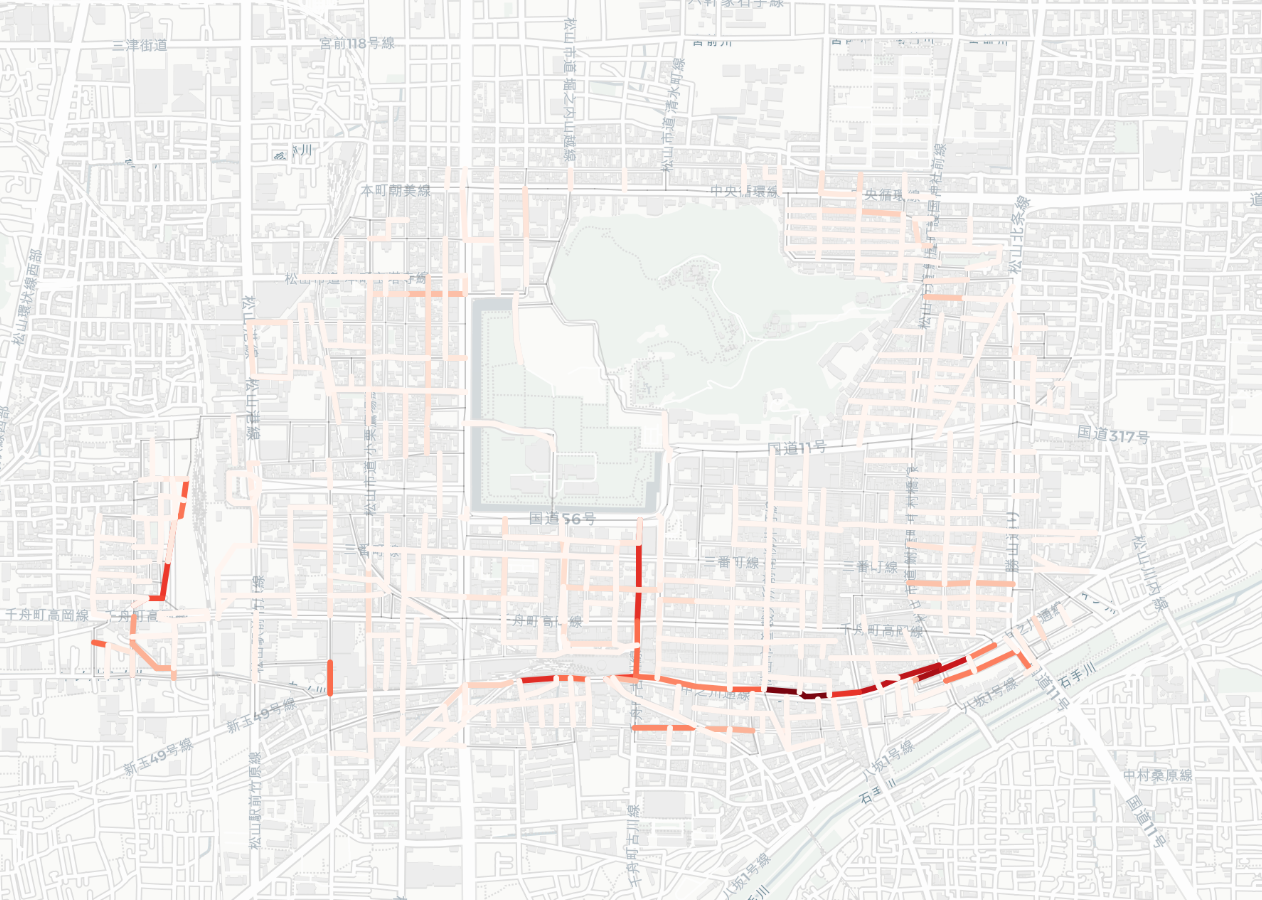
\includegraphics[width=\linewidth]{assets/assignment/pictureA.png}
  \captionof{計算結果を地図上に示したものです。図の色のついた道が消すことによって総旅行時間を減少させる道で、色が濃いほど減少効果が大きいことを示しています。}
  \label{fig:pictureA}
\end{center}


\subsubsection*{「中ノ川通り」閉鎖実験：なぜ主要幹線が渋滞を招くのか}

具体例として、松山市の主要幹線道路である「中ノ川通り」の東行き車線（松山市駅から離れる方向）に注目します。この道は片側3車線で交通量も多い区間ですが、シミュレーション上で図の青色の矢印付近のリンクを閉鎖したところ、全体の総旅行時間が約32分も短縮されるという結果が出ました。
交通の変化としては、中ノ川通りを閉鎖することで、それまで特定区間に集中していた交通が南北の隣接道路へと分散されます。
一見すると迂回によるロスが増えるように思えますが、閉鎖前、中ノ川通りの松山市駅付近（下図でむらさき色で囲った部分、閉鎖した区間よりも西側）において交通量が過剰であったために、この区間での時間ロスが大きくなっていました。
中ノ川通りの閉鎖によりこのむらさき色で囲った混雑区間の交通量が減少し、その減少効果は迂回による増加分を上回ったためにこのような結果が得られたと解釈しました。

\begin{center}
  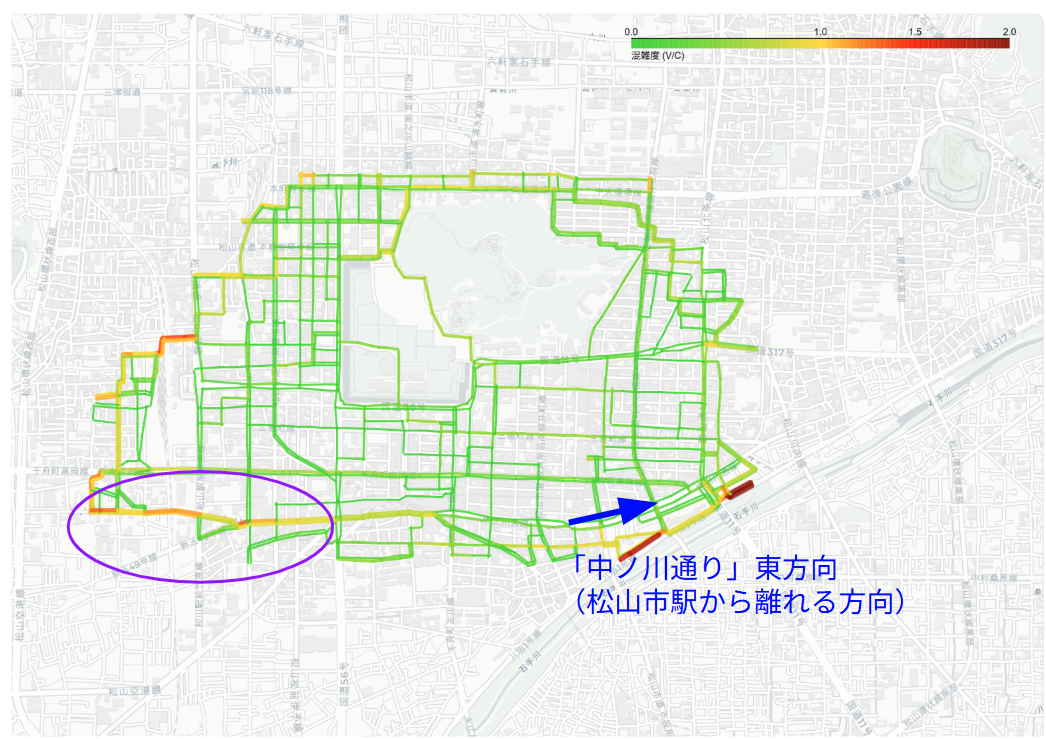
\includegraphics[width=\linewidth]{assets/assignment/pictureB.png}
  \captionof{各リンクの混雑度を図示したものです。オレンジ色や赤色のリンクが混雑していることを示しています。}
  \label{fig:pictureB}
\end{center}

\subsubsection*{JR松山駅高架化がもたらす効果}

現在進められているJR松山駅の高架化に合わせ、JR駅の下を通り抜ける道路が新設される計画となっています。
本検証では、実際に計画されているのと同じ駅を東西に貫く仮想道路（片側2車線、延長286m）を新設し、その影響を計測しました。その結果、都市全体の総旅行時間は18.89時間も減少するという結果が得られました。
新設道路により、既存の周辺道路の交通量は大きく変化します。シミュレーション上では、東行きで1249台、西行きで532台もの交通量が新設区間へと転換されました。
注目すべきは、これまで渋滞が激しかった特定区間の交通負荷を、新設リンクが「バイパス」として効率よく引き受けている（地図を拡大しているため分かりづらいですが、先ほどの図でむらさき色で囲ったリンクの交通量が大幅に減っている）点です。

\begin{center}
  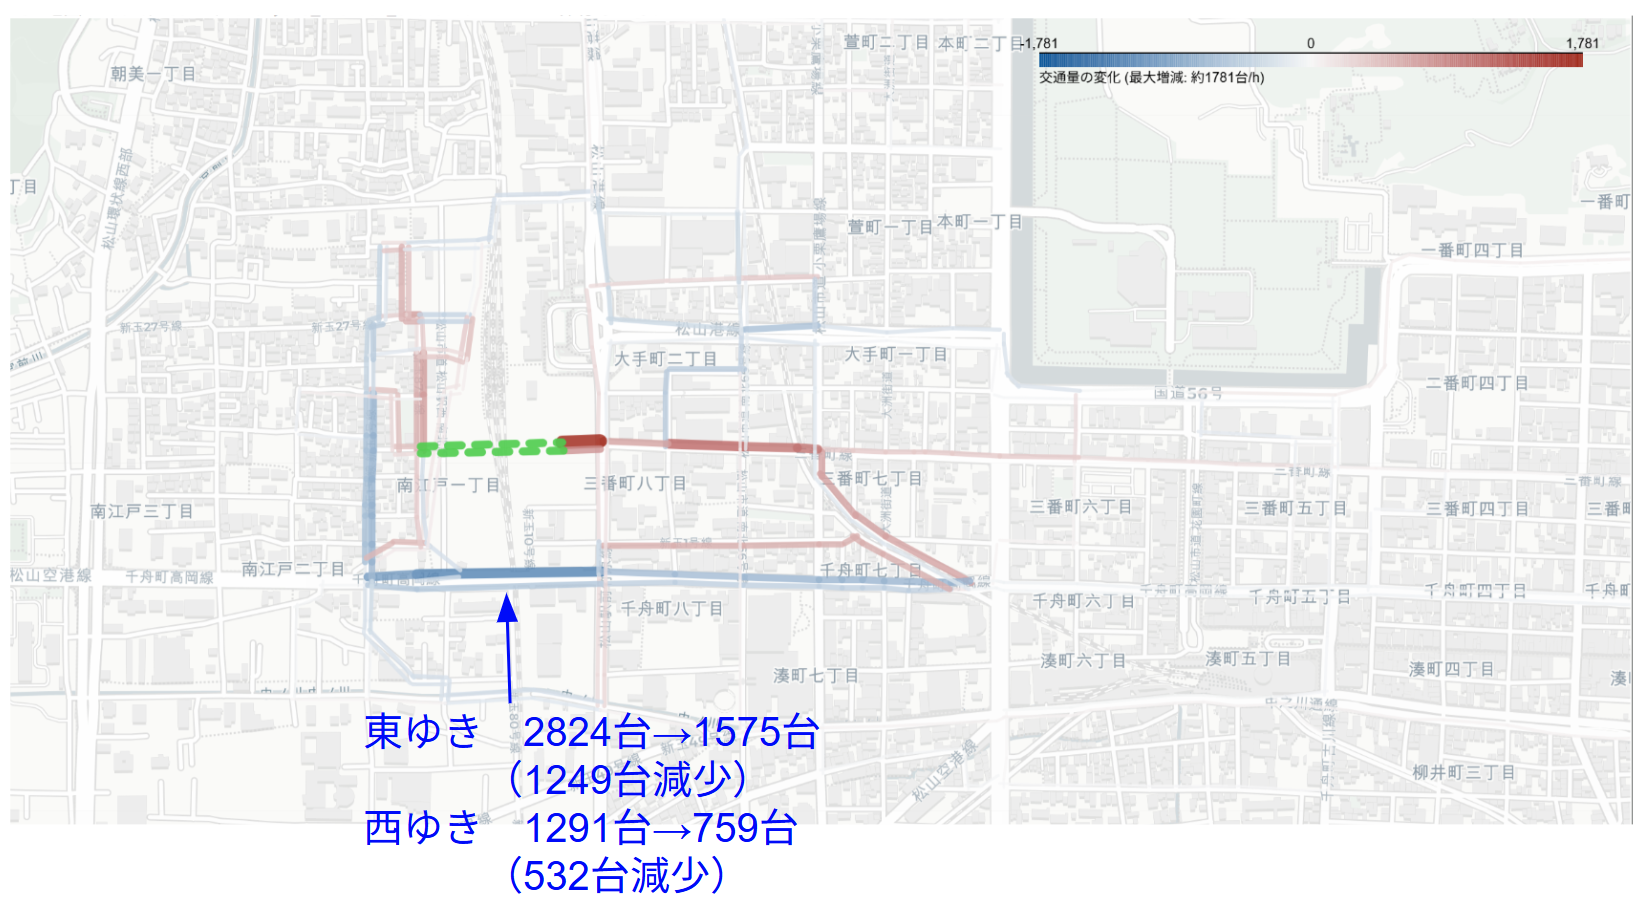
\includegraphics[width=\linewidth]{assets/assignment/pictureC.png}
  \captionof{黄緑色の点線が今回の検証で新設したリンク。この地図ではリンク新設の前後での交通量の増減を示しており、赤が増加・青が減少を示しています。}
  \label{fig:pictureC}
\end{center}

\subsubsection*{混雑緩和のメカニズム：下に凸の増加関数を攻略する}
なぜ、特定の地点への交通集中を緩和することが、これほどまでに大きな効果を生むのでしょうか。その鍵は、交通工学で用いられるリンクパフォーマンス関数（BPR関数）の性質にあります。
今回の計算に用いたリンクパフォーマンス関数は、本テキストでも既出の以下の式です。
\begin{equation}
  t_a(x_a) = t_{a0}\left\{1 + 0.15\left(\frac{x_a}{C_a}\right)^4\right\}
\end{equation}

これは交通量が増加するにつれ、旅行時間が急激に立ち上がる「下に凸の増加関数」です。つまり、渋滞ポイントで交通量を1台減らすことで得られる時間短縮効果が、空いている道路での1台の削減効果よりも圧倒的に大きくなります。
中ノ川通りの閉鎖による交通分散も、JR松山駅の新設道路によるバイパス効果も、本質的には「極端に混雑しているリンクの負荷を減らす」という点で共通しています。都市全体の旅行時間を最小化するためには、ボトルネックへの流入をいかに制御するかがポイントとなります。
　
\subsubsection*{結びに}
今回の検証は、松山市という実在の都市構造をモデル化することで、理論上のパラドックスが現実の都市計画においても十分起こり得ることを示唆しました。
道路を「消す」ことでも「加える」ことでも交通の流れを改善できる（逆に言えば悪化させる可能性もある）ということは、データに基づいたシミュレーションによる都市計画を進めることの重要さを示しています。

\end{column}
\clearpage



\input{chapters/assignment/ch6_dta.tex}

\input{chapters/assignment/ch7_evogame.tex}

\input{chapters/assignment/ch8_pigou.tex}

\input{chapters/assignment/ch9_simulation.tex}

\clearpage
\begin{column}{ミニ研究~東京都心部の道路網におけるsecond-best pricing~}

東京都心部（山手線の内側）の道路ネットワークを対象に，以下の分析を行った．

(1) Day-to-day ダイナミクスシミュレーションに基づき，
収束後の UE 状態における総旅行時間，リンクごとの旅行時間および交通量を算定した．

(2) 総旅行時間の短縮（SO 配分の目的関数）に基づいて
Pigouvian 課金を導出し，その課金を導入した状態で
Day-to-day ダイナミクスシミュレーションを行った場合，
総旅行時間が SO 配分と一致することを確認した．

(3) 課金可能リンクに限定して Pigouvian 課金を導入した場合について，
総旅行時間や社会的余剰の変化を分析した．

なお，使用したデータは山手線内側周辺の交通ネットワークデータ（幹線道路）と
2019年PT調査を基にしたOD交通量データである．
PT調査は標本調査であるため，
PTによって得られたOD需要は300倍している．
どの地域からの出発が多いか図示してみたところ，
文京区のあたりが最も多くなっていた．

\begin{center}
  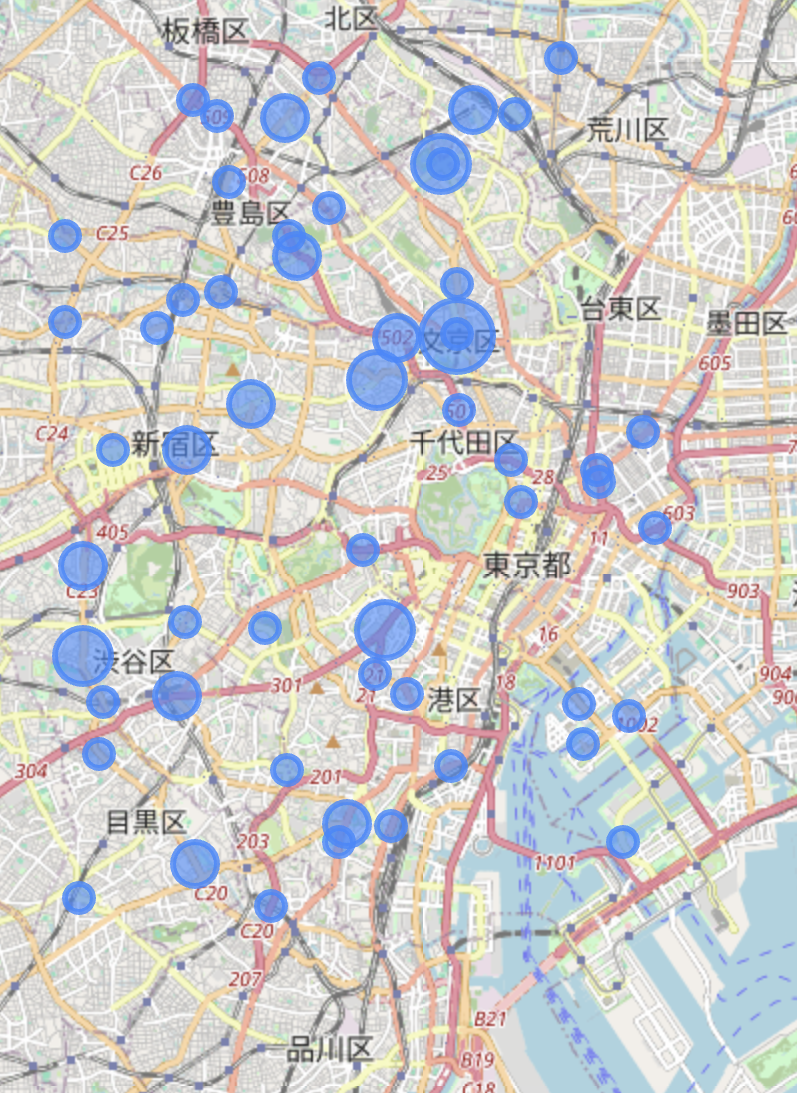
\includegraphics[width=0.5\linewidth]{assets/assignment/fig_column2/origin_distribution.png}
  \captionof{figure}{発地分布}
\end{center}

\vspace{4mm}

\textbf{(1) Day-to-day ダイナミクスによるUE状態の算定}

今回，day-to-dayダイナミクスは

\[
x^{t+1} = (1-\eta)x^t + \eta \cdot \mathrm{AON}(c(x^t)+\tau)
\]

という更新則に基づく．
これは，前日の経路コストを踏まえてAON配分が行われるが，
実際にその経路に動くのは一部
（今回であれば，10\%）であるということを示す．

AON配分は離散的な配分であり，
AON配分されるリンクが変化するたびに
総旅行時間は均衡点の付近でジグザグと変化する．

実際にこの更新則のもとで計算を回すと，
23100の総トリップは図のように収束し，
総旅行時間は2150.1078 [h$\cdot$台] となる．

\begin{center}
  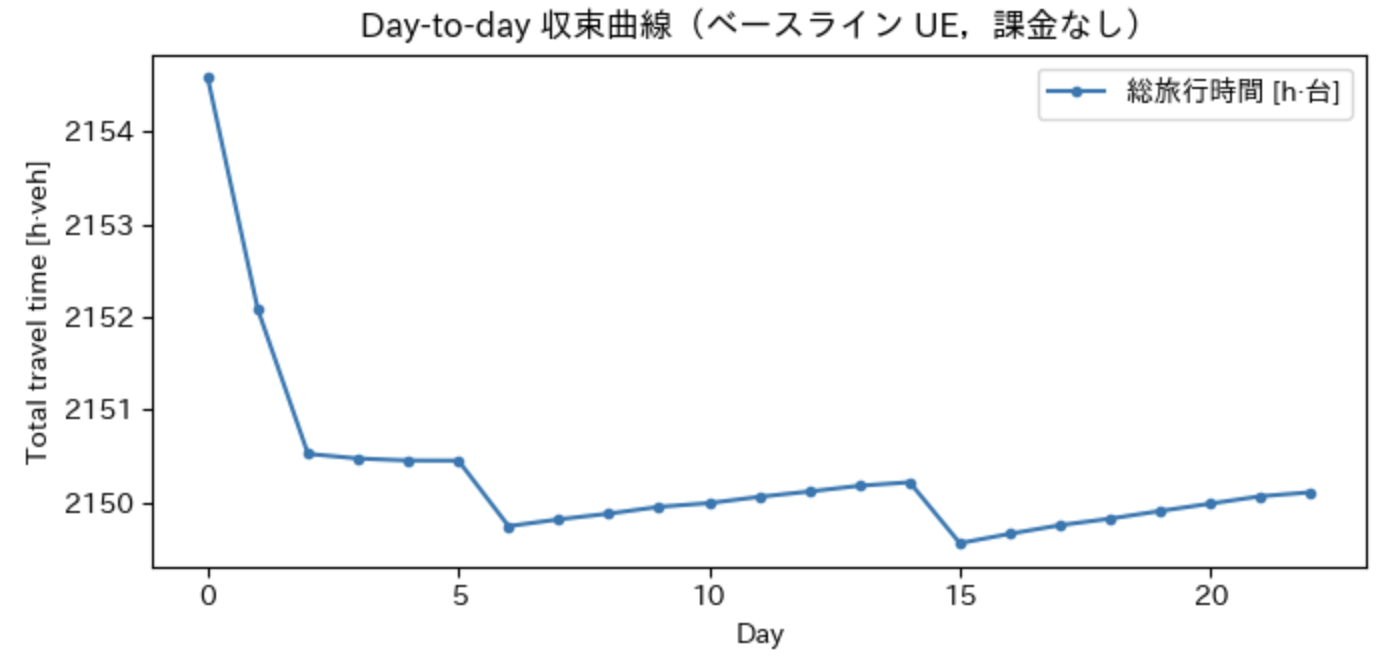
\includegraphics[width=\linewidth]{assets/assignment/fig_column2/day_to_day_ue.png}
  \captionof{figure}{Day-to-dayダイナミクスの収束}
\end{center}


また，均衡に達した際の道路の混み具合
（赤が混んでいる）を示すマップは以下のようになった．

\begin{center}
  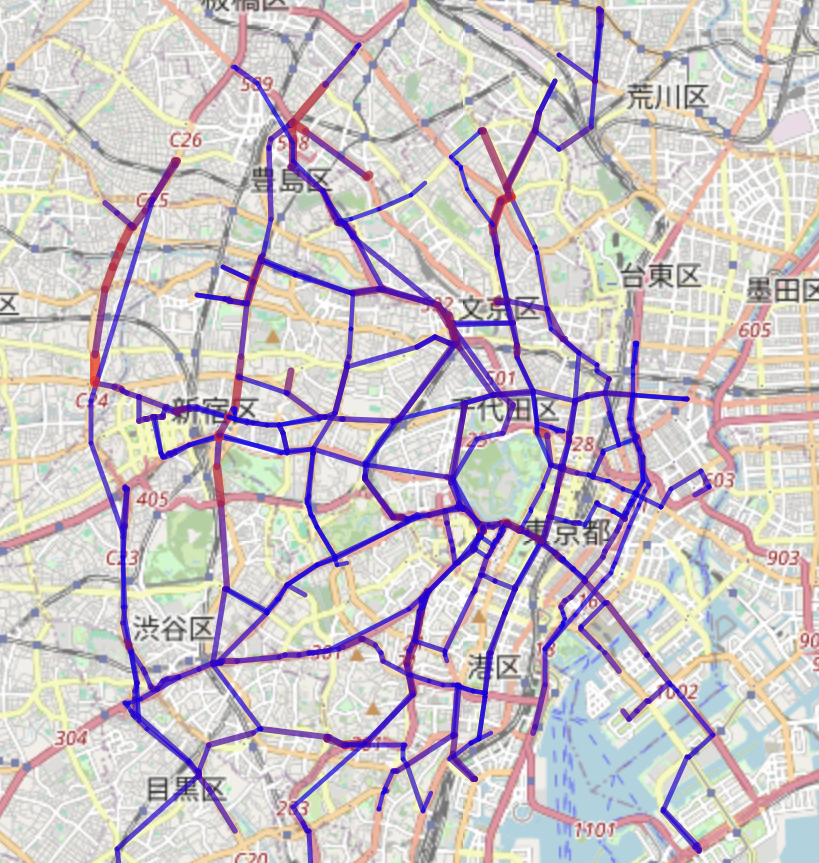
\includegraphics[width=0.5\linewidth]{assets/assignment/fig_column2/congestion_map.png}
  \captionof{figure}{UE状態におけるリンク混雑度}
\end{center}

さらに，最も混雑していた文京区向丘周辺を拡大すると，
以下のようになった．

\begin{center}
  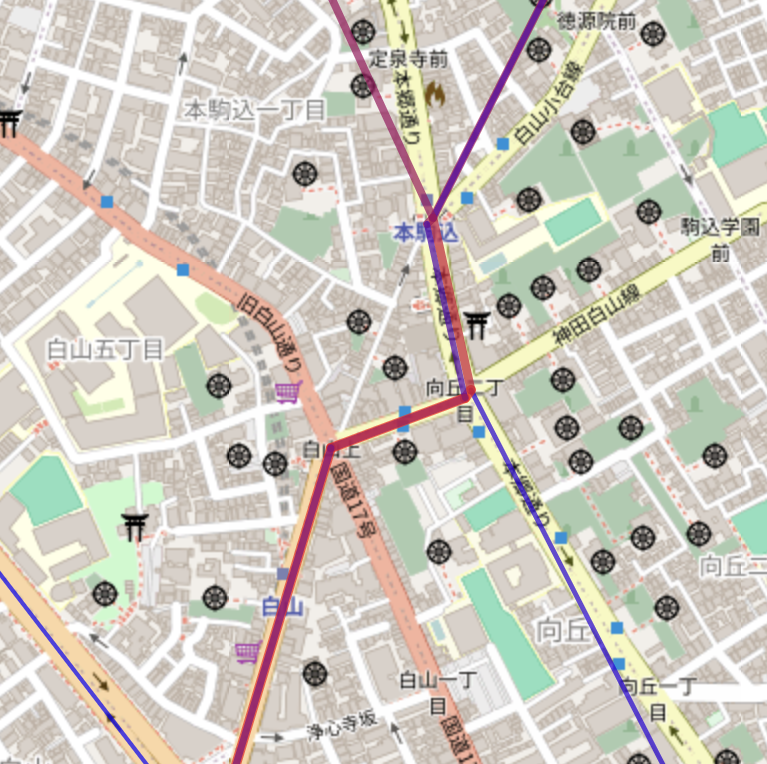
\includegraphics[width=0.5\linewidth]{assets/assignment/fig_column2/mukogaoka_map.png}
  \captionof{figure}{文京区向丘周辺の混雑状況}
\end{center}


混雑しているリンクはどちらかといえば北側に集中しており，
この過程のもとで最も混雑しているリンクは
文京区向丘周辺となった．

東京都心部の道路ネットワークは
千代田区を中心に放射状に広がっており，
それらをつなぐ環状線など，
複数の道路が入り込む場所の道路容量が少ない場合，
混雑する傾向にあり，
それが需要が多い北側であるとより顕著になる．

\vspace{4mm}

\textbf{(2) SO配分と課金状態でのDay-to-dayダイナミクス}

先ほどとは異なり，
総旅行時間の最小化を目的関数にとると，

\[
t_a(x_a) + t'_a(x_a)\cdot x_a
\]

をリンクコストとしてFrank-Wolfe法を用い
均衡を求めることができる．

総旅行時間は

\[
T_{\mathrm{SO}} = 2146.8598 \ [\mathrm{h}\cdot\mathrm{台}]
\]

となり，
その均衡を達成するために必要な課金額の最大値は
時間で表すと0.17分となる．

リンクごとに適切な課金を施し，
day-to-dayダイナミクスを回していくことで
SOと同じ配分結果を得ることができる．
これはほかでもなく，
課金によって外部性が内部化されている事を表す．

\begin{center}
  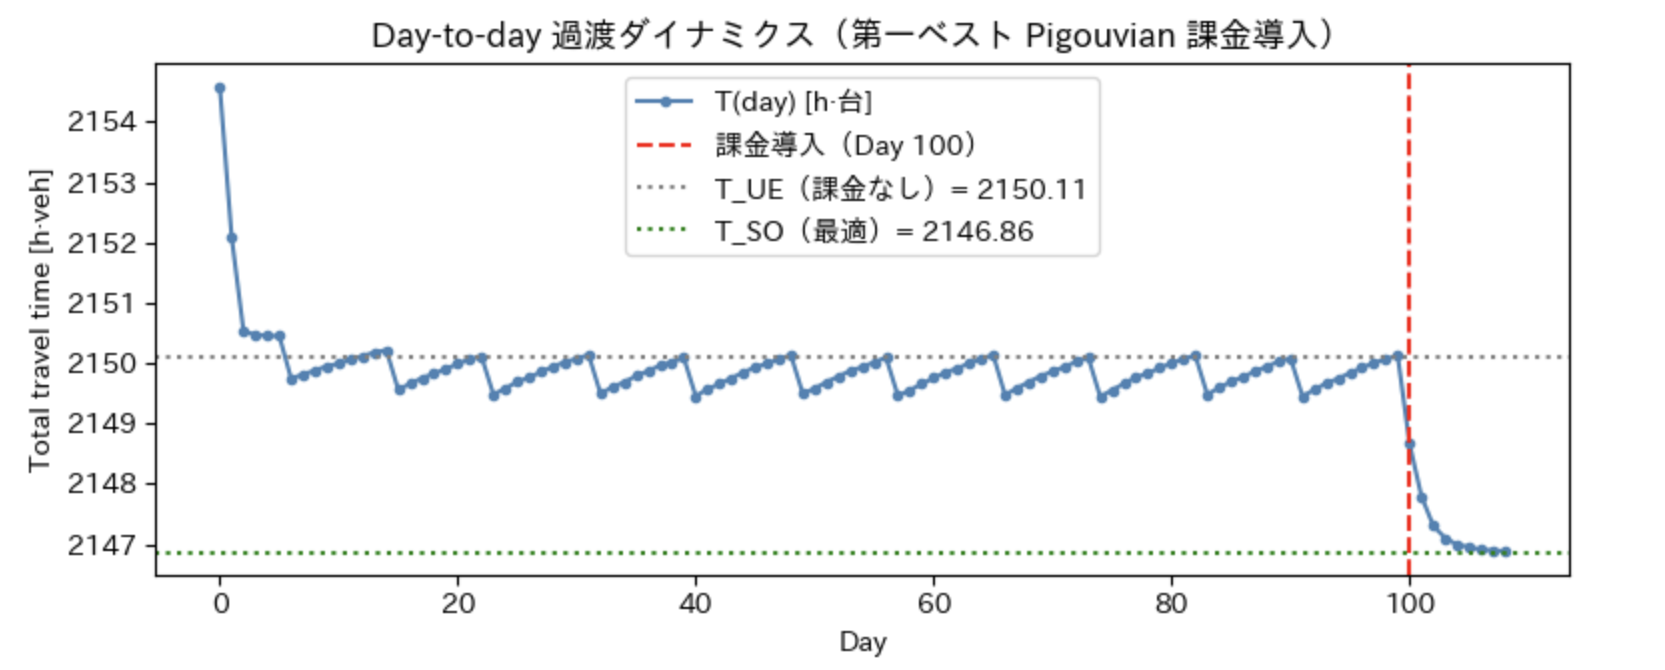
\includegraphics[width=\linewidth]{assets/assignment/fig_column2/day_to_day_first_best.png}
  \captionof{figure}{First-best課金下でのDay-to-dayダイナミクス}
\end{center}


この仮定のもとで最も課金されたリンクは
文京区本駒込ー動坂間のリンクであった．

文京区からの発地が多かったことや
この辺りのリンクのcapacityが小さいことなどから，
混雑し，かつ重要であるリンクに
より多くの課金がされることが確認できる．

\begin{center}
  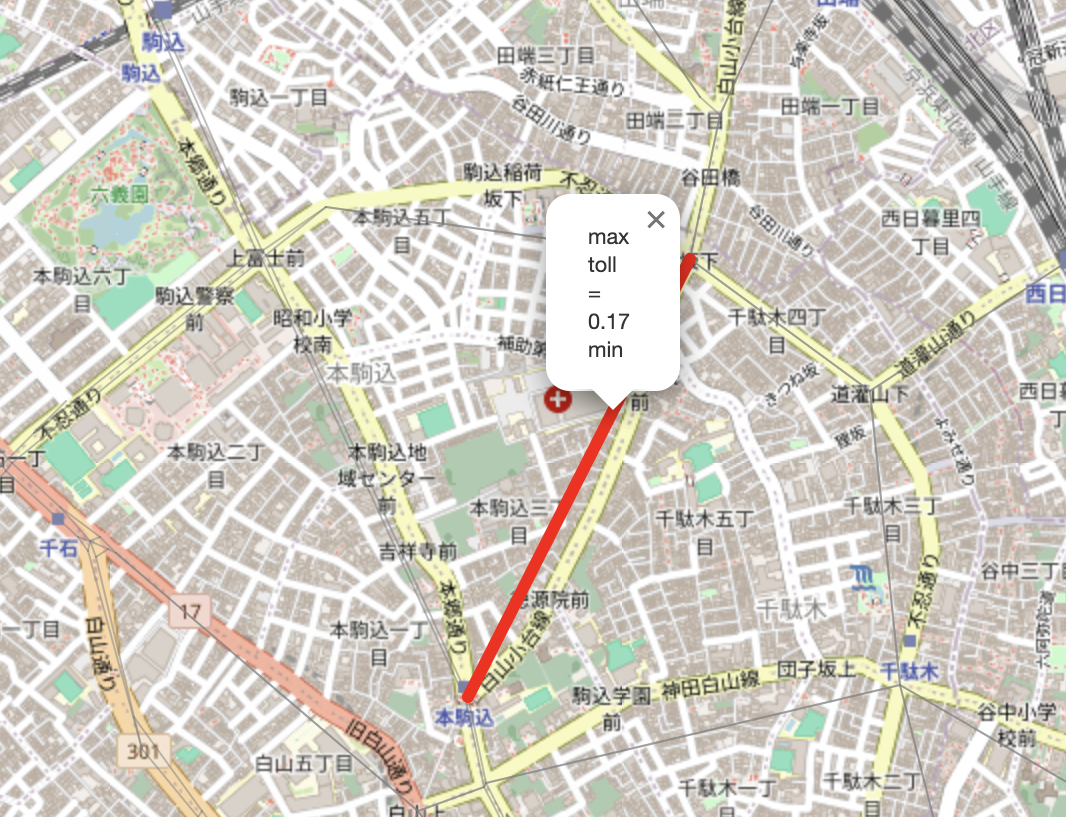
\includegraphics[width=0.5\linewidth]{assets/assignment/fig_column2/max_toll_link.png}
  \captionof{figure}{最大課金リンク周辺}
\end{center}


\vspace{4mm}

\textbf{(3) 課金可能リンクへの限定}

今回，
課金可能なエッジ数は全体のリンクの28\%であった
（国道などの幹線道路及び高速道路）．

それらのリンクに先ほど求めた
First-bestな課金を施すと，
総旅行時間は2150.0788 [h$\cdot$台] となり，
UEの時とほぼ変わらなくなってしまった．

先ほどのように
狭くて需要が集中しているリンクに
直接の課金ができないためであると考えられる．

\end{column}

\clearpage


\input{chapters/assignment/appendix.tex}

\addcontentsline{toc}{section}{参考文献}
\bibliographystyle{stone-ship}
\bibliography{../src/bibliography/assignment}

\chapter{行動モデル}
\chapterauthor{松永隆宏}

\chapter{はじめに}
\chapterauthor{羽藤英二}

人口減少が進んでいた地方都市を襲った巨大災害直後の破壊の風景の中に立ったとき，何かできたことはなかったか，どうすればよかったのかと思わずにはいられなかった．今，都市と交通を学ぶことにどのような意味があるのだろうか．あるいは激変する社会の中で今私たちに何ができるだろうか．おそらくそれは，道路や鉄道，駅前広場や沿道空間の形を単に学ぶことではない．現実の空間とネットワークの上で，人びとがLLMが得意とする言語のやりとりを超えて「空間」をどのように認知し，選択し，互いに影響し合い，その集積として流れ$=$交通が生まれ，外部不経済としての混雑や滞留，さらには回遊，分断，格差がどのように発生しているのかを捉え直すことである．そして，よりよい理解に基づく行為の反復の果てに，都市空間そのものの価値と構造が歴史的な過程を通じていかにその地理的関係が変容していくのか，徹底的に理解することなくして，いかなる政策も計画も設計もサービスも，威勢のいい掛け声をかけたところで何も変わらないのではないだろうか．

行動モデル，ネットワーク配分，最適化，機械学習という本書の四つの柱は，この過程を，個人の意思決定から社会的な空間変容まで貫いて理解するための基礎理論である．本書の目的は，それらを別々の計算技術として紹介することではない．研究の作業と思考の往復のなかで私たちが考えてきたように，人びとの選択の連鎖がネットワーク現象を生成し，その現象を変えようとしてなされる現実の都市設計や交通計画の行為が，再び人びとの行動そのものを変え，その反復が都市自体を更新していく．この連関を，私たち自身が経験してきた都市設計，交通計画，そしてそれらを下支えする基礎理論の構築と実証の蓄積を踏まえながら，ひとつの連続した知の体系として描き直すことに本書の狙いがある．

その出発点のひとつが，\citet{McFadden1974}によって基礎づけられた離散選択理論である．2000年のノーベル経済学賞へと結実したこの理論は，人はなぜこの経路を選び，この交通手段を選び，この場所へ向かうのかという問いに対し，効用と確率的選択という考え方によって，個人の意思決定を政策や空間設計に応答する構造として厳密に記述する道を開いた．こうして離散選択モデルは世界中の交通計画に利用され，インフラ整備の基礎理論として定着するに至った．ここで重要なのは，ネットワーク上の行動が単なる心理学的記述にとどまらず，制度変更や空間条件の変化に対して地理的分布として応答する対象となったことである．この視点があったからこそ，交通行動は社会基盤計画の中心に置かれ，公共交通計画，都市計画，駅まち設計，自動車交通制御に共通する理論的基礎が築かれたといえよう．

しかし，個人の選択を理解するだけでは都市は見えない．選択はネットワーク上で重なり合い，混雑，所要時間，遅延，容量制約，乗換え負荷，滞在時間といった現象へと変換されるからである．マルコフ過程はこうした行動の連鎖を記述する上で最も基礎的な理論であり，最短経路探索，利用者均衡，確率的配分，動的配分と結びつくことでネットワーク上の行動記述という点で大きな力を発揮することとなった．\citet{Wardrop1952}と\citet{Beckmann1956}は，この問題をネットワーク上の均衡として定式化する道を拓いた．さらに，物流や配車，公共交通運用に目を向ければ，単なる経路選択にとどまらず，誰がどの需要をいつどの順序で担うかという組合せ設計が前景化し，\citet{DantzigRamser1959}以来の VRP，さらには列生成，双対問題，\citet{Benders1962}に代表される分解法が，現実の大規模問題に対抗するための基礎となってきた．こうしたアルゴリズムの実装は，線形代数に基礎づけられた行列計算によって支えられている．そして近年では，ChatGPT の登場によって，その実装や試行錯誤が以前よりはるかに身近なものとなったといってよいだろう．

さらに，現実の交通と都市は，唯一の均衡点に収束する静的な系としてではなく，学習し適応する動的な系として再定義されるべきであろう．制度が変われば人は行動を変え，情報が変われば期待も変わる．\citet{Sandholm2002,Sandholm2010}による人口ゲームと進化動学は，この適応の反復そのものを理論化した点で，従来の均衡配分を決定的に拡張する契機となった．さらにいえば，交通政策とは，ある時点の均衡をずらす一度きりの操作ではない．人びとの模倣，学習，反応，慣性の上に新たな安定状態を形成していく過程への介入なのである．近年の Matsunaga and Hato（2026）は，この系譜を受け継ぎつつ，部分可制御性の下で平均場的インセンティブと逆オークションを結びつけ，都市鉄道混雑制御を設計問題として捉え直している．そこでは，限られた予算，私的情報，日々の適応，平均場的結合が，ひとつの閉ループ系として統合されつつある．

同時に，日々の経路変更や需要変動を実証的に捉えるには，個票レベルの長期観測と，それを扱いうる学習理論が必要になる．Ogawa and Hato（2026）は，1か月規模の個人 GPS 軌跡から日々の経路変更を捉え，Temporal Boltzmann Machine と Graph Attention Network，さらに correlated equilibrium の制約を組み合わせることで，共有情報に対する異質で相関した適応反応を表現しようとしている．ここで重要なのは，深層学習を単なる高精度予測器として用いるのではなく，信念更新や相関した適応の代理構造をもつ実証モデルとして位置づけている点である．学習は理論を置き換えるのではなく，理論が十分に捉えきれてこなかった観測の厚みに踏み込むための手段となる．

この文脈の上に，Transformer や大規模言語モデルを起点とする近年の AI の急速な発展が重なる．\citet{Vaswani2017}以降，系列の長距離依存を捉える注意機構，表現学習，生成モデルは，活動スケジュール，経路系列，都市記述，需要変動の理解に新しい可能性を開いた．さらに，物理法則や保存則を学習に埋め込む PINN は，\citet{Raissi2019}以降，データ駆動型学習と数理モデルの橋渡しとして注目されている．しかし，ここで立ち止まらなければならない．都市と交通の本質は，言語の中だけに存在するのではない．人は文を読んで移動するのではなく，身体をもち，制約を受け，他者と干渉し，空間の抵抗や誘因の中で行動する．そして，その行動は実際にネットワーク負荷を変え，土地利用を変え，拠点の価値を変え，都市そのものを作り替えてしまう．私たちは世界各地の現実の都市や駅を設計し，交通計画を評価し，都市計画に取り組んできた．

その経験から考えるとき，既存の理論はなお，本質的な都市の問題を記述するには十分ではないのではないか．たしかに LLM は強力である．しかしなお最終理論としての弱点がないわけではない．都市と交通に必要なのは，LLM の基盤となる「言語」を超えて，現実の「空間」に作用する物理的な選択，相互作用，制約，学習，設計を統合する理論である．人の行動がネットワーク上でどのように干渉し合い，その反復がどのように都市の形を変え，さらにその変わった都市が次の行動をどのように規定するのか．この循環を捉えるには，効用理論，均衡理論，進化動学，最適化，深層学習，さらには物理制約までを横断しなければならない．都市を「語れる」知能ではなく，都市を「説明し，予測し，設計できる」知能をめぐって世界中の研究者たちが訥々と自分たちの課題と向き合い続けている．

最前線のひとつは自動走行であろう．従来のルールベースを超える E2E 的発想では，周囲の行動を外生的に予測し，その上で自車だけを最適化すればよいと考えられがちであった．しかし実際の交通は，相手もまたこちらを見て応答する相互作用の場である．Furuhashi and Hato（2026）は，この限界を正面から捉え，予測依存型の制御から，相互作用そのものを均衡埋め込みで扱う I2I 型の自動運転へと理論の重心を移している．そこでは，shared constraints の下での variational generalized Nash equilibrium，ICNN による学習可能なコスト設計，そして equilibrium-embedded predictive control が統合され，E2E を越えて現実空間の内生性に向き合う知能の姿が模索されている．さらに彼らは，この枠組みを，これまでにない歩行者と自動走行の混在空間における最適制御と最適設計の理論へと拡張しようとしている．

本書が学部生・大学院生に伝えたいのは，まさにこうしたダイナミックな研究のプロセスとその基礎となる理論のバリエーションである．行動モデル，ネットワーク配分，最適化，機械学習は，互いに隣接する技法ではない．それらは，人間の行動がネットワークを通じて都市を変え，その都市の設計が再び人間の行動を変えるという現実の循環構造に迫ろうとする，ひとつの知の系譜である．\citet{McFadden1974}から\citet{Wardrop1952}，\citet{Beckmann1956}，\citet{Sandholm2010}，\citet{Vaswani2017}，\citet{Raissi2019}へと至る流れは，単なる理論の並列ではなく，観測，均衡，設計，学習を再接続し続けてきた歴史である．そして Matsunaga and Hato（2026），Ogawa and Hato（2026），Furuhashi and Hato（2026）に見られるように，その流れは今，公共交通計画，日々の経路選択，自動走行の制御という異なる対象を通じて，新たな段階に入りつつある．理論を下敷きに新たな駅まち空間を設計しなおすこと．格差を是正しうる公共交通を構想し導入すること．今までにない都市と地域を構想し，計画し，実装し，運営すること．そのための基礎理論を，本書を通じて学んでもらいたい．都市と交通を学ぶとは，変わりゆく現実を理解するだけでなく，失われつつある場所と壊れた風景の前で，それでもなお次の危機に向けた新たな空間を構想し直す力を身につけることなのである．


\addcontentsline{toc}{section}{参考文献}
\bibliographystyle{stone-ship}
\bibliography{../src/bibliography/intro}

\input{chapters/behavior_modeling/ch1-rut}
\input{chapters/behavior_modeling/ch2-correlation}
\clearpage
\begin{column}{ミニ研究のすすめ}{石河万衣}
    
　行動モデルは政策議論等の基盤となるが、本稿ではその構築過程における試行錯誤に着目する。
具体的には、松山市のPT調査データを用い、以下の効用関数を設定して交通手段選択モデル（自動車、鉄道、バス）を推定した。
\begin{align*}
U_{train} &= \beta_{time} x_{time} / 10 + \beta_{fare} x_{fare} / 100 + \beta_{train}\\
U_{bus} &= \beta_{time} x_{time} / 10 + \beta_{fare} x_{fare} / 100 + \beta_{bus}\\
U_{car} &= \beta_{time} x_{time} / 10 + \beta_{fare} x_{fare} / 100
\end{align*}

　以下の結果から、初期のMNLモデルでは運賃パラメータが正となり、運賃上昇が効用を増加させるという実態に反する結果を示した。

　そこで運賃に対数変換を施し再推定したところ、尤度が改善し全パラメータの符号が整合した。
これにより、低価格帯では運賃変動の影響が大きく、高価格帯では相対的に小さいという非線形の性質を適切に捉えることができた。

　さらに、まず「自動車」か「公共交通」を選び、後者の場合に「鉄道」か「バス」を選ぶ階層的プロセスを想定し、NLモデルを推定した。
MNLモデルより尤度がさらに向上し、スケールパラメータ$\lambda$も有意となった。これにより誤差項間の無相関仮説が棄却され、
本対象におけるネスト構造導入の妥当性が統計的に実証された。

\begin{center}
    \captionof{table}{交通手段選択モデル（$N$=1,902）}
    \label{tab:integrated_model}
      
    \small
    \setlength{\tabcolsep}{3pt}

    \begin{tabular}{l c r@{\,}l c r@{\,}l c r@{\,}l}
    \toprule
       & \multicolumn{3}{c}{MNL} & \multicolumn{3}{c}{MNL（運賃対数）} & \multicolumn{3}{c}{NL（運賃対数）} \\
       & パラメータ & \multicolumn{2}{c}{t値} & パラメータ & \multicolumn{2}{c}{t値} & パラメータ & \multicolumn{2}{c}{t値} \\
    \midrule
    $\beta_{train}$ & 0.161 & 0.958 & & 0.809 & 2.882 & ** & 0.478 & 1.710 & \\
    $\beta_{bus}$   & -0.980 & -5.609 & *** & -0.310 & -1.059 & & -0.258 & -1.130 & \\
    $\beta_{time}$  & -0.431 & -7.546 & *** & -0.393 & -7.509 & *** & -0.361 & -7.543 & *** \\
    $\beta_{fare}$  & 0.071 & 1.530 & & -0.672 & -2.764 & ** & -0.364 & -1.657 & \\
    $\lambda$       & - & \multicolumn{2}{c}{-} & - & \multicolumn{2}{c}{-} & 0.551 & 4.687 & *** \\
    \midrule
    初期対数尤度 $L(0)$ & \multicolumn{3}{c}{-1599.214} & \multicolumn{3}{c}{-1599.214} & \multicolumn{3}{c}{-1599.214} \\
    最終対数尤度 $L(\beta)$ & \multicolumn{3}{c}{-1080.426} & \multicolumn{3}{c}{-1077.551} & \multicolumn{3}{c}{-1072.256} \\
    決定係数 $\rho^2$ & \multicolumn{3}{c}{0.324} & \multicolumn{3}{c}{0.326} & \multicolumn{3}{c}{0.330} \\
    修正済み決定係数 $\bar{\rho}^2$ & \multicolumn{3}{c}{0.322} & \multicolumn{3}{c}{0.324} & \multicolumn{3}{c}{0.326} \\
    \bottomrule
    \multicolumn{10}{l}{\footnotesize ***: $p < 0.001$, **: $p < 0.01$, *: $p < 0.05$} \\
    \end{tabular}
\end{center}

\end{column}
\clearpage
\input{chapters/behavior_modeling/ch3-choiceset}
\clearpage
\begin{column}{コラム}



発表時間内で紹介しきれなかったログサム分布の導出について記載する．
最大値の分布もまたガンベル分布で記述できるため，閉じた形で計算できることが大きなメリットである．


\section{ログサム分布の導出}

\subsection{最大効用の分布関数}

各選択肢 $j$ に対して効用を
\[
U_j = v_j + \tilde{\varepsilon}_j
\]
とし、最大効用を
\[
M = \max_j U_j
\]
とする。

任意の $x$ に対して、
\[
\Pr(M \le x)
=
\Pr(v_j + \tilde{\varepsilon}_j \le x, \ \forall j)
\]

誤差項が独立であることから、
\[
\Pr(M \le x)
=
\prod_j \Pr(\tilde{\varepsilon}_j \le x - v_j)
=
\prod_j F_j(x - v_j)
\]

ここで $\tilde{\varepsilon}_j$ が Gumbel 分布に従うとすると、その累積分布関数は
\[
F_j(z)
=
\exp\left[
-\exp\{-\alpha(z - \beta)\}
\right]
\]
である。

したがって、
\[
\Pr(M \le x)
=
\prod_j
\exp\left[
-\exp\{-\alpha(x - v_j - \beta)\}
\right]
\]

\[
=
\exp\left[
-\sum_j \exp\{-\alpha x + \alpha v_j + \alpha \beta\}
\right]
\]

ここで
\[
\omega(V) := \sum_j e^{\alpha v_j}
\]
とおくと、
\[
\Pr(M \le x)
=
\exp\left[
-\exp\{-\alpha x + \alpha \beta + \ln \omega(V)\}
\right]
\]


\subsection{位置母数へのログサムの出現}

上式は次のように書き直せる：
\[
\Pr(M \le x)
=
\exp\left[
-\exp\left\{
-\alpha \left(
x - \beta - \frac{1}{\alpha} \ln \omega(V)
\right)
\right\}
\right]
\]

したがって、$M$ は再び Gumbel 分布に従い、その位置母数は
\[
\beta^\ast
=
\beta + \frac{1}{\alpha} \ln \omega(V)
=
\beta + \frac{1}{\alpha} \ln \sum_j e^{\alpha v_j}
\]
となる。

すなわち、ログサムは最大効用の分布における位置母数として現れる。

\subsection{期待値としてのログサム}

Gumbel 分布
\[
\exp\left[
-\exp\{-\alpha(x - \beta^\ast)\}
\right]
\]
の期待値は
\[
E[M] = \beta^\ast + \frac{\gamma}{\alpha}
\]
である。ただし $\gamma$ はオイラー定数である。

よって、
\[
E\left[\max_j (v_j + \tilde{\varepsilon}_j)\right]
=
\beta + \frac{\gamma}{\alpha}
+
\frac{1}{\alpha} \ln \sum_j e^{\alpha v_j}
\]
を得る。

\end{column}
\clearpage

\input{chapters/behavior_modeling/ch4-abms}
\clearpage
\begin{column}{コロナ前後における活動の変化}
\subsubsection{MDCEVモデルとRecursive Logit Modelの比較}
（構造型モデルである\textbf{MDCEVモデル}と\textbf{Recursive Logit Model}の比較を行った.
\textbf{MDCEVモデル}は，1日を観測単位として，活動への時間配分を「離散的な活動洗濯＋連続的な時間配分」として定式化するものである．
一方で，離散選択モデルである\textbf{Recurisive Logit Model}は1日を時間ステップ列とみなし，1ステップ列からの遷移列から学習するものである．場所次元と過去活動の効果は両方とも無視するものとし，「時間配分」と「時系列推移」の2つのモデルでそれぞれ何を表現するか，できるかを比較する
東京都市圏で実施された4つのPPデータを使用するものとする．
\begin{table}[htb]
\centering
\caption{東京都圏で実施された4つのPP調査}
\label{tab:pp-survey-tokyo}
\begin{tabular}{c l l r}
\hline
period & \multicolumn{1}{c}{期間} & \multicolumn{1}{c}{文脈} & \multicolumn{1}{c}{n\_users (raw)} \\
\hline
1 & 2019-07-08 .. 2020-02-11 & \textbf{コロナ前} & 305 \\
2 & 2021-10-03 .. 2021-11-25 & \textbf{コロナ規制明け直後} & 115 \\
3 & 2022-12-19 .. 2023-01-30 & コロナ後・冬 & 182 \\
4 & 2023-11-15 .. 2023-11-29 & コロナ後・秋 & 223 \\
\hline
\end{tabular}
\end{table}

活動カテゴリとしては，H(home)，S(Shopping)，W(Commute/Work)，W2(Business)，O (Other)，予算制約はT=24hとする．
\begin{center}
  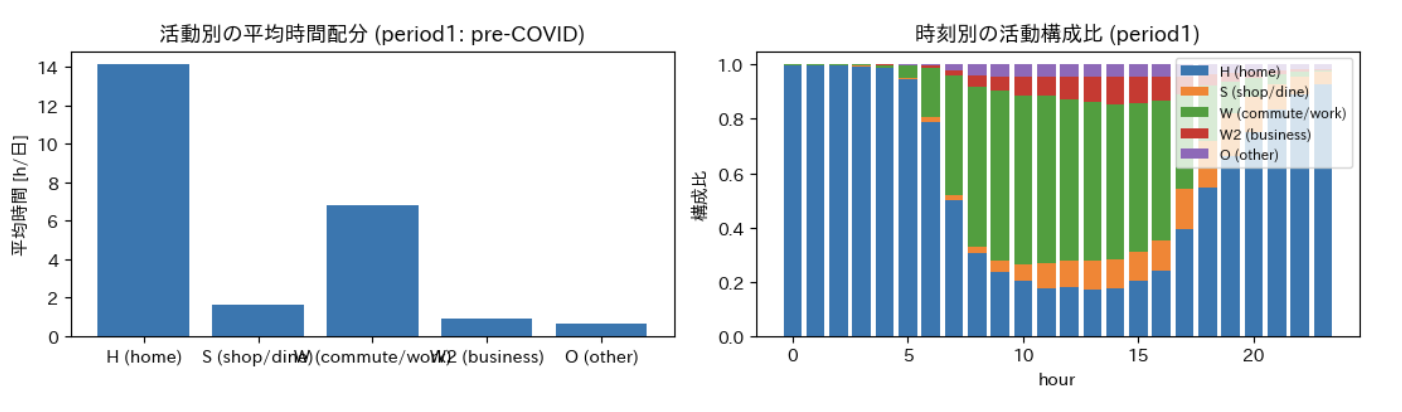
\includegraphics[width=\linewidth]{assets/behavior_modeling/column3/ABMS01.png}
  \captionof{figure}{実データの活動別グラフ}
  \label{fig:label-of-this-figure}
\end{center}

\subsubsection{MDCEVモデル（γ-profile, Bhat 2008)}

各out活動について，
\begin{equation}
V_k = \psi_k - \log(x_k / \gamma_k + 1)
\end{equation}
ここで，
\psi_k：ベース効用
\x_k:費やした時間
\gamma_k：飽和パラメータ
である．

選択確率は，以下の閉形式で表される．
\begin{equation}
P(x) = \left[ \prod_{k \in M} \frac{1}{x_k + \gamma_k} \right] \cdot \left[ \sum_{k \in M} (x_k + \gamma_k) \right] \cdot \left[ \prod_{k \in M} \frac{e^{V_k}}{\sum_j e^{V_j}} \right]
\end{equation}

\subsubsection{Recursive Logit Model}
時間tにおける活動，遷移効用を「1時間ごとに次の行動を決める」形で捉えるものとする．
\begin{equation}
U_t(i \to j) = \alpha_j + \delta_{\text{stay}} 1[j = i] + \delta_{\text{morn}} 1[i = H, j \neq H, 6 \leq t < 10] + \delta_{\text{eve}} 1[i \neq H, j = H, 17 \leq t < 22]
\end{equation}

\subsubsection{分析結果}
\textbf{MDCEVモデル}
\begin{center}
  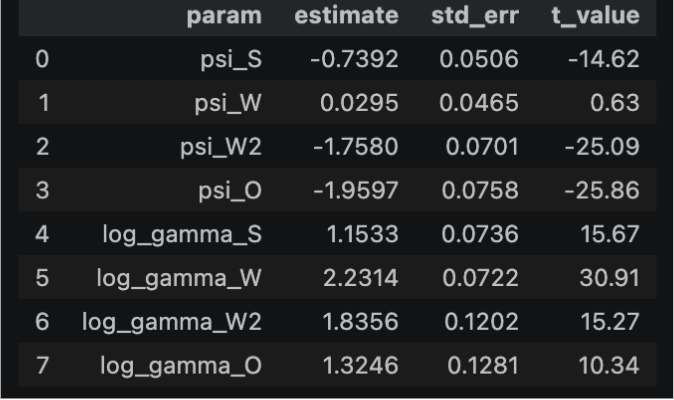
\includegraphics[width=\linewidth]{assets/behavior_modeling/column3/ABMS02.png}
  \captionof{figure}{MDCEVモデル preコロナ_MDCEVモデル推定表}
  \label{fig:label-of-this-figure}
\end{center}

ベース効用：Hは基準で0であり，ほとんどの活動で0以下なので何もしなければ選ばれにくいことがわかる．
飽和パラメータ：全てプラスの値であり，値が大きいほど，長く続く行動であることがわかる．
t値：絶対値が1.96を越えていればそのパラメータは5％優位水準で有意である．
仕事のベース効用（唯一正の値）が大きいので、仕事に行く動機は他の活動と比べて強い．飽和パラメータが大きいので、仕事は一度始めると比較的長く続くが、買い物、その他は比較的短く切り上げる
仕事のt値は低いが、自宅との値の差が小さいためと考えられる．

\textbf{Recursive Logit Model}
\begin{center}
  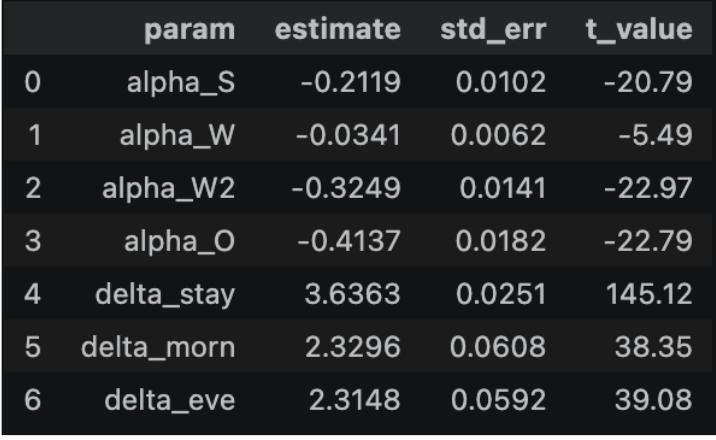
\includegraphics[width=\linewidth]{assets/behavior_modeling/column3/ABMS03.png}
  \captionof{figure}{RecursiveLogitModel_推定表}
  \label{fig:label-of-this-figure}
\end{center}
ベース効用：Hが基準で0以下なので何もしなければ選ばれにくい
活動継続のボーナス：同じ活動の続けることへのボーナス
朝の外出ダッシュ：6~10時の間に自宅を出るボーナス
夕方の帰宅ダッシュ：17~22時の間に自宅に帰るボーナス

delta-stayのt値が突出して高く，一度始めたら進行し続けることが言える．朝の外出と夕方の帰宅に強いバイアスがあることがわかる．

\textbf{再現性}
モデルから観測時間配分の再現を試みると，RL：推定パラメータのもとで各user,dayをt＝0からforward simuateする．
ほとんど完全に表現できていると言える．朝の外出項などが時間制約の学習に役立っていることがわかる．
\begin{center}
  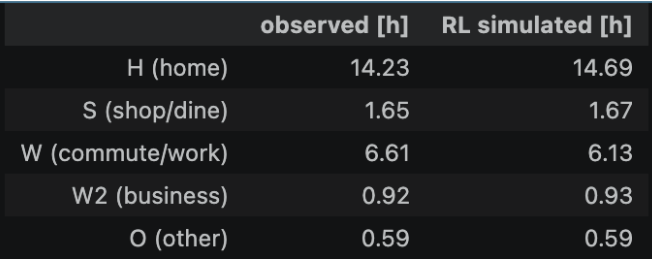
\includegraphics[width=\linewidth]{assets/behavior_modeling/column3/ABMS04_RL.png}
  \captionof{figure}{RLモデル推定表}
  \label{fig:label-of-this-figure}
\end{center}

\begin{center}
  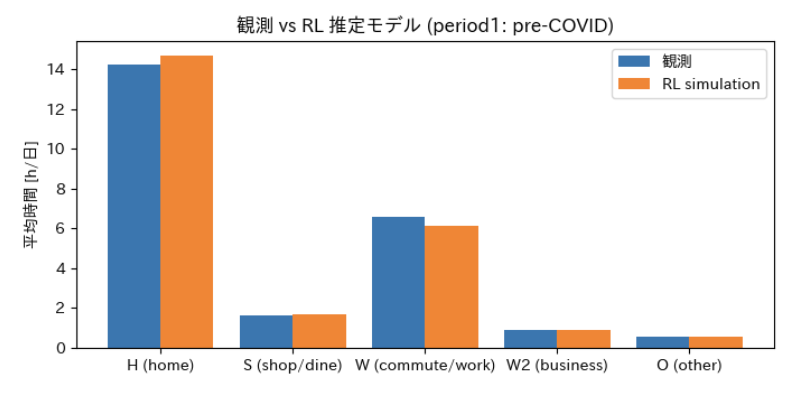
\includegraphics[width=\linewidth]{assets/behavior_modeling/column3/ABMS05-RL.png}
  \captionof{figure}{観測とRLモデルの比較}
  \label{fig:label-of-this-figure}
\end{center}

\textbf{MDCEVとRLの比較}
両方のモデルから観測時間配分の再現を試す．MDCEVモデルで推定された\gamma_kから求まる期待時間と，
観測モデルが異なるため，直接比較することはできないが，パラメータの符号と各活動の相対的な魅力度の傾向（\gamma_k，\alpha_kは一致する．
\begin{center}
  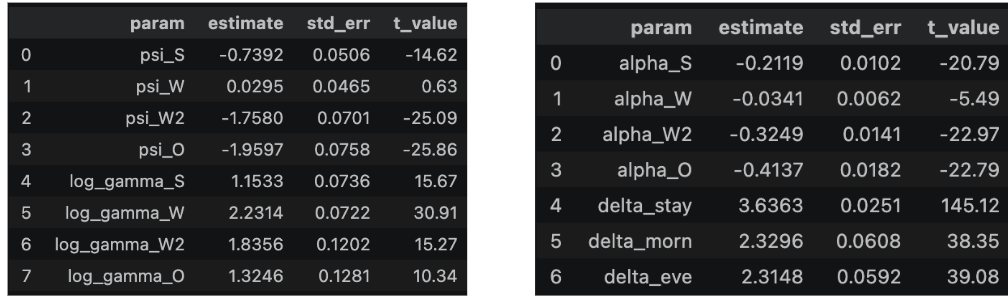
\includegraphics[width=\linewidth]{assets/behavior_modeling/column3/ABMS06.png}
  \captionof{figure}{MDCEVとRL推定表の比較}
  \label{fig:label-of-this-figure}
\end{center}

\subsubsection{時期による比較}
\textbf{実データを用いた比較}
・家にいる時間はコロナ規制後（直後ではなく少し経ってから）1時間程度長くなっており仕事、通勤時間は減少した．
コロナ規制後から普及した各種オンラインサービスの普及により、対面での仕事が減少したのだろうと考えられる．
・Business（業務）は、コロナ規制直後〜翌年の冬にかけて半減していることがわかるが、翌年の秋には元の水準に復活している．
・買い物に使う時間30分程度増加した．通勤時間が減り，通勤のついでで買い物に行く，ということが減って必要な時間が増えた．
\begin{table}[htb]
\centering
\caption{各Phaseにおける観測活動時間}
\label{tab:observed-activity-time}

\begin{tabular}{lcccc}
\hline

&
\begin{tabular}[c]{@{}c@{}}Phase1\\ コロナ前\end{tabular}
&
\begin{tabular}[c]{@{}c@{}}Phase2\\ コロナ規制直後\end{tabular}
&
\begin{tabular}[c]{@{}c@{}}Phase3\\ コロナ後冬\end{tabular}
&
\begin{tabular}[c]{@{}c@{}}Phase4\\ コロナ後秋\end{tabular}
\\
\hline
サンプル数
& 6532 & 2299 & 1394 & 1581 \\
\hline
observed
H(home)
& 14.23 & 14.77 & 15.49 & 15.45 \\
\hline
observed
S(shop/dine)
& 1.65 & 1.84 & 1.77 & 2.19 \\

\hline
observed
W(commute/work)
& 6.61 & 6.54 & 5.56 & 4.73 \\
\hline
observed
O(other)
& 0.59 & 0.44 & 0.77 & 0.63 \\
\hline
\end{tabular}
\end{table}

\textbf{RLモデルを用いた比較}
・コロナ規制後、Workの$\alpha値は下がっている
・2.コロナ規制直後、3.コロナ後において、ビジネスのα値が下がっていることがわかる
コロナを受けて暫くは出張、訪問が減っていたと言える
・4. コロナ後秋の結果を見ると朝の出発に関するα値がコロナ 前と比べると下がっている
コロナを経てリモートワークの普及により朝出勤する人の割合が下がったといえる
・パラメータで見てもShoppingの/alpha_kの値は少し大きくなっている

\begin{center}
  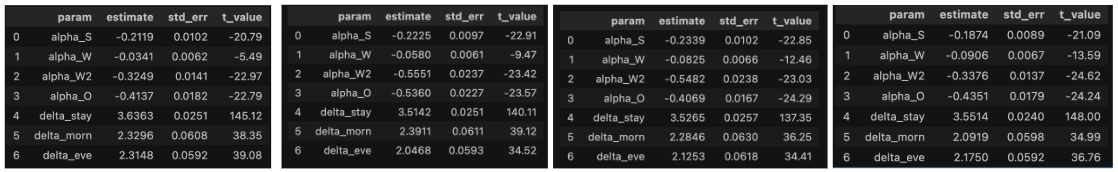
\includegraphics[width=\linewidth]{assets/behavior_modeling/column3/ABMS07.png}
  \captionof{figure}{RLモデルによる時期の比較}
  \label{fig:label-of-this-figure}
\end{center}

\textbf{実データとRLモデルの整合性}
・全体的にどの時期のデータについても推定精度は高い
・4つ全ての時期のデータについて、H在宅を0.5h程度高く見積もる傾向があった
・4つ全ての時期のデータについて、W通勤・仕事を0.5h程度低く見積もる傾向にあった
・S買い物、W2業務とOその他については極めて高い精度で予測できていた

\begin{center}
  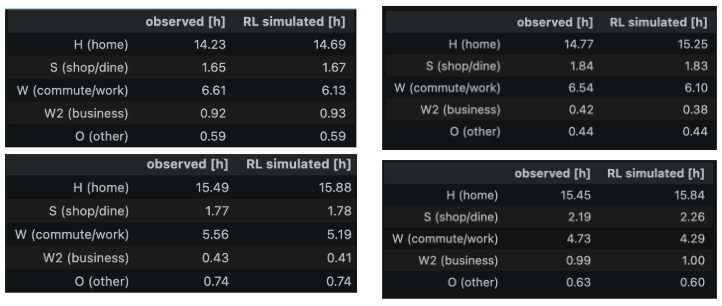
\includegraphics[width=\linewidth]{assets/behavior_modeling/column3/ABMS08.png}
  \captionof{figure}{RLモデルによる時期の比較}
  \label{fig:label-of-this-figure}
\end{center}

\subsubsection{MDCEVモデルのforecast}
Bhat(2008)のForecasting Algorithm（決定論的最適配分）
・MDCEVモデルではW(通勤，仕事)を多く見積もる傾向がある．
・RLモデルの方がS,W2,Oの活動時間を正確に見積もることができている．

\begin{center}
  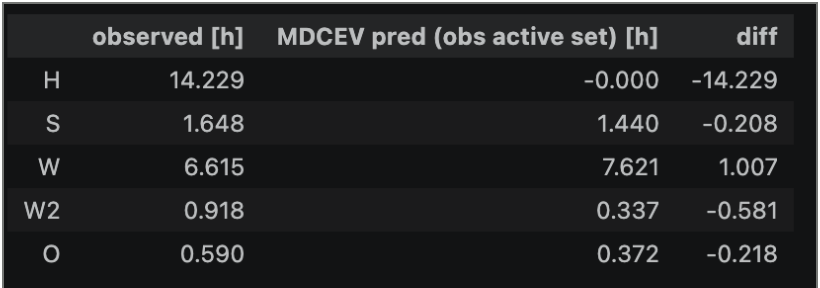
\includegraphics[width=\linewidth]{assets/behavior_modeling/column3/ABMS09.png}
  \captionof{figure}{実データとRLデータの整合性}
  \label{fig:label-of-this-figure}
\end{center}

\begin{center}
  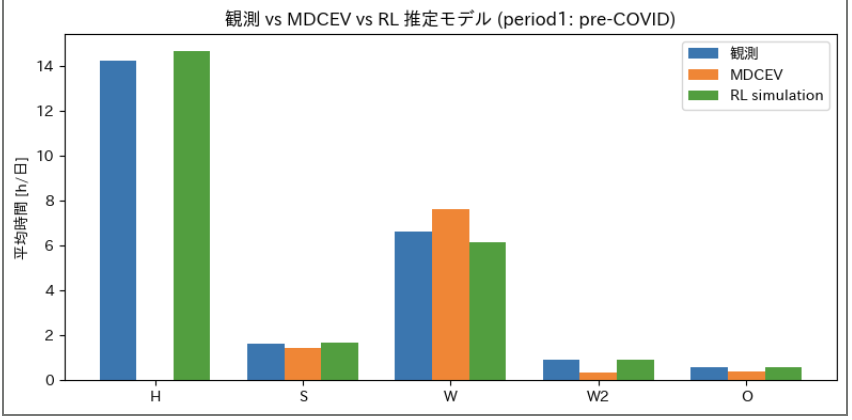
\includegraphics[width=\linewidth]{assets/behavior_modeling/column3/ABMS10.png}
  \captionof{figure}{実データとRLデータの整合性}
  \label{fig:label-of-this-figure}
\end{center}

\subsubsection{Day-to-Day Dynamics}
通常のRecursive Logit modelでは，過去の活動履歴を考慮することはできないが，ここに
\textbf{全ての活動に対して同じパラメータを追加する場合}
1日の各活動の最後に行った日からの経過日数も考慮に入れる．
\begin{equation}
U_t(i \to j) = [\text{baseline}] + \theta_{\text{rec}} \cdot \text{recency}_u(a(j))
\end{equation}

\begin{center}
  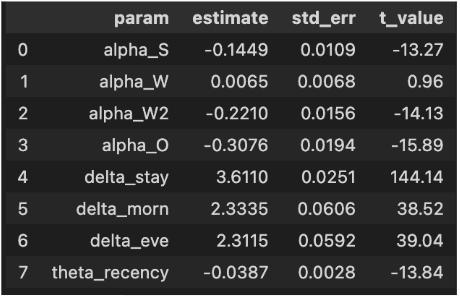
\includegraphics[width=\linewidth]{assets/behavior_modeling/column3/ABMS11.png}
  \captionof{figure}{キャプション}
  \label{fig:label-of-this-figure}
\end{center}
\theta_{\text{rec}} < 0
より，普段やらない活動は将来も選ばれにくい傾向にあるといえる．
recencyを入れた方が，Wの時間については正確に推定することができていた．

\begin{center}
  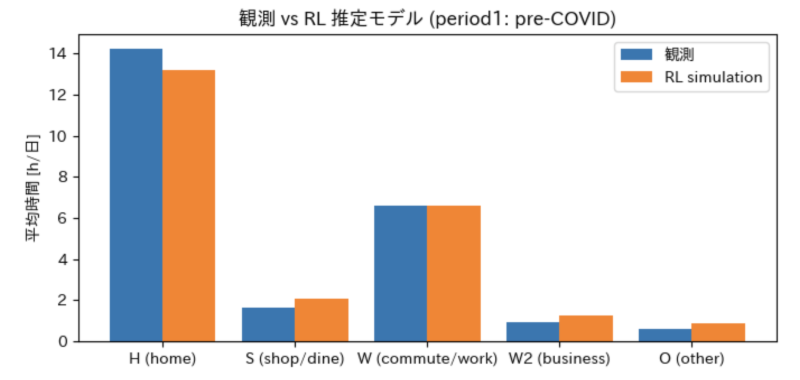
\includegraphics[width=\linewidth]{assets/behavior_modeling/column3/ABMS12.png}
  \captionof{figure}{キャプション}
  \label{fig:label-of-this-figure}
\end{center}


\textbf{活動種類ごとのDay-to-Day Recencyを導入する場合}
活動ごとの個別のパラメータの導入を行い、各活動ごとに違いを見た
レコードごとに効用が異なるのでN個の異なる効用関数を解くことで一人一人の現在の状況に合わせた将来予測を計算

\begin{center}
  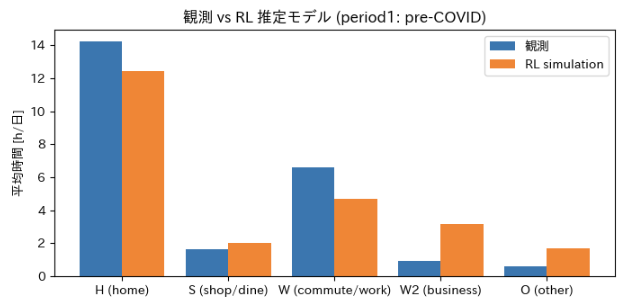
\includegraphics[width=\linewidth]{assets/behavior_modeling/column3/ABMS13.png}
  \captionof{figure}{キャプション}
  \label{fig:label-of-this-figure}
\end{center}

モデルのはまり具合は悪化してしまったが，これはW(business)は他の活動と比べて，発生頻度が低いため，負の相関を強く見積り過ぎた結果，シミュレーション上ではW2が過剰に選ばれる事態が発生してしまったのではないかと考えられる．
さらに，サンプル数が少ないため，個人の極端な行動の影響を受けている可能性が高い．

）
\end{column}
\clearpage
\input{chapters/behavior_modeling/ch5-estimation}

\addcontentsline{toc}{section}{参考文献}
\bibliographystyle{stone-ship}
\bibliography{../src/bibliography/behavior_modeling}

\chapter{最適化}
\chapterauthor{今村啓太}
\section{最適化とは}

\subsection{最適化の基本的な考え方}

私たちは日常生活の中で，意識するかどうかにかかわらず，常に何らかの選択を行っている．例えば，大学へ行くときにどの経路を通れば最も早く到着できるかを考えることがあるし，限られた時間の中でどの作業から先に進めるべきかを判断することもある．また，企業であれば，複数の工場の中でどこにどれだけ生産を割り当てれば費用を最も小さくできるかを考えるし，物流事業者であれば，複数の配送先をどの順番で回れば移動距離を最も短くできるかを検討する．このように，いくつかの選択肢の中から，ある基準に照らして最も望ましいものを選ぶという考え方は，社会のさまざまな場面に現れている．

最適化とは，このような「最も良い選択」を，感覚や経験だけではなく，明確な基準と制約のもとで数理的に求めようとする考え方である．何を良いとみなすかは，問題の目的によって異なる．例えば，移動であれば時間が短いことが望ましいかもしれないし，輸送であれば費用が小さいことが重視されるかもしれない．場合によっては，安全性や公平性，環境負荷の低さなどが重視されることもある．したがって，最適化とは答えを計算する作業ではなく，まず何を評価したいのかを明確にし，そのうえで何が可能で何が不可能なのかを整理する作業でもある．

また，最適化は，図\ref{fig:1_frame}に示すように現実社会の課題を解決するための体系的なアプローチとして位置づけられる\cite{Anai2015}．すなわち，まず現実社会に存在する問題を整理し（課題の把握），それを数理モデルとして定式化することで扱いやすい形に落とし込む．次に，そのモデルに対して最適化計算を行い，最適解を導出する．さらに，得られた解について分析を行い，現実の状況に適用可能かを確認することで，具体的な解決施策へとつなげていく．このように最適化は，「課題の理解→定式化→解の導出→検証・適用」という一連のプロセスを通じて，現実の意思決定を支援する重要な枠組みである．

%\includegraphics[width=0.8\textwidth]{assets/demand/my-figure.png}

\begin{figure}[t]
\centering
\includegraphics[width=0.8\textwidth]{assets/optimization/optimization/1_opt.pdf}
\caption{最適化による課題解決のフレーム}
\label{fig:1_frame}
\end{figure}

\subsection{最適化問題の数学的定式化}
最適化問題は一般に次のように書かれる．
\begin{align}
\text{minimize}\quad&f(x)\\\
\text{subject to}\quad&x\in X
\end{align}
ここで，$x$は決定変数と呼ばれ，私たちが選ぶ対象を表している．$f(x)$は目的関数と呼ばれ，その選択がどれだけ良いか，あるいはどれだけ悪いかを数値として表したものである．どのような選択が望ましいのかを数量的に評価するためのものが目的関数である．

また，$x\in X$は制約条件を表している．ここで，$X$は実行可能集合と呼ばれ，満たすべき条件をすべて満たすような$x$の集合である．例えば，資源の上限や容量制約，順序や論理関係など，現実の問題における制限はこの集合$X$によって表現される．

このように，決定変数，目的関数，制約条件を組み合わせることで，最適化問題は一つの数理モデルとして定式化される．目的関数や制約条件に何を含めるかによって，得られる解の意味は大きく変わる．例えば，移動時間だけを目的関数に含めれば，費用や環境負荷は考慮されないことになる．逆に，制約を増やしすぎれば，現実には解けないほど複雑なモデルになってしまうこともある．したがって，最適化においてはどのように問題を表現するかが重要である．本書で扱うさまざまな問題も，この観点から理解することが重要である．

\subsection{最大化問題と最小化問題}

最適化問題には，大きく分けて，何かをできるだけ大きくしたい問題と，何かをできるだけ小さくしたい問題の二種類がある．前者は最大化問題，後者は最小化問題と呼ばれる．例えば，利益や満足度，利便性などを大きくしたい場合には最大化問題となる．一方で，費用，時間，損失，移動距離などを小さくしたい場合には最小化問題となる．
ある関数$f(x)$を最大化する問題は，その符号を反転させた$-f(x)$を最小化する問題として書き直すことができる．すなわち，
\begin{equation}
\max f(x)
\end{equation}
という問題は，
\begin{equation}
\min \{-f(x)\}
\end{equation}
と等価である．したがって，理論的には最大化と最小化を厳密に区別する必要はなく，どちらか一方に統一して議論することができる．本書では，記述を簡潔にするため，主として最小化問題の形で説明を行う．

ただし，ここで重要なのは，最大化か最小化かという表面的な違いではなく，何を評価対象としているかである．例えば，ある物流問題において「利益最大化」と「費用最小化」は似た意味を持つかもしれないが，必ずしも同じではない．利益は収入から費用を差し引いたものであり，費用だけを最小化しても利益が最大になるとは限らないからである．

また，現実の問題では，評価したいものが一つだけとは限らない．例えば，都市交通では，移動時間を短くしたい一方で，費用も抑えたいし，環境負荷も小さくしたいというように，複数の目的が同時に存在することが多い．このような問題では，複数の目的をどう統合するかが新たな課題となる．例えば，時間と費用を重み付き和として
\begin{equation}
f(x)=\alpha T(x)+\beta C(x)
\end{equation}
のように表し，一つの目的関数として扱うことがある．ここで，$T(x)$は時間，$C(x)$は費用，$\alpha ,\beta $はそれぞれの重要度を表す重みである．このような考え方は，多目的最適化となる．

このように，最大化問題と最小化問題は数学的には容易に変換できるが，目的関数に何を含めるかは決して自明ではない．したがって，「最大化か最小化か」という形式だけに注目するのではなく，その目的関数が何を意味しているのか，どのような価値判断を反映しているのかを意識して読むことが大切である．

\subsection{連続最適化と離散最適化}

最適化問題は，決定変数がどのような値をとるかによって，大きく連続最適化と離散最適化に分けられる．この区別は，問題の性質，理論，解法のすべてに大きな影響を与える．

連続最適化とは，決定変数が連続的な値，すなわち実数値をとる最適化問題である．例えば，生産量，速度，時間，投資割合のように，理論上は小数点以下を含む任意の値をとることができる変数を扱う問題がこれに該当する．変数$x$が実数全体，あるいはその一部の区間に属するとき，これを記号で
\begin{equation}
x\in \mathbb{R}^n
\end{equation}
のように表す．このような問題では，目的関数や制約関数がなめらかであれば，微分や勾配といった解析的な手法を用いて解を探すことができる．

例えば，単純な問題として，関数
\begin{equation}
f(x)=x^2
\end{equation}
を最小にする$x$を考える．この関数は放物線であり，$x=0$のとき最小値$0$をとる．微分を用いれば，
\begin{equation}
\frac{d}{dx}f(x)=2x
\end{equation}
であるから，これが$0$となる点，すなわち$x=0$が候補となる．このように，連続最適化では，関数の局所的な変化率に関する情報を使って最適解を見つけることができる．後に学ぶ最適性条件やKKT条件は，まさにこの考え方を一般化したものである．

これに対して，離散最適化では，決定変数は飛び飛びの値しかとらない．例えば，ある道路を使うか使わないかという選択は，通常，0か1で表される．また，複数の配送先をどの順番で回るかという問題では，順序そのものが変数となる．このような問題では，変数は整数や0--1値として表される．例えば，0--1変数であれば，
\begin{equation}
x_{ij}\in \{0,1\}
\end{equation}
のように表される．

離散最適化が難しい理由の一つは，連続最適化のように微分を使うことができない点にある．変数が0か1しかとらないのであれば，「少しだけ増やす」という概念自体が意味を持たないからである．さらに本質的な難しさは，可能な解の数が急速に増加することにある．例えば，$n$個の地点を一度ずつ訪問する順序を考えると，その候補数は$n!$通りある．$n=5$であれば$5!=120$通りで済むが，$n=10$では$10!=3,628,800$通りとなり，$n=20$ではその数は天文学的な大きさになる．これがいわゆる組合せ爆発であり，巡回セールスマン問題や配送計画問題が難しいとされる主な理由である．

連続最適化と離散最適化の違いは，解法にもはっきりと現れる．連続最適化では，単体法，内点法など，関数の構造を利用した方法が有効である．一方で，離散最適化では，分枝限定法，列生成法など，離散的な選択肢をうまく探索する方法が中心となる．

ただし，現実の問題は必ずしもこの二つのいずれかにきれいに分かれるわけではない．むしろ，両者が混在する場合のほうが多い．例えば，車両配送の問題では，ある顧客を訪問するかどうかは0--1変数で表される一方，到着時刻や待ち時間は連続変数で表されることが多い．このような問題は混合整数計画問題と呼ばれ，連続最適化と離散最適化の両方の性質を併せ持つ．

したがって，最適化を学ぶ際には，まず自分が扱っている変数が連続なのか離散なのかを見極めることが重要である．この違いを正しく理解することで，なぜ問題によって必要な理論やアルゴリズムが異なるのかが見えてくる．

\subsection{実行可能領域と最適解}

最適化問題を理解するうえで，実行可能領域と最適解という二つの概念は中心的な役割を果たす．これらをきちんと理解しないまま解法だけを学ぼうとすると，なぜその手法が成り立つのか，なぜある問題は解きやすく別の問題は解きにくいのかが見えにくくなる．

まず，実行可能領域とは，与えられた制約条件をすべて満たす解の集合のことである．例えば，二変数$x_1,x_2$に対して
\begin{equation}
x_1+x_2\le q4,\qquad x_1\ge q0,\qquad x_2\ge q0
\end{equation}
という制約があるとする．このとき，これらの条件を同時に満たすすべての点$(x_1,x_2)$の集まりが実行可能領域である．図で描けば，第一象限内のある三角形領域になる．

この実行可能領域の中で，目的関数を最大（または最小）にする点が最適解である．数式で書けば，$x^*$が最適解であるとは，
\begin{equation}
f(x^*)\leq f(x)\qquad\text{for all}x\in X
\end{equation}
が成り立つことを意味する．ここで$X$は実行可能領域である．つまり，最適解とは，実行可能なすべての候補の中で最も優れた解である．

ただし，ここで注意しなければならないのは，「最適」という言葉には局所的な意味と大域的な意味があるということである．ある点$a$の近くを少し動かしてもそれより良い解が見つからない場合，その点を局所的最適解と呼ぶ（図\ref{fig:1_best}）．一方，実行可能領域全体を見渡して，それ以上良い解が存在しない場合，その点を大域的最適解と呼ぶ．連続最適化では，局所最適解はしばしば勾配が0になる点として現れるが，それが必ずしも大域最適解とは限らない．

\begin{figure}[t]
\centering
\includegraphics[width=0.8\textwidth]{assets/optimization/optimization/1_best.pdf}
\caption{局所的最適解と大域的最適解}
\label{fig:1_best}
\end{figure}

例えば，非凸な関数では，複数の谷が存在することがある．その場合，ある谷の底に到達したとしても，もっと深い別の谷が離れた場所にあるかもしれない．局所的最適解と大域的最適解の違いは，まさにこのような状況に対応している．

ここで重要になるのが凸性である．実行可能領域$X$が凸集合であるとは，$X$の任意の二点$x,y$をとったとき，それらを結ぶ線分上のすべての点も$X$に含まれることを意味する．数式で書けば，任意の$\lambda\in [0,1]$に対して
\begin{equation}
\lambda x+(1-\lambda)y\in X
\end{equation}
が成り立つことである．さらに，目的関数$f(x)$も凸関数であれば，その問題は凸最適化問題となる．このとき，局所最適解は必ず大域最適解になる．これは最適化理論において最も重要な性質の一つであり，なぜ凸最適化が特別に重視されるのかを説明している．

また，最適解は常に一つとは限らない．例えば，線形計画問題では，目的関数の等高線が実行可能領域の辺と平行になる場合，その辺上のすべての点が最適解になることがある．このように，複数の最適解が存在する場合には，目的関数の値だけでは解が一意に定まらない．その場合，別の基準，例えば公平性や実務上の扱いやすさなどを追加して，最終的な解を選ぶことがある．

このように，実行可能領域と最適解の概念は，最適化問題の土台をなしている．制約がどのような形で実行可能領域を作り，その中で目的関数がどのように最適解を決めるのかを理解することは，後に学ぶ双対性やアルゴリズムの理解にも直結する．

\begin{example}[title={クイズ1：バス運行計画はどのタイプの最適化？}]
ある都市において，バス路線の運行計画を最適化する問題を考える．具体的には，各路線の運行頻度や経路を決定し，利用者の総移動時間の短縮と運行コストの削減，さらに環境負荷の低減を同時に考慮する．また，バスは各停留所を必ずしもすべて通過する必要はなく，運行経路の選択や停車の有無も意思決定の対象とする．

この問題に関する次の記述のうち，本文の内容として最も適切なものはどれか．

\begin{itemize}
\item[(ア)]
この問題は移動時間やコストといった連続量を扱うため連続最適化として定式化される．また，目的関数に複数の指標を含める場合でも，それらは単純に加算することで統一的に扱えるため，評価対象の選び方が解の意味に与える影響は限定的である．さらに，最大化問題として定式化する場合には最小化問題とは異なる理論体系を用いる必要がある．

\item[(イ)]
この問題では，運行頻度や時間は連続的に扱われる一方で，経路の選択や停車の有無は離散的な意思決定となるため，連続最適化と離散最適化の性質が混在する．また，移動時間・コスト・環境負荷といった複数の評価指標は重み付けなどにより統合されることがあるが，その設定によって解の意味は変わり得る．さらに，最大化問題と最小化問題は数学的には変換可能であるが，何を目的関数として表現するかは問題の本質に関わる．

\item[(ウ)]
この問題では，停車の有無や経路選択といった離散的な意思決定が含まれるため，解の候補数が非常に多くなる可能性がある．そのため，すべての候補を網羅的に探索することは現実的ではなく，何らかの探索戦略を用いることが重要となる．また，実行可能領域が与えられていれば，局所最適解であっても大域的最適解とみなしてよい．
\end{itemize}

\hyperref[ans:bus1]{$\rightarrow$ 正解・解説は節末を参照}
\end{example}

\subsection{線形最適化と非線形最適化}

最適化問題を分類するもう一つの重要な観点は，目的関数や制約条件の形が線形であるか，それとも非線形であるかという点である．この違いは，問題の扱いやすさや理論の美しさに大きく関係している．

線形最適化とは，目的関数と制約条件のすべてが変数に関して一次式で表される最適化問題である．典型的には，次のような形で書かれる．
\begin{align}
\text{minimize}\quad&c^Tx\\
\text{subject to}\quad&Ax\le b
\end{align}
ここで，$x$は変数ベクトル，$c$は目的関数の係数ベクトル，$A$は制約係数行列，$b$は右辺ベクトルである．$c^Tx$は各変数に重みをかけて足し合わせた形であり，$Ax\le b$も各制約が一次不等式で表されている．

線形であることにより，実行可能領域は凸多面体という扱いやすい形になる．そして，このとき最適解はその凸多面体の頂点のいずれかに存在することが知られている．これは直感的には，平面で表される目的関数を一定方向に移動させていくと，最初に接する点が頂点になるという幾何学的な性質に対応している．この構造のおかげで，単体法や内点法のような強力なアルゴリズムが成立する．

% \begin{figure}[t]
% \centering
% \includegraphics[width=0.8\textwidth]{assets/optimization/optimization/1_liner.pdf}
% \caption{線形最適化と非線形最適化}
% \label{fig:1_liner}
% \end{figure}

一方で，目的関数や制約の中に二乗項，積，指数関数，対数関数，三角関数などが含まれる場合，その問題は非線形最適化となる．例えば，
\begin{equation}
f(x)=x^2
\end{equation}
や
\begin{equation}
f(x)=x_1x_2
\end{equation}
のような関数は非線形である．非線形最適化では，線形最適化のような単純な幾何構造は一般には失われる．そのため，最適解を見つけることが急に難しくなる．

非線形最適化で重要なのは，局所最適解と大域最適解が一致しない場合があることである．例えば，
\begin{equation}
f(x)=x^4-x^2
\end{equation}
という関数を考えると，この関数は複数の谷を持つ形をしており，局所的に低い点がいくつか存在する．このような関数では，ある解法が一つの谷の底にたどり着いたとしても，それが全体の中で最も低い点であるとは限らない．これが，非線形最適化，特に非凸最適化の難しさである．

ただし，非線形であっても凸性が保たれていれば，問題はかなり扱いやすくなる．目的関数が凸関数であり，実行可能領域も凸集合である場合，その問題は凸最適化問題と呼ばれる．このとき，任意の局所最適解は大域最適解でもある．これは理論的にも実務的にも重要な性質であり，現代最適化理論の中心をなしている．

都市交通や物流の分野では，現実の現象を忠実に表そうとすると，しばしば非線形性が現れる．例えば，交通量と旅行時間の関係，需要と料金の関係，混雑と効用の関係などは，一般に線形では表しにくい．そのため，実問題では非線形最適化が現れることが多い．しかし一方で，理論や計算のしやすさの観点から，まず線形モデルとして近似し，そのあと必要に応じて非線形性を導入するという進め方もよく行われる．

したがって，線形最適化と非線形最適化の違いを理解することは，その違いが，問題の構造，解の性質，利用できるアルゴリズムの種類にどのような影響を与えるのかを理解することが重要なのである．




\subsection{都市交通における最適化の例}

最適化という考え方は，都市交通や都市物流の分野において重要である．なぜなら，この分野では，限られた道路空間，時間，資源の中で，多数の利用者や車両が相互に影響し合いながら移動しているからである．そこでは常に，何らかの意味で「より良い運用」や「より効率的な配置」が求められている．

最も基本的な例の一つは，最短経路問題である．これは，道路ネットワーク上で出発地から目的地までの距離や時間を最も小さくする経路を求める問題である．道路ネットワークをグラフとして表し，交差点をノード，道路をリンクと考えると，各リンク$(i,j)$に対して移動コスト$c_{ij}$を定め，ある経路の総コストを最小化する問題として定式化できる．

次に，都市物流において中心的な問題となるのが配送計画問題（Vehicle RoutingProble m；VRP）である．この問題では，一つまたは複数の車両が，複数の顧客を訪問して荷物を配送する状況を考える．ここで決めなければならないのは，どの車両がどの顧客を担当するか，そして各車両がどの順序で顧客を訪問するかである．総移動距離や総配送時間を最小化したい一方で，各顧客はちょうど一度訪問されなければならず，各車両の容量制約も守らなければならない．このように，VRPは複数の制約の下で訪問順序を決める組合せ最適化問題であり，都市物流の効率化を考えるうえで不可欠なモデルである．

さらに，どこに物流拠点や駐車場を配置すべきかという施設配置問題も重要である．これは，都市空間の中でどの位置に拠点を置けば，全体として利用者へのアクセス性や配送効率が高くなるかを考える問題であり，長期的な都市計画とも密接に関わっている．



\begin{example}[title={クイズ1 正解・解説}]
\phantomsection\label{ans:bus1}
\textbf{正解：（イ）}

本問題では，運行頻度や時間は連続変数である一方，経路選択や停車の有無は離散変数であるため，連続最適化と離散最適化が混在する混合的な問題となる．

また，移動時間・コスト・環境負荷など複数の評価指標は重み付き和などで統合されることがあるが，その重み設定により解の意味は変化する．したがって，目的関数の設計は本質的に重要である．

さらに，最大化問題は符号反転により最小化問題として表現できるため数学的には等価であるが，何を目的として定式化するかは意思決定そのものに関わる重要な問題である．

(ア)は，離散的意思決定の存在を無視している点，および目的関数の重要性を過小評価している点で不適切である．  

(ウ)は前半の「組合せ爆発」や「探索戦略の必要性」は正しいものの，局所最適解と大域最適解を同一視している点が誤りである．この性質は凸最適化においてのみ成立する．

\end{example}

\section{線形計画法}

\subsection{線形計画法とは}

線形計画法は，目的関数と制約条件のすべてが線形で表される最適化問題であり，数理最適化の理論と応用の両面において中心的な役割を果たしてきた．実際，線形計画法は最適化理論の出発点であると同時に，現在でも生産計画，輸送計画，資源配分など，多くの分野で広く用いられている．

線形計画問題は，一般に次のように書かれる．
\begin{align}
\text{minimize}\quad&c^Tx\\
\text{subject to}\quad&Ax\le b\\
&x\ge 0
\end{align}
ここで，$x\in \mathbb{R}^n$は決定変数ベクトル，$c\in \mathbb{R}^n$は目的関数の係数ベクトル，$A\in \mathbb{R}^{m\times n}$は制約係数行列，$b\in \mathbb{R}^m$は右辺ベクトルである．

多くの現実問題が少なくとも近似的には線形モデルとして表現できる．例えば，生産計画では，製品ごとの生産量を変数とし，総利益や総費用を線形に表すことができる．物流計画では，輸送量に比例してコストが増えると仮定すれば，やはり線形な目的関数が得られる．資源配分の問題でも，各活動が一定量の資源を消費し，その活動量に比例して利益や費用が変化するならば，線形計画として自然に定式化できる．このように，完全に厳密ではなくても，「まず線形近似から始める」という考え方は多くの分野で有効である．

また，線形計画問題は幾何学的にも代数的にも美しい構造を持っており，そのため強力な理論とアルゴリズムが成立する．一般の非線形最適化では，局所最適と大域最適が一致しないことや，複数の鞍点が現れることが問題を難しくする．しかし，線形計画では実行可能領域が凸多面体となり，目的関数も線形であるため，問題構造が整理される．その結果，後に見るように，双対問題が自然に定義できる，KKT条件が必要十分条件になる，といった強い性質が得られる．

線形計画法を理解するためには，まず線形性が何を意味しているのかを押さえる必要がある．線形関数とは，変数の一次結合で表される関数であり，
\begin{equation}
f(x)=c_1x_1+c_2x_2+\cdots+c_nx_n
\end{equation}
のような形をしている．ここでは，変数同士の積や二乗項は現れない．したがって，各変数の影響は加法的であり，ある変数を増やしたときの目的関数への寄与は，他の変数の値に依存しない．制約も同様に，
\begin{equation}
a_{i1}x_1+a_{i2}x_2+\cdots+a_{in}x_n\le b_i
\end{equation}
のような一次不等式で表される．この単純さが，後に見る凸性，双対性，単体法などの理論を可能にしている．

\subsection{線形計画問題の幾何学的理解}

線形計画法の本質を理解するうえで，幾何学的な見方は重要である．2変数あるいは3変数の場合には，制約条件を図で表すことができ，そのとき実行可能領域は半平面や半空間の共通部分として得られる．線形不等式で表される集合は凸集合であり，したがって，線形計画問題の実行可能領域は凸多面体となる．この「凸多面体」という性質こそが，線形計画法を特別に扱いやすいものにしている．

例えば，2変数の問題
\begin{align}
\text{minimize}\quad&-x_1-x_2\\
\text{subject to}\quad&x_1+x_2\le 4\\
&x_1\le 3\\
&x_2\le 2\\
&x_1,x_2\ge 0
\end{align}
を考えると，実行可能領域は平面上の多角形として表される．各制約は一つの半平面を表し，その共通部分として，有限個の辺と頂点からなる領域が得られる．一方，目的関数
\begin{equation}
f(x_1,x_2)=-x_1-x_2
\end{equation}
の等高線は，
\begin{equation}
x_1+x_2=\text{const.}
\end{equation}
という直線の族となる．最適化とは，この等高線を一定方向に平行移動させていき，実行可能領域に最後まで接している点を求めることに対応する．

\begin{figure}[t]
\centering
\includegraphics[width=0.8\textwidth]{assets/optimization/optimization/2_contour.pdf}
\caption{線形計画問題における実行可能領域と最適解}
\label{fig:2_contour}
\end{figure}

この説明から分かるように，線形計画法の目的関数は曲面ではなく平面であり，実行可能領域も凸な多面体である．したがって，最適化は「曲がった谷底を探す」作業ではなく，「平面を押し当てていって最後に接する場所を探す」作業とみなせる．このイメージは，非線形最適化と対比すると分かりやすい．非線形最適化では局所的なくぼみや鞍点が現れうるが，線形計画ではそのような複雑さはなく，幾何学的構造が整理されている．

この幾何学的な見方から分かる最も重要な事実は，線形計画問題の最適解は実行可能領域の頂点に存在するということである．厳密には，実行可能領域が空でなく，目的関数が下に有界であるならば，最適解は少なくとも一つの極点で達成される．これは，線形関数が凸多面体の内部で曲がることなく一定方向に変化するため，最小値は境界，さらにいえば頂点に押し出されるからである．

この事実は，線形計画法の理論とアルゴリズムの双方にとって決定的に重要である．もし最適解が一般に領域内部に現れるのであれば，すべての点を連続的に調べる必要があり，問題ははるかに難しくなる．しかし，最適解が頂点に存在するならば，頂点だけを調べればよいという発想が可能になる．もちろん，頂点の数も大きな問題では膨大になりうるが，「連続無限個の候補」ではなく「有限個の頂点」に問題が還元されることの意味は大きい．

また，線形計画では，複数の最適解が存在することもある．これは，目的関数の等高線が実行可能領域のある辺と平行になり，その辺全体で同じ目的関数値をとる場合に起こる．このとき，最適解は一つの頂点に限らず，辺上の無限個の点にわたって存在する．ただし，その場合でも，少なくとも一つの頂点は最適解である．この性質があるからこそ，頂点探索型のアルゴリズムが依然として有効である．

\subsection{標準形と実行可能基底解}

線形計画法では，問題をある決まった形に変換して扱うことが多い．その代表が標準形である．標準形は通常，
\begin{align}
\text{minimize}\quad&c^Tx\\
\text{subject to}\quad&Ax=b\\
&x\ge 0
\end{align}
という形を指す．一見すると，これは先ほどの一般形よりも特殊に見えるかもしれない．しかし，実際には多くの線形計画問題は，適切な変数変換によってこの形に直すことができる．そのため，理論を整理するときには標準形を前提にすると便利である．

もともとの不等式制約は，スラック変数を導入することで等式制約に変換できる．例えば，
\begin{equation}
a_1x_1+a_2x_2\le b
\end{equation}
という制約は，新たな変数$s\ge 0$を導入して
\begin{equation}
a_1x_1+a_2x_2+s=b
\end{equation}
と書ける．この$s$をスラック変数と呼ぶ．スラック変数は，制約にどれだけ余裕があるかを表している．もし制約がちょうど等号で満たされていれば$s=0$であり，まだ余裕があれば$s>0$である．この意味で，スラック変数は制約の緩み具合を可視化する変数でもある．

一方，$\ge $型制約であれば，余剰変数を引くことで等式に直せるし，自由変数がある場合には，正負二つの非負変数の差として表現することができる．したがって，標準形は人工的な形ではあるが，一般性を大きく損なうことなく用いることができる．このように問題を標準形へ揃えることで，線形計画法の理論を統一的に展開できる．

標準形のもとでは，実行可能解の中でも基底解と呼ばれる解が重要になる．行列$A$の列のうち，ランクと同数の列を選んで正則な部分行列を作り，それに対応する変数を基底変数，残りを非基底変数とする．非基底変数を0とおいて基底変数を解いたときに得られる解を基底解と呼ぶ．さらに，その基底解が$x\ge 0$を満たしていれば，それは実行可能基底解である．

この定義は「自由に選ぶ変数」と「制約式によって自動的に決まる変数」を分けて考えている．標準形では等式制約があるため，すべての変数を自由に選べるわけではない．そこで，一部の変数を0に固定し，残りの変数を制約式から解く．その結果得られる特別な解が基底解である．これは代数的な視点から見た頂点の表現といえる．

この実行可能基底解は，幾何学的には実行可能領域の頂点に対応している．したがって，線形計画法の理論では，「頂点」と「実行可能基底解」は本質的に同じ対象を異なる見方で捉えたものと考えることができる．幾何学的には頂点，代数的には実行可能基底解，という二つの見方があることで，問題の理解は大きく深まる．


\begin{example}[title={クイズ2：信号制御}]
ある都市の四差路交差点において，1サイクルの信号運用を設計する問題を考える．
東西方向と南北方向に対して，それぞれ青時間を設定し，交差点全体のサイクル長は一定とする．
また，各方向の青時間には安全上必要な下限制約があり，青時間の総和はサイクル長を超えてはならない．

ここで，車両遅延の評価を単純化し，各方向の総遅延は対応する青時間の一次式で表されるものとする．
したがって，交差点全体の総遅延も，各方向の青時間の線形関数として表される．
このとき，総遅延を最小化する信号設定を求めたい．

この問題に関する次の記述のうち，本文の内容として最も適切なものはどれか．

\begin{itemize}
\item[(ア)]
目的関数と制約条件がいずれも線形であるので，この問題は線形計画問題として表すことができる．
ただし，実行可能領域は連続な点の集まりであるから，最適解を求めるにはその内部も含めて全体を連続的に調べる必要があり，頂点に注目する考え方は本質的ではない．

\item[(イ)]
目的関数と制約条件がいずれも線形であるので，この問題は線形計画問題として表される．
このとき，実行可能領域は線形不等式の共通部分として与えられる凸多面体となる．
また，目的関数は線形関数であるため，最適解は実行可能領域の頂点の一つで達成される．
さらに，目的関数の等高線が実行可能領域のある辺と平行な場合には，その辺上の複数の点が最適解となりうるが，その場合でも少なくとも一つの頂点は最適解である．

\item[(ウ)]
実行可能領域が凸集合であることから，その内部の任意の2点を結ぶ線分上の点も実行可能である．
したがって，線形目的関数の値もその領域内で一定となり，頂点・辺・内部点のいずれを選んでも目的関数値は変わらない．
このため，線形計画問題では最適解を特定の点として議論する必要はない．
\end{itemize}

\hyperref[ans:lp2]{$\rightarrow$ 正解・解説は節末を参照}
\end{example}


\subsection{双対問題}

線形計画法におけるもう一つの極めて重要な概念が双対性である．ある線形計画問題に対して，それと対をなす別の線形計画問題を定義することができる．もとの問題を主問題，対応して作られる問題を双対問題と呼ぶ\cite{Kanno2012}．

例えば，主問題が
\begin{align}
\text{minimize}\quad&c^Tx\\
\text{subject to}\quad&Ax\ge b\\
&x\ge 0
\end{align}
であるとき，その双対問題は
\begin{align}
\text{maximize}\quad&b^Ty\\
\text{subject to}\quad&A^Ty\le c\\
&y\ge 0
\end{align}
となる．ここで，$y$は双対変数である．この関係を見ると，主問題と双対問題の間には明確な対応があることが分かる．主問題の制約の本数が双対問題の変数の数になり，主問題の変数の数が双対問題の制約の本数になる．また，不等号の向きや最大化・最小化の関係にも一定の規則がある．

双対変数は，各制約に対応する「影の価格」や「限界価値」として解釈される．例えば，ある資源制約に対応する双対変数が大きいならば，その資源を1単位増やしたときの価値が高いことを意味する．言い換えれば，その資源が現在の最適解において希少であり，ボトルネックになっていることを表している．この意味で，双対問題は主問題の背後にある資源配分や価格付けの構造を明らかにしてくれる．

双対性は，線形計画法において美しい形で成立する．まず弱双対性によれば，主問題の任意の実行可能解$x$と双対問題の任意の実行可能解$y$に対して，
\begin{equation}
b^Ty\le c^Tx
\end{equation}
が成り立つ．これは，双対問題の目的関数値が主問題の目的関数値の下界あるいは上界を与えることを意味する．最小化問題と最大化問題がこのような不等式で結ばれているという事実は，重要である．というのも，もしある主実行可能解と双対実行可能解について両者の目的関数値が一致すれば，その瞬間に両者が最適であることが分かるからである．

さらに，強双対性によれば，適当な条件のもとで主問題と双対問題の最適値は一致する．すなわち，
\begin{equation}
c^Tx^*=b^Ty^*
\end{equation}
が成り立つ．この事実は，線形計画法を特別なものにしている核心である．なぜなら，主問題を直接見るだけでは分からない最適性を，双対問題を通じて理解できるからである．また，最適解の意味を「変数の値」だけでなく「資源の価値」という別の視点から捉えられるようになる．

後に学ぶ列生成法では，双対価格を用いて新しい列の有用性を判定する．ベンダーズ分解では，部分問題の双対情報がカットとして主問題へ返される．さらに，ネットワーク最適化や資源配分問題でも，双対変数の経済的意味づけは極めて重要である．したがって，双対問題の導入は，線形計画法の理解を深めるだけでなく，後続の多くの手法の基礎を与えるものである．

\subsection{KKT条件と相補性条件}

最適化問題において，「この解が本当に最適か？」を判定するための条件として，KKT条件（Karush--Kuhn--Tucker条件）がある．これは，不等式制約を含む問題に対する最適性条件であり，ラグランジュの未定乗数法を拡張したものである．

一般に，次のような問題を考える：
\begin{align}
\text{minimize}\quad&f(x)\\
\text{subject to}\quad&g_i(x)\le 0\quad(i=1,\dots,m)\\
&h_j(x)=0\quad(j=1,\dots,p)
\end{align}

このとき，適当な条件のもとで，最適解$x^*$は次の4つの条件（KKT条件）を満たす：

\begin{itemize}
\item [(1)]停留条件
「目的関数と制約をすべて考慮したとき，これ以上改善できない状態」
\begin{equation}
\nabla f(x^*)+\sum_{i=1}^m\lambda_i\nabla g_i(x^*)+\sum_{j=1}^p\mu_j\nabla h_j(x^*)=0
\end{equation}

\item [(2)]実行可能性
「もとの制約を満たしている」
\begin{equation}
g_i(x^*)\le 0,\quad h_j(x^*)=0
\end{equation}

\item [(3)]双対実行可能性
「不等式制約に対応する係数（ラグランジュ乗数）は負にならない」
\begin{equation}
\lambd a_i\ge 0
\end{equation}

\item [(4)]相補性条件
\begin{equation}
\lambda_i\,g_i(x^*)=0
\end{equation}
\end{itemize}

特に重要なのが，相補性条件である．これは，制約に余裕があるなら，その制約は最適解に影響していない
ということを表している．

実際，相補性条件$\lambda_ig_i(x^*)=0$は，次のどちらかが必ず成り立つことを意味する：

\begin{itemize}
\item 制約に余裕がある（$g_i(x^*)<0$）$\Rightarrow$$\lambda_i=0$
\item ラグランジュ乗数が正（$\lambda_i>0$）$\Rightarrow$制約はぴったり効いている（$g_i(x^*)=0$）
\end{itemize}

つまり，
「効いている制約（境界にある制約）だけが最適解を決める」
という構造になっている．

この考え方は重要であり，例えば線形計画では，
最適解は「いくつかの制約がちょうど等号になる点（＝頂点）」に現れるが，
これはまさに相補性条件の直感と一致している．

さらに，線形計画のような凸最適化問題では，KKT条件は必要条件ではなく十分条件にもなる．
したがって，
KKT条件を満たす解を見つける$\;\Longle ftrightarrow\;$最適解を見つける
という強い性質が成り立つ．

\subsection{双対性とKKT条件の関係}

KKT条件は，線形計画法において簡潔な形で現れる．線形計画問題は凸最適化問題であるため，KKT条件は最適性の必要条件であるだけでなく十分条件でもある．つまり，KKT条件を満たす点は最適解である．この点は，線形計画法が理論的に扱いやすい理由の一つである．

線形計画におけるKKT条件を見れば，停留条件はまさに主問題と双対問題の制約に対応し，相補性条件は主変数と双対変数の間の関係を表している．この相補性条件は，相補スラックネスと呼ばれ，線形計画における最適性の判定条件として重要である．例えば，制約に余裕があるならば対応する双対変数は0であり，双対変数が正ならば対応する制約はちょうど等号で成立していなければならない．この関係は，KKT条件の一般形を最も分かりやすく具体化したものといえる．

少し丁寧に見るために，主問題を
\begin{align}
\text{minimize}\quad&c^Tx\\
\text{subject to}\quad&Ax\ge b\\
&x\ge 0
\end{align}
とし，双対問題を
\begin{align}
\text{maximize}\quad&b^Ty\\
\text{subject to}\quad&A^Ty\le c\\
&y\ge 0
\end{align}
とする．このとき，相補スラックネスは概念的には，
\begin{equation}
y_i\bigl((Ax-b)_i\bigr)=0
\end{equation}
および
\begin{equation}
x_j\bigl((c-A^Ty)_j\bigr)=0
\end{equation}
のような形で表される．これは，主問題側で余裕のある制約には双対変数がつかず，双対問題側で余裕のある制約には主変数が正にならないことを意味する．

この関係を経済的に解釈すると分かりやすい．ある資源制約にまだ余裕があるならば，その資源は追加しても価値がないので，双対価格は0になる．逆に，双対価格が正であるならば，その資源はちょうど使い切られており，1単位増やすことに価値がある．このように，相補スラックネスは「余っている資源には価格がつかず，価値のある資源は使い切られている」という直感を表している．

また，KKT条件と双対性の関係を理解すると，最適性判定の考え方が明確になる．主問題の実行可能解と双対問題の実行可能解を一つずつ持ってきて，さらに相補スラックネスが成り立っていれば，その二つはともに最適解である．これは，弱双対性による上下界の関係と，KKT条件による局所的な整合条件とが，線形計画法では一つに統合されていることを意味している．

したがって，双対性とKKT条件の関係を理解することは，「最適性とは何か」を深く理解することにつながる．また，後に学ぶ列生成法やベンダーズ分解では，双対解がアルゴリズムの中で直接使われるため，ここで相補スラックネスや双対変数の意味をしっかり理解しておくことが重要である．


\begin{example}[title={クイズ3：双対性による最適性判定}]
ある都市の道路ネットワークにおいて，各リンクの交通流量（台/時）を連続変数とし，
総走行コストを最小化する線形計画問題を考える．
各リンクには容量制約があり，それを超えないように流量を決定する．

あるとき，この主問題に対して，
実行可能な解 $x$ と，対応する双対問題の実行可能解 $y$ が得られたとする．
それぞれの目的関数値を計算したところ，
\[
c^T x = b^T y
\]
が成り立っていることが確認された．

この状況に関する次の記述のうち，本文の内容として最も適切なものはどれか．

\begin{itemize}
\item[(ア)]
主問題と双対問題の目的関数値が一致していても，
それぞれが最適解であるとは限らない．
最適性を判定するためには，
さらに別の条件を確認する必要がある．

\item[(イ)]
主問題と双対問題の目的関数値が一致しているので，
弱双対性によりこの関係は常に成立する．
したがって，この一致から最適性について特別な結論を導くことはできない．

\item[(ウ)]
主問題と双対問題の実行可能解に対して目的関数値が一致しているので，
それらはともに最適解である．
\end{itemize}

\hyperref[ans:dual4]{$\rightarrow$ 正解・解説は節末を参照}
\end{example}



\subsection{代表的な解法}

線形計画問題は凸多面体構造を持つため，
その幾何学的性質を活かした効率的な解法が存在する．
ここでは，代表的な解法である単体法と内点法について，
その基本的な考え方と特徴を詳しく説明する．

\subsubsection{単体法}

単体法は，線形計画問題の最適解が実行可能領域の頂点に存在するという性質に基づくアルゴリズムである．
基本的な考え方は，ある実行可能基底解（頂点）から出発し，
隣接する頂点へと移動しながら目的関数値を改善していくことである．

標準形
\begin{align}
\text{minimize}\quad&c^Tx\\
\text{subject to}\quad&Ax=b\\
&x\ge 0
\end{align}
を考えると，基底変数と非基底変数に分けることで，
基底解が定まる．単体法では，非基底変数のうち，
目的関数を改善する方向に寄与するものを選び（入る変数），
対応して基底変数の一つを外す（出る変数）ことで，
新しい基底解へと移動する．

この操作はピボット操作と呼ばれ，
基底の更新として代数的に実行される．
幾何学的には，これは多面体の辺に沿って隣接する頂点へ移動する操作に対応している．

単体法の重要な特徴は，
\begin{itemize}
\item 常に実行可能解を保ちながら探索を行う
\item 各ステップで目的関数値が単調に改善される
\end{itemize}
という点である．

また，最適性の判定は，
すべての非基底変数に対して改善方向が存在しないこと，
すなわち還元コストが非負であることによって行われる．
この条件は双対問題の実行可能性とも対応しており，
単体法は主問題と双対問題を同時に満たす方向へ進んでいると解釈できる．

理論的には，単体法は最悪の場合指数時間を要することが知られているが，
実務上は高速に収束することが多く，
長年にわたり広く用いられてきた．

\begin{figure}[t]
\centering
\includegraphics[width=0.8\textwidth]{assets/optimization/optimization/2_simplex.pdf}
\caption{単体法と内点法}
\label{fig:2_simple x}
\end{figure}

\subsubsection{内点法}

内点法は，単体法とは異なり，
実行可能領域の内部を通る経路をたどって最適解に近づくアルゴリズムである．

基本的な考え方は，
不等式制約を直接扱う代わりに，
境界に近づくことを抑制するバリア関数を目的関数に加えた問題を解くことである．
例えば，非負制約$x_i>0$に対しては，
\begin{equation}
-\mu\sum_i\log x_i
\end{equation}
のような対数バリア関数を導入する．

すると，元の問題は
\begin{equation}
\min \;c^Tx-\mu\sum_i\log x_i
\end{equation}
のような補助問題に置き換えられる．
ここで，$\mu$を徐々に小さくしていくことで，
解は境界に近づき，最終的に元の線形計画問題の最適解へ収束する．

内点法では，各反復において，
この補助問題の最適性条件（KKT条件）を解くことで，
解を更新していく．
特に，ニュートン法に基づく方向を用いて，
効率的に中心経路（centralpath）に沿って移動する．

単体法との大きな違いは，
\begin{itemize}
\item 頂点ではなく内部の点を通る
\item 各反復で連続的に解を更新する
\end{itemize}
という点である．

理論的には，内点法は多項式時間で解けることが示されており，
特に大規模かつ疎な問題に対して高い性能を発揮する．
また，数値的に安定であるという利点もある．



\subsection{線形計画法の例}

ここでは，線形計画法がどのように現実問題に適用されるかを理解するために，代表的な二つの問題である輸送問題と生産計画問題を示す．

\subsubsection{輸送問題}

複数の供給地と需要地の間で物資を輸送する問題を考える\cite{hitchcock}．供給地$i$の供給量を$a_i$，需要地$j$の需要量を$b_j$，供給地$i$から需要地$j$への単位輸送コストを$c_{ij}$とする．

変数$x_{ij}$を「供給地$i$から需要地$j$に輸送する量」とすると，問題は次のように定式化される：

\begin{align}
\text{minimize}\quad&\sum_{i}\sum_{j}c_{ij}x_{ij}\\
\text{subject to}\quad
&\sum_{j}x_{ij}=a_i\quad(\for all i)\\
&\sum_{i}x_{ij}=b_j\quad(\for all j)\\
&x_{ij}\ge 0
\end{align}

第1の制約は各供給地の供給量を使い切ることを表し，第2の制約は各需要地の需要を満たすことを表している．この問題はネットワーク構造を持つ線形計画問題の典型例であり，物流やサプライチェーン設計で広く用いられる．

\begin{figure}[t]
\centering
\includegraphics[width=0.8\textwidth]{assets/optimization/optimization/2_trans.pdf}
\caption{輸送問題}
\label{fig:2_trans}
\end{figure}

\subsubsection{生産計画問題}

複数の製品を生産する際に，限られた資源をどのように配分するかを決める問題を生産計画問題という\cite{GELDERS1981101}．製品$j$の生産量を$x_j$，単位利益を$c_j$，資源$i$の利用可能量を$b_i$，製品$j$が資源$i$を消費する量を$a_{ij}$とする．

このとき，総利益を最大化する問題は次のように書ける：

\begin{align}
\text{maximize}\quad&\sum_{j}c_jx_j\\
\text{subject to}\quad
&\sum_{j}a_{ij}x_j\le b_i\quad(\for all i)\\
&x_j\ge 0
\end{align}

ここで，各制約は資源制約を表している．例えば労働時間，原材料，設備能力などがこれに対応する．双対変数は，これらの資源の「限界価値（影の価格）」として解釈できる．

この問題は，企業の生産計画だけでなく，エネルギー供給，交通容量配分，都市物流における資源配分など，多様な分野で基本モデルとして用いられている．


\begin{example}[title={クイズ2 正解・解説}]
\phantomsection\label{ans:lp2}
\textbf{正解：（イ）}

この問題では，各方向の青時間が変数であり，総遅延はそれらの一次式として表されている．
また，サイクル長制約や各方向の下限制約も線形である．
したがって，この問題は目的関数と制約条件がともに線形で与えられる線形計画問題である．

線形計画問題では，実行可能領域は線形不等式の共通部分として与えられるため，凸多面体となる．
さらに，目的関数も線形であるため，最小値は実行可能領域の頂点の少なくとも一つで達成される．
この「最適解は頂点に存在する」という性質が，線形計画法の理論や単体法のようなアルゴリズムの基礎になっている．

また，複数の最適解が存在する場合もある．
たとえば，目的関数の等高線が実行可能領域のある辺と平行であれば，その辺上のすべての点が同じ目的関数値をとる．
しかし，その場合でも少なくとも一つの頂点は最適解に含まれる．

(ア)が誤りである理由は，実行可能領域が連続集合であっても，線形計画問題では最適解を頂点に限定して考えられるという重要な性質を見落としている点にある．
実行可能領域全体を「内部も含めて一様に調べる必要がある」という理解は，線形計画法の本質を外している．

(ウ)が誤りである理由は，凸集合であることと，目的関数値が領域全体で一定であることを混同している点にある．
凸性が意味するのは，「実行可能な2点を結ぶ線分上の点も実行可能である」という幾何学的性質であって，目的関数値が同一になることではない．
線形目的関数は実行可能領域上で一定とは限らず，方向に応じて増減する．
そのため，最適解をどこで達成するかは重要な問題であり，頂点・辺・内部点を区別して考える必要がある．

\end{example}


\begin{example}[title={クイズ3 正解・解説}]
\phantomsection\label{ans:dual4}
\textbf{正解：（ウ）}

この問題の本質は，双対性を用いた最適性判定である．

線形計画問題では，弱双対性により，
任意の主問題の実行可能解 $x$ と双対問題の実行可能解 $y$ に対して，
\[
b^T y \le c^T x
\]
が成り立つ．
これは，双対問題の目的関数値が主問題の目的関数値の下界を与えることを意味する．

ここで，
\[
c^T x = b^T y
\]
が成立しているということは，
この不等式が等号で成立していることを意味する．

したがって，
これ以上目的関数値を改善する余地はなく，
$x$ と $y$ はそれぞれ主問題と双対問題の最適解である．
これは強双対性の帰結であり，
線形計画法における最も重要な最適性判定の一つである．

(ア)は，等号成立の意味を理解しておらず誤りである．

(イ)は，弱双対性を誤解している．
弱双対性は不等式を保証するものであり，
等号が成立することは特別な状況であり，
最適性を示す強い条件である．

\end{example}

\clearpage
\begin{column}{ミニ研究}
（担当者：桑本）
\end{column}
\clearpage

\section{組合せ最適化の基礎}
\subsection{組合せ最適化とは}

最適化問題の中でも，変数が離散的な値をとる問題を，総称して組合せ最適化という．組合せ最適化では，変数は一般に0--1変数，整数，集合などとして表される．多数の離散的な候補の中から，ある制約のもとで最も良い組合せを選ぶ問題である．

ここで「組合せ」という言葉は，いくつかの要素を選ぶという意味に限らない．実際には，ある集合から要素を選ぶ問題もあれば，要素の並べ方を決める問題もあり，また，複数の対象をどのように割り当てるかを決める問題もある．例えば，目的地までの経路を決める問題では，どの経路を選ぶかが0--1変数で表される．施設配置問題では，どの候補地を選ぶかが0--1変数で表される．

組合せ最適化を特徴づける最も大きな点は，決定変数が連続的には動けないことである．連続最適化では，変数の値を少しだけ増やしたり減らしたりしながら，勾配や曲率を利用して最適解に近づくことができる．しかし，組合せ最適化では，変数は0か1，あるいは整数であるため，「少しだけ動かす」という概念がそのままでは成り立たない．例えば，あるリンクを使うかどうかは0か1でしか表せず，その中間値をとることは意味を持たない．このため，組合せ最適化では，連続最適化で重要であった微分や勾配の考え方は直接には使えず，代わりに探索や列挙，あるいはそれを効率化する工夫が中心となる．

また，組合せ最適化では，解空間の構造そのものが豊かである．例えば，「ある都市の次にどの都市を訪れるか」という局所的な選択が，全体の巡回順序に大きく影響する．施設配置問題では，ある施設を選ぶかどうかが，その周辺の全体コストに波及する．スケジューリングでも，ある一つの仕事の順序変更が，後続の多数の仕事の開始時刻に影響する．このように，離散的な選択は局所的に見えても，全体としては強い相互依存関係を持つことが多い．この相互依存のために，単純な局所判断だけでは全体最適に到達できないことが多く，問題が難しくなる．

組合せ最適化が難しい理由は，候補数が急激に増大することにある．例えば，$n$個の都市を一度ずつ訪問する順序の数は$n!$通りある．少し都市数が増えただけで候補数は爆発的に増加し，すべてを調べ尽くすことが現実的でなくなる．この現象が組合せ爆発である．重要なのは，この爆発が「候補数の多さ」ではなく，「問題サイズに対して指数的に増える」ことである．例えば，都市数が5から10に増えるだけで，順序の数は120通りから約360万通りに増える．さらに20都市になれば，その数は天文学的な規模に達する．

このような組合せ爆発のために，組合せ最適化では「最適解を求める」という目標そのものが計算上の困難と直結する．したがって，組合せ最適化を学ぶうえでは，問題を定義するだけでなく，「なぜ難しいのか」「どのような発想でその難しさに立ち向かうのか」を理解することが重要である\cite{Holomkovic2015}．
\subsection{整数計画と0--1計画}

組合せ最適化問題は，しばしば整数計画問題として表現される．整数計画問題とは，決定変数の一部または全部に整数制約を課した最適化問題である．線形計画法では変数は連続的な実数値をとることができたが，整数計画では変数が整数値をとるように制約される．この違いは一見すると小さく見えるかもしれないが，問題の難しさを根本的に変える重要な違いである．

一般に，整数計画問題は
\begin{align}
\text{minimize}\quad&c^Tx\\
\text{subject to}\quad&Ax\le b\\
&x_i\in \mathbb{Z}\quad(\text{一部または全部の}i)
\end{align}
のように表される．ここで，目的関数と制約が線形であっても，変数に整数制約が加わるだけで，問題は線形計画法とは全く異なる性質を持つようになる．線形緩和では滑らかな凸多面体の内部を動けたのに対し，整数計画ではその中の格子点だけが許される解になるからである．したがって，連続緩和では簡単に得られる構造が，整数制約によって急に壊れてしまう．

特に，
\begin{equation}
x_i\in \{0,1\}
\end{equation}
という形の変数を用いる問題は0--1計画と呼ばれ，多くの組合せ最適化問題の基本形となる．0--1変数は，「選ぶか選ばないか」「使うか使わないか」「その条件を満たすか満たさないか」といった二者択一を自然に表現できるため，使いやすい．例えば，施設配置問題では，候補地$i$に施設を設置するなら$x_i=1$，設置しないなら$x_i=0$とすることで，配置選択を表現できる．配送計画問題では，リンク$(i,j)$を通るなら$x_{ij}=1$，通らないなら$x_{ij}=0$として，ルート選択を記述できる．スケジューリングでは，ある作業をある時間帯に割り当てるかどうかを0--1変数で表すこともできる．

このように，0--1変数は，現実の意思決定を直接的に表現することができる．線形計画法では，たとえば「0.3個の施設を建てる」「0.5本だけ道路を使う」といった解が数学的には許されてしまうことがあるが，現実にはそのような解は意味を持たない．整数制約や0--1制約は，まさにこの「現実に意味のある離散的選択」をモデルに反映するために導入される．したがって，整数計画は，現実問題をより忠実に表現するための自然な枠組みである．

しかし，整数制約を課すと，問題は急に難しくなる．連続変数だけなら線形計画として多項式時間で解ける場合でも，整数制約を加えるとNP困難になることが多い．この違いは，連続最適化と組合せ最適化の本質的な隔たりを示している．例えば，線形計画問題では実行可能領域全体が凸集合であり，最適解は頂点に存在するという美しい理論が成り立つが，整数計画では許される解はその凸多面体の中の離散点だけであり，もはや単体法のように滑らかに動くことはできない．

また，整数計画の重要な考え方として，線形緩和がある．これは，整数制約を一時的に外して，対応する線形計画問題を考えるものである．例えば，0--1変数
\begin{equation}
x_i\in \{0,1\}
\end{equation}
を
\begin{equation}
0\le x_i\le 1
\end{equation}
に緩めれば，連続問題になる．この線形緩和は，厳密解法における下界計算や，近似解法における解の評価において重要な役割を果たす．したがって，整数計画と線形計画は対立するものではなく，「現実性」と「扱いやすさ」の間をつなぐ関係にあると理解することが大切である．

\subsection{NP困難性と計算の難しさ}

NP困難性とは，大まかに言えば，「既知の多くの難しい問題と同程度に難しい」ことを意味する．後述する巡回セールスマン問題や一般の配送計画問題は，代表的なNP困難問題である．この言葉はしばしば「難しい問題」という意味で使われるが，教科書としては，その意味をもう少し丁寧に理解しておく必要がある．

計算量理論では，ある問題が「サイズ$n$に対してどの程度の計算時間を必要とするか」を考える．ここで重要なのは，計算時間そのものの絶対値ではなく，問題サイズが大きくなったときにどのような速さで増えていくかである．例えば，計算時間が$n^2$や$n^3$のように多項式で増えるならば，比較的大規模な問題にも対応しやすい．一方，$2^n$や$n!$のように指数的に増えるならば，少しサイズが増えただけで計算不能になる．NP困難性が重要なのは，多くの組合せ最適化問題に対して，後者のような急激な計算量増大が避けられないと考えられているからである．

ここで重要なのは，NP困難であることが「絶対に解けない」という意味ではないことである．小規模な問題であれば厳密解法で解けるし，特殊な構造を持つ問題では効率的なアルゴリズムが存在することもある．例えば，最短経路問題はネットワーク最適化の一つであるが，多項式時間で解ける．一方，同じネットワーク上の巡回セールスマン問題になると，急に難しくなる．したがって，NP困難性は「すべてのケースで不可能」ということではなく，「一般の場合には効率的な厳密解法が期待しにくい」という意味で理解すべきである．

また，NP困難性は理論的な分類であると同時に，実務上の解法選択にも大きな影響を与える．もし問題が多項式時間で解けるならば，原則として厳密アルゴリズムを設計することが最優先になる．しかし，NP困難問題では，問題サイズが大きくなるにつれて厳密解法が現実的でなくなるため，近似解法，ヒューリスティクス，メタヒューリスティクス，分解法などをどう活用するかが中心的な課題となる．この意味で，NP困難性は「なぜ解法を工夫しなければならないのか」を説明する根拠である．
NP困難性を知ることは，「なぜ厳密に最適解を求めることが難しいのか」「なぜ近似的な方法が必要になるのか」を理解するための出発点であり，後に近傍探索やメタヒューリスティクスを学ぶ際の土台となる．



\subsection{最短経路問題}

\subsubsection{問題設定}

最短経路問題は，最適化の中で基本的な問題の一つである．都市交通においては，道路ネットワーク上で出発地から目的地まで最も短い距離あるいは最も小さい所要時間を持つ経路を求める問題として現れる．

\subsubsection{定式化}

最短経路問題は，0--1変数を用いて整数計画問題として表現できる．ネットワークは，通常，グラフ$G=(V,E)$として表される．ここで，$V$はノード集合，$E$はリンク集合である．各リンク$(i,j)\in E$にはコスト$c_{ij}$が与えられており，リンク$(i,j)$を経路に含めるなら$x_{ij}=1$，含めないなら$x_{ij}=0$とすると，目的関数は
\begin{equation}
\min \sum_{(i,j)\in E}c_{ij}x_{ij}
\end{equation}
で与えられる．

制約は，始点からは1単位のフローが流出し，終点には1単位のフローが流入し，中間ノードではフロー保存が成り立つこととして記述できる．すなわち，
\begin{equation}
\sum_{j:(i,j)\in E}x_{ij}-\sum_{j:(j,i)\in E}x_{ji}=
\begin{cases}
1&(i=s)\\
-1&(i=t)\\
0&(\text{otherwise})
\end{cases}
\end{equation}
である．

\subsubsection{Dijkstra法}

最短経路問題を解く代表的なアルゴリズムがDijkstra法である．この方法は，リンクコストが非負である場合に適用できる．基本的な考え方は，始点から各ノードまでの最短距離を，確定済みのノード集合を徐々に広げながら更新していくことである．

始点$s$の距離を0，それ以外のノードの距離を無限大として初期化する．その後，まだ確定していないノードのうち，暫定距離が最も小さいノードを一つ選び，そのノードを経由することで隣接ノードへの距離が改善されるかどうかを調べる．この操作を繰り返すと，各ノードまでの最短距離が確定していく．

図に示す例では，始点（0）から探索が開始される．まず，始点に隣接するノードに対して距離が計算され，それぞれの暫定距離が更新される．次に，その中で最も距離の小さいノード（例えば距離1のノード）が選ばれて確定される．続いて，そのノードを経由して到達可能なノードの距離が再計算され，より短い経路が見つかれば値が更新される．

このようにして，「最も小さい暫定距離を持つノードを確定し，その周囲を更新する」という操作を繰り返すことで，図のように確定ノードが徐々に広がっていく（太線で示された経路）．最終的には，すべてのノードについて最短距離と対応する経路が求められる．

\begin{figure}[t]
\centering
\includegraphics[width=0.8\textwidth]{assets/optimization/optimization/3_dik.pdf}
\caption{ダイクストラ法}
\label{fig:3_dik}
\end{figure}

Dijkstra法が正しく機能する理由は，リンクコストが非負であるとき，いったん最小の暫定距離を持つノードは，それ以上改善されることがないからである．この単純な性質に基づいて，多項式時間で最短経路を求めることができる．


\subsection{巡回セールスマン問題}
\label{sec:tsp}

\subsubsection{問題設定}

巡回セールスマン問題，すなわちTravelingSale smanProble m（TSP）は，組合せ最適化における代表的な問題の一つである．複数の都市を一度ずつ訪問して出発地点に戻る巡回路のうち，総移動距離が最も短いものを求める．



\subsubsection{定式化}

TSPでは，各都市をノード，都市間移動をリンクとしてグラフを構成し，都市$i$から都市$j$への移動コストを$c_{ij}$とする．リンク$(i,j)$を巡回路に含めるなら$x_{ij}=1$，含めないなら$x_{ij}=0$とする．このとき目的関数は
\begin{equation}
\min \sum_{i}\sum_{j}c_{ij}x_{ij}
\end{equation}
である．

制約として，各都市からはちょうど1本のリンクが出ていき，各都市にはちょうど1本のリンクが入ってこなければならない．したがって，
\begin{align}
\sum_{j\nei}x_{ij}&=1\qquad(\for all i)\\
\sum_{i\nej}x_{ij}&=1\qquad(\for all j)
\end{align}
が必要である．

しかし，これだけでは問題は十分ではない．なぜなら，複数の小さな巡回路に分かれた解が許されてしまうからである．例えば，6都市を2つの3都市サイクルに分けた解は，上の入次数・出次数制約を満たしてしまう．これを防ぐためには，部分巡回除去制約が必要となる．すなわち，任意の真部分集合$S\subset V$に対して，
\begin{equation}
\sum_{i\in S}\sum_{j\in S}x_{ij}\le |S|-1
\end{equation}
を課す．この制約により，部分集合の中だけで閉じた巡回路が形成されることを防ぐことができる．

\begin{figure}[t]
\centering
\includegraphics[width=0.8\textwidth]{assets/optimization/optimization/3_tsp.pdf}
\caption{TSP}
\label{fig:3_tsp}
\end{figure}

\subsubsection{TSPの難しさ}

TSPが難しい理由は，訪問順序の数が爆発的に増加することにある．$n$都市の巡回順序は，対称TSPなら概ね$(n-1)!/2$通り，非対称TSPなら$(n-1)!$通り存在する．このため，都市数が少し増えただけで全探索は不可能になる．

また，定式化の面でも，部分巡回除去制約は指数個存在する．したがって，単純にすべての制約を書き下して解くことは難しい．このことが，TSPに対して切除平面法や分枝限定法，列生成法などの高度な解法が発展した背景にある．

\subsection{配送計画問題}

\subsubsection{問題設定}

配送計画問題，すなわちVehicle RoutingProble m（VRP）は，巡回セールスマン問題を複数車両に拡張した問題である\cite{LAPORTE1992345}．TSPでは，一台のセールスマンがすべての都市を訪問したが，VRPでは，複数の車両がデポから出発し，複数の顧客を分担して訪問し，再びデポへ戻る．目的は一般に，総移動距離，総配送時間，総コストなどを最小化することである．

VRPが重要である理由は，現実の物流業務がまさにこの構造を持つからである．宅配便，食品配送，ごみ収集，保守点検など，多くの都市サービスは「複数の需要地点を複数車両で効率よく巡回する」という問題に帰着できる．

\subsubsection{定式化}

容量制約付きVRP（CapacitatedVRP;CVRP）を考える．

デポをノード$0$，顧客集合を$N=\{1,2,\dots,n\}$とする．
ノード集合を$V=\{0\}\cup N$とする．

\begin{itemize}
\item $c_{ij}$：ノード$i$から$j$への移動コスト
\item $d_i$：顧客$i$の需要量（$i\in N$）
\item $Q$：車両容量
\end{itemize}

決定変数は以下の通り：
\begin{align}
x_{ij} &=
\begin{cases}
1 & \text{車両が辺$(i,j)$を通るとき} \\
0 & \text{それ以外}
\end{cases}
\qquad (i,j \in  V,\ i \neq j) \\
u_i &:\ \text{顧客$i$に到着したときの累積積載量}
\qquad (i \in  N)
\end{align}

目的関数：
\begin{equation}
\min \sum_{i\in V}\sum_{j\in V,\,i\neqj}c_{ij}x_{ij}
\end{equation}

制約条件は以下の通りである：

\paragraph{各顧客はちょうど一度訪問される}
\begin{align}
\sum_{j\in V,\,j\neqi}x_{ij}&=1\quad(\for all i\in N)\\
\sum_{i\in V,\,i\neqj}x_{ij}&=1\quad(\for all j\in N)
\end{align}

\paragraph{デポに関するフロー保存（車両の出発と帰着）}
\begin{align}
\sum_{j\in N}x_{0j}&=\sum_{i\in N}x_{i0}
\end{align}

\paragraph{部分巡回の除去および容量制約（MTZ制約）}
\begin{align}
u_i-u_j+Qx_{ij}&\leq Q-d_j\quad(\for all i\in V,\,j\in N,\,i\neqj)
\end{align}

\paragraph{累積荷量の範囲制約}
\begin{align}
d_i\leq u_i\leqQ \quad(\for all i\in N)
\end{align}


\subsubsection{VRPとTSPの違い}

TSPでは，すべての都市を一つの巡回路で結ぶことが目標であった．これに対しVRPでは，顧客集合を複数の車両にどのように割り当てるかという問題と，各車両の訪問順序をどう決めるかという問題が同時に現れる．

このため，VRPでは経路生成だけでなく，顧客クラスタリングや車両割当ての問題も含まれる．さらに，現実の配送では，車両容量，時間窓，運転時間規制，複数デポ，積み下ろし時間など，多様な制約が加わる．その結果，VRPはTSPよりもはるかに複雑であり，実務上も理論上も重要な研究対象となっている．

\subsubsection{VRPの代表的拡張}
前節では，基本的な配送計画問題（VRP）について説明した．基本VRPでは，複数の顧客に対して，容量制約を持つ複数の車両をどのように運行させれば総移動距離や総配送時間を最小化できるかを考えた．しかし，現実の都市物流では，この基本形だけでは十分ではない．実際の配送では，顧客が受け取り可能な時間帯が決まっていたり，配送だけでなく集荷も同時に行ったり，複数の営業所や拠点から車両が出発する．

このように，現実の配送計画問題をより忠実に表現するためには，基本VRPにさまざまな追加条件や構造を組み込む必要がある．本節では，このようなVRPの派生問題を扱う．これらの問題は，単に制約が一つ増えただけの問題ではない．多くの場合，新しい制約が加わることで，問題の構造そのものが変化し，解法も大きく難しくなる．例えば，時間窓制約が加わると，もはや距離だけを短くすればよいわけではなく，訪問順序と待機時間を同時に考えなければならない．また，多デポの場合には，どの顧客をどの拠点が担当するかという割当ても同時に考える必要がある．



\textbf{時間窓付き配送計画問題}

現実の配送では，顧客がいつでも荷物を受け取れるとは限らない．例えば，商業施設への納品は営業開始前の限られた時間帯にしか認められないことがあるし，個人宅配送でも受取希望時間帯が指定されることが多い．このように，各顧客に対して訪問可能な時間帯が与えられているVRPを，時間窓付き配送計画問題（Vehicle RoutingProble mwithTimeWindows:VRPTW）という\cite{KOSKOSIDIS199269}．

VRPTWでは，各顧客$i$に対して，訪問開始時刻が
\begin{equation}
a_i\le t_i\le b_i
\end{equation}
を満たさなければならない．ここで，$a_i$は最も早い訪問可能時刻，$b_i$は最も遅い訪問可能時刻である．また，顧客でのサービスには一定の時間$s_i$がかかるため，ある顧客を訪問した後は，移動時間に加えてサービス時間も次の顧客の到着時刻に影響する．したがって，VRPTWでは，単にどの順番で顧客を回るかだけでなく，「何時にどこへ到着するか」という時間軸上の整合性を常に考えなければならない．

この問題が基本VRPより難しいのは，経路の良し悪しが距離だけでは決まらないからである．例えば，移動距離が短い順に顧客を訪問するルートでも，ある顧客の時間窓に間に合わなければ実行不可能である．逆に，少し遠回りをしてでも，時間窓に適合する順序を選ばなければならない場合もある．また，ある顧客に早く着きすぎた場合には待機が発生することがあり，その待機時間も全体の効率に影響する．

都市物流においてVRPTWが重要なのは，現実の配送業務の多くが時間制約の下で行われているからである．特に都心部では，交通混雑の時間変動も大きいため，所要時間自体が時間帯によって変わる場合がある．このような場合，単純な時間窓付き問題よりさらに複雑な時間依存VRPTWが必要になることもある．したがって，時間窓付きVRPは，都市物流を実務に近い形で理解するための中心的なモデルの一つである．

\textbf{集荷配送計画問題}

物流では，物を届けるだけでなく，引き取る作業も同時に行われることがある．例えば，宅配便では荷物の配達と同時に返品や発送荷物の集荷を行うことがあるし，商業物流では納品後に空容器や廃棄物を回収することもある．このように，配送と集荷の両方を同時に扱う問題を，集荷配送計画問題という\cite{MOSHEIOV1998669}．

この問題では，各顧客に対して，「届ける量」と「引き取る量」の両方が存在する．そのため，車両の積載量は経路の進行に伴って増減する．配送だけであれば，車両は出発時に荷物を多く積み，訪問を重ねるごとに荷量が減っていく．しかし，集荷があると，ある地点で荷物が減ったあと，別の地点でまた荷物が増える可能性がある．したがって，容量制約の確認は経路全体を通じて逐次的に行わなければならず，基本VRPよりも複雑になる．

さらに，集荷と配送の間に優先関係がある場合もある．例えば，ある荷物をある地点で集荷したあと，別の地点へ配送しなければならない場合には，集荷地点の訪問が配送地点より先でなければならない．このような先行関係が加わると，問題はpickupanddeliveryproble mとして知られる別の重要なクラスになる．この場合，顧客ペア間の順序制約を守りながらルートを設計しなければならない．

都市物流では，回収物流やリサイクル物流，宅配便の再利用容器回収など，多くの場面で集荷配送計画問題が現れる．したがって，配送を一方向の流れとしてだけでなく，都市内で物が循環するプロセスとして捉えるうえで，この問題は重要である．

\textbf{多デポ配送計画問題}

基本VRPでは，すべての車両が一つのデポから出発し，そこへ戻ることを仮定することが多い．しかし，現実の物流事業者や公共交通事業者は，複数の営業所や車庫，配送拠点を持っていることが一般的である．このように，複数のデポが存在する状況を扱うのが，多デポ配送計画問題（Multi-DepotVRP）である\cite{CHAN2001803}．

多デポVRPでは，どの顧客をどのデポから出る車両が担当するかを決める必要がある．したがって，問題は単なるルーティングではなく，「顧客割当て」と「ルート設計」が同時に現れる二重の構造を持つ．ある顧客にとって最も近いデポが常に最適とは限らない．近くてもそのデポの車両数が不足していたり，他の顧客との組み合わせが悪かったりすることがあるからである．そのため，多デポ問題では，空間的な近さだけでなく，全体としてのルート効率や負荷バランスも考慮しなければならない．

この問題は，都市物流において重要である．例えば，大都市圏では複数の配送センターや営業所が存在し，どのエリアをどの拠点が担当するかは，サービス水準や運行コストに大きく影響する．また，近年のマイクロデポや都市内小型拠点の導入により，多デポ的な構造はさらに一般的になっている．

理論的には，多デポVRPは，基本VRPの複雑さに加えて配置・割当ての要素を含むため，難しい問題である．施設配置問題とVRPの中間に位置する問題として理解することもでき，戦略的意思決定と運用的意思決定の接続を考えるうえで重要な題材となる．

\textbf{新しいモビリティを含む配送計画問題}

近年では，従来のトラックやバンだけでなく，ドローン，自動配送ロボット，小型EVなどの新しい配送手段を組み合わせた問題が注目されている．このような問題では，一種類の車両だけではなく，複数種類の移動主体が異なる能力や制約を持ちながら協調して配送を行う．

例えば，トラックが幹線的な移動を担い，最終的な顧客訪問は配送ロボットが歩道上で行うというモデルがある．この場合，トラックの停止位置，ロボットの発進地点，顧客割当てを同時に決めなければならない\cite{HEIMFARTH2022401}．また，ドローンを用いる場合には，飛行可能距離，積載重量，バッテリー容量などが新たな制約となる\cite{MURRAY201586}．このように，新しいモビリティを含むVRPでは，単なるルート順序だけでなく，異種車両間の同期や役割分担が中心的な課題になる．

\begin{example}[title={クイズ4：公共交通の相乗り}]
ある都市で，デマンド応答型交通（Demand Responsive Transport; DRT）を運行する問題を考える．
1台の車両がデポを出発し，複数の利用者の乗車地点（pickup）と降車地点（delivery）を巡回して，最後にデポへ戻る．
各利用者については，対応する乗車地点を先に訪問し，その後に対応する降車地点を訪問しなければならない．
また，車両には定員があり，どの時点でも乗車中の人数がその定員を超えてはならない．

この問題をVRPの拡張として定式化したい．
ある学生は，
「各ノードをちょうど1回訪問する制約」と
「各ノードでのフロー保存制約」
だけを入れれば，乗合型の運行計画として十分である
と主張した．
別の学生は，
「それだけでは，相乗り交通として不適切な解が許されるので，
pickup と delivery の先行関係や車内人数の推移を表す追加制約が必要である」
と主張した．

この問題に関する次の記述のうち，最も適切なものはどれか．

\begin{itemize}
\item[(ア)]
各ノードを1回ずつ訪問し，フロー保存が成り立っていれば，
車両は必ず利用者を正しい順序で輸送する．
したがって，pickup と delivery の先行関係を明示する制約は不要であり，
容量制約も独立に考える必要はない．

\item[(イ)]
各ノードを1回ずつ訪問し，フロー保存が成り立っていても，
ある利用者の delivery が pickup より先に訪問されるような不適切な解や，
車内人数が定員を超える解が排除されるとは限らない．
したがって，公共交通の相乗りを表現するには，
通常の巡回制約に加えて，
pickup と delivery の先行関係，
および乗車人数の推移に基づく容量制約を導入する必要がある．

\item[(ウ)]
pickup と delivery の先行関係だけを入れれば，
利用者は必ず正しく輸送されるので，
車内人数の推移を表す容量制約は不要である．
なぜなら，各利用者は最終的に必ず1回だけ乗車し1回だけ降車するため，
乗車人数が定員を超えることは構造上起こりえないからである．
\end{itemize}

\hyperref[ans:rideshare2]{$\rightarrow$ 正解・解説は節末を参照}
\end{example}

\subsection{厳密解法と近似解法}

組合せ最適化に対する解法は，大きく厳密解法と近似解法に分けられる．厳密解法とは，最適解を必ず見つける方法であり，代表例として分枝限定法，切除平面法などがある．これらの方法は理論的に最適性保証を持つが，大規模問題では計算時間が膨大になることがある．一方，近似解法やヒューリスティクスは，必ずしも最適解を保証しない代わりに，短時間で良い解を求めることを目的とする．

厳密解法は，「この解が最適である」と証明できる．例えば，分枝限定法では，探索木（問題の解空間を分岐によって体系的に列挙し，探索の過程を木構造として表したもの）を構築しながら上下界を用いて不要な枝を剪定し，最終的に残った解が最適であることを保証する．切除平面法では，線形緩和に有効なカットを追加することで，整数最適解を厳密に特定する．このような方法は，理論研究やベンチマーク作成，政策評価において極めて重要である．なぜなら，最適値が分かっていれば，ほかの手法がどれだけ良いかを客観的に比較できるからである．

近似解法という言葉は広い意味で使われるが，教科書では少なくとも二つに分けて考えると分かりやすい．一つは，理論的な近似保証を持つ近似アルゴリズムである．これは「最適値の何倍以内の解を必ず返す」といった性能保証を持つ方法であり，計算量理論との関係が深い．もう一つは，より実務的な意味でのヒューリスティクスである．ヒューリスティクスは，一般には理論的保証を持たないが，経験的に高品質な解を短時間で与えることを目的とする．

\begin{example}[title={クイズ4 正解・解説}]
\phantomsection\label{ans:rideshare2}
\textbf{正解：（イ）}

本問の本質は，
公共交通の相乗りをVRPとして表現する際に，
通常の巡回路制約だけでは不十分であることを理解しているかどうかである．

まず，
「各ノードを1回ずつ訪問する制約」と
「フロー保存制約」は，
車両がネットワーク上を一つの連続したルートとして巡回することを表すためには重要である．
しかし，それだけでは，
ある利用者について delivery が pickup より先に訪問されるような解を排除できない．
このような解は，数理的には巡回路であっても，
交通サービスとしては意味を持たない．
したがって，各利用者について pickup を delivery より先に訪問するという先行関係制約が必要である．

さらに，相乗り交通では，複数の利用者を同時に車内に乗せる可能性があるため，
どの時点で何人が乗車中であるかを管理しなければならない．
先行関係制約だけでは，
「誰が先に乗って後で降りるか」という順序は表現できても，
ある時点で車内に何人いるかは分からない．
そのため，乗車人数の累積を表す変数や制約を追加し，
常に定員以下であることを保証する必要がある．

(ア)は，
巡回制約だけで輸送の意味的整合性まで保証できるとしている点で誤りである．
巡回路としては成立していても，
pickup より前に delivery を訪問するような不適切な解は別途排除しなければならない．

(ウ)は，
先行関係があれば容量制約は不要であるとしている点で誤りである．
実際には，
複数の利用者を続けて pickup した後で順次 delivery するルートでは，
pickup と delivery の順序関係は守っていても，
途中時点で車内人数が定員を超える可能性がある．
したがって，先行関係制約と容量制約は役割が異なり，
どちらも必要である．

このように，公共交通の相乗り型VRPでは，
単に巡回順序を決めるだけでは不十分であり，
「誰を先に乗せ，誰を後に降ろし，
その途中で何人が同時に車内にいるか」
まで一貫して表現する必要がある．

\end{example}



\section{厳密解法}
\label{sec:strict}

\subsection{厳密解法の考え方}

厳密解法とは，有限時間のうちに最適解であることを保証しながら問題を解く方法である．ここで重要なのは，単に「良い解」を出すのではなく，「これ以上よい解は存在しない」と理論的に示す点にある．ヒューリスティクスでは，得られた解がどれほど良いかを経験的にしか評価できない場合が多いのに対し，厳密解法では，解の最適性を数理的に証明できる．この違いは大きい．

厳密解法は，小規模問題に対する厳密解は，ヒューリスティクスの性能評価に不可欠である．新しいヒューリスティクスを提案したとしても，最適解との比較ができなければ，その有効性を客観的に示すことは難しい．また，厳密解法の内部で用いられる緩和，双対性，分解，列生成といった考え方は，そのままヒューリスティクスや近似解法の設計にも応用される．したがって，厳密解法は単独で重要なだけでなく，最適化全体の理論的基盤でもある．

厳密解法を理解するうえで最も重要なのは，「候補解を全部調べる」のではなく，「調べる必要のない部分を理論的に除外する」という発想である．もし可能な解を本当にすべて列挙して比較するならば，たいていの組合せ最適化問題はすぐに計算不能になる．したがって，厳密解法では，問題の構造を使って，探索空間を賢く絞り込む必要がある．この絞り込みを支えているのが，下界と上界，緩和問題，双対性，カット，分解といった概念である．

例えば，最小化問題では，ある実行可能解が見つかれば，その目的関数値は上界を与える．一方，制約を緩めた問題を解けば，真の最適値以下の値が得られることが多く，これが下界になる．もしある部分問題について，その下界がすでに得られている上界以上であれば，その部分問題の中にはより良い解が存在しないことが分かる．したがって，その部分問題はそれ以上調べる必要がない．このような上界と下界の比較によって探索空間を削減することが，厳密解法の中心的な考え方である．

本章では，代表的な手法として分枝限定法，切除平面法，列生成法，ベンダーズ分解等を学ぶ．いずれも「難しい問題を，緩和・分解・追加制約などによって扱いやすくし，そのうえで最適性を保証する」という共通の思想に基づいている．さらに最後には，厳密解法の意義と限界を整理し，次章のヒューリスティクスとの関係を明確にする．

\subsection{分枝限定法}

分枝限定法は，問題全体を部分問題に分けて探索しながら，各部分問題に対して「これ以上調べる価値があるかどうか」を理論的に判断し，不要な部分を剪定していく\cite{bc}．英語ではBranchandBoundと呼ばれ，現代の多くの整数計画ソルバーの基礎となっている．

分枝限定法を最も分かりやすく説明するために，0--1整数計画問題を考える．例えば，
\begin{align}
\text{minimize}\quad&c^Tx\\
\text{subject to}\quad&Ax\le b\\
&x_i\in \{0,1\}\qquad(i=1,\dots,n)
\end{align}
という問題があったとする．この問題をそのまま解くのは難しいが，まず整数制約
\begin{equation}
x_i\in \{0,1\}
\end{equation}
を一時的に外して，
\begin{equation}
0\le x_i\le 1
\end{equation}
と緩めた線形緩和問題を解くことができる．この緩和問題は線形計画問題なので，比較的容易に解ける．

もし，緩和問題の解が整数解であれば，それは元の整数計画問題に対しても実行可能である．しかも，緩和問題は元の問題より制約が弱いので，その最適値は元の問題の最適値以下である．したがって，緩和問題の解が整数解であれば，それは元の問題の最適解である．これが分枝限定法の最も単純な成功例である．

しかし，多くの場合，緩和問題の解は整数にならない．例えば，ある変数$x_k$が
\begin{equation}
x_k=0.37
\end{equation}
のような分数値をとることがある．このとき，元の問題では$x_k$は0か1のどちらかでなければならないので，このままでは解として使えない．そこで分枝を行う．すなわち，元の問題を，
\begin{equation}
x_k=0
\end{equation}
を追加した部分問題と，
\begin{equation}
x_k=1
\end{equation}
を追加した部分問題の二つに分ける．これにより，元の探索空間は二つの部分空間に分割される．

各部分問題に対して再び線形緩和を解き，同じことを繰り返していくと，探索木が構築される．この木の各ノードは「ある変数の値がいくつか固定された部分問題」に対応している．ここで重要なのがbound，すなわち下界または上界の利用である．最小化問題では，各部分問題の緩和問題の最適値は，その部分問題の真の最適値に対する下界を与える．一方，探索中に整数実行可能解が見つかれば，その目的関数値は元の問題に対する上界を与える．この上界を暫定最良解，あるいはincumbentの値と呼ぶことがある．

もしある部分問題の下界が，すでに得られている上界以上であれば，その部分問題の中にはより良い解が存在しないことが分かる．したがって，その部分問題はそれ以上探索する必要がない．これを枝刈り，あるいはpruningという．また，部分問題の緩和解が非実行可能ならば，当然その枝も打ち切ってよい．さらに，緩和解が整数解ならば，その枝では最適解候補が得られたので，それ以上の分枝は不要である．このように，分枝限定法では，
\begin{enumerate}
\item 緩和問題を解く，
\item 分数解なら分枝する，
\item 下界と上界を比較して不要な枝を切る，
\end{enumerate}
という操作を繰り返していく．「探索空間を木構造で分割し，下界と上界で不要部分を除外する」と理解することが重要である．

分枝限定法の性能を左右する最大の要因は，下界の強さである．緩和問題から得られる下界が弱ければ，多くの枝を切れず，探索木が巨大になる．逆に，下界が強ければ，探索初期の段階で多くの枝を除外できる．そのため，実務上のソルバーでは，より強い緩和を構成したり，良い上界を早く見つけるためのヒューリスティクスを内部で併用したりすることが多い．

また，どの変数で分枝するかも重要である．分枝変数の選び方によって探索木の大きさは大きく変わる．例えば，分数値が0.5に近い変数を優先して分枝する方法や，目的関数値への影響が大きい変数を優先する方法などが考えられる．このような分枝規則の工夫は，アルゴリズムの理論というより実装上の工夫に近いが，実際の計算性能には大きく影響する．

都市交通や物流の問題では，分枝限定法は，小規模から中規模のVRP，施設配置問題，時刻表設計問題などを厳密に解く際にしばしば用いられる．また，大規模問題では単独で解くことが難しくても，後に述べる切除平面法や列生成法と組み合わせることで，強力な解法の一部として機能する．したがって，分枝限定法は「単独の解法」というより，「現代的な厳密解法の骨格」として理解するのが適切である．

\subsection{切除平面法}

切除平面法は，整数計画問題に対するもう一つの代表的な厳密解法である\cite{gomory1963}．分枝限定法が探索空間を木構造に分割することで整数性を実現しようとするのに対し，切除平面法は，緩和問題に新しい制約を追加することによって，分数解を排除しながら整数解に近づいていく方法である．

整数計画問題の難しさの一因は，線形緩和を解くと分数解が得られることにある．例えば，0--1変数を持つ問題でも，緩和後には
\begin{equation}
x_1=0.5,\quadx_2=0.5
\end{equation}
のような解が現れることがある．この分数解は元の問題では許されないが，線形緩和では実行可能であり，しばしば緩和問題の最適解になってしまう．切除平面法の基本的な考え方は，このような「望ましくない分数解」を排除する制約を追加しながら，実行可能領域を徐々に整数解の凸包に近づけていくことである．

ここで追加される制約は，現在の分数解は排除するが，元の問題のすべての整数実行可能解は残すものでなければならない．このような制約をカット，あるいは切除平面という．もし誤って整数実行可能解まで削ってしまえば，元の最適解を失ってしまうので，カットは慎重に構成しなければならない．

切除平面法の流れは，概念的には次のように理解できる．まず，整数制約を緩和した線形計画問題を解く．もし得られた解が整数解ならば，それで終了である．しかし，分数解であれば，その解を排除するカットを一つ，あるいは複数生成し，それを元の緩和問題に追加する．すると，実行可能領域は少し狭くなり，次に解いた緩和問題では，先ほどの分数解は現れなくなる．この操作を繰り返せば，理想的には最終的に整数解へ到達する．

切除平面法の本質は，「整数計画問題を直接解く」のではなく，「線形計画問題を繰り返し解きながら整数性を段階的に回復する」ことにある．このため，線形計画ソルバーの力を活用しやすいという利点がある．一方で，どのようなカットを作るかが性能を大きく左右する．弱いカットばかり追加しても改善は遅く，逆に強いカットを適切に生成できれば，効率的に整数解へ近づけることができる．

最も古典的な切除平面としてはGomoryカットがある．これは単体表の分数解から機械的に生成できるカットであり，整数計画理論の歴史において重要である．ただし，実務上はGomoryカットだけでは十分でないことも多く，問題構造に応じた特殊なカットが広く用いられている．

TSPはその代表例である．TSPの基本定式化では，入次数・出次数制約だけでは部分巡回が生じてしまうことを\ref{sec:tsp}で学んだ．このとき，部分巡回除去制約は，まさにカットとして働く．すなわち，まず緩い緩和問題を解き，もしその解が複数の部分巡回から構成されていれば，その部分巡回を排除する制約
\begin{equation}
\sum_{i\in S}\sum_{j\in S}x_{ij}\le |S|-1
\end{equation}
を追加する．すると，その部分巡回は次の反復では許されなくなる．このように，TSPにおける部分巡回除去制約は，切除平面法の最も分かりやすい具体例である．

切除平面法が強力であるのは，探索木を深くたどらなくても，緩和そのものを強化できる点にある．分枝限定法では，分数解が出るたびに分枝して探索木を伸ばしていく必要があるが，切除平面法では，一つのカット追加によって多数の分数解を一度に排除できることがある．そのため，強いカットをうまく設計できれば，探索効率は大きく改善する．

もっとも，切除平面法だけで常に効率よく解けるわけではない．追加すべきカットを見つけること自体が難しい場合もあるし，カットを加えすぎると線形計画問題が巨大化して1回の反復の計算が重くなることもある．また，分数解を排除しても，次に現れる解がまた別の分数解であることも多い．そのため，実際には切除平面法は単独で使われるより，分枝限定法と組み合わせた分枝カット法として用いられることが多い．現代の整数計画ソルバーの多くは，この分枝カット法を内部で実行している．

都市交通・物流の分野では，TSPやVRPの部分巡回除去制約，容量制約に基づくカット，不等式制約の強化などが典型的な応用例である．特に，配送計画問題では緩和が弱くなりやすいため，強いカットを設計することが解法性能の鍵になる．


\subsection{列生成法}

分枝限定法や切除平面法が，ある程度明示的に書き下せる定式化を前提にしているのに対し，列生成法は「定式化そのものが巨大すぎて，最初から全部の変数を用意できない」という状況に対処する方法である\cite{VANDERBECK2006296}．特に，配送計画問題の集合分割定式化のように，考えられるルート数が指数的に多い問題に対して強力である．

列生成法の核心は，「最初からすべての列を用意しない」という発想にある．ここでいう列とは，線形計画の係数行列の列，すなわち各変数に対応する情報である．通常，線形計画や整数計画を解くときには，最初からすべての変数が明示されていることを前提とする．しかし，VRPでは「可能なルート」を変数として持つ集合分割定式化を考えると，ルートの総数は指数的に増大し，現実的には列挙できない．このとき，少数の有望そうな列だけで始めて，必要になった列を逐次追加していく，という考え方が列生成法である．

代表的な例として，集合分割型の主問題を考える．各ルート $r$ に対して変数 $\lambda_r$ を導入し，そのルートを採用するなら $\lambda_r=1$，採用しないなら $\lambda_r=0$ とする．また，ルート $r$ のコストを $c_r$，顧客 $i$ をルート $r$ が訪問するかどうかを $a_{ir}$ とすると，本来の問題は概念的には
\begin{align}
\text{minimize}\quad & \sum_{r\in\mathcal{R}} c_r\lambda_r\\
\text{subject to}\quad & \sum_{r\in\mathcal{R}} a_{ir}\lambda_r = 1 \qquad (\forall i)\\
& \lambda_r \in \{0,1\}
\end{align}
のような整数計画問題として書ける．ここで $\mathcal{R}$ は全ルート集合である．しかし，この $\mathcal{R}$ は通常きわめて巨大であり，すべてを最初から扱うことはできない．

そこで列生成法では，まずこの整数計画問題の線形緩和を考える．すなわち，
\begin{align}
\text{minimize}\quad & \sum_{r\in\mathcal{R}} c_r\lambda_r\\
\text{subject to}\quad & \sum_{r\in\mathcal{R}} a_{ir}\lambda_r = 1 \qquad (\forall i)\\
& \lambda_r \ge 0
\end{align}
という形の問題を対象とする．列生成法が直接解いているのは，通常この線形緩和である．

実際の計算では，まず一部の列だけを持つ制限付き主問題（restricted master problem）を解く．この問題は小規模なので，通常の線形計画として解くことができる．その結果，双対変数が得られる．次に，この双対変数を用いて，「まだ導入していない列の中に，現在の目的関数値を改善できるものがあるか」を調べる．この探索問題を価格付け問題（pricing problem）という．もし改善可能な列が見つかれば，その列を主問題に追加して再び解く．改善可能な列が見つからなくなれば，現在の制限付き主問題の解は，元の巨大な線形緩和問題に対して最適である．

列生成法の数学的核心は reduced cost，すなわち被約費用にある．主問題の双対解を用いると，各未導入列が目的関数を改善するかどうかを，被約費用の符号によって判定できる．最小化問題では，被約費用が負の列があれば，その列を導入することで目的関数値を改善できる．逆に，すべての未導入列の被約費用が非負であれば，現在の解は線形緩和問題に対して最適である．この意味で，双対性は列生成法の中心的役割を果たしている．

列生成法の利点は，巨大な変数集合を最初から扱わずに済むことである．これにより，本来なら定式化すら困難な問題を，必要な列だけを生成することで解けるようになる．一方で，列生成法単体で得られる解は通常，線形緩和の最適解であって，整数最適解とは限らない．このため，厳密解を得るには，列生成法を分枝限定法と組み合わせた branch-and-price が必要になる．これは，分枝によって整数性を実現しつつ，各ノードで列生成を行う方法であり，VRPの厳密解法として重要である．

都市交通・物流の分野で列生成法が重要なのは，ルートや運行パターンの数が指数的に大きくなる問題が多いからである．配送計画問題だけでなく，乗務員スケジューリング，車両運用計画，バスのダイヤ設計などでも，列生成法の発想が広く使われている．したがって，列生成法は単なる線形計画の一解法というよりも，「変数が多すぎる最適化問題をどのように扱うか」という観点から重要な役割を果たす方法であり，整数計画問題に対しても，その線形緩和を通じて強力な解法を与える枠組みなのである．

\subsection{ベンダーズ分解}

ベンダーズ分解は，大規模混合整数計画問題に対して用いられる代表的な分解法である\cite{RAHMANIANI2017801}．列生成法が「変数が多すぎる」問題に対する方法であるのに対し，ベンダーズ分解は「問題の構造が二段階的・階層的である」場合に有効である．特に，ある一群の変数を固定すると，残りの問題がかなり容易になるような構造を持つとき，ベンダーズ分解は強力である．

典型的な状況として，変数を二つのグループに分けられる問題を考える．例えば，施設をどこに開設するかという離散的な設計変数と，その施設配置のもとでどのように物流を運用するかという連続または組合せ的な運用変数があるとする．このような問題では，設計変数を決めると，運用問題は比較的明確に解けることが多い．ベンダーズ分解は，この構造を利用して，元の大問題を主問題と部分問題に分割して解く．

概念的には，まず設計変数だけを扱う主問題を考える．主問題は最初はかなり粗い近似であり，運用変数の影響を完全には表していない．主問題を解くと，ある設計変数の候補解が得られる．次に，その候補解を固定したもとで，運用に関する部分問題を解く．もし部分問題が実行可能であれば，その目的値や双対情報を用いて，「この設計解のもとでは運用コストが少なくともこれだけかかる」という情報を主問題に返す．これがベンダー最適性カットである．一方，もし部分問題が実行不可能であれば，「この設計解ではそもそも運用が成立しない」という情報を主問題に返す．これがベンダー実行可能性カットである．

このようにして，主問題は反復的に洗練される．最初は粗い近似しか持っていなかった主問題も，カットを追加するたびに，部分問題の構造を少しずつ学習していく．十分多くのカットが加わると，主問題は元の問題を正確に表すようになり，最適解に到達する．この点で，ベンダーズ分解は「部分問題から得られる情報を切断面として主問題に戻す方法」と理解することができる．

ベンダーズ分解の魅力は，巨大な問題を無理に一つのまま解こうとしないことである．特に，設計変数が少数の整数変数であり，運用部分が線形計画やネットワーク問題として効率的に解ける場合には，うまく機能する．また，複数シナリオを持つ確率計画問題やロバスト最適化でも，各シナリオごとの部分問題を独立に解けるため，ベンダーズ分解の考え方が自然に現れる．

具体例として，施設配置と配送を同時に考える問題を挙げると分かりやすい．例えば，いくつかの候補地点の中から物流拠点を開設し，その後，選ばれた拠点のもとで顧客配送を行うとする．このとき，拠点の開設決定は離散的で長期的な意思決定であり，配送計画はその結果として定まる短期的な運用である．元の問題を一括で解くと極めて大規模になるが，拠点配置を主問題，配送計画を部分問題として分けると，問題構造が見やすくなる．都市交通では，道路整備と交通配分，充電インフラ配置とEV運用，ハブ配置と配送ルート設計など，多くの場面でこの階層構造が現れる．

もっとも，ベンダーズ分解も万能ではない．主問題に追加されるカットが弱いと収束が遅くなるし，部分問題が整数計画である場合には古典的ベンダーズ分解をそのまま適用できないこともある．そのため，実際には強化ベンダーカット，ロジックベンダーズ分解，組合せベンダーズ分解など，多くの発展形が研究されている．それでもなお，ベンダーズ分解の基本思想，すなわち「上位の意思決定と下位の運用を切り分け，部分問題からの情報で主問題を洗練する」という発想は，都市交通・物流の大規模最適化を理解するうえで重要である．

\subsection{分枝カット法}

切除平面法と分枝限定法は，それぞれ単独でも重要な厳密解法であるが，現代の整数計画ソルバーでは，この二つを組み合わせた分枝カット法（branch-and-cut）が標準的な解法枠組みとなっている\cite{HERNANDEZPEREZ2004126}．分枝限定法は探索木を構築しながら整数性を実現する方法であり，切除平面法は緩和問題を強化して分数解を排除する方法であった．分枝カット法は，この二つの長所を同時に活用することで，より効率的に厳密解を求めようとする方法である．

分枝限定法だけを考えると，各ノードで解く緩和問題が弱い場合には，下界が十分に強くならず，多くの枝を探索しなければならない．その結果，探索木が巨大になり，計算時間が急増する．一方，切除平面法だけを考えると，緩和問題をどれだけ強化しても，最終的に整数解に到達するまでに多くの反復が必要になることがある．また，カットだけでは整数性を完全に実現するのが難しい場合も多い．そこで，探索木の各ノードで必要に応じてカットを追加し，緩和問題を強化しながら分枝を進める，という考え方が自然に生まれる．これが分枝カット法である．

分枝カット法の基本的な流れは次のように理解できる．まず，元の整数計画問題の線形緩和を解く．もし解が整数ならば終了である．もし分数解ならば，その解を排除する有効なカットを探す．適切なカットが見つかれば，それを追加して再び緩和問題を解く．この段階で緩和が十分に強化されれば，整数解に達したり，少なくとも下界が大きく改善されたりする．それでもなお分数解が残る場合には，分枝を行って部分問題を作る．そして，その各部分問題に対しても，再び緩和を解き，必要ならカットを追加し，さらに必要なら分枝する．このように，各ノードで「緩和強化」と「探索分割」を組み合わせながら計算を進める．

この方法の利点は明確である．カットを入れることで緩和が強くなれば，下界が改善され，多くの枝を早い段階で刈り取ることができる．一方で，カットだけで十分に整数性が回復しない場合には，分枝によって探索空間を確実に細分化できる．したがって，分枝カット法は，切除平面法の「緩和強化能力」と分枝限定法の「整数性実現能力」を併せ持つ方法といえる．

ただし，分枝カット法の性能は，どのカットをどのタイミングで追加するかに大きく依存する．弱いカットばかり追加しても効果は小さいし，逆にカットを追加しすぎると，各ノードで解く線形計画問題が巨大になってしまう．また，探索木のすべてのノードで同じように多くのカットを入れるのがよいとは限らず，どのノードでどの種類のカットを優先するかには工夫が必要である．このため，現代のソルバーでは，カット生成，分枝規則，ノード選択，ヒューリスティクスなどが複雑に組み合わされている．

TSPやVRPは，分枝カット法の典型的な応用対象である．例えばTSPでは，緩和問題を解いたあとに部分巡回が見つかれば，その部分巡回除去制約をカットとして追加する．それでも分数解が残るなら分枝する．VRPでも同様に，容量制約や部分巡回を強化するための不等式をカットとして用いることがある．このように，問題構造に特有の強いカットを組み込むことが，分枝カット法の性能向上に直結する．

したがって，分枝カット法は「分枝限定法＋切除平面法」ではなく，現代的な厳密解法の中核的な枠組みであると理解すべきである．整数計画ソルバーが高性能であるのは，まさにこの枠組みの中で，多数の理論的工夫と計算技術が統合されているからである．都市交通・物流の研究においても，厳密解法で実験を行う場合，多くはこの分枝カット法の恩恵を間接的に受けている．

\subsection{Branch-and-Price}

列生成法は，変数の数が指数的に多い問題に対して有効であった．しかし，列生成法だけで解けるのは通常，線形緩和問題までである．配送計画問題の集合分割定式化のように，本来は整数性が必要な問題では，列生成だけでは得られた解が分数になることが多い．このとき，整数性を回復するために分枝限定法と列生成法を組み合わせた方法が必要になる．これがbranch-and-priceである\cite{Barnhart1998}．

branch-and-priceは，分枝限定法の探索木の各ノードにおいて，単純な線形緩和ではなく，列生成によって解かれる制限付き主問題を扱う方法である．言い換えれば，「変数が多すぎて全部は持てない整数計画問題」に対して，分枝しながら必要な列だけをその都度生成していく厳密解法である．この方法は，VRP，乗務員スケジューリング，車両割当て問題などで強力である．

その考え方を理解するために，VRPの集合分割定式化をもう一度思い出そう．各実行可能ルート$r$を一つの列とみなし，そのルートを採用するかどうかを変数$\lambda_r$で表すと，
\begin{align}
\text{minimize}\quad&\sum_{r\in \mathcal{R}}c_r\lambda_r\\
\text{subject to}\quad&\sum_{r\in \mathcal{R}}a_{ir}\lambda_r=1\qquad(\for all i)\\
&\lambda_r\in \{0,1\}
\end{align}
のような整数計画問題が得られる．ここで$\mathcal{R}$はすべての実行可能ルート集合である．しかし，$\mathcal{R}$は膨大であり，最初からすべての列を列挙することはできない．そこで，まず少数の列だけで主問題の線形緩和を解き，双対情報に基づいて新しい有望列を価格付け問題から生成する．これが列生成法であった．

ただし，ここで得られるのは通常，$\lambda_r$が分数値をとる線形緩和解である．これは「ルートを半分使う」といった現実には意味のない解であり，そのままでは使えない．そこで，分枝限定法を導入する．ただし，ここで単純に元の変数$\lambda_r$に対して分枝すると，列生成との相性が悪くなることがある．なぜなら，新しく生成される列が，分枝によって課された条件を破ってしまう可能性があるからである．

このため，branch-and-priceでは「何に対して分枝するか」が重要な設計課題となる．典型的には，ルート変数そのものではなく，元の問題に意味を持つ構造に対して分枝する．例えばVRPでは，「顧客$i$と顧客$j$が同じルートで連続して現れるかどうか」「ある顧客対の接続を許すか禁止するか」といった形で分枝することがある．このように分枝すると，価格付け問題の中にもその条件を組み込むことができ，新しく生成される列も分枝条件を守るように制御できる．

branch-and-priceの流れを概念的に述べると，まず根ノードで列生成を行い，線形緩和の最適解を求める．もしその解が整数ならば終了である．もし分数解ならば，適切な分枝規則に従って子ノードを作る．各子ノードでは，そのノードに固有の分枝制約を満たすように価格付け問題を修正し，再び列生成によって緩和問題を解く．この操作を探索木全体にわたって繰り返し，最終的に最適な整数解を見つける．

この方法の利点は，巨大な変数集合を最初から扱わずに済むことと，整数性も保証できることの両方を実現できる点にある．もしbranch-and-priceがなければ，VRPのような大規模ルート選択問題を集合分割定式化で厳密に解くのはほとんど不可能である．一方で，難しさも大きい．各ノードで列生成を行う必要があるため，1ノードあたりの計算負荷が高い．また，価格付け問題自体が資源制約付き最短経路問題などの難しい問題になることが多い．さらに，分枝規則の設計を誤ると，列生成との整合が崩れ，計算が不安定になる．

それでもなお，branch-and-priceはVRP厳密解法の中核である．時間窓付きVRPや多デポVRPなど，複雑なルート制約を持つ問題では，ルートを列として扱う集合分割定式化が強い緩和を与えるため，branch-and-priceの有効性が高い．この意味で，branch-and-priceは「巨大なルート集合を持つ整数計画問題を厳密に解くための代表的枠組み」として理解するのがよい．



\begin{example}[title={クイズ5：解法の選択１}]
ある都市鉄道会社では，
朝ラッシュ時の列車ダイヤが所与のもとで，
各車両編成に対して
「どの列車をどの順に担当させるか」
を決める車両運用計画を最適化したいと考えている．
ここで，各車両編成の運用は，
接続可能な列車にしか移れないこと，
車庫への入出庫条件を満たすこと，
連続運用時間の上限を守ることなど，
複数の条件をすべて満たさなければならない．

この問題を厳密に解くために，
各変数を
「1編成の実行可能な1日の運用パターン」
として表す集合分割型の定式化を考えたところ，
大都市圏では列車本数が非常に多く，
実行可能な運用パターン数が膨大になり，
\textbf{線形緩和問題でさえ，
最初からすべての変数を明示的に持つことができない}
ことが分かった．
一方で，
必要な制約は最初から明示できており，
問題の難しさは
制約の複雑さよりも，
\textbf{変数数の爆発}
にあると考えられる．

この状況に対して，
次にとるべき行動として最も適切なものはどれか．

\begin{itemize}
\item[(ア)]
分数解を避けることが重要なので，
まずは現在の緩和問題に対して，
分数解を排除する追加制約をできるだけ多く入れる方向を優先して検討する．

\item[(イ)]
問題の本質が
「実行可能な運用パターンを表す変数が多すぎて，
線形緩和ですら全列を一度に扱えないこと」
にあると捉え，
一部の変数だけで始めて問題を解き，
その結果を使って有望な変数を後から逐次追加する方向を検討する．

\item[(ウ)]
変数数の多さは一旦保留し，
まずは意思決定部分と評価部分に機械的に分けて，
前者の候補解を作ってから後者で妥当性を確認する枠組みを第一候補として検討する．
\end{itemize}

\hyperref[ans:strict-cg-one]{$\rightarrow$ 正解・解説は節末を参照}
\end{example}

\begin{example}[title={クイズ6：解法の選択2}]
ある都市では，
新たなLRT停留所の設置計画を検討している．
市はまず，
予算制約のもとで
「どの候補地点に停留所を設置するか」
を決めたい．
そのうえで，
与えられた停留所配置のもとで，
各居住地区の利用者をどの停留所へ割り当てるかを定め，
総アクセス時間や停留所混雑の大きさを評価したいと考えている．

この問題を一つの大きな混合整数計画としてまとめて解くこともできるが，
候補地点数や地区数が増えるにつれて計算が急速に重くなることが分かってきた．
ただし，ここで重要なのは，
\textbf{どの停留所を設置するかという離散的な設計判断を固定してしまえば，
その下での利用者割当てと評価は比較的解きやすい問題として扱える}
という点である．
つまり，
この問題の難しさは，
変数数が多すぎることよりも，
\textbf{上位の設計問題と下位の運用・評価問題が強く結びついている}
ことにあると考えられる．

この状況に対して，
次にとるべき行動として最も適切なものはどれか．

\begin{itemize}
\item[(ア)]
候補地点の組合せ数が多い以上，
各停留所配置パターンを一つの変数として表し，
不足する変数だけを後から逐次追加する枠組みを第一候補として検討する．

\item[(イ)]
設計変数を固定すると下位の利用者割当て問題が解きやすくなるという構造に注目し，
上位の設計判断を扱う問題と，
その結果を評価する問題に分けて，
後者から得られる情報で前者を少しずつ洗練する方向を検討する．

\item[(ウ)]
まずは分数解を減らすことが重要なので，
問題構造よりも先に，
緩和問題に追加制約を入れて実行可能領域を狭める方向を中心に検討する．
\end{itemize}

\hyperref[ans:strict-bd-one]{$\rightarrow$ 正解・解説は節末を参照}
\end{example}




\subsection{厳密解法の意義と限界}

ここまで見てきたように，厳密解法には多様な方法がある．分枝限定法は探索空間を木構造で分割しながら上下界で不要部分を除外する方法であり，切除平面法は緩和問題に新しい制約を追加して整数性を強める方法であり，列生成法は巨大な変数集合を必要な分だけ生成する方法であり，ベンダーズ分解は階層構造を持つ問題を主問題と部分問題に分けて解く方法である．これらは見かけ上異なるが，いずれも「難しい問題を，構造を利用して扱いやすい部分に分け，しかも最適性保証を失わない」という共通思想に支えられている．

厳密解法の最大の意義は，言うまでもなく最適性保証である．得られた解が本当に最適であると分かることは，政策評価，理論研究，ベンチマーク作成において大きな価値を持つ．また，厳密解法は，単に答えを出すための方法というだけでなく，問題の構造を深く理解するための道具でもある．例えば，どの制約がボトルネックになっているのか，どの緩和が弱いのか，どの変数群が問題を難しくしているのかといったことは，厳密解法を設計・適用する過程で明らかになることが多い．

さらに重要なのは，厳密解法の考え方がヒューリスティクスや近似解法の設計にも生きていることである．良い上界を早く得るための構成法，双対価格を用いた局所探索，分解構造を利用した大域的な探索設計などは，厳密解法とヒューリスティクスの橋渡しとなる．したがって，厳密解法は「実務では使いにくい理論」ではなく，むしろ応用研究の土台である．

しかし，同時に限界も明確である．最も大きいのは計算負荷である．NP困難問題に対しては，問題サイズが大きくなると分枝木が爆発的に大きくなったり，緩和問題自体が巨大化したりする．また，列生成法では価格付け問題が難しくなることがあり，ベンダーズ分解では収束に多くの反復が必要になることがある．現代のソルバーや計算機性能は大きく向上しているが，それでも都市交通・物流の現実的な大規模問題を常に厳密に解けるわけではない．

そのため，実務では厳密解法とヒューリスティクスを使い分けることが重要になる．小規模問題や戦略的設計問題では厳密解法が有効であり，大規模な日次運用問題ではヒューリスティクスが有効であることが多い．また，中間的な立場として，厳密解法の中にヒューリスティクスを埋め込んだり，ヒューリスティクスで得た良い解を厳密解法の上界として用いたりするハイブリッドな方法も広く使われている．

したがって，厳密解法を学ぶときには，「最適解を求める特別な方法」としてだけ見るのではなく，「最適化問題の構造を理解し，ほかの解法ともつながる中核的な考え方」として捉えることが重要である．次章では，この厳密解法と対比しながら，近傍探索やヒューリスティクスの考え方を学び，現実の大規模問題に対してどのように実用的な解法を設計するかを考えていく．


\begin{example}[title={クイズ5 正解・解説}]
\phantomsection\label{ans:strict-cg-one}
\textbf{正解：（イ）}

この状況では，
問題の本質的な難しさが
\textbf{整数性そのものではなく，
実行可能な運用パターンを表す変数が膨大で，
線形緩和ですら全変数を最初から持てないこと}
にあると明示されている．
このようなときには，
最初から全変数を列挙するのではなく，
一部の変数だけで開始し，
必要なものを後から追加していく発想が適切である．
これは\textbf{列生成法}の基本的な考え方に対応している．

（イ）は適切である．
問題の難しさを
\textbf{変数数の爆発}
として正しく捉えており，
必要な変数だけを逐次導入する方向になっている．

（ア）は不適切である．
追加制約による緩和強化は一般に重要であり，
これは\textbf{切除平面法}の発想に対応する．
しかし，
この設問では
\textbf{線形緩和問題でさえ全変数を持てない}
ことが先に述べられているため，
この段階で中心に置くべき論点ではない．

（ウ）も不適切である．
問題を意思決定部分と評価部分に分ける見方は
\textbf{ベンダーズ分解}につながる考え方であるが，
この問題文では本質が
\textbf{上位・下位の階層構造}ではなく，
あくまで
\textbf{変数数の爆発}
にあると設定されている．
したがって，
まずこの方向を第一候補にするのは適切でない．

\end{example}

\begin{example}[title={クイズ6 正解・解説}]
\phantomsection\label{ans:strict-bd-one}
\textbf{正解：（イ）}

この状況では，
問題の本質的な難しさが
\textbf{変数数の爆発ではなく，
上位の設計判断と下位の運用・評価問題が強く結びついていること}
にあると明示されている．
さらに，
設計変数を固定すると下位問題が比較的解きやすくなるとも書かれているため，
問題を二つに分け，
下位問題から得られる情報を上位問題へ返していく発想が適切である．
これは\textbf{ベンダーズ分解}の基本的な考え方に対応している．

（イ）は適切である．
この問題で強調されている
\textbf{階層構造}
を正しく捉えており，
設計判断と評価問題を分けて扱う方向になっている．

（ア）は不適切である．
不足する変数だけを後から追加するという考え方は
\textbf{列生成法}につながるものである．
しかし，
この設問では難しさの中心が
\textbf{変数として表すべきパターンの爆発}
には置かれていない．
本質は
\textbf{設計と運用の階層構造}
にあるため，
適切でない．

（ウ）も不適切である．
緩和問題に追加制約を入れて実行可能領域を狭める方向は
\textbf{切除平面法}の発想に対応する．
もちろん分数解や追加制約は重要になりうるが，
この段階でまず着目すべきなのは，
設計変数を固定したときに
下位問題がかなり解きやすくなるという構造である．
したがって，
この方向を中心に据えるのは適切でない．

\end{example}


\section{ヒューリスティクスと近傍探索}

\subsection{ヒューリスティクス}

ヒューリスティクスとは，厳密な最適性保証は持たないが，経験的・構造的な工夫によって，短時間で良い解を得ることを目的とした解法の総称である．問題の構造や現象の特徴を利用しながら，探索を効率化するための体系的な考え方である．\ref{sec:strict}では，最適解を保証する厳密解法を学んだ．しかし，組合せ最適化問題の多くはNP困難であり，問題規模が大きくなると，厳密解法だけで現実的な時間内に最適解を求めることが難しくなる．都市交通や物流の問題では，顧客数，車両数，時間帯，容量制約，駐車制約などが重なり，問題規模と複雑さが急速に増大する．このような状況では，「最適であること」そのものよりも，「十分に良い解を，限られた時間で得ること」が重要になる場合が多い．
このとき重要になるのがヒューリスティクスである\cite{BALL201121}．

例えば，配送計画問題では，「近くにある顧客を続けて訪問したほうがよい」という直感がある．もちろん，常にそれが最適とは限らないが，少なくとも良い初期解を作る手がかりにはなる．また，すでに得られた解に対して，顧客訪問順序を少し入れ替えるだけで大きく改善することもある．このような問題特有の構造を利用することが，ヒューリスティクスの基本的な発想である．
現実の大規模問題では，最適性保証がなくても，十分に質の高い解を安定して出せることの方が実務上価値を持つことが多い．例えば，配送現場では，数時間かけて最適解を得るよりも，数秒から数分で良い配送計画を作れる方が望ましいことがある．また，不確実性が大きい環境では，厳密最適解そのものの意味が相対的に小さくなり，柔軟に計画を更新できることの方が重要になる．

そのため，ヒューリスティクスは厳密解法の代用品というよりも，別の目的に適した独立の解法体系として理解すべきである．本章では，まずヒューリスティクスの基本的な考え方を説明し，近傍探索という最も基本的な局所改善法を導入する．そのうえで，局所探索の限界とそれを乗り越えるメタヒューリスティクスの考え方を学ぶ．

\subsection{初期解の構成}

ヒューリスティクスの多くは，まず何らかの初期解を作り，その解を改善していくという流れをとる．したがって，どのような初期解を与えるかは，その後の探索結果に大きな影響を与える．近傍探索では，探索は通常，ある解の近傍から始まり，少しずつ改善を重ねるため，初期解が悪すぎると良い解に到達するまで時間がかかることがある．

初期解の構成法には，大きく分けて単純構成法と構成ヒューリスティクスがある．単純構成法とは，問題の制約を満たす解をできるだけ簡単に作る方法である．例えば，VRPであれば，顧客を入力順に割り当て，容量を超えたら新しい車両を使うといった方法でも，ひとまず実行可能解は得られる．このような方法は解の質は高くないかもしれないが，実装が容易であり，探索の出発点として使いやすい．

一方，構成ヒューリスティクスは，初期解の段階からある程度良い解を作ろうとする方法である．例えば，最短経路問題やTSPでは，現在いる地点から最も近い未訪問ノードを選び続ける最近隣法がよく知られている．VRPでは，顧客を地理的に近いもの同士でまとめたり，セービング法のように「別々のルートを結合するとどれだけ距離を節約できるか」を基準にルートを構成したりする方法がある．

初期解の役割は，単に探索の開始点を与えることだけではない．良い初期解があれば，その後の探索で到達できる解の質も高くなりやすい．また，厳密解法と組み合わせる場合には，良い初期解は上界として働き，分枝限定法などの探索効率を高める効果もある．したがって，初期解構成はヒューリスティクスの前処理ではなく，解法全体の性能を左右する重要な要素である．

\subsection{近傍探索の基本概念}

ヒューリスティクスの中でも最も基本的で重要な考え方が近傍探索である．近傍探索とは，現在の解に対して，それと「少しだけ異なる」解の集合，すなわち近傍を定義し，その中により良い解があれば移動するという操作を繰り返す方法である．

この考え方の根底には，「良い解の近くには，さらに良い解が存在することが多い」という経験的な事実がある．例えば，配送ルートがかなり良さそうに見えても，二つの顧客の訪問順序を入れ替えるだけで距離が短くなることがある．あるいは，顧客を一人だけ別の車両に移すことで，ルート全体のバランスが改善されることもある．このように，小さな変更で解が改善する可能性を系統的に調べるのが近傍探索である．

近傍探索を定義するには，まず解空間と近傍構造を定める必要がある．解空間とは，問題のすべての実行可能解の集合である．近傍構造とは，各解に対して，どの解を「近くにある」とみなすかを決める規則である．例えば，TSPでは，巡回路中の二つの辺を交換して新しい巡回路を作る2-opt近傍が代表的である．VRPでは，ある顧客を別の位置に挿入する挿入近傍や，二つの顧客を交換する交換近傍などが用いられる．

近傍探索の基本的な流れは単純である．まず初期解を用意し，その近傍の中から改善解を探す．改善解が見つかれば，そこへ移動し，再び新しい近傍を調べる．これを改善解が見つからなくなるまで繰り返す．この結果得られる解は，その近傍構造に関して局所最適解である．すなわち，定義した近傍の範囲内ではこれ以上改善できない解である．

この意味で，近傍探索は連続最適化における勾配法とよく似た位置づけを持つ．勾配法が局所的な微分情報を利用して目的関数を下げていくのに対し，近傍探索は離散的な近傍情報を利用して目的関数を下げていく．したがって，近傍探索は組合せ最適化における局所改善法の基本形とみなすことができる．

\subsection{局所探索と局所最適解}

近傍探索の最も基本的な形は局所探索である．局所探索では，現在の解の近傍を調べ，目的関数値が改善する解が見つかればそこへ移動する．改善解が複数ある場合には，最初に見つかったものへ移動する方法や，最も良い改善解へ移動する方法などがある．前者はfirstimprovement，後者はbestimprovementと呼ばれることが多い．

局所探索は，実装が簡単でありながら，多くの問題でかなり良い解を与える．TSPに対する2-opt局所探索はその典型であり，単純な初期巡回路に対して辺の交換を繰り返すだけで，距離を大きく改善できることが多い．VRPでも，顧客の挿入や交換といった単純な近傍操作を組み合わせるだけで，初期解より大幅に良いルートが得られることが珍しくない．

しかし，局所探索には明確な限界もある．それは，局所最適解に到達すると，それ以上動けなくなることである．局所最適解とは，定義した近傍の中では改善解が存在しない解であるが，問題全体で見ればより良い解が離れた場所に存在することがある．この状況は，連続最適化における局所最適と大域最適の違いに対応している．

例えば，ある配送ルートが，どの単純な交換でも改善しない状態になっていたとしても，複数の顧客を同時に再配置すれば大きく改善することがある．しかし，近傍構造が単純すぎると，そのような解には到達できない．したがって，局所探索の性能は，どのような近傍を定義するかに強く依存する．近傍が小さすぎれば探索は速いが改善の余地が少なくなり，近傍が大きすぎれば改善の可能性は高まるが探索コストが増える．このバランスをどうとるかが，近傍探索設計の中心的な課題である．

\subsection{代表的な近傍構造}

近傍探索の性能を決める最大の要素は，近傍構造の設計である．近傍とは単に「少し異なる解」の集合であるが，その「少し」の定義が問題ごとに重要になる．良い近傍構造とは，一回の操作で意味のある改善が期待でき，しかも探索コストが過大にならないものである．

TSPでは，2-opt，3-opt，swapなどが代表的な近傍である．2-optは，巡回路中の二本の辺を選び，それらを切り替えることで巡回路を再接続する操作である．この操作は，交差している辺を解消する効果を持つことが多く，実際に有効である．3-optはさらに三本の辺を交換するものであり，より大きな改善が期待できるが，探索量も増える．

\begin{figure}[t]
\centering
\includegraphics[width=0.8\textwidth]{assets/optimization/optimization/5_neigh.pdf}
\caption{代表的な近傍構造}
\label{fig:5_neigh}
\end{figure}

VRPでは，より多様な近傍が使われる．例えば，ある顧客を現在の位置から取り除いて別の場所に挿入するrelocate近傍，二つの顧客の位置を入れ替えるswap近傍，二つのルート間で顧客列を交換する2-opt*近傍などがある．これらの操作は，ルート内部の順序改善だけでなく，ルート間の負荷バランスの調整にも役立つ．容量制約や時間窓制約がある場合には，近傍操作後に実行可能性を素早く判定する仕組みが必要になる．

\subsection{貪欲法と局所改善の違い}

貪欲法は，その時点で最も良さそうに見える選択を逐次積み重ねていく方法である\cite{ALIDAEE2001203}．例えば，最短経路問題では，ある条件のもとで「暫定的に最も近いノードを確定する」Dijkstra法は貪欲法的な性格を持っている．TSPの最近隣法も，その時点で最も近い未訪問都市を選ぶという意味で貪欲法である．

これに対して局所改善法は，いったん解を作ったあとで，その解の局所的な修正を繰り返して改善していく方法である．したがって，貪欲法が「構成」を中心とするのに対し，局所改善法は「修正」を中心とする．貪欲法は速くて実装しやすいが，一度行った選択を後から見直さないため，初期の誤りがそのまま残ることがある．一方，局所改善法は後から修正できる柔軟性を持つが，初期解が必要であり，局所最適に陥る可能性がある．

実際には，この二つは対立するものではなく，むしろ組み合わせて使われることが多い．例えば，最近隣法でTSPの初期巡回路を作り，その後2-optで改善するという方法は典型的である．VRPでも，セービング法や挿入法で初期ルートを作り，そのあとrelocateやswapによる局所探索で磨き上げることが一般的である．このように，構成法と改善法をどう組み合わせるかが，ヒューリスティクス設計の重要な論点となる．

\subsection{メタヒューリスティクスの考え方}

局所探索は有用であるが，局所最適解にとどまってしまうという限界を持つ．この限界を乗り越えるために発展してきたのがメタヒューリスティクスである．メタヒューリスティクスとは，特定の問題に強く依存しない高水準の探索戦略であり，局所探索を拡張・制御することで，より広い解空間を探索しようとする枠組みである\cite{Kubo2012}．

メタヒューリスティクスには，代表的な工夫や典型的な手法がいくつか存在する．マルチスタート（multi-start）は，初期解を一つに固定せず，複数の異なる初期解から局所探索を繰り返す手法である\cite{BRAYSY2004586}．局所探索は初期解に強く依存するため，異なる初期点から探索を行うことで，多様な局所最適解を得ることができ，より良い解に到達する可能性が高まる．

また，改悪解の受け入れも重要な工夫の一つである\cite{LI2003115}．通常の局所探索では，目的関数が改善する方向にのみ解を更新するが，これでは局所最適から脱出できない．そこで，一時的に目的関数が悪化する解への移動を許容することで，探索空間のより広い領域を探索できるようにする．焼きなまし法はその代表例であり，温度パラメータに基づいて悪化解の受け入れ確率を制御することで，探索の初期には広く探索し，徐々に収束させる仕組みを持つ．

さらに，可変近傍探索（Variable NeighborhoodSearch;VNS）は，単一の近傍構造に依存するのではなく，複数の異なる近傍構造を切り替えながら探索を行う手法である\cite{MLADENOVIC19971097}．ある近傍で局所最適に到達した場合でも，別の近傍ではまだ改善の余地がある可能性があるため，近傍を体系的に変更することで，より広範な探索が可能となる．

メタヒューリスティクスは，パラメータ設定，近傍構造，初期解，停止条件などによって性能が大きく変化する．また，問題ごとに適した設計が必要であり，アルゴリズム名だけを知っていれば十分というわけではない．それでも，複雑で大規模な現実問題に対して，高品質な解を比較的短時間で得られることから，実務でも研究でも広く用いられている．

\begin{figure}[t]
\centering
\includegraphics[width=0.8\textwidth]{assets/optimization/optimization/5_heu.pdf}
\caption{代表的なメタヒューリスティクス}
\label{fig:5_heu}
\end{figure}

\begin{example}[title={クイズ7：解法の設計1}]
ある都市で配送ルートを改善するために，
まず単純な構成法で初期解を作成し，
その後，顧客の挿入と交換からなる近傍を用いて局所探索を行った．
その結果，計算開始直後には目的関数値が大きく改善したが，
途中から長時間にわたって似たような形の解の周辺を探索するだけになり，
最終的な解の質も実行ごとの差が大きかった．
また，計算時間には一定の上限があり，
探索量だけを無制限に増やすことはできない．

この状況に対して，解法改善のために次にとるべき行動として適切なものをすべて選べ．

\begin{itemize}
\item[(ア)]
改善停滞の原因を近傍構造だけに限定せず，
初期解の作り方，
改善解の選び方，
停止条件，
探索の多様性不足なども含めて，
探索設計全体のどこが律速になっているかを切り分けて確認する．

\item[(イ)]
近傍を大きくすれば現在の探索で届かない改善方向を扱える可能性があるので，
まずは他の要因を保留し，
近傍構造の強化に集中して挙動の変化を見る．
その方が一度に一つの要因だけを変えることになり，
原因特定も行いやすい．

\item[(ウ)]
初期解が探索の到達領域を制限している可能性はあるが，
最終解のばらつきが大きい以上，
それは主因ではないと考え，
初期解の検討は後回しにしてよい．

\item[(エ)]
現行の停止条件や反復回数の設定を点検し，
十分な探索が行われる前に打ち切っていないかを確認する．
必要なら，
探索時間の配分を変えずに停止条件だけを調整した比較実験を行う．
\end{itemize}

\hyperref[ans:heu-multi1-var]{$\rightarrow$ 正解・解説は節末を参照}
\end{example}

\begin{example}[title={クイズ8：解法の設計2}]
ある都市で配送ルートを改善するために，
利用可能な計算時間を
「初期解を丁寧に作る段階」と
「その後の局所探索で改善する段階」
のどちらに多く配分するかを検討している．
精巧な初期解構成法を使えば探索開始時点の解の質は高くなるが，
そのぶん改善に使える時間は短くなる．
逆に，初期解を簡単に作れば探索時間は長く取れるが，
出発点が悪くなりやすい．
予備実験では，
問題によっては初期解の差がそのまま最終解に残る一方で，
別の問題では探索段階で大きく挽回できることも分かっている．

この状況に対して，次にとるべき行動として適切なものをすべて選べ．

\begin{itemize}
\item[(ア)]
初期解の質が高いほどその後の探索が有利になることは多いので，
まずは構成法を強化し，
残った時間の中で探索を行う設計を基本とする．
問題ごとの差よりも，
出発点を良くすることの効果を優先して考える．

\item[(イ)]
短時間の比較実験を行い，
初期解の質の違いが最終解にどの程度残るのかを確認する．
その結果に基づいて，
構成法に時間をかける価値が高いのかを判断する．

\item[(ウ)]
近傍探索の一回あたりの計算コストや，
初期解構成に要する時間を実測し，
初期解に時間をかけた場合に改善反復回数がどれだけ減るのかを確認する．
限られた計算時間の下では，
こうした機会費用の把握が設計判断に直結する．

\item[(エ)]
どの問題でも探索能力を優先すべきとまでは言えないが，
初期解の比較実験は時間を要するため，
まずは最も粗い初期解を固定して
近傍探索だけを詳細に調べるのが効率的である．
\end{itemize}

\hyperref[ans:heu-multi2-var]{$\rightarrow$ 正解・解説は節末を参照}
\end{example}

\begin{example}[title={クイズ9：解法の設計3}]
ある都市で巡回セールスマン問題を解くために，
単一の近傍による局所探索を
異なる初期解から何度も実行したところ，
最終的には似た水準の解へ収束することが多かった．
一方で，
ごく一部の実行では，
探索の途中で一時的に目的関数が悪化したあと，
それまで到達できなかった水準の解が得られた．
ただし，計算時間は限られており，
探索戦略を複雑化すると一回あたりの試行回数は減少する．

この状況に対して，解法改善のために次にとるべき行動として適切なものをすべて選べ．

\begin{itemize}
\item[(ア)]
現在の単一近傍では表現できていない改善方向が存在する可能性を確認するために，
異なる種類の近傍を導入して比較する．
とくに，
ルート内の順序変更とルート間の再配分では得意な改善が異なるため，
近傍依存の限界かどうかを見極める必要がある．

\item[(イ)]
一時的な改悪を経てより良い解へ到達した実行が存在する以上，
単調改善だけでは越えられない障壁がある可能性を考えるべきである．
そのため，
改悪解受け入れを含む戦略を候補に入れ，
局所最適からの脱出能力を検証することには意味がある．

\item[(ウ)]
現在の探索でもごく一部では良い解が得られているので，
探索戦略そのものを変えるより，
同じ単一近傍・同じ受理規則のまま
試行回数だけを増やして再現を狙う方が，
実装の簡潔さを保てるという利点がある．

\item[(エ)]
複数近傍や改悪解受け入れを導入する場合でも，
一回あたりの計算時間の増加によって総試行回数がどれだけ減るかを確認し，
解の質向上と計算負荷増加のどちらが支配的かを比較しながら採用を判断する．
\end{itemize}

\hyperref[ans:heu-multi3-var]{$\rightarrow$ 正解・解説は節末を参照}
\end{example}

\subsection{ヒューリスティクスの評価}

ヒューリスティクスの性能は，解の質，計算時間，安定性，実装容易性など，複数の観点から評価しなければならない．

まず最も基本的なのは，得られた解の質である．厳密解が分かっている小規模問題であれば，最適値との差，すなわち最適性ギャップを評価できる．最適解が分からない場合には，既存手法との比較や，下界との比較を行うことが多い．次に重要なのは計算時間である．実務では，同じ品質なら短時間で出る手法の方が価値が高い．また，ランダム性を含むアルゴリズムでは，複数回実行したときのばらつきも重要になる．平均性能だけでなく，最悪ケースや安定性を見る必要がある．

さらに，ヒューリスティクスの評価では，再現性も重要である．どのインスタンスで，どのパラメータで，どれだけの計算時間を使い，どのような比較をしたのかを明確にしなければ，性能比較は公平にならない．研究では，ベンチマーク問題を用いた比較や，複数のサイズ・条件での感度分析が求められる．この意味で，ヒューリスティクスの研究は，新しい近傍やアルゴリズムを提案するだけでなく，その有効性を説得的に示す評価設計まで含めて成立する．


\begin{example}[title={クイズ7 正解・解説}]
\phantomsection\label{ans:heu-multi1-var}
\textbf{正解：（ア），（エ）}

この状況では，
改善停滞の原因を一つに決めつけず，
探索設計のどこが律速になっているかを見極めることが重要である．
近傍構造の不足は有力な要因の一つではあるが，
初期解の偏り，
改善解選択規則，
停止条件，
探索の多様性不足なども同時に疑うべきである．

（ア）は適切である．
探索設計全体を切り分けて確認するという姿勢は，
最初にとるべき行動として妥当である．

（エ）も適切である．
十分な探索の前に打ち切っているだけであれば，
近傍を変える前に停止条件を見直す方が本質的な場合がある．

（イ）は一理あるが，
この段階で近傍強化だけに集中するのは狭すぎる．
原因候補が複数ある以上，
近傍だけを優先して固定的に疑うのは適切ではない．

（ウ）も部分的にはもっともらしいが，
最終解のばらつきが大きいことは，
むしろ初期解依存性の存在を示唆する可能性もある．
したがって，
初期解の検討を後回しにしてよいとは言えない．

\end{example}

\begin{example}[title={クイズ8 正解・解説}]
\phantomsection\label{ans:heu-multi2-var}
\textbf{正解：（イ），（ウ）}

この状況では，
初期解構成と探索改善のどちらを優先すべきかを，
一般論で決めることはできない．
問題によって，
初期解の差が強く効く場合もあれば，
探索段階で大きく挽回できる場合もあるためである．

（イ）は適切である．
初期解の差がどれだけ最終解に残るかを実験的に確認することは，
時間配分を決めるうえで本質的である．

（ウ）も適切である．
限られた計算時間のもとでは，
初期解構成に時間を使うことの機会費用を把握する必要がある．
近傍探索の一回あたりコストを測ることはその判断に直結する．

（ア）は一理あるが，
出発点を良くすることを常に優先すべきとは言えない．
問題によっては，
探索段階で大きく挽回できることがすでに示唆されているからである．

（エ）も，
実験の簡素化という意味では理解できるが，
初期解側の影響を見ないまま探索だけを詳しく調べても，
時間配分の判断には不十分である．

\end{example}

\begin{example}[title={クイズ9 正解・解説}]
\phantomsection\label{ans:heu-multi3-var}
\textbf{正解：（ア），（イ），（エ）}

この状況では，
単一近傍かつ単調改善のみの探索が，
特定の局所最適群に捕まりやすい可能性が示唆されている．
また，
一時的な悪化を経てより良い解へ到達した例があることは，
単調改善だけでは越えられない障壁が存在する可能性を示している．

（ア）は適切である．
複数近傍を導入すれば，
現在の近傍では表現できない改善方向を探索できるかもしれない．

（イ）も適切である．
改悪解受け入れは，
局所最適から脱出するための有力な戦略であり，
観測結果とも整合している．

（エ）も適切である．
探索戦略の強化には計算コストの増加が伴うため，
解の質向上と試行回数減少のバランスを比較しながら導入する必要がある．

（ウ）は一理ある．
同じ戦略で試行回数を増やせば，
まれに良い解が再現される可能性はある．
しかし，
現状の観測は探索戦略そのものの限界を示唆しており，
次にとるべき行動としては，
戦略を変えずに回数だけ増やすよりも，
脱出能力を高める方向の検討を優先する方が妥当である．

\end{example}

\clearpage
\begin{column}{神奈川県央地域でのデマンド型交通の対象地区の選定}
{\small 永井鴻平}
    
　神奈川県央に位置する海老名市, 綾瀬市, 大和市, 座間市の4市を対象に, オンデマンド交通の対象ゾーン選定の検討を行った.

　対象ゾーン内の利用者は, ハブから出発した車両にピックアップされ, 一旦ハブへ集約, その後目的地へ送られることを想定する.
ハブは, 4市のおよそ中央に位置するさがみの駅南口とした.

　対象の需要は, 4市内を相互発着する朝7時から10時台のトリップとし, 鉄道によるものを除いた.
対象のトリップ数は1,723件であった.
選定するゾーンの単位は東京都市圏パーソントリップ調査の地区コードとし, 4市内のゾーン数は合計で319であった.

　ゾーンの選定は, 目的関数
\begin{equation}
    \sum_{i \in I} w_{i} \~{q}_i x_{i} - \nu k
\end{equation}
を最大化する問題として定式化した.
決定変数はゾーン$i$が選定されるか否かを表す二値変数$x_i$と, サービスに供される車両の台数$k$である.
ここで, $I$はゾーン全体の集合, $w_i$はゾーン$i$の重み, $\~{q}_i$はゾーン$i$の有効需要, $\nu$は車両1台あたりのコストである.

　重み$w_i$は, 自身での運転や徒歩での移動が困難な利用者を重視したサービス設計のため, ゾーン$i$の対象トリップのうち, 60歳以上または外出に身体的困難を伴う利用者によるトリップの割合$r_i$を用いて,
\begin{equation}
    w_i = 1 + \theta r_i
\end{equation}
と定義した. $\theta$は外出が困難な利用者をどの程度重視するかを表すパラメータである.
$\theta = 1$, すなわちゾーン$i$の対象トリップが全て外出困難者によるとき, $w_i = 2$となり, そのゾーンの重みが通常の2倍になる.

　有効需要$\~{q}_i$は, 対象トリップのうち, サービスの初期利用者として10\%程度が期待できると仮定し,
\begin{equation}
    \~{q}_i = 0.1 q_i
\end{equation}
と定義した. $q_i$はゾーン$i$を発着する対象トリップ数である.

　車両1台あたりのコスト$\nu$は, サービス対象とする需要とのバランスを考慮し, 1台あたりのコストが需要20件と対応するよう,
$\nu = 20$
とした.

　決定変数の整数制約条件として, 
\begin{align}
    x_i &\in \{0, 1\} \\
    k &\in \mathbb{Z}, 1 \leq k \leq 30
\end{align}
を課した. 
ゾーン$i$が選定されるとき$x_i = 1$, 選定されないとき$x_i = 0$となる.
車両の台数の上限は30台とした.

　また, 容量制約
\begin{equation}
    \sum_{i \in I} \~{q}_i s_i x_i \leq \eta H k,
\end{equation}
およびサービス対象とする需要の最低カバー率制約
\begin{equation}
    \sum_{i \in I} \~{q}_i x_i \geq \gamma \sum_{i \in I} \~{q}_i
\end{equation}
を課した.
ここで, $s_i$はハブからゾーン$i$を往復する時の所要時間であり, 平均走行速度$18 \, \mathrm{km/h}$, 乗り降りや車両の折り返しにかかるバッファ時間を8分と仮定して,
\begin{equation}
    s_i = \varepsilon \left( \frac{2d_i}{18} \times 60 + 8 \right) \, [\text{分}]
\end{equation}
と定義した. $d_i$はハブからゾーン$i$までの走行距離である.
走行距離を求める際, ゾーンの代表点はゾーン内の対象トリップ発着点の重心とした.
$\varepsilon$は, 需要が集中したゾーンでの相乗り効果を考慮するための係数であり, ゾーン$i$の有効需要の密度$p_i\, [\mathrm{件/km^2}]$を用いて,
\begin{equation}
    \varepsilon = 1 - 0.1565 \sqrt{p_i}
\end{equation}
と定義した.
選定対象のゾーンのうち, $p_i$最大のゾーンで$\varepsilon \approx 0.3$となるよう設定した.
$\eta$は車両の稼働率, $H$はサービス運用時間, $\gamma$は需要の最低カバー率である.
需要の対象トリップの抽出時間に合わせ, $H = 240\, [\mathrm{分}]$とした.
また, $\eta = 0.85$, $\gamma = 0.5$とした.

　この問題は, ゾーンの選定と車両台数の決定を同時に行う組合せ最適化問題であり, 整数計画問題として解くことができる.
対象の需要$\~{q}_i$の分布と, $s_i/\varepsilon$の分布, および$d_i$の算出に用いた道路ネットワークを図\ref{col4-5:fig:precondition}に示す.

\begin{center}
    \caption{figure}{需要の分布}
    \label{col4-5:fig:precondition}
\end{center}

　$\theta = 10$としたときのゾーンの選定結果を図\ref{col4-5:fig:result1}に示す.
このとき, $k = 15 \,[\mathrm{台}]$であった.

\begin{center}
    \caption{figure}{ゾーンの選定結果}
    \label{col4-5:fig:result1}
\end{center}

\end{column}
\clearpage
\clearpage
\begin{column}{ミニ研究}
\subsection*{ミニ研究：高尾駅周辺における自動運転オンデマンド交通の拠点配置分析}
{\small 名嘉山結月}

近年、自動運転オンデマンド交通は、鉄道や幹線バスを補完する端末交通として期待されている。
しかし、導入にあたっては、どの範囲を対象とするか、どこに拠点を置くか、どの程度の車両台数で需要をカバーできるかを検討する必要がある。
本ミニ研究では、高尾駅周辺3km圏を対象に、複数拠点配置と需要ゾーン割当を組み合わせた最適化モデルを構築し、サービス設計上の示唆を得ることを目的とした。

\paragraph{データと前提条件}
使用したのは2019年東京都市圏パーソントリップ調査データであり、高尾駅から半径3km圏に関係するトリップを抽出した。
対象需要は500mメッシュで集計し、各メッシュを需要ゾーンとして扱う。図\ref{fig:takao_mesh}に対象地域と500mメッシュ需要分布を示す。
需要量 $d_i$ はゾーンごとに算出し、高齢者や免許非保有、自由に使える自動車の有無、外出困難、高齢者同行などをもとに公平性指標 $fairness\_ratio$ *を設定した。
潜在需要は需要量の20\%と仮定した。
高尾駅を主拠点とし、追加拠点候補は3km圏内を空間的に分散してカバーするように設定している。

% 図を入れる場合
 \begin{center}
   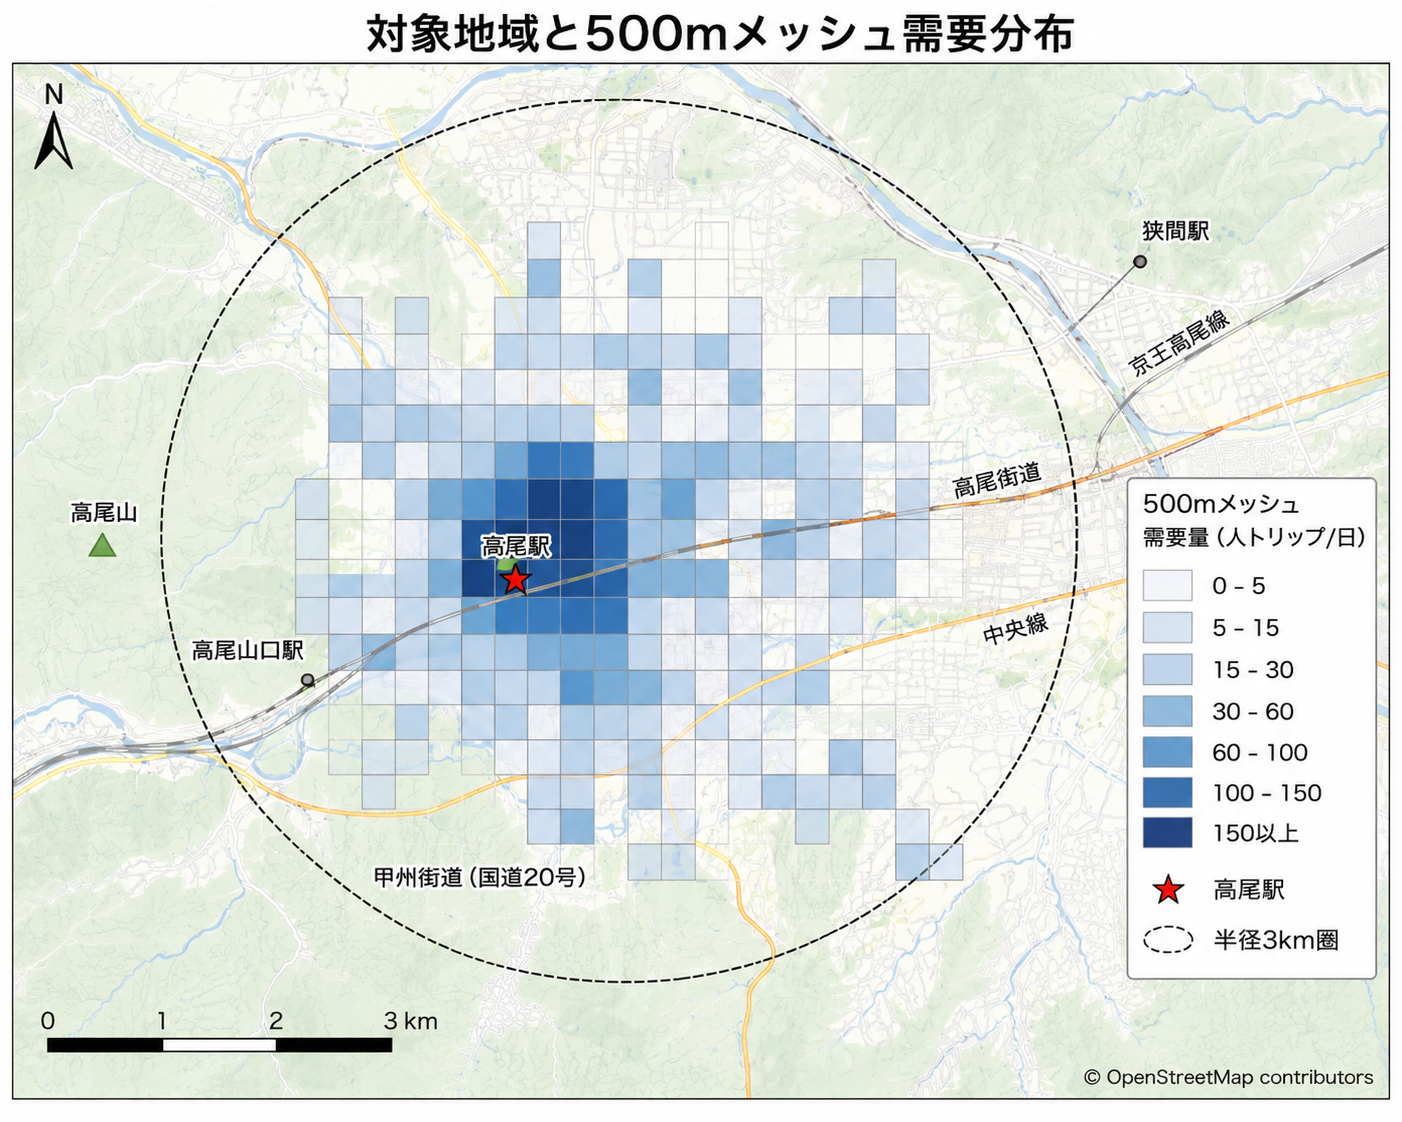
\includegraphics[width=\linewidth]{assets/optimization/optimization/column/fig_mesh_demand.png}
   \captionof{figure}{対象地域と500mメッシュ需要分布}
   \label{fig:takao_mesh}
 \end{center}

*公平性指標は、各個人の支援必要度をもとにゾーン単位で集計した。

\[
s_i = w_1 E_i + w_2 L_i + w_3 C_i + w_4 D_i + w_5 A_i
\]

\[
fairness\_ratio_z
=
\frac{1}{N_z}
\sum_{i \in z} s_i
\]

ここで、
$E_i$ は高齢者、
$L_i$ は免許非保有、
$C_i$ は自由に使える自動車なし、
$D_i$ は外出困難、
$A_i$ は高齢者同行
を表す0/1変数である。
なお、本分析における fairness\_ratio は厳密な福祉指標ではなく、移動制約のある需要を相対的に重視するための proxy として扱っている。
\paragraph{初期分析：3種類のサービス設計}
まず、設計思想の違いを比較するため、以下の3種類のモデルを比較した。

\begin{itemize}
  \item ① 半径型（radius）：高尾駅から一定距離圏内を一括してサービス対象とする。実装容易性を重視した単純な構造。
  \item ② 分散型（demand-based）：需要の大きいゾーンを個別に選択し、効率性を重視する構造。
  \item ③ カバー率型（coverage）：一定割合以上の需要を必ずカバーし、公平性・公共性を重視する構造。
\end{itemize}

比較の結果、カバー率を高めるほどサービス時間が増加し、効率性と公平性の間に明確なトレードオフが存在することが確認された。
また、需要の大きいゾーンを優先する分散型では効率性が高い一方、空間的な偏りが生じやすいことが示唆された。表\ref{tab:results_comparison}に3種類のサービス設計比較を示す。

% 表を入れる場合
 \begin{center}
   \begin{tabular}{lll}
     \toprule
     モデル & 特徴 & 主な示唆 \\
     \midrule
     半径型 & 実装容易性重視 & シンプルだが公平性が不明確 \\
     分散型 & 効率性重視 & 需要偏在で空間的偏りが生じやすい \\
     カバー率型 & 公共性重視 & coverage 増加で service time が増加 \\
     \bottomrule
   \end{tabular}
   \captionof{table}{最適化結果比較}
   \label{tab:results_comparison}
 \end{center}

\paragraph{モデル化}
今回は、本格的なVRPではなく、複数拠点配置＋需要ゾーン割当問題として定式化した。
各需要ゾーンは、選択された拠点のいずれかに割り当てられる。
高尾駅は必ず使用する拠点とし、追加拠点を候補集合から選択する。

サービス時間は、拠点からゾーンへの往復時間に加えて、乗降・待機バッファおよび高尾駅との接続コストを含む近似値として定義した。

\[
t_{ij}
=
2 \times \frac{l_{ij}}{v} \times 60
+
b
+
\gamma \times \frac{h_j}{v} \times 60
\]

ここで、
$l_{ij}$ は拠点 $j$ からゾーン $i$ までの距離[km]、
$v$ は平均速度[km/h]、
$b$ は乗降・待機バッファ[min]、
$h_j$ は拠点 $j$ と高尾駅との距離[km]、
$\gamma$ は駅接続コストの重みである。

この式は、端末交通として各拠点が高尾駅と接続される必要性を近似的に表現したものである。

解法には0-1整数計画（MILP）を用い、目的関数は総サービス時間の最小化とした。

決定変数は以下のとおりである。

\[
x_j = 
\begin{cases}
1 & \text{拠点 } j \text{ を使用する場合} \\
0 & \text{それ以外}
\end{cases}, \qquad
y_{ij} =
\begin{cases}
1 & \text{ゾーン } i \text{ を拠点 } j \text{ に割り当てる場合} \\
0 & \text{それ以外}
\end{cases}
\]

ここで、
$d_i$ はゾーン $i$ の有効需要（effective demand）、
$t_{ij}$ は拠点 $j$ がゾーン $i$ を担当する場合のサービス時間[min]、
$y_{ij}$ はゾーン $i$ を拠点 $j$ に割り当てるかを表す0/1変数である。
なお、繰り返しになるが、有効需要は各ゾーン需要の20\%と仮定した。
また、
$f_i$ はゾーン $i$ の公平性指標、
$C_j$ は拠点 $j$ の処理可能容量を表す。

目的関数は次の形を想定した。

\[
\min \sum_i \sum_j d_i t_{ij} y_{ij}
\]


制約としては、以下の通り、coverage 制約、fairness 制約、拠点数制約、容量制約、割当制約を設定した。

\begin{align*}
&\sum_i d_i z_i \ge \alpha \sum_i d_i
&& \text{(coverage 制約)} \\
&\sum_i d_i f_i z_i \ge \beta \sum_i d_i f_i
&& \text{(fairness 制約)} \\
&\sum_j x_j = P
&& \text{(拠点数制約)} \\
&\sum_j y_{ij} \le 1
&& \forall i \quad \text{(割当制約)} \\
&y_{ij} \le x_j
&& \forall i,j \\
&\sum_i d_i t_{ij} y_{ij}
\le
C_j x_j
&& \forall j \quad \text{(容量制約)}
\end{align*}

\paragraph{計算条件}
高尾駅は必須拠点とし、追加拠点数 $P$ を変化させる。
coverage threshold は 0.4、0.5、0.6 を比較し、総車両台数 fleet を変更した。
さらに、nearest-$k$ 制約を導入し、$k=1$ に近づくほど各拠点の担当圏域が独立する条件を検討した。

% 表を入れる場合
 \begin{center}
   \begin{tabular}{ll}
     \toprule
     項目 & 内容 \\
     \midrule
     対象地域 & 高尾駅周辺3km圏 \\
     需要単位 & 500mメッシュ \\
     effective demand & demand の20\% \\
　　　fleet & 18 / 24 \\ 
     必拠点 & 高尾駅 \\
     追加拠点数 $P$ & 1-4 \\
     coverage threshold & 0.4, 0.5, 0.6 \\
     fairness\_threshold & 0.3 \\ 
     nearest-$k$ 制約 & $k=1$ に近い条件 \\
     \bottomrule
   \end{tabular}
   \captionof{table}{主要パラメータ一覧}
   \label{tab:parameters}
 \end{center}


\paragraph{計算結果}
最適解の一例として、$P=3$ の場合には「高尾駅 + candidate\_6 + candidate\_8」が選択された。図\ref{fig:optimal_locations}に最適拠点配置結果を示す。
このとき、coverage は約0.5、capacity utilization は約1.0 となり、車両容量制約が強く効いていることが確認された。
図\ref{fig:tradeoff}に示すように，coverage を高めると総サービス時間が大きく増加し、効率性と公共性のトレードオフが確認された。
また、fleet 数を減少させた場合には、coverage 制約を満たす解が存在しない infeasible ケースが確認された。
これは、自動運転オンデマンド交通の成立性が、需要量だけでなく投入可能な車両規模にも強く依存することを示している。
一方で、fleet 数を増加させても、拠点配置や coverage 条件が同一である場合には、総サービス時間の改善は限定的であった。
したがって、fleet 数は「効率性」よりも「サービス成立性」を左右する要因として機能したと考えられる。

% 図を入れる場合
 \begin{center}
   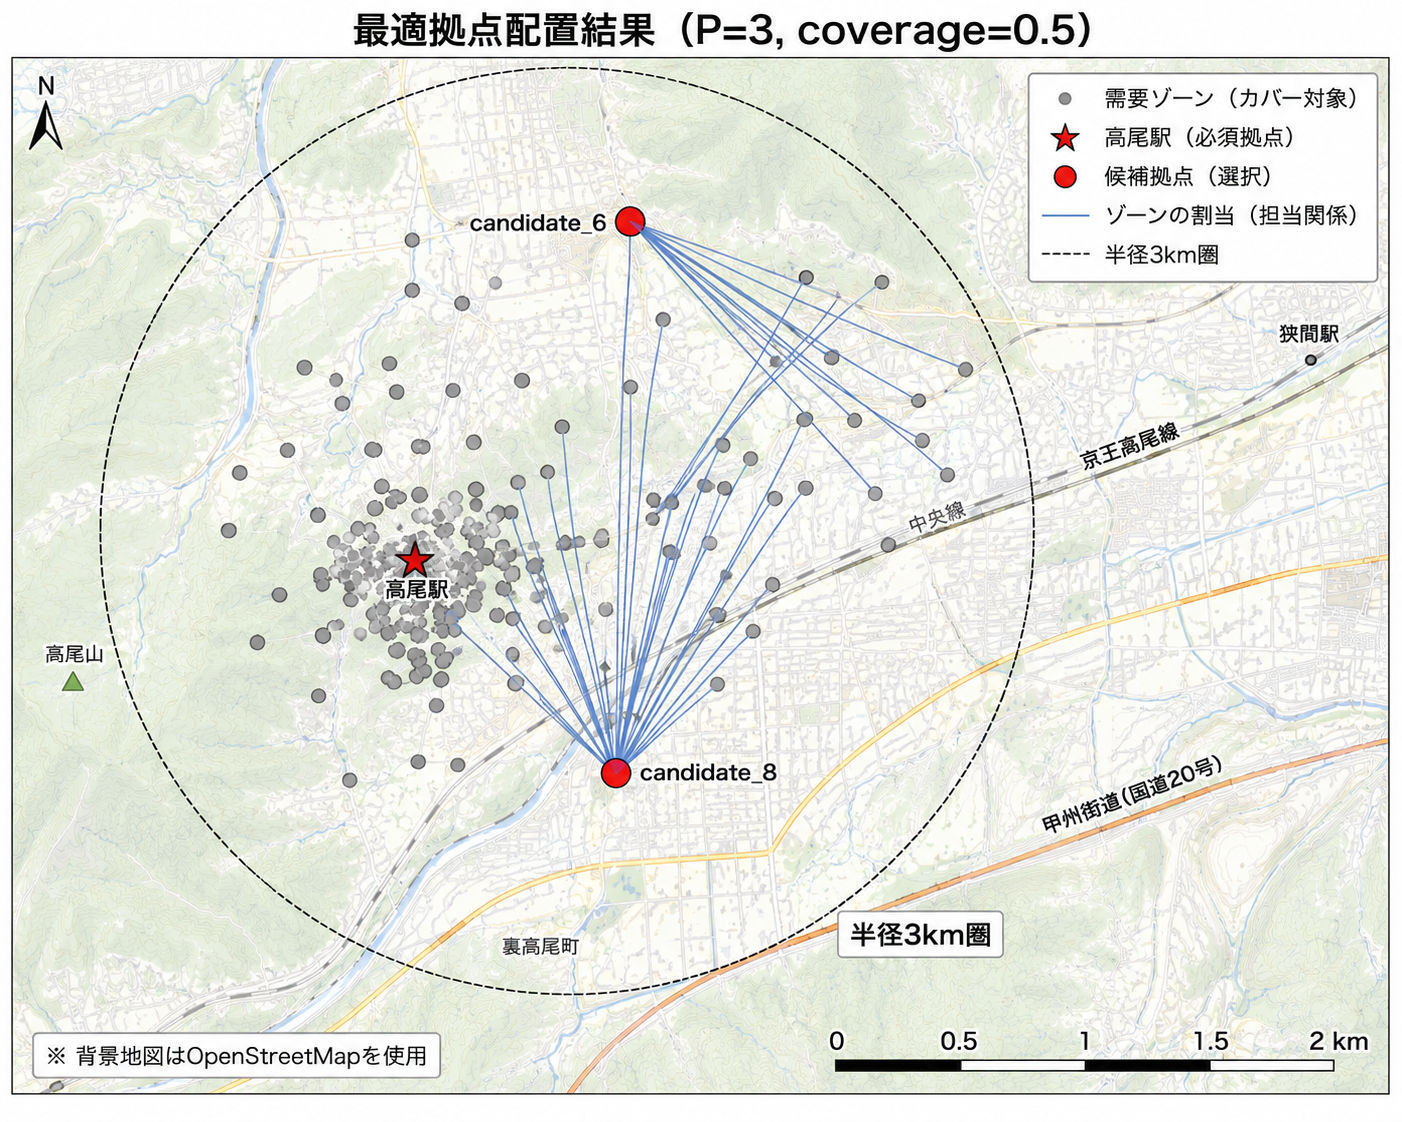
\includegraphics[width=\linewidth]{assets/optimization/optimization/column/fig_optimal_hubs.png}
   \captionof{figure}{最適拠点配置結果}
   \label{fig:optimal_locations}
 \end{center}

% 図を入れる場合
 \begin{center}
   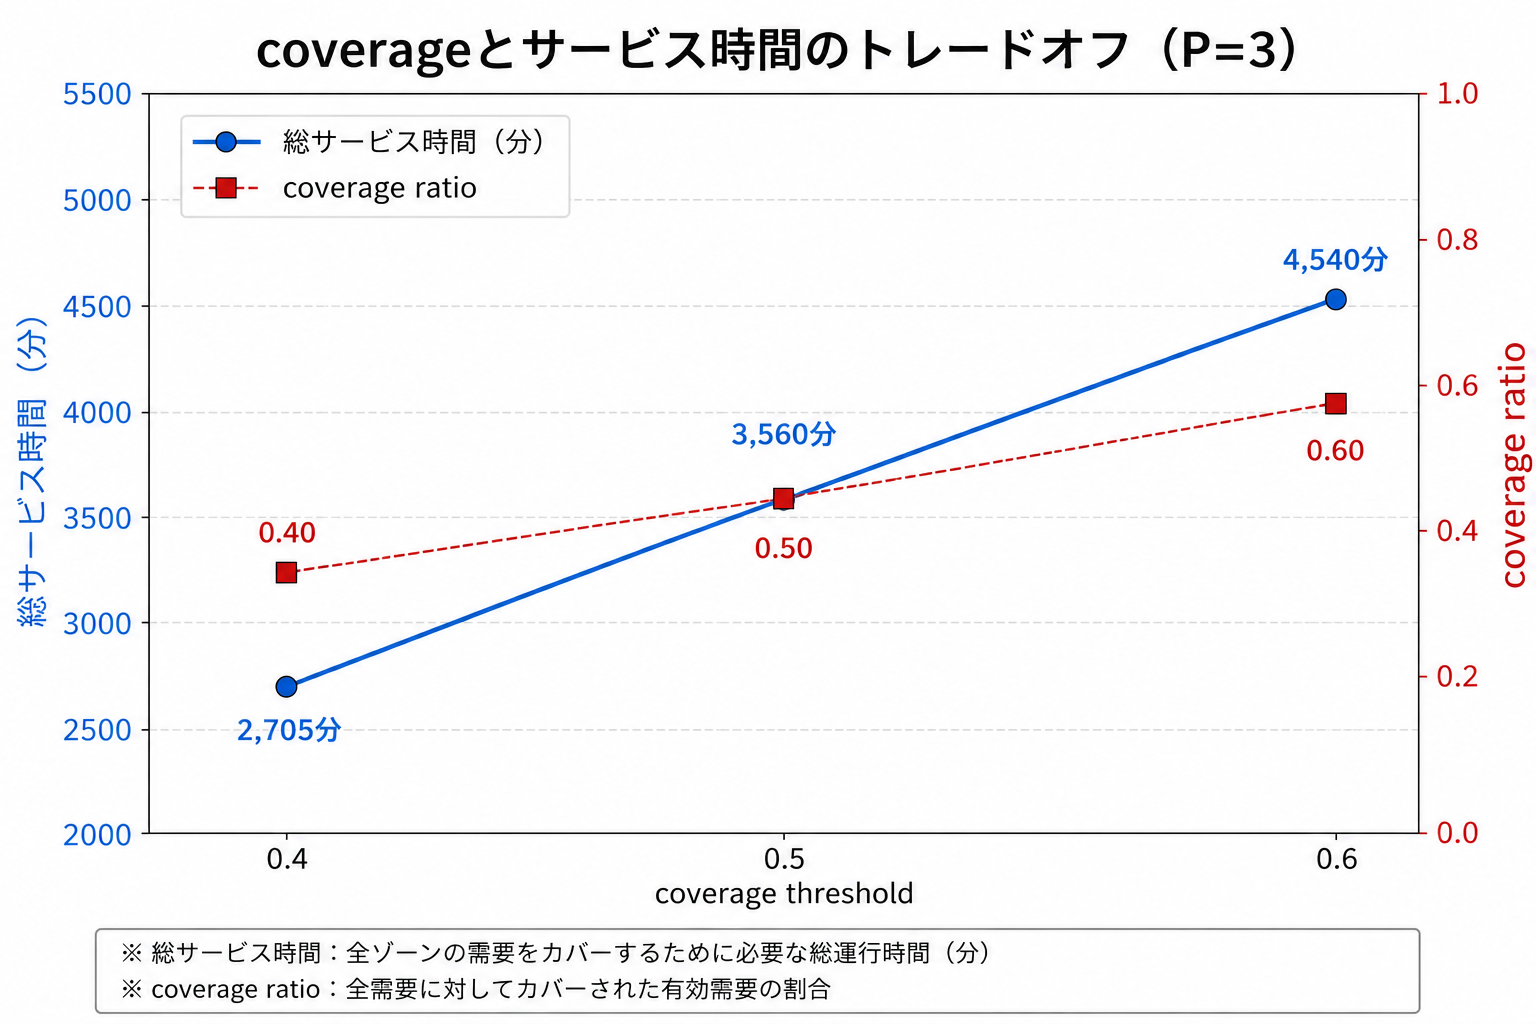
\includegraphics[width=\linewidth]{assets/optimization/optimization/column/fig_tradeoff.png}
   \captionof{figure}{coverage と service time のトレードオフ}
   \label{fig:tradeoff}
 \end{center}

\begin{center}
\begin{tabular}{lrrrrr}
\toprule
ケース & 選択拠点数 & coverage\_ratio & fairness\_coverage\_ratio & total\_service\_time\_min & capacity\_utilization\_mean \\ 
\midrule
P1\_k8 & 1 & 0.5 & 0.526 & 3006.6 & 0.651 \\ 
P2\_k8 & 2 & 0.5 & 0.517 & 3167.1 & 0.651 \\ 
P3\_k8 & 3 & 0.5 & 0.515 & 3633.2 & 0.651 \\ 
P4\_k8 & 4 & 0.5 & 0.511 & 3884.2 & 0.732 \\ 
cov40\_k8 & 3 & 0.4 & 0.4 & 2805.2 & 0.52 \\ 
cov50\_k8 & 3 & 0.5 & 0.515 & 3633.2 & 0.651 \\ 
cov60\_k8 & 3 & 0.6 & 0.618 & 4407.1 & 0.781 \\ 
beta00\_k8 & 3 & 0.5 & 0.515 & 3633.2 & 0.651 \\ 
beta05\_k8 & 3 & 0.5 & 0.515 & 3633.2 & 0.651 \\ 
beta10\_k8 & 3 & 0.5 & 0.515 & 3633.2 & 0.651 \\ 
\bottomrule
\end{tabular}
\captionof{table}{最適化結果比較}
\label{tab:results}
\end{center}

\paragraph{分析と考察}
本分析では、表\ref{tab:results}に示す通り、拠点数 $P$ を増加させても効率性が大きく改善するとは限らず、むしろ coverage の設定や車両容量制約が支配的であることが示された。
一般には拠点数を増やすことで各ゾーンまでの距離が短縮される可能性があるが、本分析では、追加拠点と高尾駅との接続コストや coverage 制約の影響により、総サービス時間が必ずしも減少しなかった。
したがって、単に拠点数を増加させるのではなく、拠点配置と担当圏域を一体的に設計する必要があると考えられる。

都市部では需要密度が高いため、「どこをカバーするか」よりも「限られた車両容量でどれだけ効率的に運用できるか」が主要な制約となる可能性がある。
一方、地方部では需要分布がより分散するため、拠点配置そのものが支配的な問題となることが考えられる。

\paragraph{今後の展望}
本分析を発展させるためには、道路ネットワークを用いた厳密なルーティングや公共施設を考慮した拠点配置、nearest-$k$ 制約の厳密化が求められる。
さらに、地方部への展開や避難・物流との統合的分析も今後の課題である。
\end{column}
\clearpage


%-------------------------------------------------------
%参考文献（末尾に必ず記述）
%-------------------------------------------------------
\addcontentsline{toc}{section}{参考文献}
\bibliographystyle {stone-ship}
\bibliography{../src/bibliography/optimization}

%% ============================================================
%% machine_learning.tex
%%
%% 機械学習関連の章を束ねる親ファイル
%% ============================================================
\chapter{機械学習の基礎}
\chapterauthor{古橋郁一}

%% ============================================================
%% machine_learning.tex
%%
%% 機械学習関連の章を束ねる親ファイル
%% ============================================================
\chapter{機械学習の基礎}
\chapterauthor{古橋郁一}

%% ============================================================
%% machine_learning.tex
%%
%% 機械学習関連の章を束ねる親ファイル
%% ============================================================
\chapter{機械学習の基礎}
\chapterauthor{古橋郁一}

\input{chapters/machine_learning/machine_learning.tex}
\input{chapters/machine_learning/machine_learning_column.tex}
\input{chapters/machine_learning/reinforcement_learning.tex}
\input{chapters/machine_learning/reinforcement_learning_column.tex}
\input{chapters/machine_learning/generative_model.tex}
\input{chapters/machine_learning/generative_model_column.tex}

% ==================================================================
% 参考文献
% ==================================================================
\addcontentsline{toc}{section}{参考文献}
\bibliographystyle{stone-ship}
\bibliography{../src/bibliography/machine_learning}

\clearpage
\begin{column}{コラム}
（内容編集のテスト）
\end{column}
\clearpage
\section{強化学習}

強化学習（reinforcement learning）は，環境との相互作用を通じて意思決定規則を学習し，長期的な累積報酬を最大化するための理論である．教師あり学習では入力と正解の対応が与えられ，教師なし学習では観測データの潜在構造の抽出が中心となるのに対し，強化学習では各時刻の行動に対して正解が即座に与えられるとは限らない．ある行動の評価は，その後に続く状態遷移と報酬列を通じて初めて定まり，その意味で遅延報酬を本質に含んでいる．

本章の目標は，強化学習を単なるアルゴリズムの集合としてではなく，確率的環境のもとで価値関数または方策を学習し，累積報酬を最適化する統一理論として理解することである．標準的な教科書的整理としては \citet{SuttonBarto2018} が広く参照されるが，本章ではそれを踏まえつつ，交通・都市工学の逐次意思決定問題にも接続しやすい形で議論を組み立てる．まず歴史的流れから問題意識を整理し，次にマルコフ決定過程によって標準的定式化を与える．そのうえで，多腕バンディット問題によって探索と活用の本質を切り出し，動的計画法，価値ベース手法，方策勾配法へと進む．最後に，標準的な設定だけでは捉えきれない発展的話題を概観する．

\subsection{強化学習の歴史}

強化学習の歴史を学ぶ必要があるのは，この分野が単に高性能な手法を寄せ集めて成立したのではなく，逐次意思決定に固有の困難に対する応答として発展してきたからである．信号制御，車両経路選択，需要応答交通の運行計画のような問題では，現在の行動が将来の混雑や待ち時間を変化させ，評価は複数時刻にまたがって現れる．したがって，入力と正解の対応をそのまま学べばよい教師あり学習とは異なり，行動の価値を試行錯誤から推定しなければならない．

このとき難しさの中心にあるのが，遅延報酬，探索と活用のトレードオフ，そして方策依存のデータ生成である．第一に，最終的な成果にどの行動が寄与したかを識別する信用割当ての問題が生じる．第二に，より良い行動を見つけるためには未知の選択肢を試す探索が必要だが，探索を増やせば当面の報酬は失われる．第三に，データは受動的に与えられるのではなく，学習者自身の行動によって生成される．これらの特徴が，強化学習に独自の理論を要請する．

歴史的源流は，Bellman による動的計画法と最適制御にある\cite{Bellman1957,Puterman1994}．ここで与えられた基本原理は，長期最適化問題を現在の価値と将来の価値の再帰関係として表すベルマン方程式であった．ただし，この枠組みは環境モデル，すなわち状態遷移確率と報酬関数が既知であることを前提としていた．理論的には明快であっても，未知環境から経験を通じて学ぶという強化学習本来の状況には，そのままでは適用できなかった．

この不足を埋めたのが時間差分学習（temporal-difference learning）である．\citet{Sutton1988}は，将来の完全な帰結を待たず，次時刻の価値推定を足場にして現在の価値を更新するブートストラップの考え方を定式化した．これにより，モンテカルロ法のようにエピソード終了まで待たなくても逐次的に価値を学習できるようになった．ベルマン方程式は，解析のための式であるだけでなく，学習更新式の源泉になったのである．

さらに，\citet{WatkinsDayan1992}による Q 学習は，行動価値関数を直接学ぶことで，環境モデルなしに最適方策へ近づく道を与えた．ここで重要なのは，価値推定と制御の問題が統合されたことである．TD 学習が与えられた方策の価値推定を中心にしていたのに対し，Q 学習は最大演算を通じて最適方策そのものを目指した．

状態空間が高次元化すると，表形式の価値関数では表現能力が不足する．この制約を緩和したのが深層強化学習であり，とくに DQN は画像入力から行動価値を学ぶ代表的成功例となった\cite{Mnih2015}．AlphaGo 以降は，価値学習，方策学習，探索，計画を組み合わせる深層強化学習が急速に発展した\cite{Silver2016}．ただし，この発展は流行紹介として理解するべきではない．本質は，既知モデルから未知モデルへ，表形式から関数近似へ，価値推定から方策最適化へと理論の焦点が拡張された点にある．

同時に，価値ベース手法だけでは連続行動空間や確率的方策の直接最適化に限界があることも明らかになった．\citet{Williams1992}に始まる方策勾配法は，方策を直接最適化対象とする考え方を与え，後に Actor-Critic や PPO のような実用的手法へ発展した\cite{Schulman2015,Schulman2017}．この歴史を貫いているのは，強化学習を「環境との相互作用のもとで累積報酬を最大化する確率的意思決定問題」としてどう定式化し，どう近似的に解くかという問いである．次節では，その標準的枠組みとしてマルコフ決定過程を導入する．

\subsection{マルコフ決定過程}

強化学習を厳密に論じるには，何が状態であり，何が行動であり，何が確率的に変化し，何を最大化したいのかを明示する必要がある．そのための標準的枠組みがマルコフ決定過程（Markov decision process; MDP）である．MDP によって，遅延報酬，価値関数，方策最適化という本章の主要概念を一つの数理的言語で記述できる．

\paragraph*{定義}
MDP は，状態空間 $\mathcal{S}$，行動空間 $\mathcal{A}$，遷移確率 $P(s' \mid s,a)$，報酬関数 $r(s,a,s')$，割引率 $\gamma$ からなる組
\begin{equation}
(\mathcal{S}, \mathcal{A}, P, r, \gamma)
\end{equation}
として与えられる．ここで $s \in \mathcal{S}$ は現在状態，$a \in \mathcal{A}$ は現在行動，$s' \in \mathcal{S}$ は次状態を表す．遷移確率 $P(s' \mid s,a)$ は，状態 $s$ で行動 $a$ を選んだときに次状態が $s'$ になる条件付き確率であり，報酬関数 $r(s,a,s')$ はその遷移に対応する即時報酬の期待値である．割引率 $\gamma \in [0,1)$ は，将来報酬をどの程度現在価値として重視するかを表す係数である．

時刻 $t$ に状態 $s_t$ を観測し，行動 $a_t$ を選び，報酬 $r_t$ を受け取って次状態 $s_{t+1}$ へ移るとする．このとき，時刻 $t$ 以降の累積割引報酬，すなわちリターン $G_t$ を
\begin{equation}
G_t = \sum_{k=0}^{\infty} \gamma^k r_{t+k}
\end{equation}
と定義する．添字 $k$ は現在から何ステップ先の報酬かを表し，$\gamma^k$ はその報酬に掛かる割引である．有限ホライズンではこの和は終端時刻までの有限和となり，無限ホライズンでは $\gamma < 1$ によって収束が保証される．

MDP の核心はマルコフ性にある．これは，次状態と次報酬の条件付き分布が，過去全体ではなく現在状態と現在行動だけで決まるという仮定であり，
\begin{equation}
\mathbb{P}(s_{t+1},r_t \mid s_0,a_0,\ldots,s_t,a_t)
=
\mathbb{P}(s_{t+1},r_t \mid s_t,a_t)
\end{equation}
と書ける．この仮定が重要なのは，現在状態が将来予測に必要な情報を十分に要約しているとみなせるからである．その結果，長期最適化問題を再帰式として記述できる．

\paragraph*{定義}
方策（policy）$\pi(a \mid s)$ は，状態 $s$ のもとで行動 $a$ を選ぶ条件付き確率である．決定論的方策では各状態に一つの行動が対応し，確率的方策では複数の行動に確率が割り当てられる．方策 $\pi$ が与えられたとき，状態価値関数（state-value function）$V^\pi(s)$ と行動価値関数（action-value function）$Q^\pi(s,a)$ を
\begin{align}
V^\pi(s) &= \mathbb{E}_\pi[G_t \mid s_t=s], \\
Q^\pi(s,a) &= \mathbb{E}_\pi[G_t \mid s_t=s, a_t=a]
\end{align}
と定義する．$\mathbb{E}_\pi[\cdot]$ は，方策 $\pi$ と遷移確率 $P$ のもとでの期待値である．$V^\pi(s)$ は状態 $s$ にいることの長期的な良さを，$Q^\pi(s,a)$ は状態 $s$ で行動 $a$ を取ることの長期的な良さを表す．

これらの価値関数は，ベルマン期待方程式を満たす．状態価値関数については
\begin{align}
V^\pi(s)
&=
\sum_{a \in \mathcal{A}} \pi(a \mid s)
\sum_{s' \in \mathcal{S}} P(s' \mid s,a)
\left[
r(s,a,s') + \gamma V^\pi(s')
\right]
\end{align}
が成り立つ．同様に，行動価値関数は
\begin{align}
Q^\pi(s,a)
&=
\sum_{s' \in \mathcal{S}} P(s' \mid s,a)
\left[
r(s,a,s') + \gamma \sum_{a' \in \mathcal{A}} \pi(a' \mid s') Q^\pi(s',a')
\right]
\end{align}
を満たす．ここで $a' \in \mathcal{A}$ は次状態 $s'$ における次の行動である．価値が即時報酬と将来価値の和として再帰的に分解されることが，強化学習の理論的出発点である．

最適方策 $\pi^\ast$ は，全状態で価値を最大化する方策として定義される．対応する最適状態価値関数 $V^\ast(s)$ と最適行動価値関数 $Q^\ast(s,a)$ は
\begin{align}
V^\ast(s) &= \max_\pi V^\pi(s), \\
Q^\ast(s,a) &= \max_\pi Q^\pi(s,a)
\end{align}
であり，ベルマン最適方程式
\begin{align}
V^\ast(s)
&=
\max_{a \in \mathcal{A}}
\sum_{s' \in \mathcal{S}} P(s' \mid s,a)
\left[
r(s,a,s') + \gamma V^\ast(s')
\right], \\
Q^\ast(s,a)
&=
\sum_{s' \in \mathcal{S}} P(s' \mid s,a)
\left[
r(s,a,s') + \gamma \max_{a' \in \mathcal{A}} Q^\ast(s',a')
\right]
\end{align}
を満たす．最大演算は，将来にわたって最も価値の高い行動を選ぶという最適制御の原理を表している．

有限ホライズンと無限ホライズン，エピソード型と継続型の区別も重要である．有限ホライズンでは終端時刻が存在し，無限ホライズンでは割引率が重要になる．エピソード型では終端状態に達すると課題が終了するのに対し，継続型ではタスクが終わらないため，交通流制御のような問題では長期的安定性をどう定義するかが論点になる．次節では，状態遷移という複雑さを一度外し，探索と活用の本質だけを切り出した多腕バンディット問題を考える．

\subsection{多腕バンディット問題}\label{subsec:bandit}

MDP は強化学習の標準形であるが，状態遷移まで含めると探索と活用の本質が見えにくくなることがある．そこで，多腕バンディット問題（multi-armed bandit problem）を導入する．これは状態遷移を持たず，未知の行動価値を試行錯誤によって学ぶという構造だけを残した問題であり，強化学習の基礎概念を理解するうえで有用である\cite{Auer2002,LattimoreSzepesvari2020}．

\paragraph*{定義}
$K$ 本の腕を持つバンディットを考える．各腕 $i \in \{1,\ldots,K\}$ を選ぶと，未知分布に従う報酬が得られ，その期待値を $\mu_i$ とする．時刻 $t$ に選ばれる腕を $A_t$，得られる報酬を $r_t$ と書く．この問題には状態遷移がなく，意思決定は「次にどの腕を引くか」だけである．最適腕の期待報酬を $\mu^\ast=\max_i \mu_i$ とすると，目標は時刻 $T$ までの累積期待報酬を最大化することである．

このとき，性能評価には後悔（regret）がよく用いられる．累積後悔 $R_T$ を
\begin{equation}
R_T
=
T \mu^\ast - \mathbb{E}\left[\sum_{t=1}^{T} r_t\right]
\end{equation}
と定義すると，これは「常に最適腕だけを引いた場合に比べてどれだけ損をしたか」を表す．強化学習全体では累積報酬最大化が中心目的であるが，バンディットでは後悔最小化の形で理論解析が明確になる．

最も単純な戦略の一つが $\epsilon$-greedy である．これは確率 $1-\epsilon$ で現在までに推定された最良の腕を選び，確率 $\epsilon$ で一様ランダムに探索する方法である．ここで $\epsilon \in [0,1]$ は探索率を表す．直感的には，既知の有望な腕を主に活用しつつ，未知の腕をときどき試すことで誤った早期収束を防ぐ．ただし，不確実性の大きさを腕ごとに使い分けないため，探索の効率は高くない．

これに対して，上側信頼限界法（upper confidence bound; UCB）は，推定平均と不確かさの両方を用いる\cite{Auer2002}．腕 $i$ の時刻 $t-1$ までの経験平均を $\hat{\mu}_i(t-1)$，その腕を選んだ回数を $N_i(t-1)$ とすると，典型的には
\begin{equation}
A_t
=
\mathop{\mathrm{arg\,max}}_i
\left[
\hat{\mu}_i(t-1)
+
c \sqrt{\frac{\log t}{N_i(t-1)}}
\right]
\end{equation}
で腕を選ぶ．ここで $c>0$ は探索の強さを調整する定数である．右辺第二項は未観測性に対応し，試行回数が少ない腕ほど大きくなる．したがって UCB は，「現在よさそうな腕」だけでなく「まだ十分試していないので本当は良いかもしれない腕」も積極的に選ぶ．

もう一つの代表的方法が Thompson sampling である\cite{Thompson1933}．これは，各腕の平均報酬に関する事後分布を持ち，そこから仮想的な平均報酬 $\tilde{\mu}_i$ をサンプルして
\begin{equation}
A_t = \mathop{\mathrm{arg\,max}}_i \tilde{\mu}_i
\end{equation}
とする方法である．たとえばベルヌーイ報酬では，成功確率にベータ分布を置くことで計算が容易になる．Thompson sampling の特徴は，探索が外的なランダム化としてではなく，パラメータ不確実性のベイズ的表現から自然に導かれる点にある．

バンディット問題が MDP より簡単なのは，状態遷移がないため，長期的な信用割当てを考える必要がないからである．一方で，本質的に共通している点も明確である．すなわち，未知の環境で累積報酬を最大化するには，不確実性のもとで探索と活用を両立させなければならない．この意味で，多腕バンディットは強化学習の縮約版である．次節では，再び状態遷移を導入し，ただし環境モデルが既知である場合の計画法として動的計画法を扱う．

\subsection{動的計画法}

動的計画法（dynamic programming）が必要になるのは，環境モデルが既知であれば，経験から学ぶ前に理論上の最適解を計算できるからである．これは現実にはしばしば非現実的な仮定であるが，強化学習アルゴリズムの基準点としてきわめて重要である．モデル未知の場合の TD 学習や Q 学習は，多くの場合この枠組みをサンプル近似したものと理解できる．

\paragraph*{定義}
方策 $\pi$ に対するベルマン作用素 $T^\pi$ を
\begin{equation}
(T^\pi V)(s)
=
\sum_{a \in \mathcal{A}} \pi(a \mid s)
\sum_{s' \in \mathcal{S}} P(s' \mid s,a)
\left[
r(s,a,s') + \gamma V(s')
\right]
\end{equation}
と定義する．ここで $V$ は任意の状態価値関数である．同様に，最適ベルマン作用素 $T_\ast$ を
\begin{equation}
(T_\ast V)(s)
=
\max_{a \in \mathcal{A}}
\sum_{s' \in \mathcal{S}} P(s' \mid s,a)
\left[
r(s,a,s') + \gamma V(s')
\right]
\end{equation}
と定義する．ベルマン期待方程式は $V^\pi = T^\pi V^\pi$，ベルマン最適方程式は $V^\ast = T_\ast V^\ast$ という不動点方程式になる．

\paragraph*{アルゴリズム}
方策評価（policy evaluation）は，固定された方策 $\pi$ の価値関数 $V^\pi$ を求める手続きである．初期関数 $V_0$ を任意に取り，
\begin{equation}
V_{k+1} = T^\pi V_k
\end{equation}
と反復すると，$V_k$ は $V^\pi$ に近づく．直感的には，価値は終端報酬や高報酬状態から逆向きに伝播する．まず 1 ステップ先の価値が更新され，その情報がさらに前の状態へ波及していくのである．

方策改善（policy improvement）は，現在の価値関数にもとづいてより良い行動を選ぶ段階である．すなわち，各状態 $s$ について
\begin{equation}
\pi'(s)
\in
\mathop{\mathrm{arg\,max}}_{a \in \mathcal{A}}
\sum_{s' \in \mathcal{S}} P(s' \mid s,a)
\left[
r(s,a,s') + \gamma V^\pi(s')
\right]
\end{equation}
とすれば，新しい方策 $\pi'$ は少なくとも $\pi$ と同程度，通常はそれ以上の価値を持つ．これは，現在の価値評価に照らして各状態で最善の 1 ステップ行動を選べば，方策全体が改善することを意味している．

方策反復（policy iteration）は，方策評価と方策改善を交互に行う方法である．
\begin{enumerate}
\item 現在の方策 $\pi_k$ を評価して $V^{\pi_k}$ を求める．
\item $V^{\pi_k}$ に対して貪欲化を行い，新しい方策 $\pi_{k+1}$ を得る．
\item 方策が変化しなくなるまで反復する．
\end{enumerate}

価値反復（value iteration）は，方策評価を完全に解かずに最適ベルマン作用素を直接適用する方法であり，
\begin{equation}
V_{k+1} = T_\ast V_k
\end{equation}
を反復する．その後，各状態で価値を最大化する行動を選べば最適方策が得られる．価値反復は「いま分かっている将来価値に照らして最善の 1 ステップ選択」を毎回価値へ織り込む方法であり，計画と改善が一体化されている．

\paragraph*{定理}
ベルマン作用素が収束をもたらす理由は，割引率 $\gamma < 1$ のもとで縮小写像になるからである．最大ノルム $\|V-W\|_\infty = \max_{s \in \mathcal{S}} |V(s)-W(s)|$ を用いると，
\begin{align}
\|T^\pi V - T^\pi W\|_\infty &\le \gamma \|V-W\|_\infty, \\
\|T_\ast V - T_\ast W\|_\infty &\le \gamma \|V-W\|_\infty
\end{align}
が成り立つ．誤差が反復ごとに少なくとも $\gamma$ 倍に縮むため，不動点に向かって収束する．直感的には，遠い将来の影響が割引によって弱まり，誤差が増幅しないことを意味する．

動的計画法は理論上の理想解法である一方，遷移確率と報酬関数が既知でなければ使えない．そのため，モデル未知の状況では期待値計算を実際の観測遷移で置き換える必要がある．次節では，その橋渡しとして TD 学習から Q 学習へ至る価値ベース手法を扱う．

\subsection{価値ベース手法：Q学習, Deep-Q学習}

現実の強化学習では，環境モデルが未知であることが多い．したがって，動的計画法のように遷移確率の期待値を厳密に計算することはできず，経験から価値を学習しなければならない．価値ベース手法は，価値関数を学ぶことを通じて最適方策を間接的に得る方法であり，モデル未知環境における強化学習の中心的流儀である．

出発点となるのは TD 学習である．状態価値関数 $V$ に対する TD(0) の更新は
\begin{equation}
V(s_t)
\leftarrow
V(s_t) + \alpha
\left[
r_t + \gamma V(s_{t+1}) - V(s_t)
\right]
\end{equation}
で与えられる．ここで $\alpha \in (0,1]$ は学習率である．角括弧内の量
\begin{equation}
\delta_t = r_t + \gamma V(s_{t+1}) - V(s_t)
\end{equation}
を TD 誤差という．$\delta_t$ は，現在の価値予測が 1 ステップ先の観測を踏まえてどれだけ過小または過大であったかを示す量であり，価値修正の方向と大きさを与える信号である．

制御問題では，状態そのものの価値だけでなく，各行動の価値を知る必要がある．そこで行動価値関数 $Q(s,a)$ を学習する．Q 学習は
\begin{equation}
Q(s_t,a_t) \leftarrow Q(s_t,a_t) + \alpha \left[r_t + \gamma \max_{a'} Q(s_{t+1},a') - Q(s_t,a_t)\right]
\end{equation}
という更新式で定義される\cite{WatkinsDayan1992}．ここで $a' \in \mathcal{A}$ は次状態 $s_{t+1}$ における候補行動であり，$\max_{a'} Q(s_{t+1},a')$ は将来に最善行動を選ぶと仮定した価値である．この最大演算を通じて，Q 学習は最適方策へ向かう．

Q 学習の重要な特徴は off-policy 学習である点にある．すなわち，実際にデータを収集する行動方策と，更新式の内部で想定している目標方策が一致していなくてもよい．たとえば $\epsilon$-greedy によって探索を行いながら，更新時には貪欲方策を想定できる．これに対し SARSA は
\begin{equation}
Q(s_t,a_t)
\leftarrow
Q(s_t,a_t) + \alpha
\left[
r_t + \gamma Q(s_{t+1},a_{t+1}) - Q(s_t,a_t)
\right]
\end{equation}
と，実際に選ばれた次行動 $a_{t+1}$ を用いて更新する on-policy 手法である．Q 学習が将来の最良行動に基づく強気の更新であるのに対し，SARSA は探索を含んだ現在の方策をそのまま評価する．

表形式の Q 学習は，状態空間と行動空間が小さいときには有効であるが，高次元状態では破綻する．画像入力や多数の交通状態特徴量のような状況では，各 $(s,a)$ に対して表を持つことができない．このとき必要になるのが関数近似であり，Deep Q-Network（DQN）はニューラルネットワーク $Q(s,a;\theta)$ によって行動価値関数を近似する\cite{Mnih2015}．

DQN では，TD ターゲットを
\begin{equation}
y_t = r_t + \gamma \max_{a'} Q(s_{t+1},a';\theta^-)
\end{equation}
と置き，損失関数
\begin{equation}
L_t(\theta)
=
\left[
y_t - Q(s_t,a_t;\theta)
\right]^2
\end{equation}
を最小化する．ここで $\theta$ は学習中のネットワークの重み，$\theta^-$ はターゲットネットワークの重みである．もし右辺のターゲットまで同じ重みで毎回更新すると，目標そのものが激しく動くため学習が不安定化する．ターゲットネットワークはこの問題を緩和し，更新先を一時的に固定する役割を果たす．

もう一つの重要要素が経験再生（experience replay）である．これは，過去の遷移 $(s_t,a_t,r_t,s_{t+1})$ をバッファに蓄積し，そこから無作為にミニバッチを抽出して学習する仕組みである．経験再生が必要なのは，連続する遷移が強く相関しているため，そのまま学習すると勾配推定が不安定になるからである．無作為抽出により相関を弱められ，同じ経験を複数回再利用できるのでデータ効率も向上する．DQN の安定化は，この経験再生とターゲットネットワークに大きく依存している．

その後，Double DQN は最大演算に由来する過大評価を軽減し，dueling network は状態価値とアドバンテージを分離して表現することで学習効率を高めた．しかし中心的な論点は，TD 学習の再帰構造を深層関数近似とどう両立させるかにある．価値ベース手法の長所は，離散行動空間では各行動の価値を直接比較できること，ベルマン方程式との結びつきが明瞭であることである．一方で，連続行動空間では $\max_{a'} Q(s_{t+1},a')$ の計算が難しく，確率的方策の直接制御や制約付き最適化にも不向きである．この限界が，次節で扱う方策勾配法の必要性を生む．

\subsection{方策勾配法：Actor-Critic, PPO}

価値ベース手法の限界が明確になるのは，連続行動空間や確率的方策の直接最適化を考えるときである．ロボット制御のように行動が実数ベクトルで表される場合，離散行動に対する最大化は自然ではない．また，探索を方策の分布そのものに埋め込みたい場合には，価値関数を介した間接的な最適化より，方策を直接最適化する方が適切である．この問題意識から方策勾配法が導入される．

パラメータ $\theta$ を持つ方策を $\pi_\theta(a \mid s)$ とし，期待リターンを
\begin{equation}
J(\theta) = \mathbb{E}_{\pi_\theta}[G_0]
\end{equation}
と定義する．ここで $\mathbb{E}_{\pi_\theta}[\cdot]$ は，方策 $\pi_\theta$ と環境ダイナミクスに従って生成される軌道に関する期待値である．方策勾配法の目標は，$J(\theta)$ を最大化するように $\theta$ を更新することである．

\paragraph*{定理}
方策勾配の基本形は
\begin{equation}
\nabla_\theta J(\theta) = \mathbb{E}\left[\nabla_\theta \log \pi_\theta(a_t|s_t)\, G_t\right]
\end{equation}
で与えられる\cite{Williams1992}．ここで $\nabla_\theta$ はパラメータ $\theta$ に関する勾配，$\log \pi_\theta(a_t \mid s_t)$ は選択された行動の対数確率，$G_t$ は時刻 $t$ 以降のリターンである．この式は，良い帰結をもたらした行動の確率を高め，悪い帰結をもたらした行動の確率を下げるという学習規則を正当化する．

REINFORCE はこの勾配を標本平均で近似する最も基本的なアルゴリズムであり，
\begin{equation}
\theta \leftarrow \theta + \alpha \sum_t \nabla_\theta \log \pi_\theta(a_t \mid s_t) G_t
\end{equation}
と更新する．ここで $\alpha$ は学習率である．REINFORCE は不偏推定量を与えるが，$G_t$ の分散が大きく，学習が不安定になりやすい．とくにホライズンが長い問題では，分散の削減が不可欠になる．

そこでベースライン $b(s_t)$ を導入し，
\begin{equation}
\nabla_\theta J(\theta)
=
\mathbb{E}\left[
\nabla_\theta \log \pi_\theta(a_t \mid s_t)
\left(G_t - b(s_t)\right)
\right]
\end{equation}
と書き換える．$b(s_t)$ が状態のみに依存する限り，勾配の期待値は変わらず，分散だけを減らせる．とくに $b(s_t)=V^\pi(s_t)$ と置くと，アドバンテージ関数
\begin{equation}
A^\pi(s_t,a_t) = Q^\pi(s_t,a_t) - V^\pi(s_t)
\end{equation}
が現れる．これは，状態 $s_t$ において行動 $a_t$ が平均的行動よりどれだけ良かったかを表す量である．

Actor-Critic はこの考え方を実装する枠組みである．Actor は方策 $\pi_\theta(a \mid s)$ を表し，Critic は価値関数，典型的には $V(s;w)$ を推定する．ここで $w$ は Critic のパラメータである．Critic は TD 学習により
\begin{equation}
\delta_t = r_t + \gamma V(s_{t+1};w) - V(s_t;w)
\end{equation}
を計算する．この TD 誤差 $\delta_t$ は，1 ステップのアドバンテージ推定として機能する．したがって Actor は
\begin{equation}
\theta \leftarrow \theta + \alpha \, \delta_t \, \nabla_\theta \log \pi_\theta(a_t \mid s_t)
\end{equation}
と更新できる．$\delta_t$ が正なら行動確率を増やし，負なら減らすので，Critic の価値推定が Actor の改善方向を与えることになる．

実際の深層強化学習では，方策更新が大きすぎると性能が急激に悪化することがある．TRPO は新旧方策の距離に制約を課すことでこの問題に対処したが\cite{Schulman2015}，計算は比較的重い．これに対し PPO は，同じ問題意識をより簡潔な目的関数で扱う\cite{Schulman2017}．

PPO では，古い方策を $\pi_{\theta_{\mathrm{old}}}$，新しい方策を $\pi_\theta$ とし，確率比
\begin{equation}
r_t(\theta)
=
\frac{\pi_\theta(a_t \mid s_t)}{\pi_{\theta_{\mathrm{old}}}(a_t \mid s_t)}
\end{equation}
を考える．さらに $A_t$ を推定アドバンテージとすると，clip された目的関数は
\begin{equation}
L^{\mathrm{clip}}(\theta)
=
\mathbb{E}
\left[
\min\left(
r_t(\theta)A_t,\,
\mathrm{clip}\left(r_t(\theta),1-\epsilon,1+\epsilon\right)A_t
\right)
\right]
\end{equation}
と書かれる．ここで $\epsilon > 0$ は更新幅を制御するハイパーパラメータであり，$\mathrm{clip}(\cdot)$ は値を区間 $[1-\epsilon,1+\epsilon]$ に切り詰める演算である．新方策が旧方策から過度に離れると，利得の増加が頭打ちになるため，大きすぎる更新が抑制される．

PPO が実用上の標準手法とみなされるのは，信頼領域の思想を保ちつつ，実装が容易でミニバッチ最適化とも相性がよいからである．とくに連続行動空間，大規模関数近似，確率的方策の直接制御が必要な問題では，方策勾配法の重要性は大きい．価値ベース手法が価値推定を通じて行動を導くのに対し，方策勾配法は望ましい行動分布そのものを直接整形する．この違いが，現代の深層強化学習における両者の役割分担を定めている．

\subsection{発展的話題}

標準的な MDP，価値学習，方策勾配法は強力な枠組みであるが，現実世界の課題をそのまま捉えられるわけではない．実応用では，環境モデルは未知であり，観測は不完全であり，安全制約があり，データ収集が高価であることが多い．この節では，そのような制約のもとで基本理論がどのように拡張されるかを概観する．

\subsubsection{モデルベース強化学習}

モデルベース強化学習（model-based RL）が必要になるのは，サンプル効率を高めたいからである．モデルフリー手法は柔軟であるが，多数の試行を要する．実機ロボットや都市交通制御では，試行そのものが高価であり，環境モデルを全く使わない学習は非現実的であることが多い．

基本的な発想は，遷移モデル $\hat{P}$ と報酬モデル $\hat{r}$ をデータから学習し，その近似モデルの内部で計画やロールアウトを行うことである．モデルが十分正確なら，実環境での試行を減らしつつ方策改善ができる．一方で，モデル誤差は長期予測で蓄積しやすいため，短い計画区間に限定する，モデル不確実性を推定する，モデルフリー更新と併用するといった工夫が必要になる．

\subsubsection{オフライン強化学習}

オフライン強化学習（offline RL）が必要になるのは，新たな探索を現場で行えない状況があるからである．医療，金融，公共交通運用のような領域では，学習のために試しに危険な行動を取ることは許されない．そのため，過去に収集された固定データ集合
\begin{equation}
\mathcal{D} = \{(s,a,r,s')\}
\end{equation}
だけを用いて方策を学習する．

ここでの難しさは，データに含まれていない行動を価値関数が過大評価しやすい点にある．すなわち，分布外の行動に対する楽観主義が性能劣化を招く．このため，オフライン強化学習では，行動方策に近い範囲で保守的に学習する，価値推定を意図的に低めに補正する，行動分布そのものを制約する，といった工夫が中心課題となる．

\subsubsection{部分観測 MDP}

標準的 MDP では現在状態が将来予測に必要な情報を十分含むと仮定したが，現実には状態そのものが直接観測できないことが多い．部分観測 MDP（partially observable MDP; POMDP）は，この状況を扱うための拡張であり，エージェントは状態 $s_t$ の代わりに観測 $o_t$ だけを得る．

このとき単一の観測だけでは意思決定に必要な情報が不足することがある．たとえば需要の潜在状態や他主体の意図は直接見えない．そこで，過去観測から信念状態を更新して隠れ状態の分布を内部状態として扱う方法や，再帰型ネットワークによって観測履歴を潜在表現へ圧縮する方法が用いられる．POMDP は，マルコフ性を放棄するのではなく，観測から実質的なマルコフ表現を再構成する問題として理解できる．

\subsubsection{探索の高度化}

疎な報酬や長いホライズンを持つ問題では，単純な $\epsilon$-greedy では有益な経験に到達しにくい．このため，探索そのものを主題化する必要がある．代表的な考え方の一つが内発的動機づけ（intrinsic motivation）であり，新規性や予測誤差にもとづく探索ボーナスを外的報酬に加える．

たとえば修正報酬を
\begin{equation}
r_t' = r_t + \beta b_t
\end{equation}
と書けば，$\beta > 0$ は探索ボーナスの重み，$b_t$ は新規性や予測困難性を表す量である．ほかにも，不確実性の大きい行動を積極的に高く見る楽観主義や，事後分布から方策をサンプルする posterior sampling がある．探索は単なるランダム化ではなく，情報獲得をどう最適化するかという設計問題へ発展している．

\subsubsection{多エージェント強化学習}

多エージェント強化学習（multi-agent RL; MARL）が必要になるのは，環境が単一主体ではなく複数主体の相互作用で構成されるからである．交通流や配車市場では，各主体が学習することで他主体にとっての環境も変化する．その結果，各エージェントから見れば環境は非定常となり，単一エージェント MDP の仮定がそのままでは通用しにくい．

ここでの問題は，協調と競争をどう扱うかである．協調型では局所情報から全体効率を高める共同方策を構成する必要があり，競争型では相手の学習を見越した戦略的適応が求められる．実用的には，学習時には全体情報を利用し，実行時には各主体が局所観測だけで動く centralized training with decentralized execution が広く用いられる．

\subsubsection{模倣学習と逆強化学習}

現実の問題では，報酬関数を適切に設計すること自体が難しい．自動運転や運行制御では，「安全」「快適」「効率」といった複数の目的を単一の数値報酬に落とし込むのが容易ではない．このとき，人間や既存システムの行動データを利用する方法として，模倣学習（imitation learning）と逆強化学習（inverse RL）が重要になる．

模倣学習は専門家の行動系列から直接方策を学ぶ方法であり，探索コストを大きく削減できる．逆強化学習は，専門家行動の背後にある報酬関数を推定し，その推定報酬のもとで方策最適化を行う方法である．前者が「どう行動するか」を学ぶのに対し，後者は「何を目的としているか」を推定する．いずれも，標準的な MDP＋価値学習＋方策勾配だけでは扱いにくい現実的制約を補う拡張である．

\subsection{まとめ}

本章では，強化学習を環境との相互作用のもとで長期的な意思決定を最適化する理論として体系的に整理した．まず，教師あり学習や教師なし学習では十分に捉えられない遅延報酬，試行錯誤，探索と活用の問題から強化学習が必要になることを述べ，その歴史が動的計画法，TD 学習，Q 学習，深層関数近似，方策勾配法へと展開してきた流れを確認した．

続いて，マルコフ決定過程によって状態，行動，遷移確率，報酬，割引率，方策，価値関数を定義し，ベルマン方程式が強化学習全体の再帰的骨格であることを示した．多腕バンディット問題は，探索と活用の本質を状態遷移なしに抽出する縮約版として位置づけられ，動的計画法は環境モデル既知の場合の理論的基準点を与えた．そのうえで，モデル未知の状況では TD 学習と Q 学習が経験から価値を推定し，DQN が高次元状態へ拡張した．さらに，価値ベース手法の限界を受けて，方策勾配法，Actor-Critic，PPO が方策そのものを直接最適化する枠組みを与えることを見た．最後に，モデルベース強化学習，オフライン強化学習，POMDP，探索の高度化，多エージェント強化学習，模倣学習と逆強化学習を通じて，現実世界では未知性，部分観測，安全制約，データ収集制約が基本理論の拡張を要請することを確認した．以上を通じて，強化学習は「環境との相互作用のもとで価値関数または方策を学習し，長期的な意思決定を最適化する理論」として理解されるべきである．

\clearpage
\begin{column}{探索と活用のジレンマ（多腕バンディット問題の実験） - 長田晴人}

\ \textbf{実験設定と評価指標}\\
強化学習の重要なテーマの一つに，\textbf{探索と活用のジレンマ}がある．
ここでは，第\ssref{subsec:bandit}小節で取り上げた多腕バンディット問題を用いて，
いくつかの探索手法を同一条件で比較し，パラメータの違いが学習曲線に
どのように現れるかを確認する．

\ バンディット問題の名前は，スロットマシンが ``one-armed bandit''
と呼ばれていたことに由来する．
レバーを引くと確率的に報酬が得られるが，どのレバーの期待報酬が高いかは
プレイヤーには分からない．
本実験では，6本の腕 $a\in\{1,\ldots,6\}$ を持つバンディットを考え，
各腕を選ぶと確率
\[
    p=\left(\frac{1}{20},\frac{1}{10},\frac{1}{10},\frac{1}{10},\frac{1}{2},\frac{3}{4}\right)
\]
で報酬 $1$ が得られ，それ以外では報酬 $0$ が得られるとする．
学習者はこの真の確率を知らず，実際に得られた報酬から各腕の行動価値を推定する．
この問題では第6腕が最適腕であるが，第5腕も比較的高い報酬確率を持つため，
初期の偶然によって第5腕を過大評価し，第6腕を十分に試さないまま学習が進む可能性がある．

\ 比較する手法は，$\varepsilon$-greedy，softmax，UCB，optimistic 初期値，
Thompson sampling である．
このコラムの目的は，平均報酬と累積後悔の推移を通じて，
\textbf{探索の強さ}や\textbf{価値推定の方法}が学習過程に与える影響を観察することである．
確率的なばらつきを抑えるため，各条件について1000回の独立試行を行い，
その平均を学習曲線としてプロットする．

\ まず，行動価値の更新方法と腕の選択方法を分けて整理する．
表\ref{tab:bandit-value-update}は「得られた報酬をどのように価値推定へ反映するか」を表し，
表\ref{tab:bandit-action-selection}は「推定された価値にもとづいて次にどの腕を選ぶか」を表す．

\begin{center}
    \small
    \renewcommand{\arraystretch}{1.55}
    \captionof{table}{行動価値の更新方法}
    \label{tab:bandit-value-update}
    \begin{tabular}{p{0.42\linewidth}p{0.50\linewidth}}
      \toprule
      手法・式 & 備考 \\
      \midrule

      \textbf{標本平均手法}
      \[
      Q_t(a)
      =
      \frac{1}{N_t(a)}
      \sum_{\tau \leq t: A_\tau=a} r_\tau
      \]
      &
      $N_t(a)$ は，時刻 $t$ までに腕 $a$ を選んだ回数である．
      過去に腕 $a$ から得た報酬の平均をそのまま行動価値とする．
      定常環境では自然な推定方法であるが，過去の観測をすべて同じ重みで扱うため，
      非定常環境では古い情報を引きずりやすい．
      \\

      \midrule

      \textbf{逐次的な標本平均}
      \[
      Q_{t+1}(a)
      =
      Q_t(a)
      +
      \frac{1}{N_t(a)}
      \{r_t-Q_t(a)\}
      \]
      &
      標本平均手法を逐次更新の形で書いたものである．
      新しい報酬 $r_t$ と現在の推定値 $Q_t(a)$ の差を，
      選択回数の逆数だけ反映する．
      選択回数が増えるほど，新しい観測の影響は小さくなる．
      \\

      \midrule

      \textbf{固定学習率手法}
      \[
      Q_{t+1}(a)
      =
      Q_t(a)
      +
      \alpha\{r_t-Q_t(a)\}
      \]
      &
      $\alpha \in (0,1]$ は学習率である．
      新しい報酬を一定の重みで反映する方法であり，
      $\alpha$ が大きいほど最近の観測を重視し，小さいほど推定は安定する．
      標本平均手法と異なり，古い観測の影響が相対的に小さくなるため，
      非定常環境に追従しやすい．
      \\

      \bottomrule
    \end{tabular}
\end{center}

\begin{center}
    \small
    \renewcommand{\arraystretch}{1.55}
    \captionof{table}{多腕バンディット問題における腕の選択方法}
    \label{tab:bandit-action-selection}
    \begin{tabular}{p{0.42\linewidth}p{0.50\linewidth}}
      \toprule
      手法・式 & 備考 \\
      \midrule

      \textbf{greedy}
      \[
      A_t
      =
      \arg\max_{a\in\mathcal{A}} Q_t(a)
      \]
      &
      常に現在の推定価値 $Q_t(a)$ が最大の腕を選ぶ．
      探索を行わないため，初期の偶然によって悪い腕を過大評価すると，
      その腕を選び続ける可能性がある．
      \\

      \midrule

      \textbf{$\varepsilon$-greedy}
      \[
      A_t =
      \begin{cases}
      \arg\max\limits_{a\in\mathcal{A}} Q_t(a),
      & \text{確率 } 1-\varepsilon,\\
      \text{ランダムな腕},
      & \text{確率 } \varepsilon
      \end{cases}
      \]
      &
      $\varepsilon \in [0,1]$ は探索率である．
      確率 $\varepsilon$ でランダム探索を行う．
      $\varepsilon$ が大きいほど未知の腕を試しやすいが，
      学習後も低報酬の腕を選ぶ確率が残る．
      $\varepsilon=0$ では greedy と一致する．
      \\

      \midrule

      \textbf{softmax}
      \[
      \Pr(A_t=a)
      =
      \frac{\exp(Q_t(a)/\tau)}
      {\sum_{b\in\mathcal{A}}\exp(Q_t(b)/\tau)}
      \]
      &
      $\tau>0$ は温度パラメータである．
      $\tau$ が大きいほど選択確率は一様に近づき，
      $\tau$ が小さいほど greedy に近づく．
      価値差をどの程度鋭く選択確率に反映するかを決めるスケールパラメータとして解釈できる．
      \\

      \midrule

      \textbf{UCB}
      \[
      A_t
      =
      \arg\max_{a\in\mathcal{A}}
      \left\{
      Q_t(a)
      +
      c\sqrt{\frac{\log t}{N_t(a)}}
      \right\}
      \]
      &
      $c>0$ は探索ボーナスの強さ，
      $N_t(a)$ は腕 $a$ の選択回数である．
      選択回数が少ない腕ほど第2項が大きくなるため，
      未探索の腕を体系的に試す．
      $c$ が大きいほど探索的になり，小さいほど現在の推定価値を重視する．
      \\

      \midrule

      \textbf{optimistic 初期値}
      \[
      Q_0(a)=Q_{\mathrm{init}}
      \qquad
      (Q_{\mathrm{init}}\text{ を大きく設定})
      \]
      &
      $Q_{\mathrm{init}}$ は初期行動価値である．
      行動選択規則そのものではなく，初期価値を高く置くことで探索を促す方法である．
      まだ試していない腕が楽観的に評価されるため，
      明示的なランダム探索を入れなくても複数の腕を試しやすい．
      \\

      \midrule

      \textbf{Thompson sampling}
      \[
      \tilde{\theta}_a \sim P_t(\theta_a),
      \qquad
      A_t=\arg\max_{a\in\mathcal{A}}\mu(a;\tilde{\theta}_a)
      \]
      &
      $P_t(\theta_a)$ は，腕 $a$ の報酬分布のパラメータ $\theta_a$ に関する事後分布である．
      各腕の事後分布からパラメータをサンプリングし，
      そのもとでの期待報酬 $\mu(a;\tilde{\theta}_a)$ が最大の腕を選ぶ．
      今回は Bernoulli 報酬なので，成功確率 $p_a$ の事後分布として
      ベータ分布 $\mathrm{Beta}(\alpha_a,\beta_a)$ を用いる．
      \\

      \bottomrule
    \end{tabular}
\end{center}

\ 累積後悔についても簡単に述べておく．
平均報酬が「どれだけ報酬を得られたか」を表すのに対し，
累積後悔は「最初から最適腕を知っていた場合に比べて，
どれだけ報酬を取り逃したか」を表す．
時刻 $t$ に選んだ腕を $A_t$，その真の報酬確率を $p_{A_t}$，
最適腕の報酬確率を $p^\ast=3/4$ とすると，時刻 $T$ までの累積後悔は
\[
    R_T=\sum_{t=1}^{T}\left(p^\ast-p_{A_t}\right)
\]
で定義される．
この指標を見ることで，探索のために低確率の腕を引いたコストや，
第5腕のような「そこそこ良い腕」に固定されたことによる損失を評価できる．

\begin{center}
  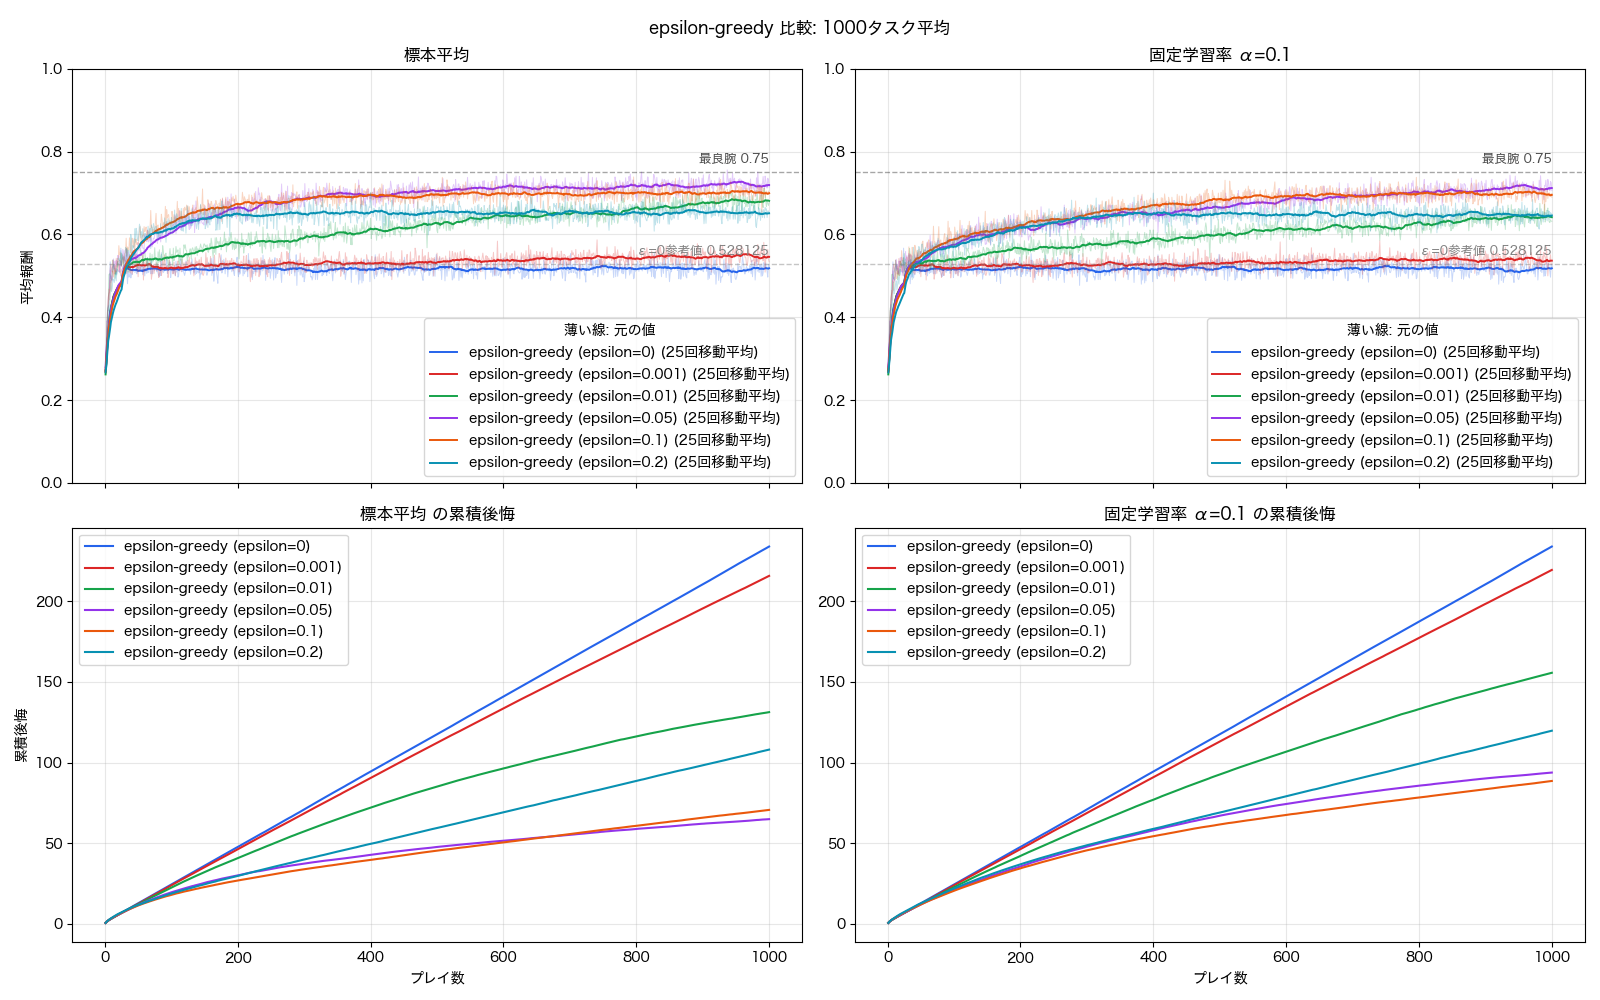
\includegraphics[width=\linewidth]{assets/reinforcement_column/greedy_graph.png}
  \captionof{figure}{greedy 法と $\varepsilon$-greedy 法の学習曲線}
  \label{fig:epsilon-greedy}
\end{center}

\ \textbf{greedy 法と $\varepsilon$-greedy 法}\\
図\ref{fig:epsilon-greedy}では，greedy 法と $\varepsilon$-greedy 法を比較した．
greedy 法は
\[
    A_t=\arg\max_{a\in\mathcal{A}}Q_t(a)
\]
により，常に現在の推定価値が最大の腕を選ぶ方法である．
一方，$\varepsilon$-greedy 法では，確率 $1-\varepsilon$ で greedy な腕を選び，
確率 $\varepsilon$ でランダムに腕を選ぶ．

\ $\varepsilon=0$ の greedy 法では，初期値をすべて $Q_0(a)=0$ とすると，
最初に報酬 $1$ を出した腕に固定されやすい．
報酬が出るまでは同点の腕をランダムに選ぶため，最初に成功する腕が $a$ である確率は
\[
    q_a=\frac{p_a}{\sum_{b=1}^{6}p_b}
\]
と近似できる．
したがって，長期的な平均報酬は
\[
    \bar{r}_{\infty}
    =
    \sum_{a=1}^{6}q_a p_a
    =
    \frac{\sum_{a=1}^{6}p_a^2}{\sum_{a=1}^{6}p_a}
\]
となる．
今回の設定では
\[
    \sum_{a=1}^{6}p_a=\frac{8}{5},
    \qquad
    \sum_{a=1}^{6}p_a^2=\frac{169}{200}
\]
であるから，
\[
    \bar{r}_{\infty}
    =
    \frac{169/200}{8/5}
    =
    \frac{169}{320}
    =
    0.528125
\]
となる．
これは図中の $\varepsilon=0$ の収束値とよく一致している．

\ 一方，$\varepsilon=0.2$ の場合，学習が十分進んで greedy 部分では第6腕を選べるようになったとしても，
全体の $20\%$ はランダムに腕を選ぶ．
このとき長期的な平均報酬はおよそ
\[
    (1-\varepsilon)p^\ast
    +
    \varepsilon \frac{1}{6}\sum_{a=1}^{6}p_a
\]
で与えられる．
今回の設定では $p^\ast=3/4$，
\[
    \frac{1}{6}\sum_{a=1}^{6}p_a
    =
    \frac{4}{15}
\]
であるから，
\[
    (1-0.2)\cdot\frac{3}{4}
    +
    0.2\cdot\frac{4}{15}
    \simeq
    0.653
\]
となる．
図で $\varepsilon=0.2$ の平均報酬が最適腕の $0.75$ より低い値に落ち着くのは，
学習後も一定確率で低報酬の腕を選び続けるためである．
つまり，\textbf{$\varepsilon$ は小さすぎても大きすぎてもよくない}．
今回の結果では，$\varepsilon=0.05$ から $0.1$ 程度が，
初期探索と後半の活用のバランスがよかった．

\ 累積後悔のグラフは，この違いを別の形で示している．
累積後悔の傾きは，各時刻でどれだけ報酬を取り逃しているか，すなわち瞬間的な後悔の大きさを表す．
たとえば，greedy 法が平均報酬 $\bar{r}_{\infty}$ の腕選択に固定されているとき，
累積後悔の傾きはおよそ
\[
    p^\ast-\bar{r}_{\infty}
\]
となる．
$\varepsilon=0$ では
\[
    \frac{3}{4}-0.528125=0.221875
\]
となり，後悔が大きな傾きで増え続ける．
これは，学習が速いというより，早い段階で誤った腕に固定されてしまっている状態である．

\ これに対して，$\varepsilon>0$ では初期に探索を行うため，序盤の累積後悔は増えやすい．
しかし，その探索によって最適腕を発見できれば，その後の累積後悔の傾きは小さくなる．
また，累積後悔の傾きが時間とともに小さく変化し続けている場合には，
腕の選択がまだ改善しており，学習が継続していると解釈できる．
逆に，累積後悔がほぼ直線になった場合には，腕の選択傾向がほぼ固定され，
その時点の方策で一定の損失を出し続けていると考えられる．
これは，初期に損をしてでも正しい腕を見つける「学習の速さ」と，
学習後に不要な探索をどれだけ減らせるかという「最終的な正確性」のトレードオフを表している．

\begin{center}
  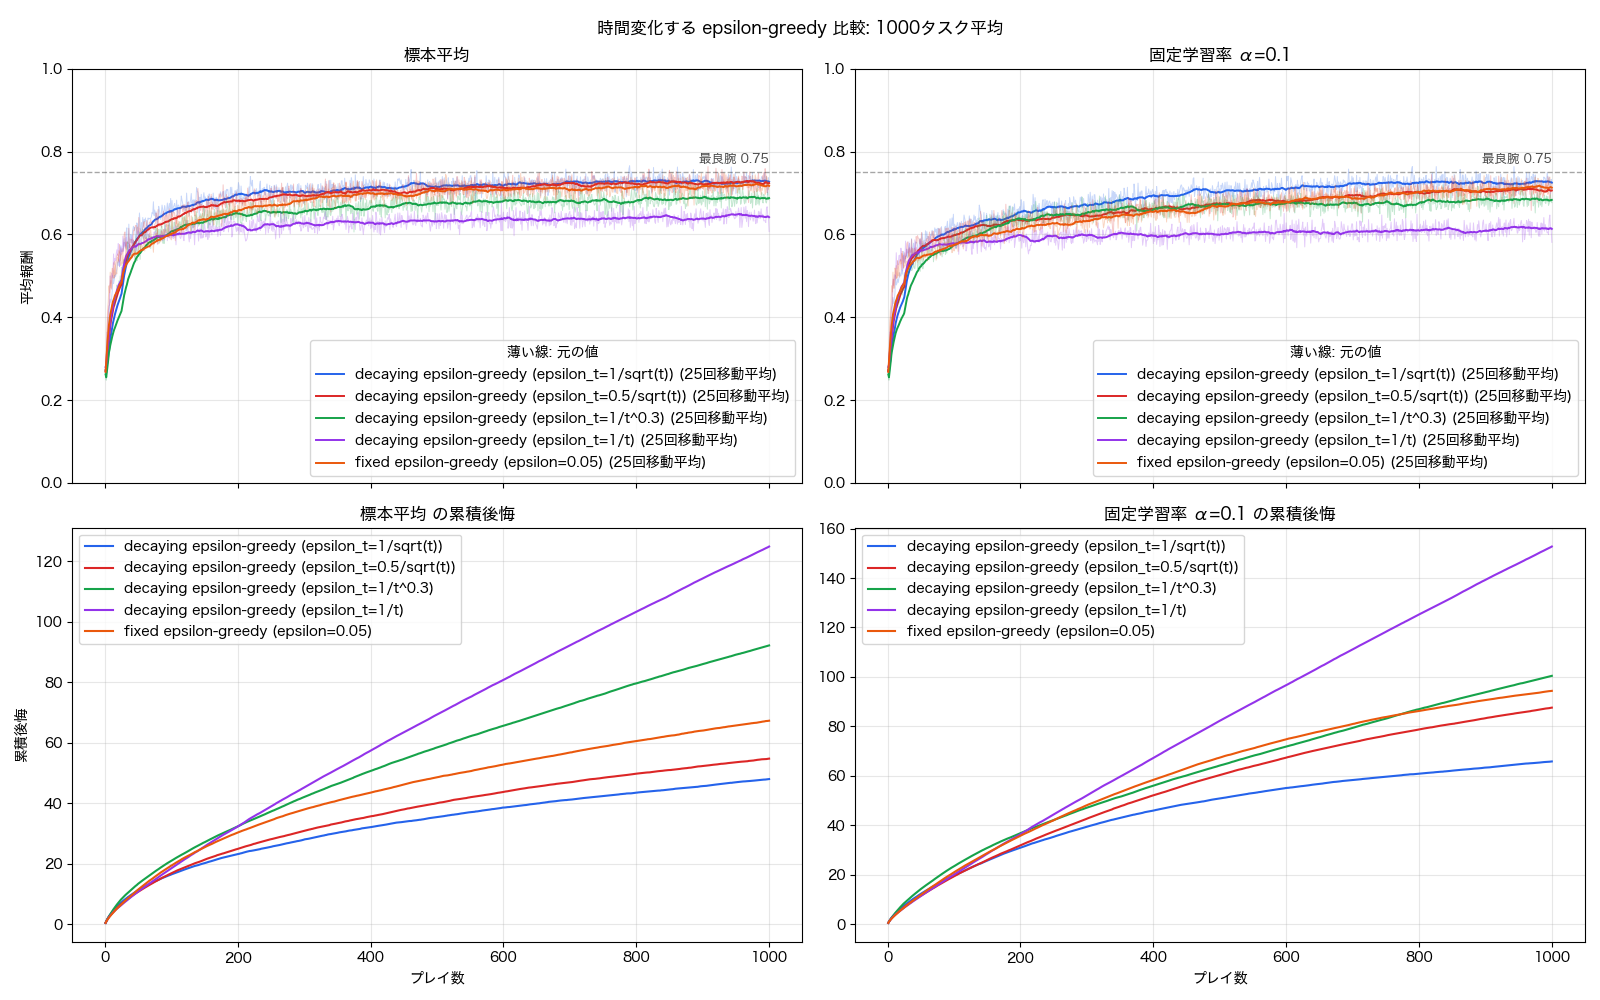
\includegraphics[width=\linewidth]{assets/reinforcement_column/time_greedy.png}
  \captionof{figure}{$\varepsilon$が時間変化する場合の学習曲線}
  \label{fig:decaying-epsilon-greedy}
\end{center}

\ \textbf{時間変化する $\varepsilon_t$-greedy 法}\\
固定した $\varepsilon$ を用いる $\varepsilon$-greedy 法では，
$\varepsilon$ が小さすぎると探索が不足し，初期に高く評価された腕に固定されやすい．
一方で，$\varepsilon$ が大きすぎると，最適腕を見つけた後もランダム探索が残り，
低報酬の腕を選ぶ損失が続いてしまう．
そこで，学習初期には十分に探索し，学習後半では不要な探索を減らすために，
時間とともに探索率を小さくする $\varepsilon_t$-greedy 法を考える．

\ $\varepsilon_t$-greedy 法では，
\[
    A_t =
    \begin{cases}
    \displaystyle \arg\max_{a\in\mathcal{A}} Q_t(a), & \text{確率 } 1-\varepsilon_t,\\
    \text{ランダムな腕}, & \text{確率 } \varepsilon_t
    \end{cases}
\]
として，各時刻 $t$ における探索率 $\varepsilon_t$ を変化させる．
本実験では，
\[
    \varepsilon_t=\frac{1}{\sqrt{t}},\quad
    \varepsilon_t=\frac{0.5}{\sqrt{t}},\quad
    \varepsilon_t=\frac{1}{t^{0.3}},\quad
    \varepsilon_t=\frac{1}{t}
\]
を比較し，固定値 $\varepsilon=0.05$ の場合とも比べた．

\ 図\ref{fig:decaying-epsilon-greedy}を見ると，
$\varepsilon_t=1/\sqrt{t}$ は，平均報酬と累積後悔の両方で比較的良い挙動を示している．
これは，時刻 $T$ までに発生するランダム探索の期待回数から説明できる．
$\varepsilon_t$-greedy 法では，各時刻に確率 $\varepsilon_t$ で探索を行うため，
探索回数 $M_T$ の期待値は
\[
    \mathbb{E}[M_T]
    =
    \sum_{t=1}^{T}\varepsilon_t
\]
である．
腕の本数を $K=6$ とすると，ランダム探索だけで各腕が試される回数の目安は
\[
    \frac{1}{K}\sum_{t=1}^{T}\varepsilon_t
\]
となる．

\ $\varepsilon_t=1/t$ の場合，
\[
    \sum_{t=1}^{T}\frac{1}{t}
    \simeq
    \log T
\]
である．
今回の実験では $T=1000$ なので，$\log 1000 \simeq 6.9$ となり，
各腕をランダム探索で試す回数は平均して1回程度にすぎない．
そのため，早い段階で探索率が小さくなりすぎ，
第6腕を十分に試す前に別の腕へ固定されやすい．

\ 一方，$\varepsilon_t=1/\sqrt{t}$ の場合，
\[
    \sum_{t=1}^{T}\frac{1}{\sqrt{t}}
    \simeq
    2\sqrt{T}
\]
である．
$T=1000$ では $2\sqrt{1000}\simeq 63$ となるため，
各腕はランダム探索だけでも平均して10回程度試される．
今回の報酬確率では，第6腕の報酬確率 $p_6=3/4$ と第5腕の報酬確率 $p_5=1/2$ の差が
\[
    \Delta=p_6-p_5=\frac{1}{4}
\]
と比較的大きい．
そのため，各腕を十数回程度試せば，第6腕が有望であることを発見するきっかけを得やすい．
さらに，$\varepsilon_t=1/\sqrt{t}$ は時間とともに $0$ に近づくため，
最適腕を見つけた後には不要なランダム探索が減り，平均報酬を高く保ちやすい．

\ これに対して，$\varepsilon_t=1/t^{0.3}$ の場合，
\[
    \sum_{t=1}^{T}\frac{1}{t^{0.3}}
    \simeq
    \frac{T^{0.7}}{0.7}
\]
であり，$T=1000$ ではおよそ $180$ 程度になる．
これは $\varepsilon_t=1/\sqrt{t}$ よりも探索回数が多く，
最適腕を発見するうえでは有利である．
しかし，学習後半にもランダム探索が多く残るため，
低報酬の腕を引く損失が続き，累積後悔の増加を抑えにくい．
つまり，$1/t$ は探索が減るのが速すぎ，$1/t^{0.3}$ は探索が残りすぎる．
その中間にある $1/\sqrt{t}$ は，今回の設定では
\textbf{探索不足と探索過多のバランス}がよかったと考えられる．

\ ここで，標本平均と固定学習率の違いにも注目したい．
固定した $\varepsilon$ の実験では両者の差は比較的小さかったが，
時間変化する $\varepsilon_t$ ではその差がより現れている．
標本平均手法では
\[
    Q_{t+1}(a)
    =
    Q_t(a)
    +
    \frac{1}{N_t(a)}\{r_t-Q_t(a)\}
\]
であり，腕 $a$ を多く選ぶほど新しい報酬の重み $1/N_t(a)$ は小さくなる．
一方，固定学習率では
\[
    Q_{t+1}(a)
    =
    Q_t(a)
    +
    \alpha\{r_t-Q_t(a)\}
\]
であり，新しい報酬は常に重み $\alpha$ で反映される．
実際，固定学習率の更新を展開すると
\[
    Q_n
    =
    (1-\alpha)^nQ_0
    +
    \sum_{i=1}^{n}\alpha(1-\alpha)^{n-i}r_i
\]
となり，最近の報酬ほど大きな重みを持つことが分かる．

\ 時間変化する $\varepsilon_t$ では，学習後半の探索機会が減るため，
後から得られた少数の観測をどれだけ強く価値推定に反映できるかが重要になる．
そのため，過去の観測を均等に平均する標本平均よりも，
最近の結果を大きく見る固定学習率の方が，減衰スケジュールの違いに敏感に反応しやすい．
このため，固定 $\varepsilon$ では目立たなかった価値更新方法の違いが，
時間変化する $\varepsilon_t$ の実験ではよりはっきり現れたと考えられる．

\ ただし，この結果は $\varepsilon_t=1/\sqrt{t}$ が一般に最適な減衰率であることを意味しない．
適切な減衰率は，腕の本数，プレイ回数，最適腕と次善腕の報酬確率差，
および価値更新方法に依存する．
今回の6本腕バンディット問題では，$T=1000$ という有限時間の中で，
$1/\sqrt{t}$ が「十分に探索するが，探索し続けすぎない」スケールになっていたと解釈できる．

\begin{center}
  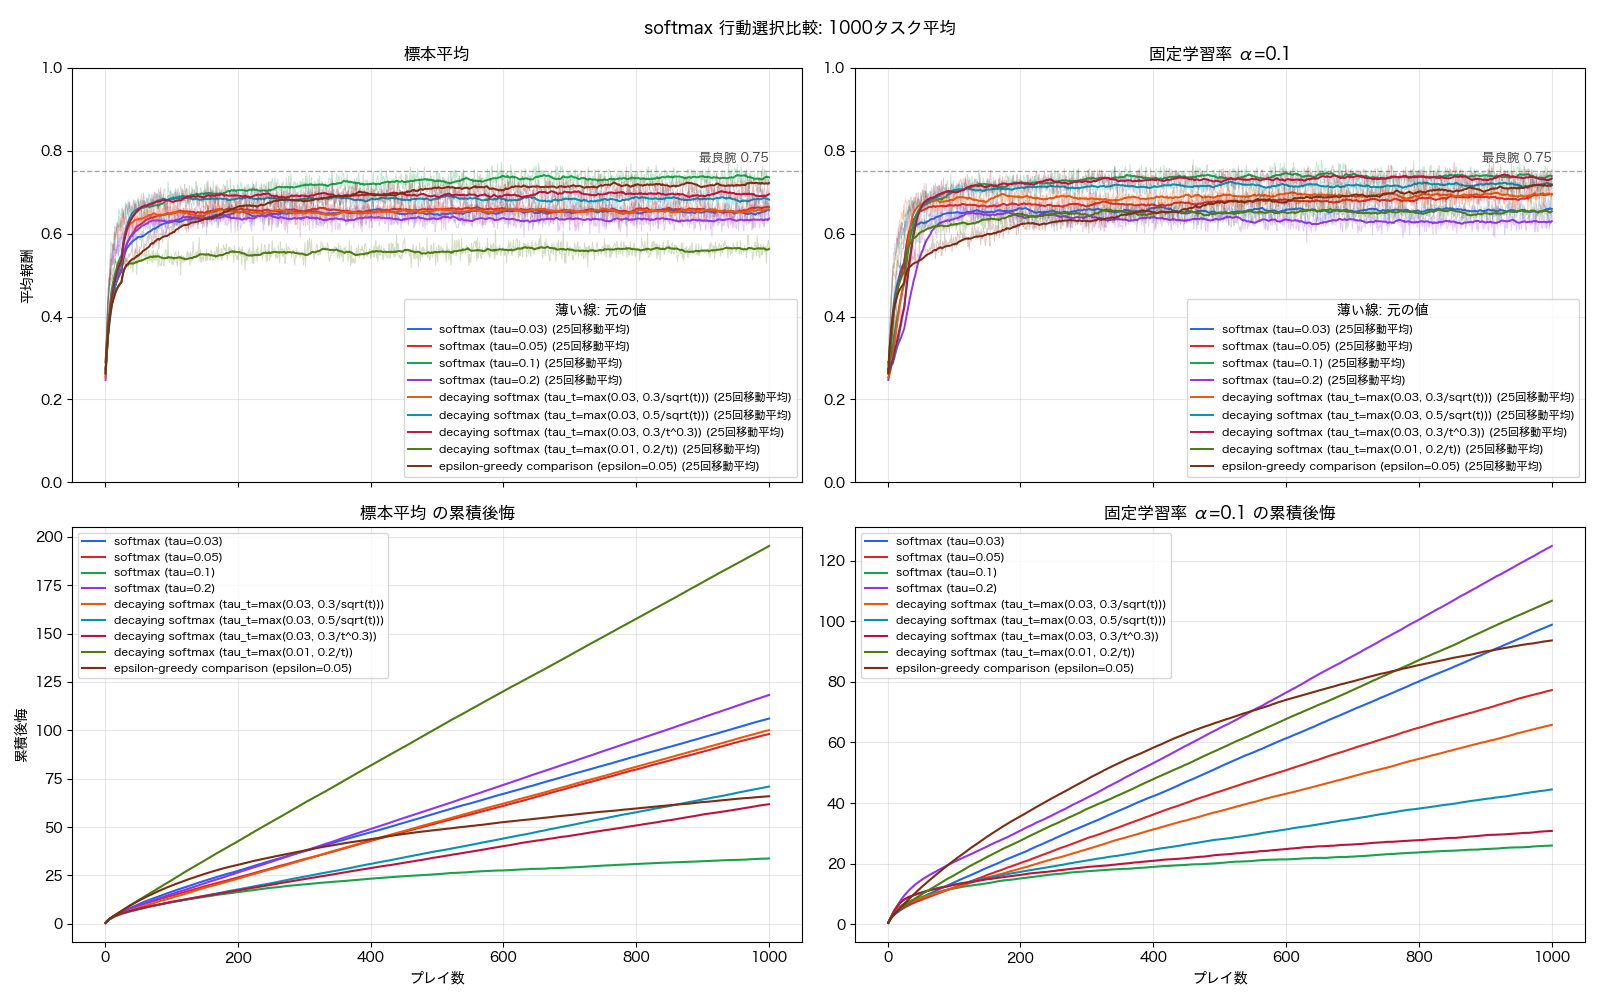
\includegraphics[width=\linewidth]{assets/reinforcement_column/softmax.png}
  \captionof{figure}{softmax 法の学習曲線}
  \label{fig:softmax}
\end{center}

\ \textbf{softmax 法}\\
次に，softmax による行動選択を比較する．
softmax 法では，各腕の推定行動価値 $Q_t(a)$ に対して
\[
    \Pr(A_t=a)
    =
    \frac{\exp(Q_t(a)/\tau)}
    {\sum_{b\in\mathcal{A}}\exp(Q_t(b)/\tau)}
\]
によって選択確率を与える．
ここで $\tau>0$ は温度パラメータであり，
$\tau$ が大きいほど各腕の選択確率は一様に近づき，
$\tau$ が小さいほど greedy 法に近づく．
したがって，$\tau$ は「価値の差をどれくらい鋭く行動選択に反映するか」を決める
スケールパラメータである．

\ 固定温度の結果を見ると，今回の設定では $\tau=0.1$ 付近が比較的よい性能を示している．
この理由は，今回の真の報酬確率の差の大きさから説明できる．
最適腕である第6腕と次善腕である第5腕の報酬確率差は
\[
    p_6-p_5
    =
    \frac{3}{4}-\frac{1}{2}
    =
    \frac{1}{4}
\]
である．
softmax では，2つの腕 $a,b$ の選択確率の比は
\[
    \frac{\Pr(A_t=a)}{\Pr(A_t=b)}
    =
    \exp\left(\frac{Q_t(a)-Q_t(b)}{\tau}\right)
\]
となる．
仮に推定値が真の報酬確率に近づき，
$Q_t(6)-Q_t(5)\simeq 0.25$ であるとすると，
$\tau=0.1$ のとき
\[
    \frac{\Pr(A_t=6)}{\Pr(A_t=5)}
    \simeq
    \exp\left(\frac{0.25}{0.1}\right)
    =
    \exp(2.5)
    \simeq 12.2
\]
となる．
つまり，第6腕は第5腕より十分選ばれやすいが，
第5腕が完全に排除されるほど極端でもない．
この程度の鋭さが，今回の問題では探索と活用のバランスとしてちょうどよかったと考えられる．

\ 一方，$\tau=0.2$ では
\[
    \exp\left(\frac{0.25}{0.2}\right)
    =
    \exp(1.25)
    \simeq 3.5
\]
となり，第6腕と第5腕の選択確率の差がそれほど大きくならない．
そのため，学習後も第5腕や他の腕を選ぶ確率が残りやすく，
平均報酬は最適値 $0.75$ から離れ，累積後悔も増えやすい．
逆に，$\tau=0.03$ のように温度が小さすぎると，
\[
    \exp\left(\frac{0.25}{0.03}\right)
    \simeq
    \exp(8.33)
\]
となり，わずかな価値差でも選択確率が極端に偏る．
学習が十分進んだ後であれば有利に働くが，
初期には $Q_t(a)$ の推定誤差が大きいため，
偶然高く評価された腕に選択が集中しやすい．

\ このように，softmax 法でも\textbf{温度は大きすぎても小さすぎてもよくない}．
今回の6本腕バンディット問題では，最適腕と次善腕の差が $0.25$ であるため，
$\tau=0.1$ 程度にすると
\[
    \frac{p_6-p_5}{\tau}
    =
    \frac{0.25}{0.1}
    =
    2.5
\]
となり，softmax の指数関数によって最適腕を十分に優遇しつつ，
完全な greedy にはならない程度の選択確率が得られる．
これが，固定温度 $\tau=0.1$ が今回うまく働いた主な理由である．

\ さらに，温度を時間とともに変化させる方法も試した．
これは，学習初期には温度を高めにして広く探索し，
学習が進むにつれて温度を下げることで，より価値の高い腕に選択を集中させる方法である．
本実験では，たとえば
\[
    \tau_t=\max\left(0.03,\frac{c}{\sqrt{t}}\right)
\]
のように，温度を減衰させつつ，下限値 $0.03$ を設けた．
下限を置いたのは，温度が小さくなりすぎるとほぼ greedy になり，
わずかな推定誤差にも過剰に反応してしまうためである．
図\ref{fig:softmax}では，温度を適切に減衰させた場合，
固定温度よりも累積後悔の増加を抑えられる場合がある．
これは，序盤では探索によって第6腕を発見する機会を確保し，
後半では温度低下によって第6腕への選択を強められるためである．

\begin{center}
  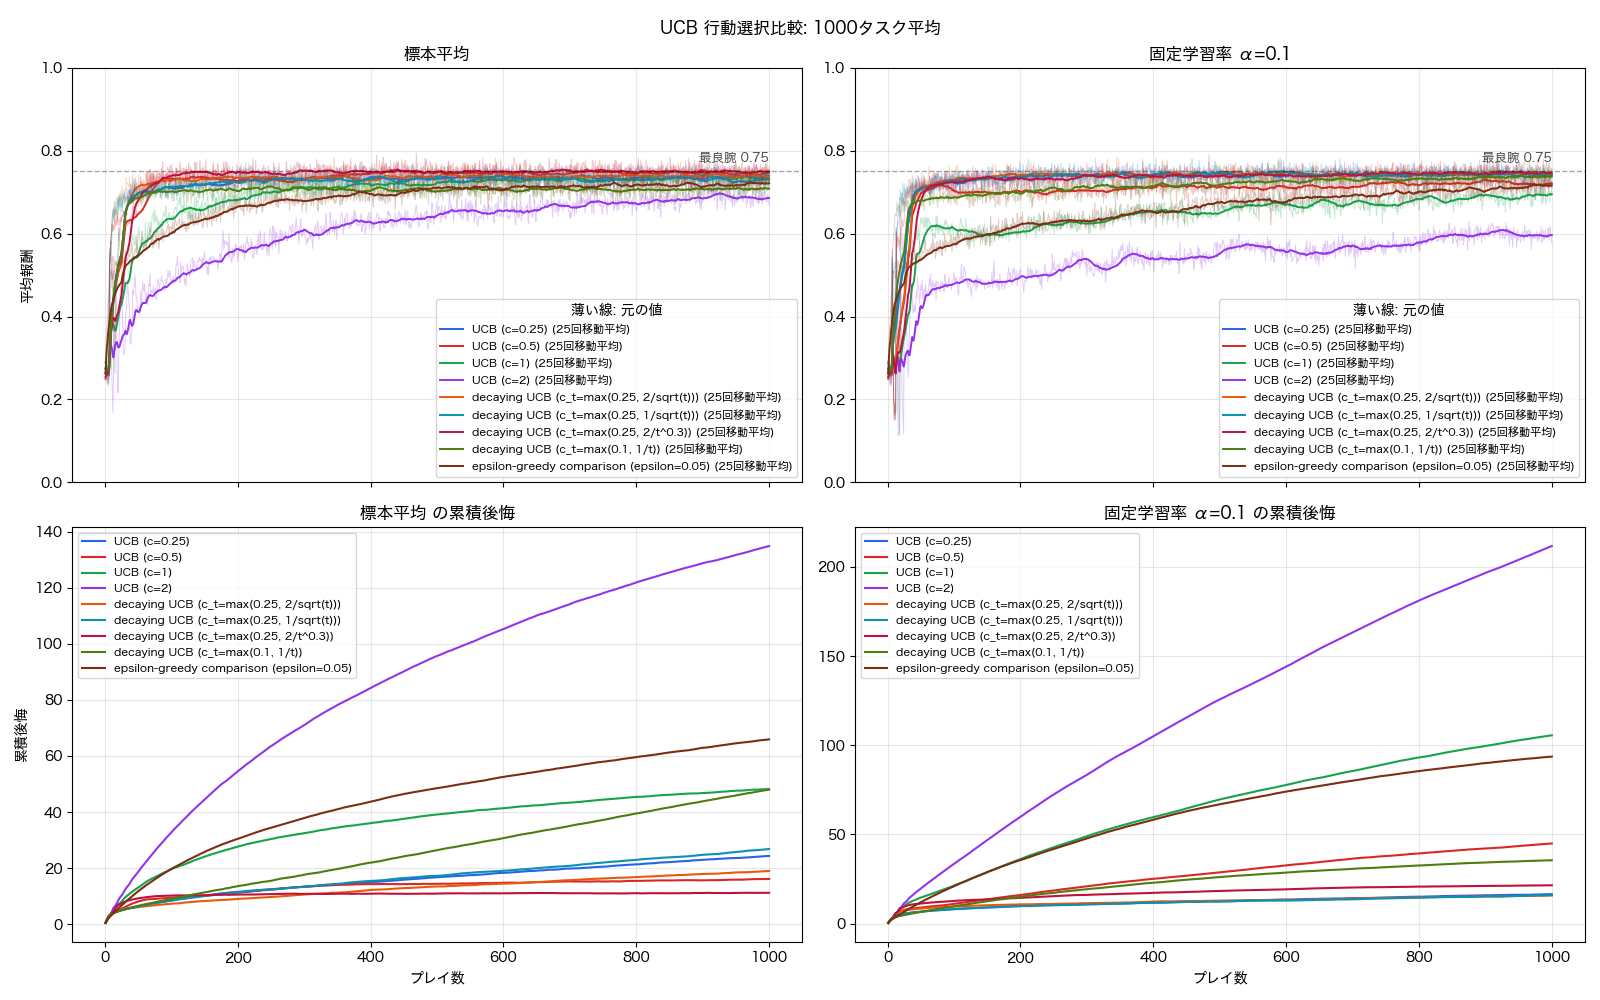
\includegraphics[width=\linewidth]{assets/reinforcement_column/ucb.png}
  \captionof{figure}{UCB 法の学習曲線}
  \label{fig:ucb}
\end{center}

\ \textbf{UCB 法}\\
次に，UCB による行動選択を比較する．
UCB は，現在の推定価値が高い腕だけでなく，
まだ十分に試されていない腕も高く評価する方法である．
具体的には，
\[
    A_t
    =
    \arg\max_{a\in\mathcal{A}}
    \left\{
        Q_t(a)
        +
        c\sqrt{\frac{\log t}{N_t(a)}}
    \right\}
\]
によって腕を選ぶ．
ここで $N_t(a)$ は時刻 $t$ までに腕 $a$ を選んだ回数であり，
$c>0$ は探索ボーナスの強さを決めるパラメータである．
第2項は，選択回数の少ない腕ほど大きくなるため，
UCB は単なるランダム探索ではなく，
\textbf{まだ不確実な腕を意図的に試す}方法と解釈できる．

\ 図\ref{fig:ucb}を見ると，$c$ が大きすぎる場合には性能が悪化している．
特に $c=2$ では平均報酬が低く，累積後悔も大きい．
これは，探索ボーナス
\[
    c\sqrt{\frac{\log t}{N_t(a)}}
\]
が大きすぎるために，すでに低報酬だと分かりつつある腕も繰り返し試してしまうからである．
今回の問題では，最適腕と次善腕の報酬確率差は
\[
    \Delta = p_6-p_5=\frac{1}{4}
\]
である．
したがって，探索ボーナスがこの差 $\Delta$ より十分大きい間は，
第6腕が高い推定価値を持っていても，試行回数の少ない腕が選ばれやすい．
つまり，$c$ が大きすぎると，UCB は慎重すぎる学習者になり，
不確実性を減らすための探索コストが累積後悔として残る．

\ 一方で，$c$ が小さい場合には，探索ボーナスが弱くなり，
現在の推定価値 $Q_t(a)$ をより重視する．
図では，$c=0.25$ や $c=0.5$ が比較的良い結果を示している．
これは，今回の6本腕バンディット問題では報酬確率の差が比較的大きく，
少ない試行回数でも第6腕の有利さを見つけやすかったためだと考えられる．

\ UCB の特徴は，累積後悔の傾きにも現れている．
$c$ が適切な場合，初期には全ての腕を試すために後悔が増えるが，
第6腕が有望であると分かるにつれて選択が集中し，
累積後悔の傾きが小さくなる．
一方，$c=2$ のように探索が強すぎる場合には，
後半になっても低報酬の腕を試す影響が残るため，
累積後悔の傾きが十分に小さくならない．

\ また，時間変化する UCB 係数 $c_t$ も比較した．
これは，学習初期には大きめの探索ボーナスで各腕を広く試し，
学習後半では探索ボーナスを小さくして，
推定価値の高い腕をより重視する方法である．
たとえば
\[
    c_t=\max\left(0.25,\frac{1}{\sqrt{t}}\right)
\]
のように設定すると，初期には強めに探索しつつ，
後半には $c_t$ が下限値 $0.25$ に近づく．
UCB の探索ボーナスそのものは
\[
    c_t\sqrt{\frac{\log t}{N_t(a)}}
\]
であるため，$c_t$ を小さくすることで後半の過剰な探索をさらに抑えられる．
ただし，$c_t$ を小さくしすぎると，
UCB の利点である「試行回数の少ない腕を体系的に試す」効果も弱くなる．
したがって，UCB でも探索の強さを問題のスケールに合わせることが重要である．

\begin{center}
  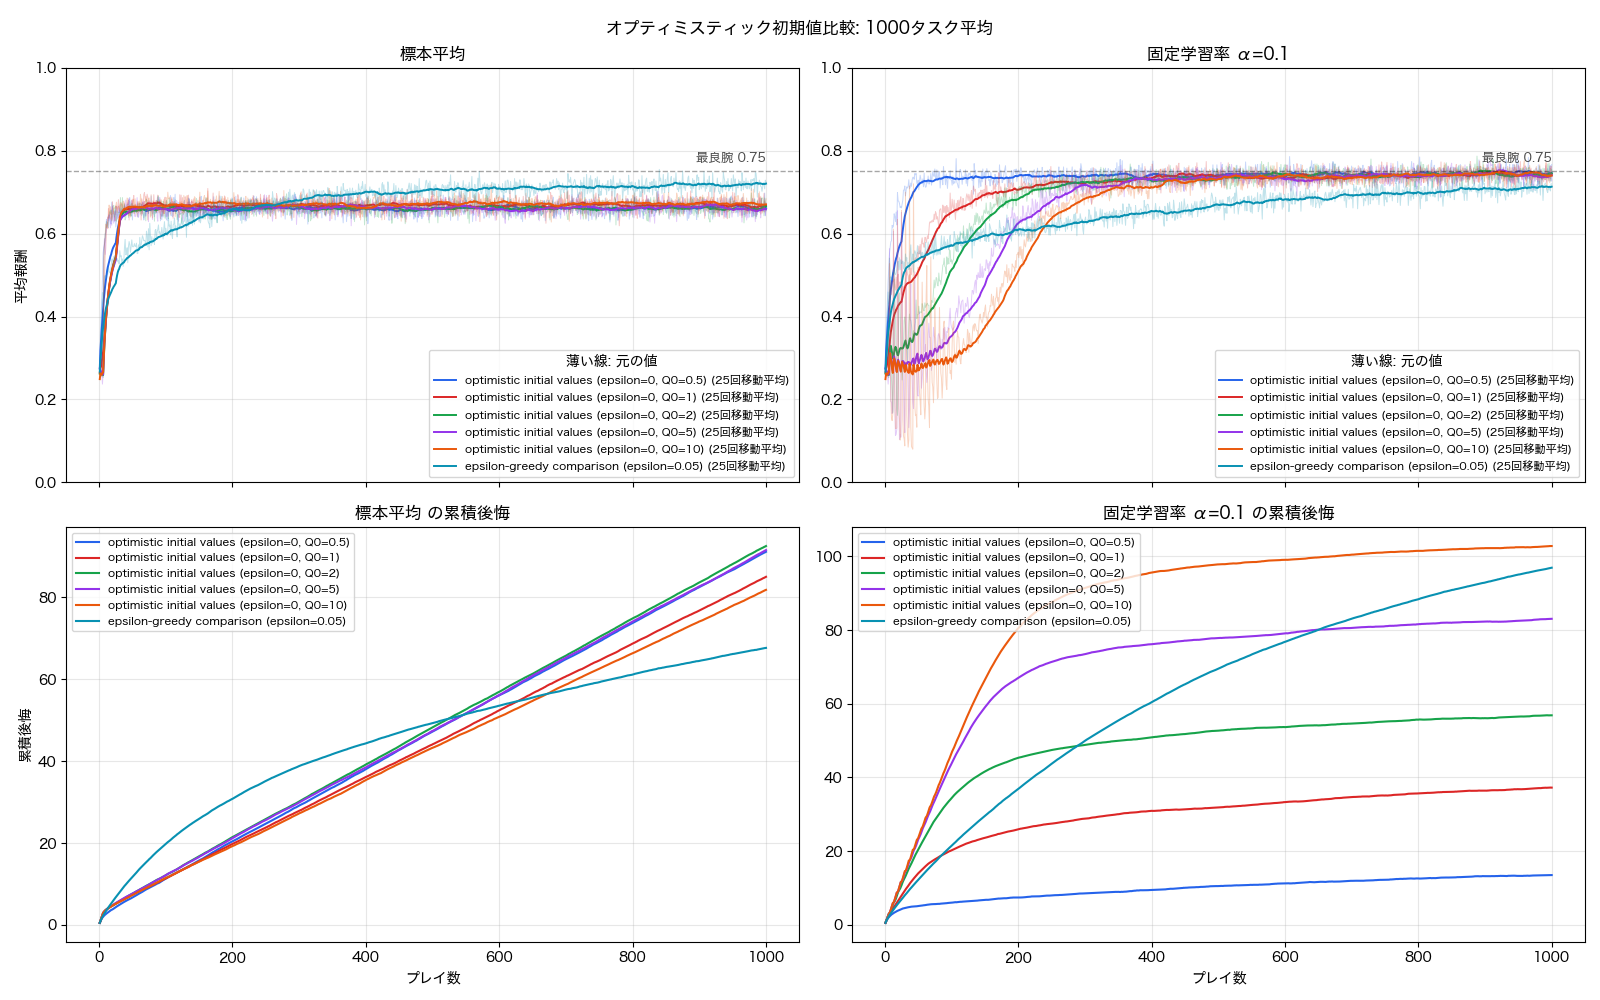
\includegraphics[width=\linewidth]{assets/reinforcement_column/optimistic.png}
  \captionof{figure}{オプティミスティック初期値の学習曲線}
  \label{fig:optimistic}
\end{center}

\ \textbf{optimistic 初期値}\\
次に，optimistic 初期値による探索を比較する．
これは，初期の行動価値 $Q_0(a)$ を高めに設定することで，
まだ十分に試していない腕を魅力的に見せる方法である．
本実験では $\varepsilon=0$ とし，明示的なランダム探索は行わず，
初期値の楽観性だけで探索がどの程度生じるかを調べた．

\ 図\ref{fig:optimistic}を見ると，標本平均を用いた場合には，
$Q_0$ を変えても最終的な結果はどれも似たように悪くなっている．
これは，標本平均手法では，腕 $a$ を初めて選んだ時点で
\[
    Q_1(a)=r_1
\]
となり，初期値 $Q_0(a)$ の影響がほとんど消えてしまうためである．
つまり，$Q_0$ をいくら大きくしても，その腕を一度試すと，
価値推定は実際に得られた $0$ または $1$ の報酬に置き換わる．
そのため，optimistic 初期値は「まだ一度も試していない腕を試させる」
効果は持つが，その後の価値推定には残りにくい．
結果として，標本平均では $Q_0$ の違いが学習曲線に大きく反映されず，
どの初期値でも似た挙動になったと考えられる．

\ 一方，固定学習率 $\alpha=0.1$ を用いた場合には，
初期値によって学習速度に大きな差が現れている．
固定学習率の更新は
\[
    Q_{n}(a)
    =
    (1-\alpha)^n Q_0(a)
    +
    \sum_{i=1}^{n}
    \alpha(1-\alpha)^{n-i}r_i
\]
と展開できる．
この式から分かるように，固定学習率では初期値の影響が
$(1-\alpha)^n Q_0(a)$ として残る．
したがって，$Q_0$ を大きくすると，その腕が何度か低い報酬を出しても，
しばらくは高く評価され続ける．

\ 図では，$Q_0=0.5$ の場合に平均報酬が早く高い値へ到達し，
累積後悔も小さくなっている．
これは，初期値が大きすぎず，初期の探索を促しつつ，
低報酬の腕への過大評価が比較的早く解消されたためだと考えられる．
逆に，$Q_0=5$ や $Q_0=10$ のように初期値が大きすぎると，
低報酬の腕も長い間高く評価され続ける．
たとえば報酬がしばらく $0$ だった場合，固定学習率では
\[
    Q_n(a)=(1-\alpha)^n Q_0(a)
\]
となる．
$\alpha=0.1$ では $(1-\alpha)^n=0.9^n$ なので，
$Q_0$ が大きいほど，その過大評価が十分に下がるまで多くの試行が必要になる．

\ 以上より，optimistic 初期値は，標本平均よりも固定学習率と組み合わせたときに
特徴が現れやすい．
標本平均では初期値が一度の観測でほぼ消えてしまうのに対し，
固定学習率では初期値の影響がしばらく残るため，
初期値の大きさが探索の強さと学習速度を大きく左右する．
ただし，初期値は大きければよいわけではなく，
小さすぎると探索を促せず，大きすぎると悪い腕への過大評価が長く残る．
今回の結果は，optimistic 初期値もまた，
問題の報酬スケールに合わせて設定する必要があることを示している．

\begin{center}
  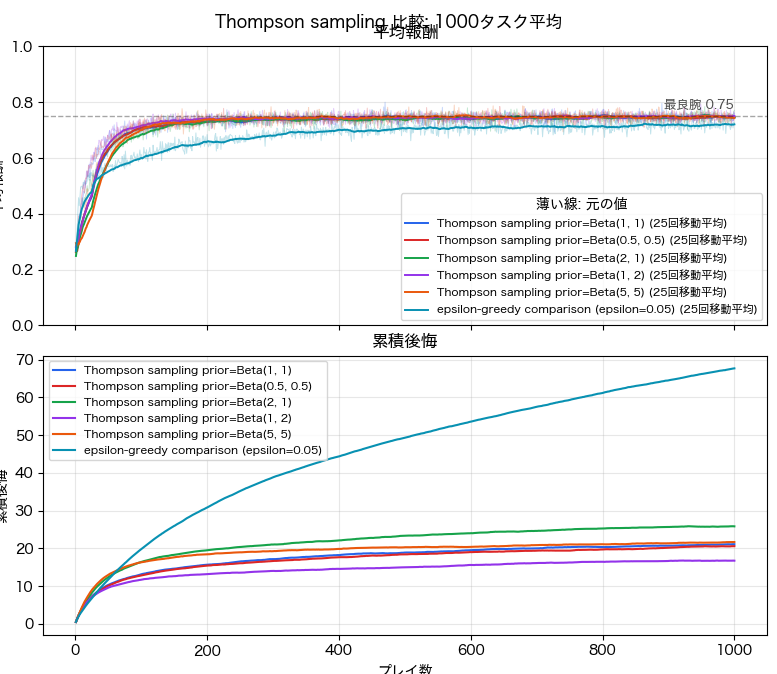
\includegraphics[width=\linewidth]{assets/reinforcement_column/thompson.png}
  \captionof{figure}{Thompson sampling の学習曲線}
  \label{fig:thompson}
\end{center}

\ \textbf{Thompson sampling}\\
最後に，Thompson sampling による行動選択を比較する．
Thompson sampling では，各腕の報酬確率そのものを一点推定するのではなく，
その不確実性を確率分布として保持する．
各時刻では，腕 $a$ の報酬確率に関する事後分布から値をサンプリングし，
そのサンプル値が最大となる腕を選ぶ．

\ 今回の実験では報酬が Bernoulli$(p_a)$ に従うため，
各腕の成功確率 $p_a$ に対してベータ分布を用いる．
時刻 $t$ における腕 $a$ の事後分布を
\[
    p_a \sim \mathrm{Beta}(\alpha_a,\beta_a)
\]
とし，そこから
\[
    \tilde{p}_a \sim \mathrm{Beta}(\alpha_a,\beta_a)
\]
をサンプリングして，
\[
    A_t=\arg\max_{a\in\mathcal{A}}\tilde{p}_a
\]
により腕を選ぶ．
報酬 $1$ が得られた場合は $\alpha_a$ を増やし，
報酬 $0$ が得られた場合は $\beta_a$ を増やす．
したがって，Thompson sampling では，探索は外から加えるランダム行動ではなく，
\textbf{報酬確率に関する不確実性}から自然に生じる．

\ 図\ref{fig:thompson}では，事前分布の違いによる学習曲線の変化を比較している．
ベータ分布 $\mathrm{Beta}(\alpha,\beta)$ の平均は
\[
    \mathbb{E}[p]
    =
    \frac{\alpha}{\alpha+\beta}
\]
であり，$\alpha+\beta$ が大きいほど事前分布は強くなる．
つまり，$(\alpha,\beta)$ は単なる初期値ではなく，
「はじめにどの程度の成功・失敗を仮想的に見たことにするか」を表している．

\ 結果を見ると，Thompson sampling は全体として
$\varepsilon$-greedy の比較対象よりも累積後悔が小さく，
平均報酬も早く高い値に近づいている．
これは，各腕の不確実性を分布として持つことで，
まだ情報が少ない腕には自然に探索の余地が残り，
成功が多く観測された腕には選択が集まりやすくなるためである．

\ 事前分布の違いに注目すると，
$\mathrm{Beta}(1,2)$ が特に小さい累積後悔を示している．
この事前分布の平均は $1/3$ であり，成功確率をやや低めに見積もる悲観的な事前分布である．
今回の問題では低報酬の腕が多いため，成功確率をやや低く見る事前分布は，
低報酬の腕を早めに見切る方向に働きやすい．
その一方で，第6腕のように成功が多く観測される腕では，
事後分布がすぐに高い値へ移動するため，選択が集中しやすい．

\ 一方，$\mathrm{Beta}(2,1)$ は平均 $2/3$ を持つ楽観的な事前分布である．
この場合，各腕の成功確率を初期には高めに見積もるため，
低報酬の腕についても「本当は良い腕かもしれない」という不確実性が残りやすい．
その結果，低報酬の腕を見切るまでにやや時間がかかり，
累積後悔が大きくなりやすい．
これは，optimistic 初期値において初期値を大きくしすぎると
悪い腕への過大評価が長く残ることと似ている．

\ また，$\mathrm{Beta}(0.5,0.5)$ は U 字型の分布であり，
成功確率が $0$ 付近または $1$ 付近にある可能性を比較的大きく見る事前分布である．
そのため，初期にはサンプル値が極端になりやすく，
不確実性に基づく探索がやや強く出る．
一方，$\mathrm{Beta}(5,5)$ は平均 $1/2$ の周辺に集中した事前分布であり，
初期にはどの腕も中程度の成功確率を持つという強めの信念を置く．
この場合，観測が少ない段階では事前分布の影響が残り，
第6腕の優位性を反映するまでに少し時間がかかる．

\ この結果から，Thompson sampling における事前分布は，
単なる初期設定ではなく，探索の性質そのものを決める要素であることが分かる．
中立的な事前分布では観測に素直に反応し，
楽観的な事前分布では探索が長く残りやすく，
悲観的な事前分布では低報酬の腕を早く見切りやすい．
ただし，悲観的すぎる事前分布では本当に良い腕を十分に試す前に
候補から外してしまう危険もあるため，事前分布も問題の報酬スケールに依存して調整される．

\begin{center}
  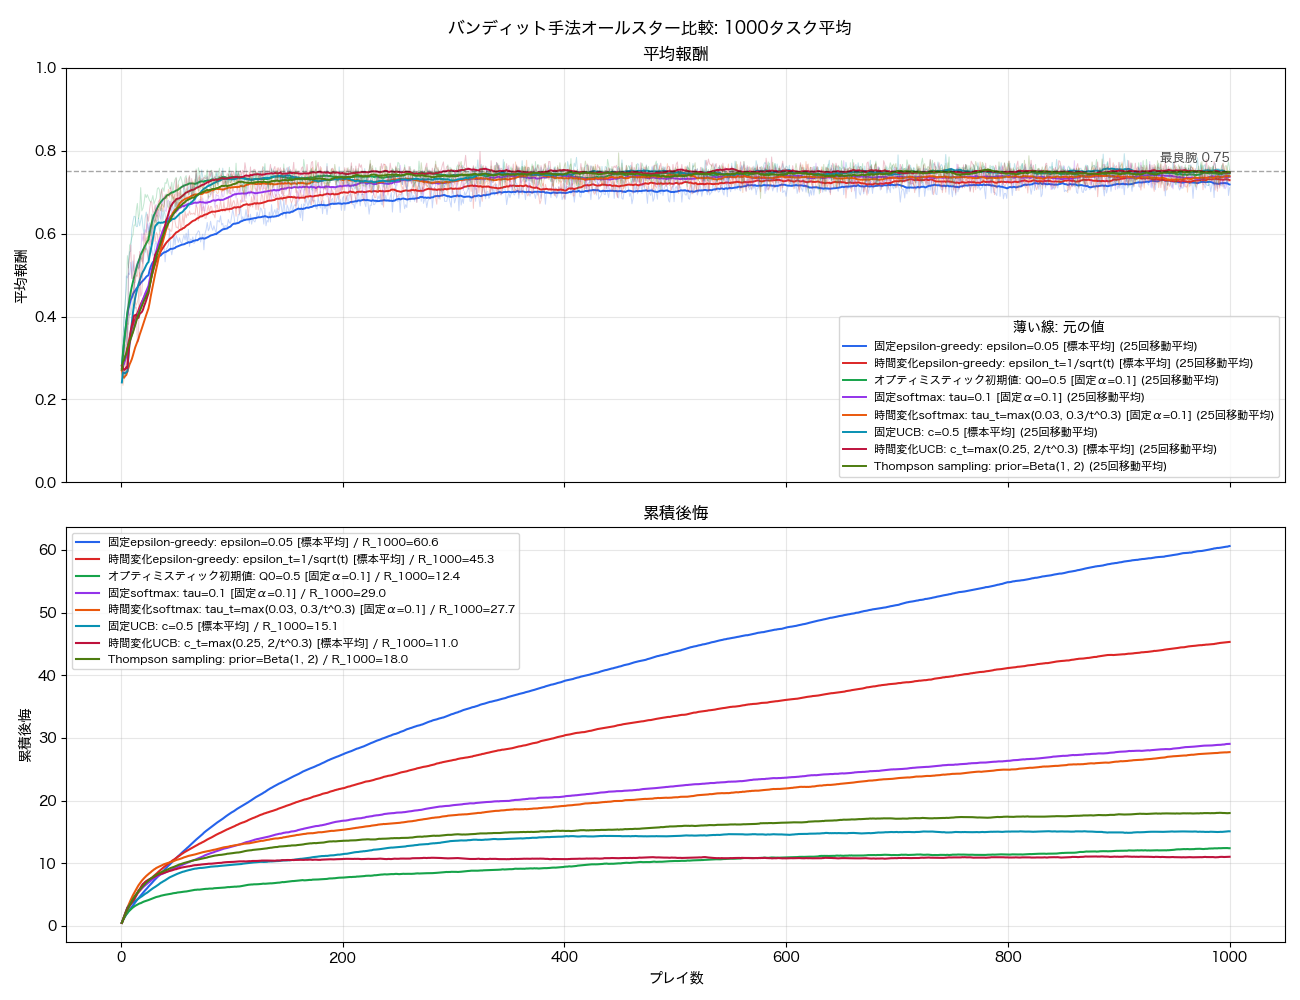
\includegraphics[width=\linewidth]{assets/reinforcement_column/allstar.png}
  \captionof{figure}{全手法の，最も累積後悔が小さくなるようなパラメータでの学習曲線}
  \label{fig:bandit-allstar}
\end{center}

\ \textbf{手法間の比較とまとめ}\\
最後に，各手法について今回の問題で比較的よい性能を示したパラメータを選び，
同一の図で比較した．
図\ref{fig:bandit-allstar}を見ると，平均報酬の推移だけでは，
多くの手法が最終的に最適腕の期待報酬 $0.75$ 付近へ近づいており，
大きな差は見えにくい．
しかし，累積後悔を見ると，各手法の違いはかなり明確に現れる．
これは，平均報酬が「最終的にどこまで到達したか」を見る指標であるのに対し，
累積後悔は「そこに至るまでにどれだけ損をしたか」を記録する指標だからである．

\ 今回の結果では，optimistic 初期値，時間変化する UCB，固定 UCB が特に小さい累積後悔を示している．
optimistic 初期値は，初期価値を高く設定することで未試行の腕を自然に試させるため，
初期の探索を素早く行うことができる．
今回のように定常的で，かつ最適腕と次善腕の差が比較的大きい問題では，
一度よい腕を見つければそのまま活用しやすく，累積後悔が小さくなったと考えられる．
また UCB は，試行回数の少ない腕に探索ボーナスを与えるため，
ランダムに探索するのではなく，不確実な腕を体系的に試すことができる．
その結果，探索の無駄が少なく，早い段階で第6腕へ選択を集中できたと解釈できる．

\ 一方で，固定 $\varepsilon$-greedy は累積後悔が大きくなっている．
これは，最適腕を見つけた後も確率 $\varepsilon$ でランダム探索を続けるためである．
学習が十分に進んだ後の平均報酬は
\[
    (1-\varepsilon)p^\ast
    +
    \varepsilon \frac{1}{K}\sum_{a=1}^{K}p_a
\]
で近似されるため，$\varepsilon>0$ である限り，
低報酬の腕を引く損失が残る．
時間変化する $\varepsilon_t$-greedy は，初期には探索し，
後半には $\varepsilon_t$ を小さくすることでこの問題を緩和している．

\ softmax でも，固定温度では学習後も確率的な選択が残る．
温度 $\tau$ が大きいと探索が残りすぎ，温度が小さいと初期の推定誤差に過敏になる．
今回の比較では，時間変化する softmax は固定 softmax よりよい結果を示しており，
温度を下げながら探索から活用へ移行することの有効性が見られる．
ただし，softmax は価値差を指数関数で選択確率に変換するため，
適切な温度スケールは報酬確率差に強く依存する．
今回うまくいった温度が，他の報酬スケールでもそのまま有効とは限らない．

\ Thompson sampling も比較的良い結果を示している．
探索率や温度を外から指定するのではなく，
各腕の報酬確率に関する事後分布からサンプリングすることで探索が生じるため，
明示的な探索率を設定しなくても，探索と活用のバランスを比較的うまく取ることができたと考えられる．

\ ただし，ここまでの結果は\textbf{定常バンディット問題}における比較である．
各腕の真の報酬確率 $p_a$ が時刻によらず一定であるという仮定のもとでは，
過去の観測を蓄積することに意味があり，
標本平均，UCB，Thompson sampling のように，
観測回数が増えるほど推定を確信していく手法が有効に働きやすい．
しかし，非定常環境では古い観測が現在の環境を表さない可能性がある．
そのため，過去の全データを同じ重みで用いる標本平均手法は，
変化後の最適腕に追従しにくい．

\ この観点から見ると，定常環境で特に意味を持つ手法と，
非定常環境でも活かしやすい手法を分けて考える必要がある．
標本平均に基づく greedy，UCB，通常の Thompson sampling は，
基本的には「真の報酬確率が一定であり，観測を重ねるほど正しい値に近づく」
という考え方に支えられている．
したがって，定常環境では強いが，非定常環境では古い情報を信じすぎる危険がある．
特に UCB では，ある腕を十分に試した後は探索ボーナス
\[
    c\sqrt{\frac{\log t}{N_t(a)}}
\]
が小さくなるため，環境変化後にその腕を再び探索する力は弱くなる．
Thompson sampling でも，観測数が増えて事後分布が鋭くなると，
過去の信念が強く残り，新しい変化に反応しにくくなる場合がある．

\ 一方，固定学習率による価値更新や，探索率・温度・UCB係数を時間変化させる設計は，
非定常環境へ拡張する余地を持つ．
固定学習率では
\[
    Q_n
    =
    (1-\alpha)^nQ_0
    +
    \sum_{i=1}^{n}\alpha(1-\alpha)^{n-i}r_i
\]
となり，最近の報酬ほど大きな重みを持つ．
したがって，古い観測を徐々に忘れながら，新しい環境に追従しやすい．
同様に，非定常環境では探索率を完全には下げきらず，
一定の探索を残すことにも意味がある．
定常環境では不要な探索は後悔を増やすが，
非定常環境では，環境変化を発見するための観測機会になるからである．

\ 以上の比較から，多腕バンディット問題における手法の良し悪しは，
単に平均報酬の高さだけでは判断できないことが分かる．
それぞれの違いは，最適腕をどれだけ早く見つけるか，
低報酬の腕をどれだけ早く見切るか，
そして学習後に不要な探索をどれだけ残すかという形で，
累積後悔の曲線に現れる．

\ 本実験を通じて，多腕バンディット問題は，
強化学習における探索と活用を理解するための最小構成の実験場であることが確認できた．
状態遷移を持たない単純な問題であっても，
探索率，温度，探索ボーナス，初期値，事前分布，学習率の選び方によって，
学習曲線は大きく変化する．
したがって，より複雑な強化学習問題を扱う際にも，
アルゴリズムを名前で選ぶのではなく，
その手法が\textbf{何を不確実とみなし，どのように探索し，どの程度過去を信じるのか}
を考えることが重要である．

\end{column}
\clearpage

\input{chapters/machine_learning/generative_model.tex}
\clearpage
\begin{column}{Persona駆動型LLMによる災害後居住地選択モデル}{三木隆斗}
本章では，生成モデルを「観測データの背後にある構造を仮定し，その構造から観測が生じる」と捉えた．この考え方は，画像や文章の生成だけでなく，人間の選択行動のモデル化にも応用できる．ここでは，津波避難後の居住地選択を，personaを潜在表現として用いるLLMモデルで記述した例を紹介する．焦点は，LLMを単に分類器として使うのではなく，世帯ごとの見えにくい選好や判断基準をpersonaとして表現し，それをloading関数で選択する点にある．

\medskip
\noindent
\textbf{研究背景}

戦争，紛争，巨大災害の後には，被災者の避難，移住，再定住といった長期的な人口移動が発生する．とくに人口減少傾向にある地域では，災害後に誰がどこへ移るかが，その後の地域の人口構成，復興事業の進み方，公共住宅の需要，生活圏の再編に大きく影響する．したがって，災害後の居住地選択を理解することは，復興計画や住宅供給のマネジメントにとって重要である．

一方で，この現象は通常の交通行動モデルより扱いにくい．既存の交通計画理論では，通勤や買物，避難時の移動のように，比較的短期の選択を扱うことが多い．しかし，災害後の移住や定住は数年から数十年単位で進む長期現象であり，次のような難しさがある．

\begin{itemize}
\item 長期的な定量データを得にくい．
\item 世帯ごとの居住履歴が不完全になりやすい．
\item 復興制度，住宅供給，地域条件，家族事情が絡み合う．
\item 観測属性だけでは，帰還意向や再建意欲などの判断基準を捉えにくい．
\end{itemize}

このような背景から，表形式の変数だけでなく，世帯の履歴や地域文脈を文章として扱えるモデルが必要になる．大規模言語モデル（large language model; LLM）は，人間の判断過程を文脈依存的に表現しうるため，従来の離散選択モデルでは表しにくい半構造的な意思決定文脈を入力できる．

\medskip
\noindent
\textbf{使用データ}

使用したデータは，2026年3月に実施された被災者アンケートである．対象は，災害時の居住地域が宮城県・岩手県・福島県のいずれかであった世帯であり，個人属性，世帯属性，居住地選択履歴，住宅類型などの情報を含む．データの規模は次の通りである．

\begin{center}
\scriptsize
\begin{tabular}{lr}
\toprule
項目 & 件数 \\
\midrule
世帯数 & 5,002 \\
各世帯の状態数 & 11,662 \\
居住地移動サンプル数 & 6,660 \\
\bottomrule
\end{tabular}
\end{center}

学習・評価の分割は世帯単位で行った．これは，同一世帯の履歴が訓練データとテストデータにまたがると，履歴情報を通じた情報漏洩が起こりうるためである．LLMによる評価は計算コストが大きいため，テストデータのうち先頭200件を用いた．

\begin{center}
\scriptsize
\begin{tabular}{lrr}
\toprule
分割 & 移動サンプル数 & 世帯サンプル数 \\
\midrule
訓練データ & 4,691 & 3,542 \\
バリデーション & 982 & 709 \\
テスト & 987 & 751 \\
LLM評価 & 200 & 151 \\
\bottomrule
\end{tabular}
\end{center}

\medskip
\noindent
\textbf{予測タスク}

予測タスクは，各世帯の時点 \(t\) までの情報から，次時点 \(t+1\) の居住状態変化を予測する問題である．
\begin{equation}
x_{i,t}=\phi(s_{i,0:t}), \qquad
y_{i,t}=g(s_{i,t},s_{i,t+1}) \in \mathcal{Y}.
\end{equation}
ここで \(x_{i,t}\) は世帯 \(i\) について時点 \(t\) までに観測可能な属性・履歴から作る特徴量，\(s_{i,t}\) は地域，住宅類型，復興段階，時点などを含む居住状態，\(y_{i,t}\) は次状態への遷移を分類したラベルである．将来情報など，予測時点 \(t\) で本来分からない情報は入力から除外した．符号化前の推論時特徴量数は31である．

選択肢集合 \(\mathcal{Y}\) は次の6種類である．

\begin{center}
\scriptsize
\begin{tabular}{lrr}
\toprule
選択肢 & サンプル数 & 比率 \\
\midrule
現在地にとどまる & 519 & 7.8\% \\
被災地域内の仮住まいへ移る & 241 & 3.6\% \\
被災地域外の仮住まいへ移る & 1,676 & 25.2\% \\
災害公営住宅に移る & 340 & 5.1\% \\
自力再建先に移る & 3,286 & 49.3\% \\
帰還する & 598 & 9.0\% \\
\bottomrule
\end{tabular}
\end{center}

この分布から分かるように，「自力再建先に移る」がほぼ半数を占める．したがって，単純に多数派を選ぶモデルでも一定の正解率は出るが，少数クラスを識別できるか，また全体の移動分布を再現できるかが重要になる．

\medskip
\noindent
\textbf{LLMを使う動機}

多項ロジットモデルやニューラルネットワークは，表形式に整理された特徴量を入力として扱う．これに対して，災害後の居住地選択では，「なぜ帰還できないのか」「なぜ仮住まいを継続するのか」「自力再建を選ぶ条件は何か」といった説明的な文脈が重要である．これらは，単純な数値変数だけでは表しきれない．

そこで，LLMへのプロンプトには，世帯属性，居住履歴の文章要約，災害後の地域文脈，仮住まい・帰還・自力再建などの候補説明を含める．さらに，その世帯がどのような判断傾向を持ちそうかを表すpersonaを与える．LLMは，これらの文脈を読んだ上で，6つの選択肢の中から次の居住地選択を出力する．

\medskip
\noindent
\textbf{personaを潜在変数として見る}

personaとは，個票データから直接観測される変数ではなく，世帯の行動傾向や判断基準を文章で要約した潜在表現である．たとえば，同じ「仮住まい中」という状態でも，早期帰還を望む世帯，自力再建を目指す世帯，災害公営住宅を待つ世帯では，次の選択が異なる可能性がある．この差は，年齢や世帯人数のような観測属性だけでなく，生活再建の方針や地域へのこだわりによっても生じる．

生成モデルの記法でいえば，観測された特徴量 \(x\) と選択 \(y\) の背後に，直接観測されないpersona \(m\) があるとみなせる．
\begin{equation}
p(y\mid x)
=
\sum_m p(y\mid x,m)\,p(m\mid x).
\end{equation}
ここで \(p(m\mid x)\) は対象世帯にどのpersonaを割り当てるかを表すloadingであり，\(p(y\mid x,m)\) は，そのpersonaを文脈として与えたLLMが各選択肢を選ぶ分布に対応する．これは，潜在変数モデル
\begin{equation}
p_\theta(x)=\int p_\theta(x\mid z)p(z)\,dz
\end{equation}
において，観測されない \(z\) を周辺化する考え方と対応している．本研究では，personaがこの \(z\) に相当する役割を持つ．

\medskip
\noindent
\textbf{persona bankを用いた推論の流れ}

personaを使った推論は，次の手順で行う．

\begin{enumerate}
\item 訓練データの世帯属性・居住履歴をLLMに与え，世帯の行動傾向を説明するpersonaを作成する．
\item 作成したpersonaをpersona bankとして保存する．
\item 予測対象世帯の属性・履歴から，近いpersonaをloading関数で選ぶ．
\item 現在状態，居住履歴，選択肢説明，選ばれたpersonaをLLMへのプロンプトに入れる．
\item LLMが6つの候補から次の居住地選択を出力する．
\end{enumerate}

重要なのは，personaそのものが最終予測ではない点である．personaは，LLMが文脈依存的な判断を行うための補助的な潜在表現である．したがって，同じpersonaが選ばれても，現在地，履歴，選択肢説明が異なれば，異なるchoiceが出ることが望ましい．

\medskip
\noindent
\textbf{コサイン類似度によるloading}

もっとも単純なloadingは，予測対象世帯とpersona bank内の各personaをベクトル化し，類似度が最大のpersonaを選ぶ方法である．世帯属性や履歴要約をベクトル化する関数を \(\psi(\cdot)\)，persona \(m\) の表現を \(p_m\) とすると，
\begin{equation}
m^*(x)
=
\argmax_m
\operatorname{sim}\{\psi(x),\psi(p_m)\}
\end{equation}
と書ける．コサイン類似度を使う場合，
\begin{equation}
\operatorname{sim}\{\psi(x),\psi(p_m)\}
=
\frac{\psi(x)^\top \psi(p_m)}
{\|\psi(x)\|\|\psi(p_m)\|}
\end{equation}
である．

この方法は直感的で実装しやすい．しかし，属性や履歴が近いpersonaが，選択行動の予測に最も有効とは限らない．たとえば，年齢や家族構成は似ていても，住宅再建への意向や元居住地へのこだわりが異なれば，次の居住地選択は変わりうる．したがって，単純な類似度だけでは，choiceに効くpersonaを選びきれない可能性がある．

\medskip
\noindent
\textbf{EMアルゴリズム的なlearned loading}

そこで，persona割当そのものを観測されない潜在変数の推論問題とみなし，loading関数を学習する．真の「この世帯にはどのpersonaが対応するか」はデータに含まれていない．一方で，各世帯が実際にどの居住地選択をしたかは観測されている．したがって，personaの割当を，観測されたchoiceをよく説明するように更新することが考えられる．

この発想は，EMアルゴリズムに似ている．EMでは，観測されない潜在変数 \(z\) の事後分布をE-stepで推定し，その推定結果を使ってM-stepでモデルパラメータを更新する．ここでは，persona \(m\) が潜在変数に相当し，loading関数が \(p_\alpha(m\mid x)\) を与えると考える．\(\alpha\) はloading関数のパラメータである．

まず，現在のloading関数に基づいて，世帯 \(i\) がpersona \(m\) に対応する重みを計算する．
\begin{equation}
r_{im}
=
p_\alpha(m\mid x_i)
=
\frac{\exp\{\operatorname{sim}_\alpha(x_i,p_m)\}}
{\sum_{m'}\exp\{\operatorname{sim}_\alpha(x_i,p_{m'})\}}.
\end{equation}
これは，各personaに対するsoft assignmentであり，GMMのEMにおける責務 \(\gamma_{nk}\) と似た役割を持つ．これがE-step的な部分である．

次に，LLMまたは選択モデルが，persona \(m\) を与えたときに観測choice \(y_i\) をどれだけ説明できるかを評価する．理想的には，
\begin{equation}
\sum_i \sum_m r_{im}\log p_\theta(y_i\mid x_i,m)
\end{equation}
が大きくなるように，loading関数のパラメータ \(\alpha\) を更新する．これがM-step的な部分である．実装上は，LLMの内部パラメータを直接更新するのではなく，どのpersonaを選ぶと観測choiceへの適合が高くなるかを用いて，類似度関数 \(\operatorname{sim}_\alpha(\cdot,\cdot)\) を調整する．

このlearned loadingは，単に「属性が近いpersona」を選ぶのではなく，「choiceの予測に効くpersona」を選ぼうとする点に特徴がある．生成モデルの言葉でいえば，personaの事後分布 \(p(m\mid x,y)\) を完全には計算できないため，観測choiceを手がかりに近似的にloadingを改善していると解釈できる．

\medskip
\noindent
\textbf{評価指標と比較モデル}

評価には，個票単位の正解率だけでなく，少数クラスや移動分布の再現性を見る指標を用いた．Accuracyは直感的だが，多数派クラスに引っ張られやすい．Macro F1は各選択肢を同じ重みで評価するため，少数クラスを拾えているかを見やすい．また，Share MAEとJSDは，観測された選択肢シェアと予測シェアのずれを見る指標であり，人口移動分布の再現性を評価するために用いた．

\begin{align}
\mathrm{Acc}
&=
\frac{1}{N}\sum_i \mathbf{1}(\hat{y}_i=y_i),\\
\mathrm{MacroF1}
&=
\frac{1}{|\mathcal{Y}|}\sum_{c\in\mathcal{Y}}\mathrm{F1}_c,\\
\mathrm{ShareMAE}
&=
\frac{1}{|\mathcal{Y}|}\sum_{c\in\mathcal{Y}}|\pi_c-\hat{\pi}_c|,\\
\mathrm{JSD}
&=
\frac{1}{2}D_{\mathrm{KL}}(\pi\|m)
+
\frac{1}{2}D_{\mathrm{KL}}(\hat{\pi}\|m),
\qquad
m=\frac{1}{2}(\pi+\hat{\pi}).
\end{align}
ここで \(N\) は評価サンプル数，\(\hat{y}_i\) は予測ラベル，\(\pi_c\) と \(\hat{\pi}_c\) はそれぞれ選択肢 \(c\) の観測シェアと予測シェアである．また，\(\pi\) と \(\hat{\pi}\) は全選択肢にわたる分布，\(m\) はその平均分布であり，JSDは二つの選択肢分布の形のずれを測る．

比較モデルとして，最頻クラスを選ぶMost Frequent，現在地ごとの多数派を選ぶCurrent Area Majority，直近期の遷移シェアを使うRolling Average，ルールベースのDomain Heuristic，多項ロジットモデル（MNL），多層パーセプトロン（NN），そしてpersonaを用いるLLMモデルを用いた．LLMにはQwen2.5-3B-InstructとQwen2.5-7B-Instructを用いた．

\medskip
\noindent
\textbf{実験結果}

まず3Bモデルでは，personaを与えてもchoiceが十分に多様化しなかった．No-Persona LLMではself rebuiltが98\%を占め，Cosine Persona LLMやLearned Persona LLMでもself rebuiltとtemporary withinに強く偏った．この段階では，LLMが文脈を読んで推論しているというより，personaのあてはめや多数派選択に近い挙動になっていた．

一方，7Bモデルでは選択が多様化し，外部一時避難や帰還も出力されるようになった．LLM評価と同じ200件で比較した結果を次に示す．

\begin{center}
\scriptsize
\begin{tabular}{lccccc}
\toprule
モデル & Acc. & F1 & Bal. & MAE & JSD \\
\midrule
7B Learned & 0.755 & 0.442 & 0.443 & 0.024 & 0.005 \\
7B Cosine & 0.735 & 0.316 & 0.385 & 0.022 & 0.008 \\
Area majority & 0.785 & 0.426 & 0.461 & 0.048 & 0.044 \\
MNL & 0.790 & 0.311 & 0.392 & 0.050 & 0.045 \\
NN & 0.725 & 0.317 & 0.388 & 0.050 & 0.047 \\
\bottomrule
\end{tabular}
\end{center}

Accuracyだけを見ると，MNLやArea majorityが高い．しかし，Macro F1では7B Learned loadingが0.442となり，比較モデルの中で最も高かった．また，JSDは0.005であり，選択肢シェアの分布再現性も高かった．これは，learned loadingが少数クラスを含む選択傾向を捉える上で有効であったことを示している．

choice shareを見ると，observedではself rebuiltが0.590，temporary outsideが0.235であったのに対し，learned loadingではself rebuiltが0.635，temporary outsideが0.250となり，全体の分布形状を比較的よく再現していた．LLM評価データには「現在地にとどまる」が含まれていなかったため5択分布での比較になったが，小さいシェアの選択肢も完全には潰れずに残った．

\begin{center}
\scriptsize
\begin{tabular}{lccc}
\toprule
choice & observed & learned & cosine \\
\midrule
public housing & 0.095 & 0.045 & 0.035 \\
self rebuilt & 0.590 & 0.635 & 0.640 \\
temporary outside & 0.235 & 0.250 & 0.245 \\
temporary within & 0.025 & 0.025 & 0.030 \\
return origin & 0.055 & 0.045 & 0.050 \\
\bottomrule
\end{tabular}
\end{center}

\medskip
\noindent
\textbf{persona使用の集中と解釈}

loading方法ごとのpersona使用を見ると，Cosine-onlyでは4種類のpersonaしか使われず，最上位personaが150件（75.0\%）を占めた．Learned loadingでは使用persona数は5種類，最上位personaは114件（57.0\%）であった．数値上はcosineよりやや分散しているが，依然として少数のpersonaに強く集中しており，loading関数によってpersona集中の課題が解決されたとは言い難い．

一方で，learned loadingでは，同一personaでもchoiceが完全には固定されなかった．これは重要である．もし同じpersonaが常に同じchoiceを出すなら，personaは単なるラベルであり，LLMは文脈を読んでいないことになる．しかし，7B learned loadingでは，personaは選択を一意に決めるものではなく，選択傾向の事前分布として働いていた．最終的なchoiceは，personaに加えて，現在状態，居住履歴，元居住地との関係，選択肢説明によって変化した．

\medskip
\noindent
\textbf{考察と課題}

この実験から，LLMを用いた居住地選択モデルには三つの示唆がある．第一に，災害後の居住地選択のような複雑な意思決定では，モデルサイズが結果に大きく影響する．3Bでは選択肢が多数派に偏りやすかったが，7Bでは選択が多様化した．第二に，personaはLLMに文脈依存的な推論を行わせるための潜在表現として有効である．第三に，観測choiceを用いたlearned loadingは予測分布の再現には寄与したが，personaの使用が少数に集中する問題までは十分に解消できなかった．

一方で，課題も多い．プロンプトを少し変えただけで結果が大きく変わるため，prompt設計の頑健性を検証する必要がある．また，learned loadingでもpersona使用はまだ少数に集中しており，十分に多様な潜在表現を使えているとは言い切れない．さらに，LLMがなぜその選択をしたのか，personaのどの記述が判断に効いたのかを検証する解釈性の分析も必要である．

今後は，復興制度，災害公営住宅の供給量，地域の復旧状況などを政策シナリオとして入力し，居住地選択分布がどのように変わるかを調べることが考えられる．その意味で，persona駆動型LLMモデルは，単なる分類器ではなく，潜在表現を介して災害復興の意思決定支援へ接続しうる生成モデル的な枠組みである．
\end{column}
\clearpage


% ==================================================================
% 参考文献
% ==================================================================
\addcontentsline{toc}{section}{参考文献}
\bibliographystyle{stone-ship}
\bibliography{../src/bibliography/machine_learning}

\clearpage
\begin{column}{コラム}
（内容編集のテスト）
\end{column}
\clearpage
\section{強化学習}

強化学習（reinforcement learning）は，環境との相互作用を通じて意思決定規則を学習し，長期的な累積報酬を最大化するための理論である．教師あり学習では入力と正解の対応が与えられ，教師なし学習では観測データの潜在構造の抽出が中心となるのに対し，強化学習では各時刻の行動に対して正解が即座に与えられるとは限らない．ある行動の評価は，その後に続く状態遷移と報酬列を通じて初めて定まり，その意味で遅延報酬を本質に含んでいる．

本章の目標は，強化学習を単なるアルゴリズムの集合としてではなく，確率的環境のもとで価値関数または方策を学習し，累積報酬を最適化する統一理論として理解することである．標準的な教科書的整理としては \citet{SuttonBarto2018} が広く参照されるが，本章ではそれを踏まえつつ，交通・都市工学の逐次意思決定問題にも接続しやすい形で議論を組み立てる．まず歴史的流れから問題意識を整理し，次にマルコフ決定過程によって標準的定式化を与える．そのうえで，多腕バンディット問題によって探索と活用の本質を切り出し，動的計画法，価値ベース手法，方策勾配法へと進む．最後に，標準的な設定だけでは捉えきれない発展的話題を概観する．

\subsection{強化学習の歴史}

強化学習の歴史を学ぶ必要があるのは，この分野が単に高性能な手法を寄せ集めて成立したのではなく，逐次意思決定に固有の困難に対する応答として発展してきたからである．信号制御，車両経路選択，需要応答交通の運行計画のような問題では，現在の行動が将来の混雑や待ち時間を変化させ，評価は複数時刻にまたがって現れる．したがって，入力と正解の対応をそのまま学べばよい教師あり学習とは異なり，行動の価値を試行錯誤から推定しなければならない．

このとき難しさの中心にあるのが，遅延報酬，探索と活用のトレードオフ，そして方策依存のデータ生成である．第一に，最終的な成果にどの行動が寄与したかを識別する信用割当ての問題が生じる．第二に，より良い行動を見つけるためには未知の選択肢を試す探索が必要だが，探索を増やせば当面の報酬は失われる．第三に，データは受動的に与えられるのではなく，学習者自身の行動によって生成される．これらの特徴が，強化学習に独自の理論を要請する．

歴史的源流は，Bellman による動的計画法と最適制御にある\cite{Bellman1957,Puterman1994}．ここで与えられた基本原理は，長期最適化問題を現在の価値と将来の価値の再帰関係として表すベルマン方程式であった．ただし，この枠組みは環境モデル，すなわち状態遷移確率と報酬関数が既知であることを前提としていた．理論的には明快であっても，未知環境から経験を通じて学ぶという強化学習本来の状況には，そのままでは適用できなかった．

この不足を埋めたのが時間差分学習（temporal-difference learning）である．\citet{Sutton1988}は，将来の完全な帰結を待たず，次時刻の価値推定を足場にして現在の価値を更新するブートストラップの考え方を定式化した．これにより，モンテカルロ法のようにエピソード終了まで待たなくても逐次的に価値を学習できるようになった．ベルマン方程式は，解析のための式であるだけでなく，学習更新式の源泉になったのである．

さらに，\citet{WatkinsDayan1992}による Q 学習は，行動価値関数を直接学ぶことで，環境モデルなしに最適方策へ近づく道を与えた．ここで重要なのは，価値推定と制御の問題が統合されたことである．TD 学習が与えられた方策の価値推定を中心にしていたのに対し，Q 学習は最大演算を通じて最適方策そのものを目指した．

状態空間が高次元化すると，表形式の価値関数では表現能力が不足する．この制約を緩和したのが深層強化学習であり，とくに DQN は画像入力から行動価値を学ぶ代表的成功例となった\cite{Mnih2015}．AlphaGo 以降は，価値学習，方策学習，探索，計画を組み合わせる深層強化学習が急速に発展した\cite{Silver2016}．ただし，この発展は流行紹介として理解するべきではない．本質は，既知モデルから未知モデルへ，表形式から関数近似へ，価値推定から方策最適化へと理論の焦点が拡張された点にある．

同時に，価値ベース手法だけでは連続行動空間や確率的方策の直接最適化に限界があることも明らかになった．\citet{Williams1992}に始まる方策勾配法は，方策を直接最適化対象とする考え方を与え，後に Actor-Critic や PPO のような実用的手法へ発展した\cite{Schulman2015,Schulman2017}．この歴史を貫いているのは，強化学習を「環境との相互作用のもとで累積報酬を最大化する確率的意思決定問題」としてどう定式化し，どう近似的に解くかという問いである．次節では，その標準的枠組みとしてマルコフ決定過程を導入する．

\subsection{マルコフ決定過程}

強化学習を厳密に論じるには，何が状態であり，何が行動であり，何が確率的に変化し，何を最大化したいのかを明示する必要がある．そのための標準的枠組みがマルコフ決定過程（Markov decision process; MDP）である．MDP によって，遅延報酬，価値関数，方策最適化という本章の主要概念を一つの数理的言語で記述できる．

\paragraph*{定義}
MDP は，状態空間 $\mathcal{S}$，行動空間 $\mathcal{A}$，遷移確率 $P(s' \mid s,a)$，報酬関数 $r(s,a,s')$，割引率 $\gamma$ からなる組
\begin{equation}
(\mathcal{S}, \mathcal{A}, P, r, \gamma)
\end{equation}
として与えられる．ここで $s \in \mathcal{S}$ は現在状態，$a \in \mathcal{A}$ は現在行動，$s' \in \mathcal{S}$ は次状態を表す．遷移確率 $P(s' \mid s,a)$ は，状態 $s$ で行動 $a$ を選んだときに次状態が $s'$ になる条件付き確率であり，報酬関数 $r(s,a,s')$ はその遷移に対応する即時報酬の期待値である．割引率 $\gamma \in [0,1)$ は，将来報酬をどの程度現在価値として重視するかを表す係数である．

時刻 $t$ に状態 $s_t$ を観測し，行動 $a_t$ を選び，報酬 $r_t$ を受け取って次状態 $s_{t+1}$ へ移るとする．このとき，時刻 $t$ 以降の累積割引報酬，すなわちリターン $G_t$ を
\begin{equation}
G_t = \sum_{k=0}^{\infty} \gamma^k r_{t+k}
\end{equation}
と定義する．添字 $k$ は現在から何ステップ先の報酬かを表し，$\gamma^k$ はその報酬に掛かる割引である．有限ホライズンではこの和は終端時刻までの有限和となり，無限ホライズンでは $\gamma < 1$ によって収束が保証される．

MDP の核心はマルコフ性にある．これは，次状態と次報酬の条件付き分布が，過去全体ではなく現在状態と現在行動だけで決まるという仮定であり，
\begin{equation}
\mathbb{P}(s_{t+1},r_t \mid s_0,a_0,\ldots,s_t,a_t)
=
\mathbb{P}(s_{t+1},r_t \mid s_t,a_t)
\end{equation}
と書ける．この仮定が重要なのは，現在状態が将来予測に必要な情報を十分に要約しているとみなせるからである．その結果，長期最適化問題を再帰式として記述できる．

\paragraph*{定義}
方策（policy）$\pi(a \mid s)$ は，状態 $s$ のもとで行動 $a$ を選ぶ条件付き確率である．決定論的方策では各状態に一つの行動が対応し，確率的方策では複数の行動に確率が割り当てられる．方策 $\pi$ が与えられたとき，状態価値関数（state-value function）$V^\pi(s)$ と行動価値関数（action-value function）$Q^\pi(s,a)$ を
\begin{align}
V^\pi(s) &= \mathbb{E}_\pi[G_t \mid s_t=s], \\
Q^\pi(s,a) &= \mathbb{E}_\pi[G_t \mid s_t=s, a_t=a]
\end{align}
と定義する．$\mathbb{E}_\pi[\cdot]$ は，方策 $\pi$ と遷移確率 $P$ のもとでの期待値である．$V^\pi(s)$ は状態 $s$ にいることの長期的な良さを，$Q^\pi(s,a)$ は状態 $s$ で行動 $a$ を取ることの長期的な良さを表す．

これらの価値関数は，ベルマン期待方程式を満たす．状態価値関数については
\begin{align}
V^\pi(s)
&=
\sum_{a \in \mathcal{A}} \pi(a \mid s)
\sum_{s' \in \mathcal{S}} P(s' \mid s,a)
\left[
r(s,a,s') + \gamma V^\pi(s')
\right]
\end{align}
が成り立つ．同様に，行動価値関数は
\begin{align}
Q^\pi(s,a)
&=
\sum_{s' \in \mathcal{S}} P(s' \mid s,a)
\left[
r(s,a,s') + \gamma \sum_{a' \in \mathcal{A}} \pi(a' \mid s') Q^\pi(s',a')
\right]
\end{align}
を満たす．ここで $a' \in \mathcal{A}$ は次状態 $s'$ における次の行動である．価値が即時報酬と将来価値の和として再帰的に分解されることが，強化学習の理論的出発点である．

最適方策 $\pi^\ast$ は，全状態で価値を最大化する方策として定義される．対応する最適状態価値関数 $V^\ast(s)$ と最適行動価値関数 $Q^\ast(s,a)$ は
\begin{align}
V^\ast(s) &= \max_\pi V^\pi(s), \\
Q^\ast(s,a) &= \max_\pi Q^\pi(s,a)
\end{align}
であり，ベルマン最適方程式
\begin{align}
V^\ast(s)
&=
\max_{a \in \mathcal{A}}
\sum_{s' \in \mathcal{S}} P(s' \mid s,a)
\left[
r(s,a,s') + \gamma V^\ast(s')
\right], \\
Q^\ast(s,a)
&=
\sum_{s' \in \mathcal{S}} P(s' \mid s,a)
\left[
r(s,a,s') + \gamma \max_{a' \in \mathcal{A}} Q^\ast(s',a')
\right]
\end{align}
を満たす．最大演算は，将来にわたって最も価値の高い行動を選ぶという最適制御の原理を表している．

有限ホライズンと無限ホライズン，エピソード型と継続型の区別も重要である．有限ホライズンでは終端時刻が存在し，無限ホライズンでは割引率が重要になる．エピソード型では終端状態に達すると課題が終了するのに対し，継続型ではタスクが終わらないため，交通流制御のような問題では長期的安定性をどう定義するかが論点になる．次節では，状態遷移という複雑さを一度外し，探索と活用の本質だけを切り出した多腕バンディット問題を考える．

\subsection{多腕バンディット問題}\label{subsec:bandit}

MDP は強化学習の標準形であるが，状態遷移まで含めると探索と活用の本質が見えにくくなることがある．そこで，多腕バンディット問題（multi-armed bandit problem）を導入する．これは状態遷移を持たず，未知の行動価値を試行錯誤によって学ぶという構造だけを残した問題であり，強化学習の基礎概念を理解するうえで有用である\cite{Auer2002,LattimoreSzepesvari2020}．

\paragraph*{定義}
$K$ 本の腕を持つバンディットを考える．各腕 $i \in \{1,\ldots,K\}$ を選ぶと，未知分布に従う報酬が得られ，その期待値を $\mu_i$ とする．時刻 $t$ に選ばれる腕を $A_t$，得られる報酬を $r_t$ と書く．この問題には状態遷移がなく，意思決定は「次にどの腕を引くか」だけである．最適腕の期待報酬を $\mu^\ast=\max_i \mu_i$ とすると，目標は時刻 $T$ までの累積期待報酬を最大化することである．

このとき，性能評価には後悔（regret）がよく用いられる．累積後悔 $R_T$ を
\begin{equation}
R_T
=
T \mu^\ast - \mathbb{E}\left[\sum_{t=1}^{T} r_t\right]
\end{equation}
と定義すると，これは「常に最適腕だけを引いた場合に比べてどれだけ損をしたか」を表す．強化学習全体では累積報酬最大化が中心目的であるが，バンディットでは後悔最小化の形で理論解析が明確になる．

最も単純な戦略の一つが $\epsilon$-greedy である．これは確率 $1-\epsilon$ で現在までに推定された最良の腕を選び，確率 $\epsilon$ で一様ランダムに探索する方法である．ここで $\epsilon \in [0,1]$ は探索率を表す．直感的には，既知の有望な腕を主に活用しつつ，未知の腕をときどき試すことで誤った早期収束を防ぐ．ただし，不確実性の大きさを腕ごとに使い分けないため，探索の効率は高くない．

これに対して，上側信頼限界法（upper confidence bound; UCB）は，推定平均と不確かさの両方を用いる\cite{Auer2002}．腕 $i$ の時刻 $t-1$ までの経験平均を $\hat{\mu}_i(t-1)$，その腕を選んだ回数を $N_i(t-1)$ とすると，典型的には
\begin{equation}
A_t
=
\mathop{\mathrm{arg\,max}}_i
\left[
\hat{\mu}_i(t-1)
+
c \sqrt{\frac{\log t}{N_i(t-1)}}
\right]
\end{equation}
で腕を選ぶ．ここで $c>0$ は探索の強さを調整する定数である．右辺第二項は未観測性に対応し，試行回数が少ない腕ほど大きくなる．したがって UCB は，「現在よさそうな腕」だけでなく「まだ十分試していないので本当は良いかもしれない腕」も積極的に選ぶ．

もう一つの代表的方法が Thompson sampling である\cite{Thompson1933}．これは，各腕の平均報酬に関する事後分布を持ち，そこから仮想的な平均報酬 $\tilde{\mu}_i$ をサンプルして
\begin{equation}
A_t = \mathop{\mathrm{arg\,max}}_i \tilde{\mu}_i
\end{equation}
とする方法である．たとえばベルヌーイ報酬では，成功確率にベータ分布を置くことで計算が容易になる．Thompson sampling の特徴は，探索が外的なランダム化としてではなく，パラメータ不確実性のベイズ的表現から自然に導かれる点にある．

バンディット問題が MDP より簡単なのは，状態遷移がないため，長期的な信用割当てを考える必要がないからである．一方で，本質的に共通している点も明確である．すなわち，未知の環境で累積報酬を最大化するには，不確実性のもとで探索と活用を両立させなければならない．この意味で，多腕バンディットは強化学習の縮約版である．次節では，再び状態遷移を導入し，ただし環境モデルが既知である場合の計画法として動的計画法を扱う．

\subsection{動的計画法}

動的計画法（dynamic programming）が必要になるのは，環境モデルが既知であれば，経験から学ぶ前に理論上の最適解を計算できるからである．これは現実にはしばしば非現実的な仮定であるが，強化学習アルゴリズムの基準点としてきわめて重要である．モデル未知の場合の TD 学習や Q 学習は，多くの場合この枠組みをサンプル近似したものと理解できる．

\paragraph*{定義}
方策 $\pi$ に対するベルマン作用素 $T^\pi$ を
\begin{equation}
(T^\pi V)(s)
=
\sum_{a \in \mathcal{A}} \pi(a \mid s)
\sum_{s' \in \mathcal{S}} P(s' \mid s,a)
\left[
r(s,a,s') + \gamma V(s')
\right]
\end{equation}
と定義する．ここで $V$ は任意の状態価値関数である．同様に，最適ベルマン作用素 $T_\ast$ を
\begin{equation}
(T_\ast V)(s)
=
\max_{a \in \mathcal{A}}
\sum_{s' \in \mathcal{S}} P(s' \mid s,a)
\left[
r(s,a,s') + \gamma V(s')
\right]
\end{equation}
と定義する．ベルマン期待方程式は $V^\pi = T^\pi V^\pi$，ベルマン最適方程式は $V^\ast = T_\ast V^\ast$ という不動点方程式になる．

\paragraph*{アルゴリズム}
方策評価（policy evaluation）は，固定された方策 $\pi$ の価値関数 $V^\pi$ を求める手続きである．初期関数 $V_0$ を任意に取り，
\begin{equation}
V_{k+1} = T^\pi V_k
\end{equation}
と反復すると，$V_k$ は $V^\pi$ に近づく．直感的には，価値は終端報酬や高報酬状態から逆向きに伝播する．まず 1 ステップ先の価値が更新され，その情報がさらに前の状態へ波及していくのである．

方策改善（policy improvement）は，現在の価値関数にもとづいてより良い行動を選ぶ段階である．すなわち，各状態 $s$ について
\begin{equation}
\pi'(s)
\in
\mathop{\mathrm{arg\,max}}_{a \in \mathcal{A}}
\sum_{s' \in \mathcal{S}} P(s' \mid s,a)
\left[
r(s,a,s') + \gamma V^\pi(s')
\right]
\end{equation}
とすれば，新しい方策 $\pi'$ は少なくとも $\pi$ と同程度，通常はそれ以上の価値を持つ．これは，現在の価値評価に照らして各状態で最善の 1 ステップ行動を選べば，方策全体が改善することを意味している．

方策反復（policy iteration）は，方策評価と方策改善を交互に行う方法である．
\begin{enumerate}
\item 現在の方策 $\pi_k$ を評価して $V^{\pi_k}$ を求める．
\item $V^{\pi_k}$ に対して貪欲化を行い，新しい方策 $\pi_{k+1}$ を得る．
\item 方策が変化しなくなるまで反復する．
\end{enumerate}

価値反復（value iteration）は，方策評価を完全に解かずに最適ベルマン作用素を直接適用する方法であり，
\begin{equation}
V_{k+1} = T_\ast V_k
\end{equation}
を反復する．その後，各状態で価値を最大化する行動を選べば最適方策が得られる．価値反復は「いま分かっている将来価値に照らして最善の 1 ステップ選択」を毎回価値へ織り込む方法であり，計画と改善が一体化されている．

\paragraph*{定理}
ベルマン作用素が収束をもたらす理由は，割引率 $\gamma < 1$ のもとで縮小写像になるからである．最大ノルム $\|V-W\|_\infty = \max_{s \in \mathcal{S}} |V(s)-W(s)|$ を用いると，
\begin{align}
\|T^\pi V - T^\pi W\|_\infty &\le \gamma \|V-W\|_\infty, \\
\|T_\ast V - T_\ast W\|_\infty &\le \gamma \|V-W\|_\infty
\end{align}
が成り立つ．誤差が反復ごとに少なくとも $\gamma$ 倍に縮むため，不動点に向かって収束する．直感的には，遠い将来の影響が割引によって弱まり，誤差が増幅しないことを意味する．

動的計画法は理論上の理想解法である一方，遷移確率と報酬関数が既知でなければ使えない．そのため，モデル未知の状況では期待値計算を実際の観測遷移で置き換える必要がある．次節では，その橋渡しとして TD 学習から Q 学習へ至る価値ベース手法を扱う．

\subsection{価値ベース手法：Q学習, Deep-Q学習}

現実の強化学習では，環境モデルが未知であることが多い．したがって，動的計画法のように遷移確率の期待値を厳密に計算することはできず，経験から価値を学習しなければならない．価値ベース手法は，価値関数を学ぶことを通じて最適方策を間接的に得る方法であり，モデル未知環境における強化学習の中心的流儀である．

出発点となるのは TD 学習である．状態価値関数 $V$ に対する TD(0) の更新は
\begin{equation}
V(s_t)
\leftarrow
V(s_t) + \alpha
\left[
r_t + \gamma V(s_{t+1}) - V(s_t)
\right]
\end{equation}
で与えられる．ここで $\alpha \in (0,1]$ は学習率である．角括弧内の量
\begin{equation}
\delta_t = r_t + \gamma V(s_{t+1}) - V(s_t)
\end{equation}
を TD 誤差という．$\delta_t$ は，現在の価値予測が 1 ステップ先の観測を踏まえてどれだけ過小または過大であったかを示す量であり，価値修正の方向と大きさを与える信号である．

制御問題では，状態そのものの価値だけでなく，各行動の価値を知る必要がある．そこで行動価値関数 $Q(s,a)$ を学習する．Q 学習は
\begin{equation}
Q(s_t,a_t) \leftarrow Q(s_t,a_t) + \alpha \left[r_t + \gamma \max_{a'} Q(s_{t+1},a') - Q(s_t,a_t)\right]
\end{equation}
という更新式で定義される\cite{WatkinsDayan1992}．ここで $a' \in \mathcal{A}$ は次状態 $s_{t+1}$ における候補行動であり，$\max_{a'} Q(s_{t+1},a')$ は将来に最善行動を選ぶと仮定した価値である．この最大演算を通じて，Q 学習は最適方策へ向かう．

Q 学習の重要な特徴は off-policy 学習である点にある．すなわち，実際にデータを収集する行動方策と，更新式の内部で想定している目標方策が一致していなくてもよい．たとえば $\epsilon$-greedy によって探索を行いながら，更新時には貪欲方策を想定できる．これに対し SARSA は
\begin{equation}
Q(s_t,a_t)
\leftarrow
Q(s_t,a_t) + \alpha
\left[
r_t + \gamma Q(s_{t+1},a_{t+1}) - Q(s_t,a_t)
\right]
\end{equation}
と，実際に選ばれた次行動 $a_{t+1}$ を用いて更新する on-policy 手法である．Q 学習が将来の最良行動に基づく強気の更新であるのに対し，SARSA は探索を含んだ現在の方策をそのまま評価する．

表形式の Q 学習は，状態空間と行動空間が小さいときには有効であるが，高次元状態では破綻する．画像入力や多数の交通状態特徴量のような状況では，各 $(s,a)$ に対して表を持つことができない．このとき必要になるのが関数近似であり，Deep Q-Network（DQN）はニューラルネットワーク $Q(s,a;\theta)$ によって行動価値関数を近似する\cite{Mnih2015}．

DQN では，TD ターゲットを
\begin{equation}
y_t = r_t + \gamma \max_{a'} Q(s_{t+1},a';\theta^-)
\end{equation}
と置き，損失関数
\begin{equation}
L_t(\theta)
=
\left[
y_t - Q(s_t,a_t;\theta)
\right]^2
\end{equation}
を最小化する．ここで $\theta$ は学習中のネットワークの重み，$\theta^-$ はターゲットネットワークの重みである．もし右辺のターゲットまで同じ重みで毎回更新すると，目標そのものが激しく動くため学習が不安定化する．ターゲットネットワークはこの問題を緩和し，更新先を一時的に固定する役割を果たす．

もう一つの重要要素が経験再生（experience replay）である．これは，過去の遷移 $(s_t,a_t,r_t,s_{t+1})$ をバッファに蓄積し，そこから無作為にミニバッチを抽出して学習する仕組みである．経験再生が必要なのは，連続する遷移が強く相関しているため，そのまま学習すると勾配推定が不安定になるからである．無作為抽出により相関を弱められ，同じ経験を複数回再利用できるのでデータ効率も向上する．DQN の安定化は，この経験再生とターゲットネットワークに大きく依存している．

その後，Double DQN は最大演算に由来する過大評価を軽減し，dueling network は状態価値とアドバンテージを分離して表現することで学習効率を高めた．しかし中心的な論点は，TD 学習の再帰構造を深層関数近似とどう両立させるかにある．価値ベース手法の長所は，離散行動空間では各行動の価値を直接比較できること，ベルマン方程式との結びつきが明瞭であることである．一方で，連続行動空間では $\max_{a'} Q(s_{t+1},a')$ の計算が難しく，確率的方策の直接制御や制約付き最適化にも不向きである．この限界が，次節で扱う方策勾配法の必要性を生む．

\subsection{方策勾配法：Actor-Critic, PPO}

価値ベース手法の限界が明確になるのは，連続行動空間や確率的方策の直接最適化を考えるときである．ロボット制御のように行動が実数ベクトルで表される場合，離散行動に対する最大化は自然ではない．また，探索を方策の分布そのものに埋め込みたい場合には，価値関数を介した間接的な最適化より，方策を直接最適化する方が適切である．この問題意識から方策勾配法が導入される．

パラメータ $\theta$ を持つ方策を $\pi_\theta(a \mid s)$ とし，期待リターンを
\begin{equation}
J(\theta) = \mathbb{E}_{\pi_\theta}[G_0]
\end{equation}
と定義する．ここで $\mathbb{E}_{\pi_\theta}[\cdot]$ は，方策 $\pi_\theta$ と環境ダイナミクスに従って生成される軌道に関する期待値である．方策勾配法の目標は，$J(\theta)$ を最大化するように $\theta$ を更新することである．

\paragraph*{定理}
方策勾配の基本形は
\begin{equation}
\nabla_\theta J(\theta) = \mathbb{E}\left[\nabla_\theta \log \pi_\theta(a_t|s_t)\, G_t\right]
\end{equation}
で与えられる\cite{Williams1992}．ここで $\nabla_\theta$ はパラメータ $\theta$ に関する勾配，$\log \pi_\theta(a_t \mid s_t)$ は選択された行動の対数確率，$G_t$ は時刻 $t$ 以降のリターンである．この式は，良い帰結をもたらした行動の確率を高め，悪い帰結をもたらした行動の確率を下げるという学習規則を正当化する．

REINFORCE はこの勾配を標本平均で近似する最も基本的なアルゴリズムであり，
\begin{equation}
\theta \leftarrow \theta + \alpha \sum_t \nabla_\theta \log \pi_\theta(a_t \mid s_t) G_t
\end{equation}
と更新する．ここで $\alpha$ は学習率である．REINFORCE は不偏推定量を与えるが，$G_t$ の分散が大きく，学習が不安定になりやすい．とくにホライズンが長い問題では，分散の削減が不可欠になる．

そこでベースライン $b(s_t)$ を導入し，
\begin{equation}
\nabla_\theta J(\theta)
=
\mathbb{E}\left[
\nabla_\theta \log \pi_\theta(a_t \mid s_t)
\left(G_t - b(s_t)\right)
\right]
\end{equation}
と書き換える．$b(s_t)$ が状態のみに依存する限り，勾配の期待値は変わらず，分散だけを減らせる．とくに $b(s_t)=V^\pi(s_t)$ と置くと，アドバンテージ関数
\begin{equation}
A^\pi(s_t,a_t) = Q^\pi(s_t,a_t) - V^\pi(s_t)
\end{equation}
が現れる．これは，状態 $s_t$ において行動 $a_t$ が平均的行動よりどれだけ良かったかを表す量である．

Actor-Critic はこの考え方を実装する枠組みである．Actor は方策 $\pi_\theta(a \mid s)$ を表し，Critic は価値関数，典型的には $V(s;w)$ を推定する．ここで $w$ は Critic のパラメータである．Critic は TD 学習により
\begin{equation}
\delta_t = r_t + \gamma V(s_{t+1};w) - V(s_t;w)
\end{equation}
を計算する．この TD 誤差 $\delta_t$ は，1 ステップのアドバンテージ推定として機能する．したがって Actor は
\begin{equation}
\theta \leftarrow \theta + \alpha \, \delta_t \, \nabla_\theta \log \pi_\theta(a_t \mid s_t)
\end{equation}
と更新できる．$\delta_t$ が正なら行動確率を増やし，負なら減らすので，Critic の価値推定が Actor の改善方向を与えることになる．

実際の深層強化学習では，方策更新が大きすぎると性能が急激に悪化することがある．TRPO は新旧方策の距離に制約を課すことでこの問題に対処したが\cite{Schulman2015}，計算は比較的重い．これに対し PPO は，同じ問題意識をより簡潔な目的関数で扱う\cite{Schulman2017}．

PPO では，古い方策を $\pi_{\theta_{\mathrm{old}}}$，新しい方策を $\pi_\theta$ とし，確率比
\begin{equation}
r_t(\theta)
=
\frac{\pi_\theta(a_t \mid s_t)}{\pi_{\theta_{\mathrm{old}}}(a_t \mid s_t)}
\end{equation}
を考える．さらに $A_t$ を推定アドバンテージとすると，clip された目的関数は
\begin{equation}
L^{\mathrm{clip}}(\theta)
=
\mathbb{E}
\left[
\min\left(
r_t(\theta)A_t,\,
\mathrm{clip}\left(r_t(\theta),1-\epsilon,1+\epsilon\right)A_t
\right)
\right]
\end{equation}
と書かれる．ここで $\epsilon > 0$ は更新幅を制御するハイパーパラメータであり，$\mathrm{clip}(\cdot)$ は値を区間 $[1-\epsilon,1+\epsilon]$ に切り詰める演算である．新方策が旧方策から過度に離れると，利得の増加が頭打ちになるため，大きすぎる更新が抑制される．

PPO が実用上の標準手法とみなされるのは，信頼領域の思想を保ちつつ，実装が容易でミニバッチ最適化とも相性がよいからである．とくに連続行動空間，大規模関数近似，確率的方策の直接制御が必要な問題では，方策勾配法の重要性は大きい．価値ベース手法が価値推定を通じて行動を導くのに対し，方策勾配法は望ましい行動分布そのものを直接整形する．この違いが，現代の深層強化学習における両者の役割分担を定めている．

\subsection{発展的話題}

標準的な MDP，価値学習，方策勾配法は強力な枠組みであるが，現実世界の課題をそのまま捉えられるわけではない．実応用では，環境モデルは未知であり，観測は不完全であり，安全制約があり，データ収集が高価であることが多い．この節では，そのような制約のもとで基本理論がどのように拡張されるかを概観する．

\subsubsection{モデルベース強化学習}

モデルベース強化学習（model-based RL）が必要になるのは，サンプル効率を高めたいからである．モデルフリー手法は柔軟であるが，多数の試行を要する．実機ロボットや都市交通制御では，試行そのものが高価であり，環境モデルを全く使わない学習は非現実的であることが多い．

基本的な発想は，遷移モデル $\hat{P}$ と報酬モデル $\hat{r}$ をデータから学習し，その近似モデルの内部で計画やロールアウトを行うことである．モデルが十分正確なら，実環境での試行を減らしつつ方策改善ができる．一方で，モデル誤差は長期予測で蓄積しやすいため，短い計画区間に限定する，モデル不確実性を推定する，モデルフリー更新と併用するといった工夫が必要になる．

\subsubsection{オフライン強化学習}

オフライン強化学習（offline RL）が必要になるのは，新たな探索を現場で行えない状況があるからである．医療，金融，公共交通運用のような領域では，学習のために試しに危険な行動を取ることは許されない．そのため，過去に収集された固定データ集合
\begin{equation}
\mathcal{D} = \{(s,a,r,s')\}
\end{equation}
だけを用いて方策を学習する．

ここでの難しさは，データに含まれていない行動を価値関数が過大評価しやすい点にある．すなわち，分布外の行動に対する楽観主義が性能劣化を招く．このため，オフライン強化学習では，行動方策に近い範囲で保守的に学習する，価値推定を意図的に低めに補正する，行動分布そのものを制約する，といった工夫が中心課題となる．

\subsubsection{部分観測 MDP}

標準的 MDP では現在状態が将来予測に必要な情報を十分含むと仮定したが，現実には状態そのものが直接観測できないことが多い．部分観測 MDP（partially observable MDP; POMDP）は，この状況を扱うための拡張であり，エージェントは状態 $s_t$ の代わりに観測 $o_t$ だけを得る．

このとき単一の観測だけでは意思決定に必要な情報が不足することがある．たとえば需要の潜在状態や他主体の意図は直接見えない．そこで，過去観測から信念状態を更新して隠れ状態の分布を内部状態として扱う方法や，再帰型ネットワークによって観測履歴を潜在表現へ圧縮する方法が用いられる．POMDP は，マルコフ性を放棄するのではなく，観測から実質的なマルコフ表現を再構成する問題として理解できる．

\subsubsection{探索の高度化}

疎な報酬や長いホライズンを持つ問題では，単純な $\epsilon$-greedy では有益な経験に到達しにくい．このため，探索そのものを主題化する必要がある．代表的な考え方の一つが内発的動機づけ（intrinsic motivation）であり，新規性や予測誤差にもとづく探索ボーナスを外的報酬に加える．

たとえば修正報酬を
\begin{equation}
r_t' = r_t + \beta b_t
\end{equation}
と書けば，$\beta > 0$ は探索ボーナスの重み，$b_t$ は新規性や予測困難性を表す量である．ほかにも，不確実性の大きい行動を積極的に高く見る楽観主義や，事後分布から方策をサンプルする posterior sampling がある．探索は単なるランダム化ではなく，情報獲得をどう最適化するかという設計問題へ発展している．

\subsubsection{多エージェント強化学習}

多エージェント強化学習（multi-agent RL; MARL）が必要になるのは，環境が単一主体ではなく複数主体の相互作用で構成されるからである．交通流や配車市場では，各主体が学習することで他主体にとっての環境も変化する．その結果，各エージェントから見れば環境は非定常となり，単一エージェント MDP の仮定がそのままでは通用しにくい．

ここでの問題は，協調と競争をどう扱うかである．協調型では局所情報から全体効率を高める共同方策を構成する必要があり，競争型では相手の学習を見越した戦略的適応が求められる．実用的には，学習時には全体情報を利用し，実行時には各主体が局所観測だけで動く centralized training with decentralized execution が広く用いられる．

\subsubsection{模倣学習と逆強化学習}

現実の問題では，報酬関数を適切に設計すること自体が難しい．自動運転や運行制御では，「安全」「快適」「効率」といった複数の目的を単一の数値報酬に落とし込むのが容易ではない．このとき，人間や既存システムの行動データを利用する方法として，模倣学習（imitation learning）と逆強化学習（inverse RL）が重要になる．

模倣学習は専門家の行動系列から直接方策を学ぶ方法であり，探索コストを大きく削減できる．逆強化学習は，専門家行動の背後にある報酬関数を推定し，その推定報酬のもとで方策最適化を行う方法である．前者が「どう行動するか」を学ぶのに対し，後者は「何を目的としているか」を推定する．いずれも，標準的な MDP＋価値学習＋方策勾配だけでは扱いにくい現実的制約を補う拡張である．

\subsection{まとめ}

本章では，強化学習を環境との相互作用のもとで長期的な意思決定を最適化する理論として体系的に整理した．まず，教師あり学習や教師なし学習では十分に捉えられない遅延報酬，試行錯誤，探索と活用の問題から強化学習が必要になることを述べ，その歴史が動的計画法，TD 学習，Q 学習，深層関数近似，方策勾配法へと展開してきた流れを確認した．

続いて，マルコフ決定過程によって状態，行動，遷移確率，報酬，割引率，方策，価値関数を定義し，ベルマン方程式が強化学習全体の再帰的骨格であることを示した．多腕バンディット問題は，探索と活用の本質を状態遷移なしに抽出する縮約版として位置づけられ，動的計画法は環境モデル既知の場合の理論的基準点を与えた．そのうえで，モデル未知の状況では TD 学習と Q 学習が経験から価値を推定し，DQN が高次元状態へ拡張した．さらに，価値ベース手法の限界を受けて，方策勾配法，Actor-Critic，PPO が方策そのものを直接最適化する枠組みを与えることを見た．最後に，モデルベース強化学習，オフライン強化学習，POMDP，探索の高度化，多エージェント強化学習，模倣学習と逆強化学習を通じて，現実世界では未知性，部分観測，安全制約，データ収集制約が基本理論の拡張を要請することを確認した．以上を通じて，強化学習は「環境との相互作用のもとで価値関数または方策を学習し，長期的な意思決定を最適化する理論」として理解されるべきである．

\clearpage
\begin{column}{探索と活用のジレンマ（多腕バンディット問題の実験） - 長田晴人}

\ \textbf{実験設定と評価指標}\\
強化学習の重要なテーマの一つに，\textbf{探索と活用のジレンマ}がある．
ここでは，第\ssref{subsec:bandit}小節で取り上げた多腕バンディット問題を用いて，
いくつかの探索手法を同一条件で比較し，パラメータの違いが学習曲線に
どのように現れるかを確認する．

\ バンディット問題の名前は，スロットマシンが ``one-armed bandit''
と呼ばれていたことに由来する．
レバーを引くと確率的に報酬が得られるが，どのレバーの期待報酬が高いかは
プレイヤーには分からない．
本実験では，6本の腕 $a\in\{1,\ldots,6\}$ を持つバンディットを考え，
各腕を選ぶと確率
\[
    p=\left(\frac{1}{20},\frac{1}{10},\frac{1}{10},\frac{1}{10},\frac{1}{2},\frac{3}{4}\right)
\]
で報酬 $1$ が得られ，それ以外では報酬 $0$ が得られるとする．
学習者はこの真の確率を知らず，実際に得られた報酬から各腕の行動価値を推定する．
この問題では第6腕が最適腕であるが，第5腕も比較的高い報酬確率を持つため，
初期の偶然によって第5腕を過大評価し，第6腕を十分に試さないまま学習が進む可能性がある．

\ 比較する手法は，$\varepsilon$-greedy，softmax，UCB，optimistic 初期値，
Thompson sampling である．
このコラムの目的は，平均報酬と累積後悔の推移を通じて，
\textbf{探索の強さ}や\textbf{価値推定の方法}が学習過程に与える影響を観察することである．
確率的なばらつきを抑えるため，各条件について1000回の独立試行を行い，
その平均を学習曲線としてプロットする．

\ まず，行動価値の更新方法と腕の選択方法を分けて整理する．
表\ref{tab:bandit-value-update}は「得られた報酬をどのように価値推定へ反映するか」を表し，
表\ref{tab:bandit-action-selection}は「推定された価値にもとづいて次にどの腕を選ぶか」を表す．

\begin{center}
    \small
    \renewcommand{\arraystretch}{1.55}
    \captionof{table}{行動価値の更新方法}
    \label{tab:bandit-value-update}
    \begin{tabular}{p{0.42\linewidth}p{0.50\linewidth}}
      \toprule
      手法・式 & 備考 \\
      \midrule

      \textbf{標本平均手法}
      \[
      Q_t(a)
      =
      \frac{1}{N_t(a)}
      \sum_{\tau \leq t: A_\tau=a} r_\tau
      \]
      &
      $N_t(a)$ は，時刻 $t$ までに腕 $a$ を選んだ回数である．
      過去に腕 $a$ から得た報酬の平均をそのまま行動価値とする．
      定常環境では自然な推定方法であるが，過去の観測をすべて同じ重みで扱うため，
      非定常環境では古い情報を引きずりやすい．
      \\

      \midrule

      \textbf{逐次的な標本平均}
      \[
      Q_{t+1}(a)
      =
      Q_t(a)
      +
      \frac{1}{N_t(a)}
      \{r_t-Q_t(a)\}
      \]
      &
      標本平均手法を逐次更新の形で書いたものである．
      新しい報酬 $r_t$ と現在の推定値 $Q_t(a)$ の差を，
      選択回数の逆数だけ反映する．
      選択回数が増えるほど，新しい観測の影響は小さくなる．
      \\

      \midrule

      \textbf{固定学習率手法}
      \[
      Q_{t+1}(a)
      =
      Q_t(a)
      +
      \alpha\{r_t-Q_t(a)\}
      \]
      &
      $\alpha \in (0,1]$ は学習率である．
      新しい報酬を一定の重みで反映する方法であり，
      $\alpha$ が大きいほど最近の観測を重視し，小さいほど推定は安定する．
      標本平均手法と異なり，古い観測の影響が相対的に小さくなるため，
      非定常環境に追従しやすい．
      \\

      \bottomrule
    \end{tabular}
\end{center}

\begin{center}
    \small
    \renewcommand{\arraystretch}{1.55}
    \captionof{table}{多腕バンディット問題における腕の選択方法}
    \label{tab:bandit-action-selection}
    \begin{tabular}{p{0.42\linewidth}p{0.50\linewidth}}
      \toprule
      手法・式 & 備考 \\
      \midrule

      \textbf{greedy}
      \[
      A_t
      =
      \arg\max_{a\in\mathcal{A}} Q_t(a)
      \]
      &
      常に現在の推定価値 $Q_t(a)$ が最大の腕を選ぶ．
      探索を行わないため，初期の偶然によって悪い腕を過大評価すると，
      その腕を選び続ける可能性がある．
      \\

      \midrule

      \textbf{$\varepsilon$-greedy}
      \[
      A_t =
      \begin{cases}
      \arg\max\limits_{a\in\mathcal{A}} Q_t(a),
      & \text{確率 } 1-\varepsilon,\\
      \text{ランダムな腕},
      & \text{確率 } \varepsilon
      \end{cases}
      \]
      &
      $\varepsilon \in [0,1]$ は探索率である．
      確率 $\varepsilon$ でランダム探索を行う．
      $\varepsilon$ が大きいほど未知の腕を試しやすいが，
      学習後も低報酬の腕を選ぶ確率が残る．
      $\varepsilon=0$ では greedy と一致する．
      \\

      \midrule

      \textbf{softmax}
      \[
      \Pr(A_t=a)
      =
      \frac{\exp(Q_t(a)/\tau)}
      {\sum_{b\in\mathcal{A}}\exp(Q_t(b)/\tau)}
      \]
      &
      $\tau>0$ は温度パラメータである．
      $\tau$ が大きいほど選択確率は一様に近づき，
      $\tau$ が小さいほど greedy に近づく．
      価値差をどの程度鋭く選択確率に反映するかを決めるスケールパラメータとして解釈できる．
      \\

      \midrule

      \textbf{UCB}
      \[
      A_t
      =
      \arg\max_{a\in\mathcal{A}}
      \left\{
      Q_t(a)
      +
      c\sqrt{\frac{\log t}{N_t(a)}}
      \right\}
      \]
      &
      $c>0$ は探索ボーナスの強さ，
      $N_t(a)$ は腕 $a$ の選択回数である．
      選択回数が少ない腕ほど第2項が大きくなるため，
      未探索の腕を体系的に試す．
      $c$ が大きいほど探索的になり，小さいほど現在の推定価値を重視する．
      \\

      \midrule

      \textbf{optimistic 初期値}
      \[
      Q_0(a)=Q_{\mathrm{init}}
      \qquad
      (Q_{\mathrm{init}}\text{ を大きく設定})
      \]
      &
      $Q_{\mathrm{init}}$ は初期行動価値である．
      行動選択規則そのものではなく，初期価値を高く置くことで探索を促す方法である．
      まだ試していない腕が楽観的に評価されるため，
      明示的なランダム探索を入れなくても複数の腕を試しやすい．
      \\

      \midrule

      \textbf{Thompson sampling}
      \[
      \tilde{\theta}_a \sim P_t(\theta_a),
      \qquad
      A_t=\arg\max_{a\in\mathcal{A}}\mu(a;\tilde{\theta}_a)
      \]
      &
      $P_t(\theta_a)$ は，腕 $a$ の報酬分布のパラメータ $\theta_a$ に関する事後分布である．
      各腕の事後分布からパラメータをサンプリングし，
      そのもとでの期待報酬 $\mu(a;\tilde{\theta}_a)$ が最大の腕を選ぶ．
      今回は Bernoulli 報酬なので，成功確率 $p_a$ の事後分布として
      ベータ分布 $\mathrm{Beta}(\alpha_a,\beta_a)$ を用いる．
      \\

      \bottomrule
    \end{tabular}
\end{center}

\ 累積後悔についても簡単に述べておく．
平均報酬が「どれだけ報酬を得られたか」を表すのに対し，
累積後悔は「最初から最適腕を知っていた場合に比べて，
どれだけ報酬を取り逃したか」を表す．
時刻 $t$ に選んだ腕を $A_t$，その真の報酬確率を $p_{A_t}$，
最適腕の報酬確率を $p^\ast=3/4$ とすると，時刻 $T$ までの累積後悔は
\[
    R_T=\sum_{t=1}^{T}\left(p^\ast-p_{A_t}\right)
\]
で定義される．
この指標を見ることで，探索のために低確率の腕を引いたコストや，
第5腕のような「そこそこ良い腕」に固定されたことによる損失を評価できる．

\begin{center}
  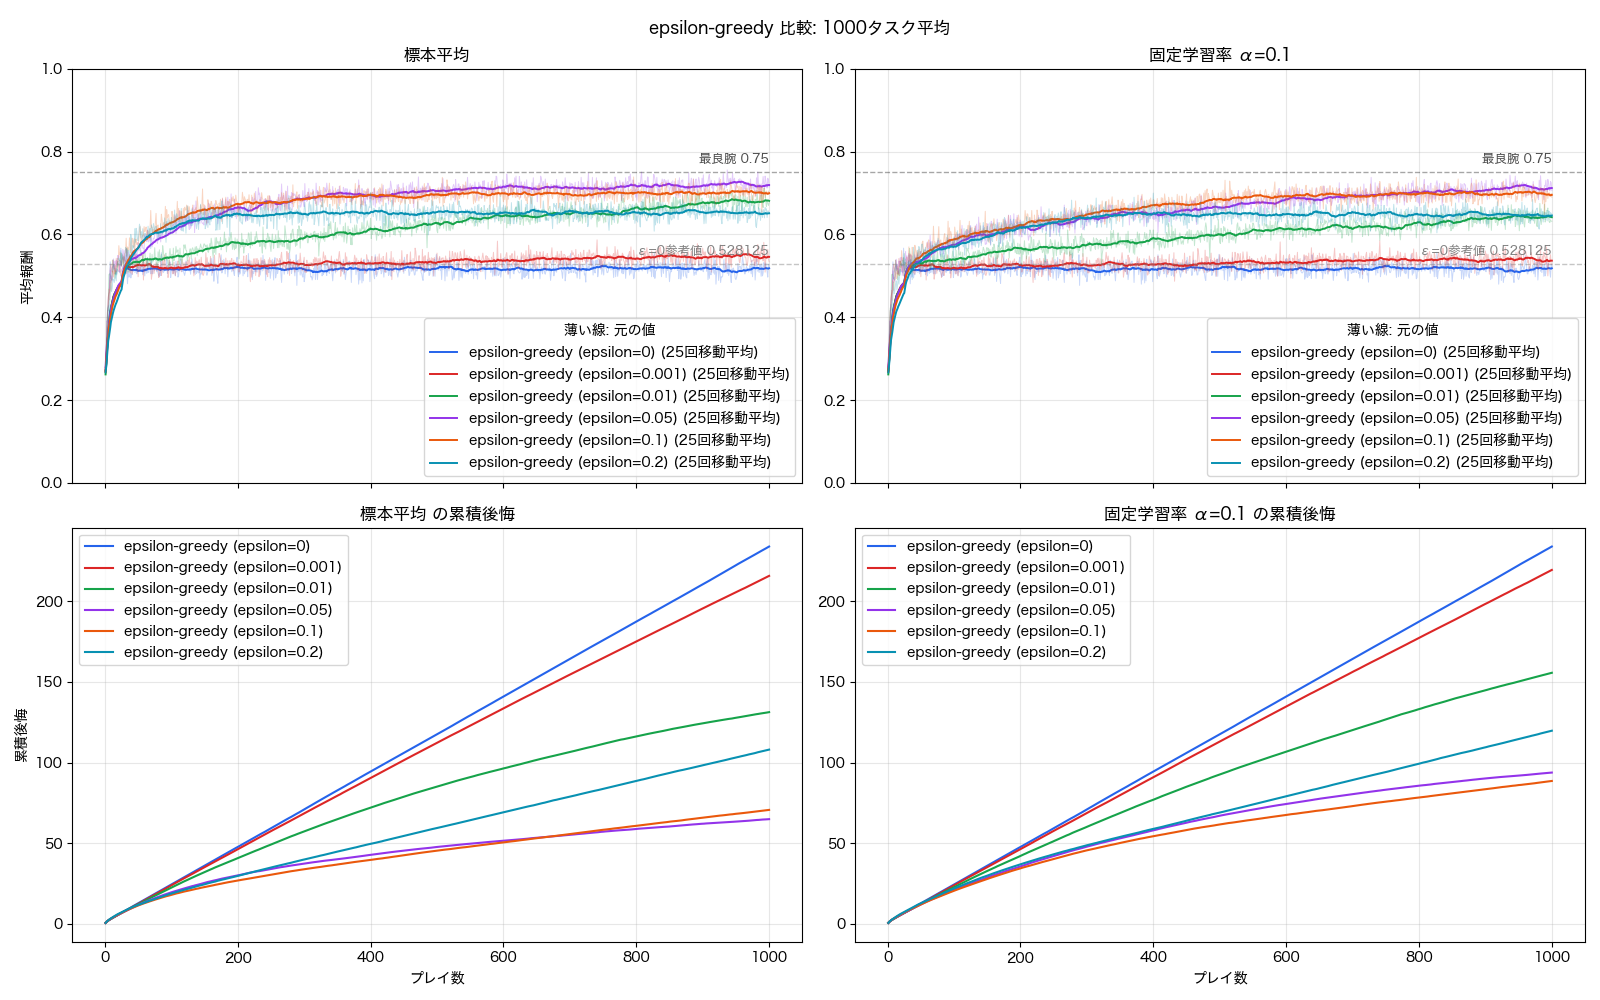
\includegraphics[width=\linewidth]{assets/reinforcement_column/greedy_graph.png}
  \captionof{figure}{greedy 法と $\varepsilon$-greedy 法の学習曲線}
  \label{fig:epsilon-greedy}
\end{center}

\ \textbf{greedy 法と $\varepsilon$-greedy 法}\\
図\ref{fig:epsilon-greedy}では，greedy 法と $\varepsilon$-greedy 法を比較した．
greedy 法は
\[
    A_t=\arg\max_{a\in\mathcal{A}}Q_t(a)
\]
により，常に現在の推定価値が最大の腕を選ぶ方法である．
一方，$\varepsilon$-greedy 法では，確率 $1-\varepsilon$ で greedy な腕を選び，
確率 $\varepsilon$ でランダムに腕を選ぶ．

\ $\varepsilon=0$ の greedy 法では，初期値をすべて $Q_0(a)=0$ とすると，
最初に報酬 $1$ を出した腕に固定されやすい．
報酬が出るまでは同点の腕をランダムに選ぶため，最初に成功する腕が $a$ である確率は
\[
    q_a=\frac{p_a}{\sum_{b=1}^{6}p_b}
\]
と近似できる．
したがって，長期的な平均報酬は
\[
    \bar{r}_{\infty}
    =
    \sum_{a=1}^{6}q_a p_a
    =
    \frac{\sum_{a=1}^{6}p_a^2}{\sum_{a=1}^{6}p_a}
\]
となる．
今回の設定では
\[
    \sum_{a=1}^{6}p_a=\frac{8}{5},
    \qquad
    \sum_{a=1}^{6}p_a^2=\frac{169}{200}
\]
であるから，
\[
    \bar{r}_{\infty}
    =
    \frac{169/200}{8/5}
    =
    \frac{169}{320}
    =
    0.528125
\]
となる．
これは図中の $\varepsilon=0$ の収束値とよく一致している．

\ 一方，$\varepsilon=0.2$ の場合，学習が十分進んで greedy 部分では第6腕を選べるようになったとしても，
全体の $20\%$ はランダムに腕を選ぶ．
このとき長期的な平均報酬はおよそ
\[
    (1-\varepsilon)p^\ast
    +
    \varepsilon \frac{1}{6}\sum_{a=1}^{6}p_a
\]
で与えられる．
今回の設定では $p^\ast=3/4$，
\[
    \frac{1}{6}\sum_{a=1}^{6}p_a
    =
    \frac{4}{15}
\]
であるから，
\[
    (1-0.2)\cdot\frac{3}{4}
    +
    0.2\cdot\frac{4}{15}
    \simeq
    0.653
\]
となる．
図で $\varepsilon=0.2$ の平均報酬が最適腕の $0.75$ より低い値に落ち着くのは，
学習後も一定確率で低報酬の腕を選び続けるためである．
つまり，\textbf{$\varepsilon$ は小さすぎても大きすぎてもよくない}．
今回の結果では，$\varepsilon=0.05$ から $0.1$ 程度が，
初期探索と後半の活用のバランスがよかった．

\ 累積後悔のグラフは，この違いを別の形で示している．
累積後悔の傾きは，各時刻でどれだけ報酬を取り逃しているか，すなわち瞬間的な後悔の大きさを表す．
たとえば，greedy 法が平均報酬 $\bar{r}_{\infty}$ の腕選択に固定されているとき，
累積後悔の傾きはおよそ
\[
    p^\ast-\bar{r}_{\infty}
\]
となる．
$\varepsilon=0$ では
\[
    \frac{3}{4}-0.528125=0.221875
\]
となり，後悔が大きな傾きで増え続ける．
これは，学習が速いというより，早い段階で誤った腕に固定されてしまっている状態である．

\ これに対して，$\varepsilon>0$ では初期に探索を行うため，序盤の累積後悔は増えやすい．
しかし，その探索によって最適腕を発見できれば，その後の累積後悔の傾きは小さくなる．
また，累積後悔の傾きが時間とともに小さく変化し続けている場合には，
腕の選択がまだ改善しており，学習が継続していると解釈できる．
逆に，累積後悔がほぼ直線になった場合には，腕の選択傾向がほぼ固定され，
その時点の方策で一定の損失を出し続けていると考えられる．
これは，初期に損をしてでも正しい腕を見つける「学習の速さ」と，
学習後に不要な探索をどれだけ減らせるかという「最終的な正確性」のトレードオフを表している．

\begin{center}
  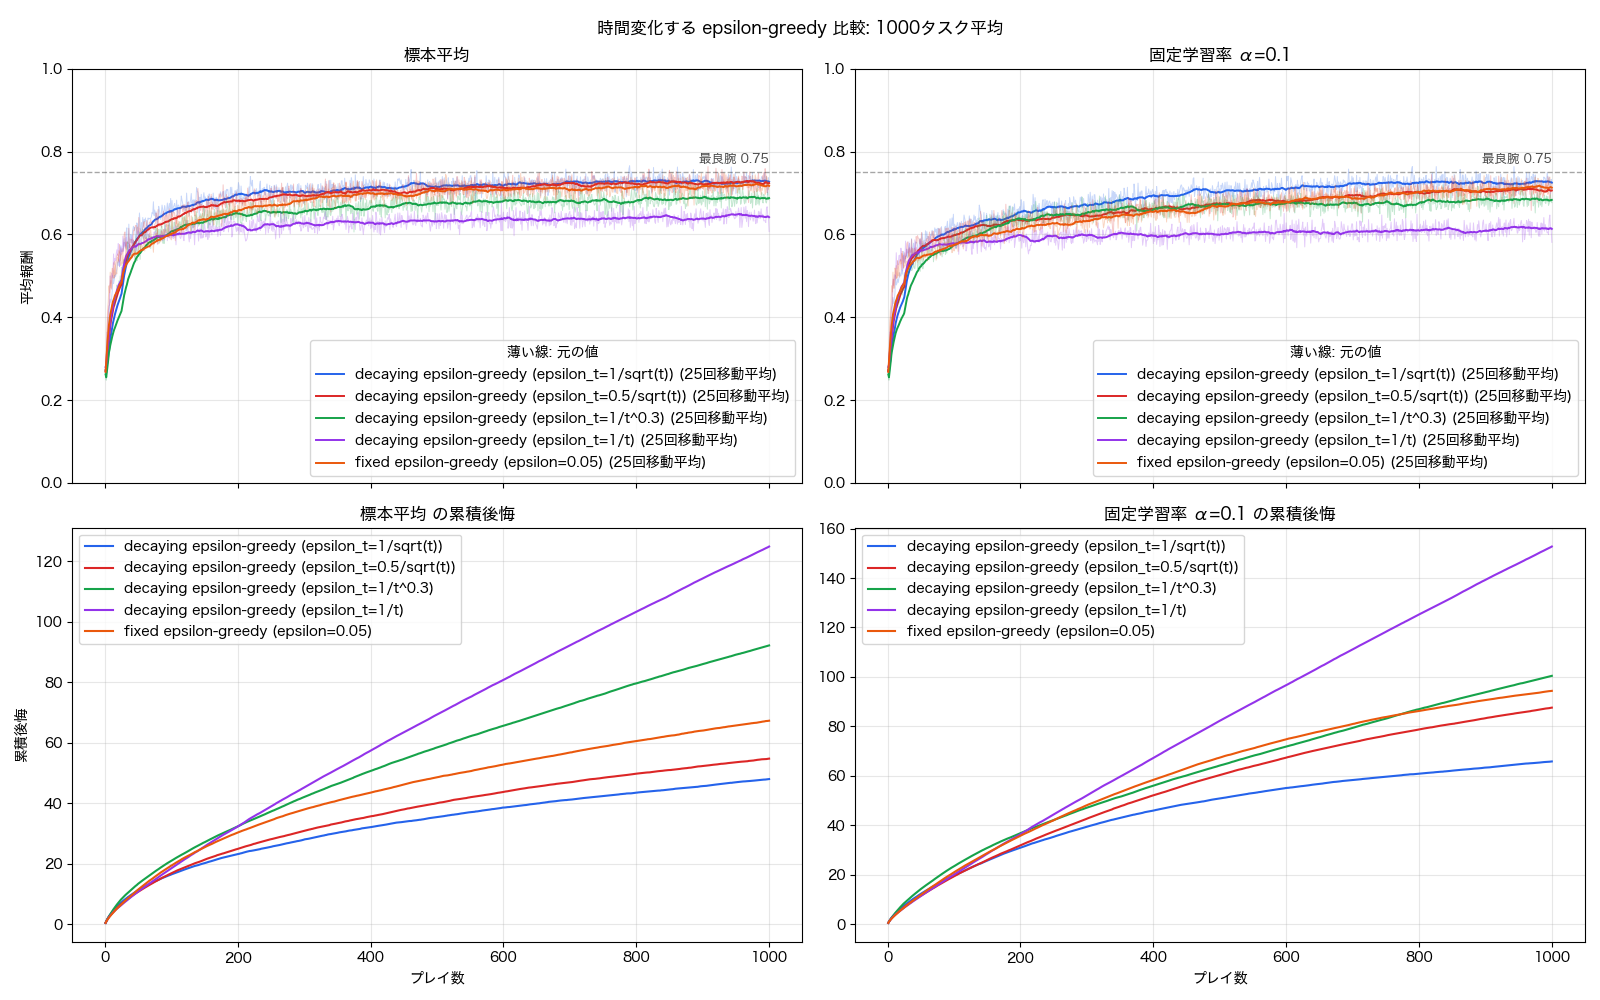
\includegraphics[width=\linewidth]{assets/reinforcement_column/time_greedy.png}
  \captionof{figure}{$\varepsilon$が時間変化する場合の学習曲線}
  \label{fig:decaying-epsilon-greedy}
\end{center}

\ \textbf{時間変化する $\varepsilon_t$-greedy 法}\\
固定した $\varepsilon$ を用いる $\varepsilon$-greedy 法では，
$\varepsilon$ が小さすぎると探索が不足し，初期に高く評価された腕に固定されやすい．
一方で，$\varepsilon$ が大きすぎると，最適腕を見つけた後もランダム探索が残り，
低報酬の腕を選ぶ損失が続いてしまう．
そこで，学習初期には十分に探索し，学習後半では不要な探索を減らすために，
時間とともに探索率を小さくする $\varepsilon_t$-greedy 法を考える．

\ $\varepsilon_t$-greedy 法では，
\[
    A_t =
    \begin{cases}
    \displaystyle \arg\max_{a\in\mathcal{A}} Q_t(a), & \text{確率 } 1-\varepsilon_t,\\
    \text{ランダムな腕}, & \text{確率 } \varepsilon_t
    \end{cases}
\]
として，各時刻 $t$ における探索率 $\varepsilon_t$ を変化させる．
本実験では，
\[
    \varepsilon_t=\frac{1}{\sqrt{t}},\quad
    \varepsilon_t=\frac{0.5}{\sqrt{t}},\quad
    \varepsilon_t=\frac{1}{t^{0.3}},\quad
    \varepsilon_t=\frac{1}{t}
\]
を比較し，固定値 $\varepsilon=0.05$ の場合とも比べた．

\ 図\ref{fig:decaying-epsilon-greedy}を見ると，
$\varepsilon_t=1/\sqrt{t}$ は，平均報酬と累積後悔の両方で比較的良い挙動を示している．
これは，時刻 $T$ までに発生するランダム探索の期待回数から説明できる．
$\varepsilon_t$-greedy 法では，各時刻に確率 $\varepsilon_t$ で探索を行うため，
探索回数 $M_T$ の期待値は
\[
    \mathbb{E}[M_T]
    =
    \sum_{t=1}^{T}\varepsilon_t
\]
である．
腕の本数を $K=6$ とすると，ランダム探索だけで各腕が試される回数の目安は
\[
    \frac{1}{K}\sum_{t=1}^{T}\varepsilon_t
\]
となる．

\ $\varepsilon_t=1/t$ の場合，
\[
    \sum_{t=1}^{T}\frac{1}{t}
    \simeq
    \log T
\]
である．
今回の実験では $T=1000$ なので，$\log 1000 \simeq 6.9$ となり，
各腕をランダム探索で試す回数は平均して1回程度にすぎない．
そのため，早い段階で探索率が小さくなりすぎ，
第6腕を十分に試す前に別の腕へ固定されやすい．

\ 一方，$\varepsilon_t=1/\sqrt{t}$ の場合，
\[
    \sum_{t=1}^{T}\frac{1}{\sqrt{t}}
    \simeq
    2\sqrt{T}
\]
である．
$T=1000$ では $2\sqrt{1000}\simeq 63$ となるため，
各腕はランダム探索だけでも平均して10回程度試される．
今回の報酬確率では，第6腕の報酬確率 $p_6=3/4$ と第5腕の報酬確率 $p_5=1/2$ の差が
\[
    \Delta=p_6-p_5=\frac{1}{4}
\]
と比較的大きい．
そのため，各腕を十数回程度試せば，第6腕が有望であることを発見するきっかけを得やすい．
さらに，$\varepsilon_t=1/\sqrt{t}$ は時間とともに $0$ に近づくため，
最適腕を見つけた後には不要なランダム探索が減り，平均報酬を高く保ちやすい．

\ これに対して，$\varepsilon_t=1/t^{0.3}$ の場合，
\[
    \sum_{t=1}^{T}\frac{1}{t^{0.3}}
    \simeq
    \frac{T^{0.7}}{0.7}
\]
であり，$T=1000$ ではおよそ $180$ 程度になる．
これは $\varepsilon_t=1/\sqrt{t}$ よりも探索回数が多く，
最適腕を発見するうえでは有利である．
しかし，学習後半にもランダム探索が多く残るため，
低報酬の腕を引く損失が続き，累積後悔の増加を抑えにくい．
つまり，$1/t$ は探索が減るのが速すぎ，$1/t^{0.3}$ は探索が残りすぎる．
その中間にある $1/\sqrt{t}$ は，今回の設定では
\textbf{探索不足と探索過多のバランス}がよかったと考えられる．

\ ここで，標本平均と固定学習率の違いにも注目したい．
固定した $\varepsilon$ の実験では両者の差は比較的小さかったが，
時間変化する $\varepsilon_t$ ではその差がより現れている．
標本平均手法では
\[
    Q_{t+1}(a)
    =
    Q_t(a)
    +
    \frac{1}{N_t(a)}\{r_t-Q_t(a)\}
\]
であり，腕 $a$ を多く選ぶほど新しい報酬の重み $1/N_t(a)$ は小さくなる．
一方，固定学習率では
\[
    Q_{t+1}(a)
    =
    Q_t(a)
    +
    \alpha\{r_t-Q_t(a)\}
\]
であり，新しい報酬は常に重み $\alpha$ で反映される．
実際，固定学習率の更新を展開すると
\[
    Q_n
    =
    (1-\alpha)^nQ_0
    +
    \sum_{i=1}^{n}\alpha(1-\alpha)^{n-i}r_i
\]
となり，最近の報酬ほど大きな重みを持つことが分かる．

\ 時間変化する $\varepsilon_t$ では，学習後半の探索機会が減るため，
後から得られた少数の観測をどれだけ強く価値推定に反映できるかが重要になる．
そのため，過去の観測を均等に平均する標本平均よりも，
最近の結果を大きく見る固定学習率の方が，減衰スケジュールの違いに敏感に反応しやすい．
このため，固定 $\varepsilon$ では目立たなかった価値更新方法の違いが，
時間変化する $\varepsilon_t$ の実験ではよりはっきり現れたと考えられる．

\ ただし，この結果は $\varepsilon_t=1/\sqrt{t}$ が一般に最適な減衰率であることを意味しない．
適切な減衰率は，腕の本数，プレイ回数，最適腕と次善腕の報酬確率差，
および価値更新方法に依存する．
今回の6本腕バンディット問題では，$T=1000$ という有限時間の中で，
$1/\sqrt{t}$ が「十分に探索するが，探索し続けすぎない」スケールになっていたと解釈できる．

\begin{center}
  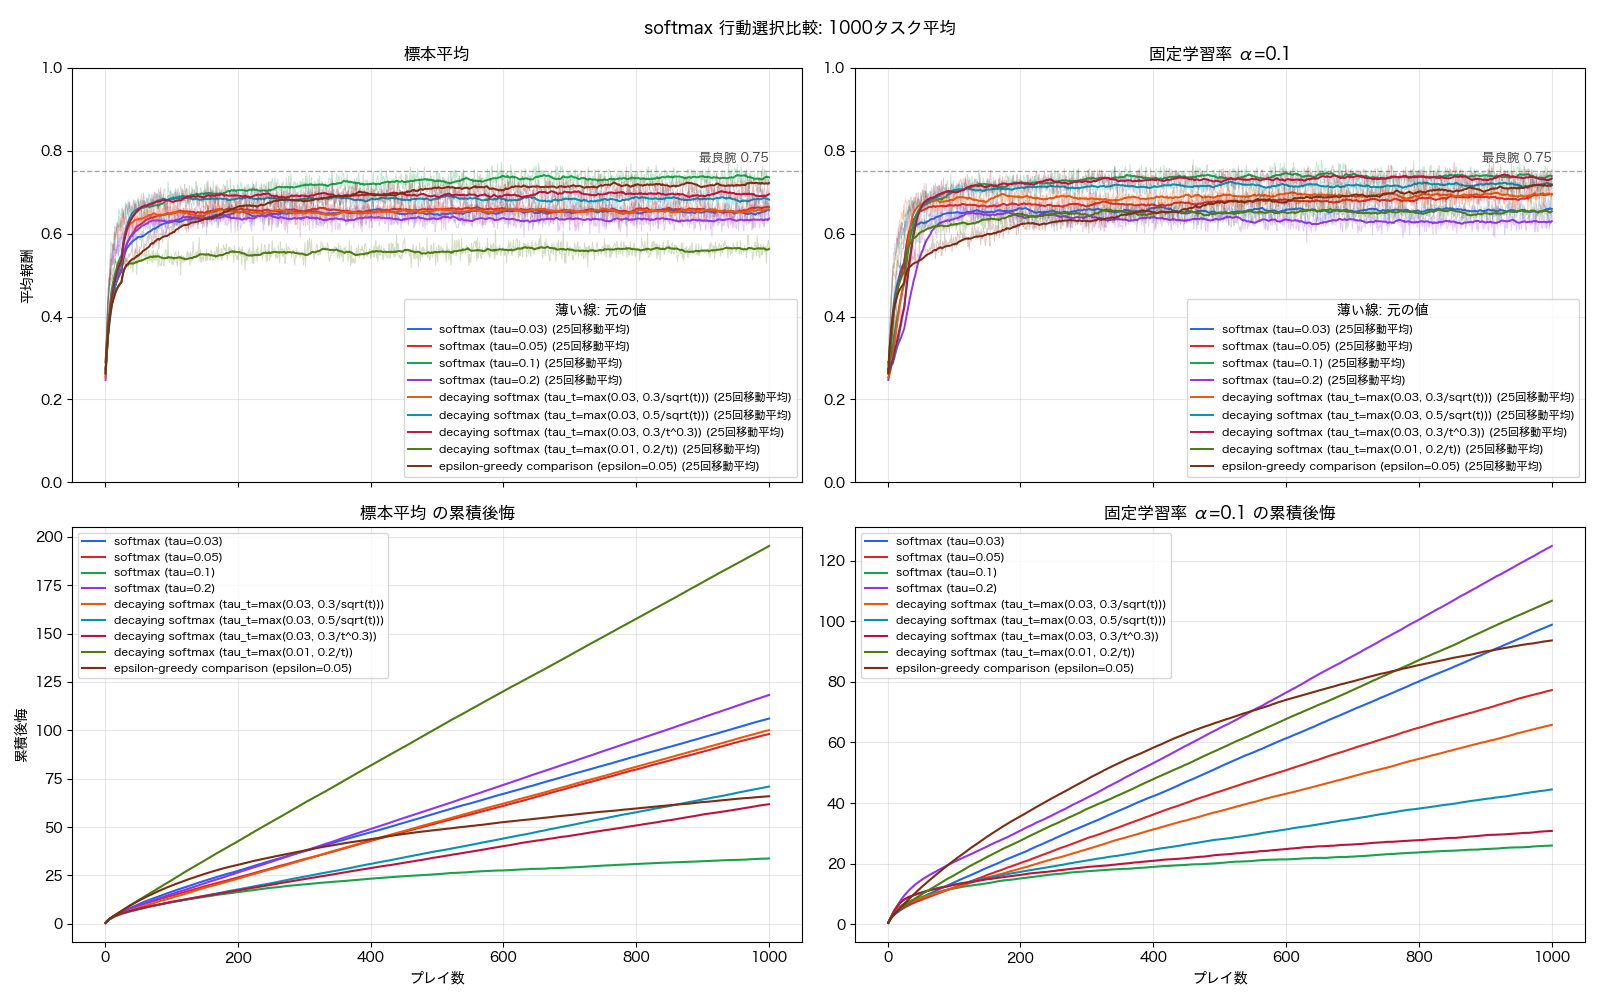
\includegraphics[width=\linewidth]{assets/reinforcement_column/softmax.png}
  \captionof{figure}{softmax 法の学習曲線}
  \label{fig:softmax}
\end{center}

\ \textbf{softmax 法}\\
次に，softmax による行動選択を比較する．
softmax 法では，各腕の推定行動価値 $Q_t(a)$ に対して
\[
    \Pr(A_t=a)
    =
    \frac{\exp(Q_t(a)/\tau)}
    {\sum_{b\in\mathcal{A}}\exp(Q_t(b)/\tau)}
\]
によって選択確率を与える．
ここで $\tau>0$ は温度パラメータであり，
$\tau$ が大きいほど各腕の選択確率は一様に近づき，
$\tau$ が小さいほど greedy 法に近づく．
したがって，$\tau$ は「価値の差をどれくらい鋭く行動選択に反映するか」を決める
スケールパラメータである．

\ 固定温度の結果を見ると，今回の設定では $\tau=0.1$ 付近が比較的よい性能を示している．
この理由は，今回の真の報酬確率の差の大きさから説明できる．
最適腕である第6腕と次善腕である第5腕の報酬確率差は
\[
    p_6-p_5
    =
    \frac{3}{4}-\frac{1}{2}
    =
    \frac{1}{4}
\]
である．
softmax では，2つの腕 $a,b$ の選択確率の比は
\[
    \frac{\Pr(A_t=a)}{\Pr(A_t=b)}
    =
    \exp\left(\frac{Q_t(a)-Q_t(b)}{\tau}\right)
\]
となる．
仮に推定値が真の報酬確率に近づき，
$Q_t(6)-Q_t(5)\simeq 0.25$ であるとすると，
$\tau=0.1$ のとき
\[
    \frac{\Pr(A_t=6)}{\Pr(A_t=5)}
    \simeq
    \exp\left(\frac{0.25}{0.1}\right)
    =
    \exp(2.5)
    \simeq 12.2
\]
となる．
つまり，第6腕は第5腕より十分選ばれやすいが，
第5腕が完全に排除されるほど極端でもない．
この程度の鋭さが，今回の問題では探索と活用のバランスとしてちょうどよかったと考えられる．

\ 一方，$\tau=0.2$ では
\[
    \exp\left(\frac{0.25}{0.2}\right)
    =
    \exp(1.25)
    \simeq 3.5
\]
となり，第6腕と第5腕の選択確率の差がそれほど大きくならない．
そのため，学習後も第5腕や他の腕を選ぶ確率が残りやすく，
平均報酬は最適値 $0.75$ から離れ，累積後悔も増えやすい．
逆に，$\tau=0.03$ のように温度が小さすぎると，
\[
    \exp\left(\frac{0.25}{0.03}\right)
    \simeq
    \exp(8.33)
\]
となり，わずかな価値差でも選択確率が極端に偏る．
学習が十分進んだ後であれば有利に働くが，
初期には $Q_t(a)$ の推定誤差が大きいため，
偶然高く評価された腕に選択が集中しやすい．

\ このように，softmax 法でも\textbf{温度は大きすぎても小さすぎてもよくない}．
今回の6本腕バンディット問題では，最適腕と次善腕の差が $0.25$ であるため，
$\tau=0.1$ 程度にすると
\[
    \frac{p_6-p_5}{\tau}
    =
    \frac{0.25}{0.1}
    =
    2.5
\]
となり，softmax の指数関数によって最適腕を十分に優遇しつつ，
完全な greedy にはならない程度の選択確率が得られる．
これが，固定温度 $\tau=0.1$ が今回うまく働いた主な理由である．

\ さらに，温度を時間とともに変化させる方法も試した．
これは，学習初期には温度を高めにして広く探索し，
学習が進むにつれて温度を下げることで，より価値の高い腕に選択を集中させる方法である．
本実験では，たとえば
\[
    \tau_t=\max\left(0.03,\frac{c}{\sqrt{t}}\right)
\]
のように，温度を減衰させつつ，下限値 $0.03$ を設けた．
下限を置いたのは，温度が小さくなりすぎるとほぼ greedy になり，
わずかな推定誤差にも過剰に反応してしまうためである．
図\ref{fig:softmax}では，温度を適切に減衰させた場合，
固定温度よりも累積後悔の増加を抑えられる場合がある．
これは，序盤では探索によって第6腕を発見する機会を確保し，
後半では温度低下によって第6腕への選択を強められるためである．

\begin{center}
  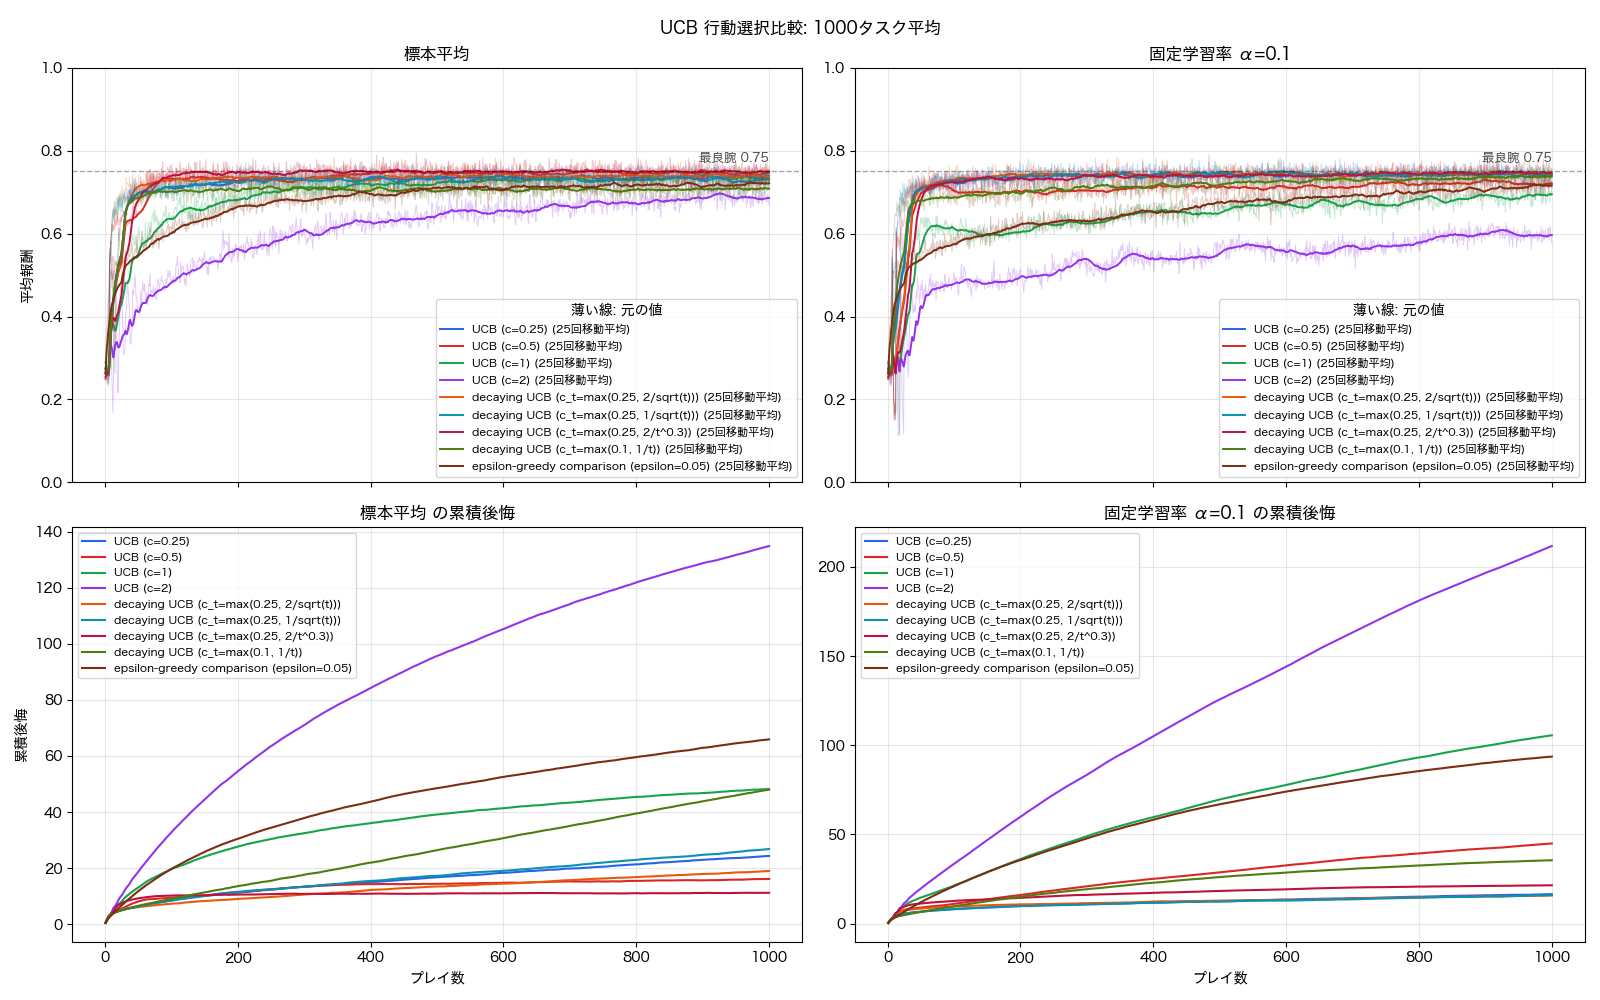
\includegraphics[width=\linewidth]{assets/reinforcement_column/ucb.png}
  \captionof{figure}{UCB 法の学習曲線}
  \label{fig:ucb}
\end{center}

\ \textbf{UCB 法}\\
次に，UCB による行動選択を比較する．
UCB は，現在の推定価値が高い腕だけでなく，
まだ十分に試されていない腕も高く評価する方法である．
具体的には，
\[
    A_t
    =
    \arg\max_{a\in\mathcal{A}}
    \left\{
        Q_t(a)
        +
        c\sqrt{\frac{\log t}{N_t(a)}}
    \right\}
\]
によって腕を選ぶ．
ここで $N_t(a)$ は時刻 $t$ までに腕 $a$ を選んだ回数であり，
$c>0$ は探索ボーナスの強さを決めるパラメータである．
第2項は，選択回数の少ない腕ほど大きくなるため，
UCB は単なるランダム探索ではなく，
\textbf{まだ不確実な腕を意図的に試す}方法と解釈できる．

\ 図\ref{fig:ucb}を見ると，$c$ が大きすぎる場合には性能が悪化している．
特に $c=2$ では平均報酬が低く，累積後悔も大きい．
これは，探索ボーナス
\[
    c\sqrt{\frac{\log t}{N_t(a)}}
\]
が大きすぎるために，すでに低報酬だと分かりつつある腕も繰り返し試してしまうからである．
今回の問題では，最適腕と次善腕の報酬確率差は
\[
    \Delta = p_6-p_5=\frac{1}{4}
\]
である．
したがって，探索ボーナスがこの差 $\Delta$ より十分大きい間は，
第6腕が高い推定価値を持っていても，試行回数の少ない腕が選ばれやすい．
つまり，$c$ が大きすぎると，UCB は慎重すぎる学習者になり，
不確実性を減らすための探索コストが累積後悔として残る．

\ 一方で，$c$ が小さい場合には，探索ボーナスが弱くなり，
現在の推定価値 $Q_t(a)$ をより重視する．
図では，$c=0.25$ や $c=0.5$ が比較的良い結果を示している．
これは，今回の6本腕バンディット問題では報酬確率の差が比較的大きく，
少ない試行回数でも第6腕の有利さを見つけやすかったためだと考えられる．

\ UCB の特徴は，累積後悔の傾きにも現れている．
$c$ が適切な場合，初期には全ての腕を試すために後悔が増えるが，
第6腕が有望であると分かるにつれて選択が集中し，
累積後悔の傾きが小さくなる．
一方，$c=2$ のように探索が強すぎる場合には，
後半になっても低報酬の腕を試す影響が残るため，
累積後悔の傾きが十分に小さくならない．

\ また，時間変化する UCB 係数 $c_t$ も比較した．
これは，学習初期には大きめの探索ボーナスで各腕を広く試し，
学習後半では探索ボーナスを小さくして，
推定価値の高い腕をより重視する方法である．
たとえば
\[
    c_t=\max\left(0.25,\frac{1}{\sqrt{t}}\right)
\]
のように設定すると，初期には強めに探索しつつ，
後半には $c_t$ が下限値 $0.25$ に近づく．
UCB の探索ボーナスそのものは
\[
    c_t\sqrt{\frac{\log t}{N_t(a)}}
\]
であるため，$c_t$ を小さくすることで後半の過剰な探索をさらに抑えられる．
ただし，$c_t$ を小さくしすぎると，
UCB の利点である「試行回数の少ない腕を体系的に試す」効果も弱くなる．
したがって，UCB でも探索の強さを問題のスケールに合わせることが重要である．

\begin{center}
  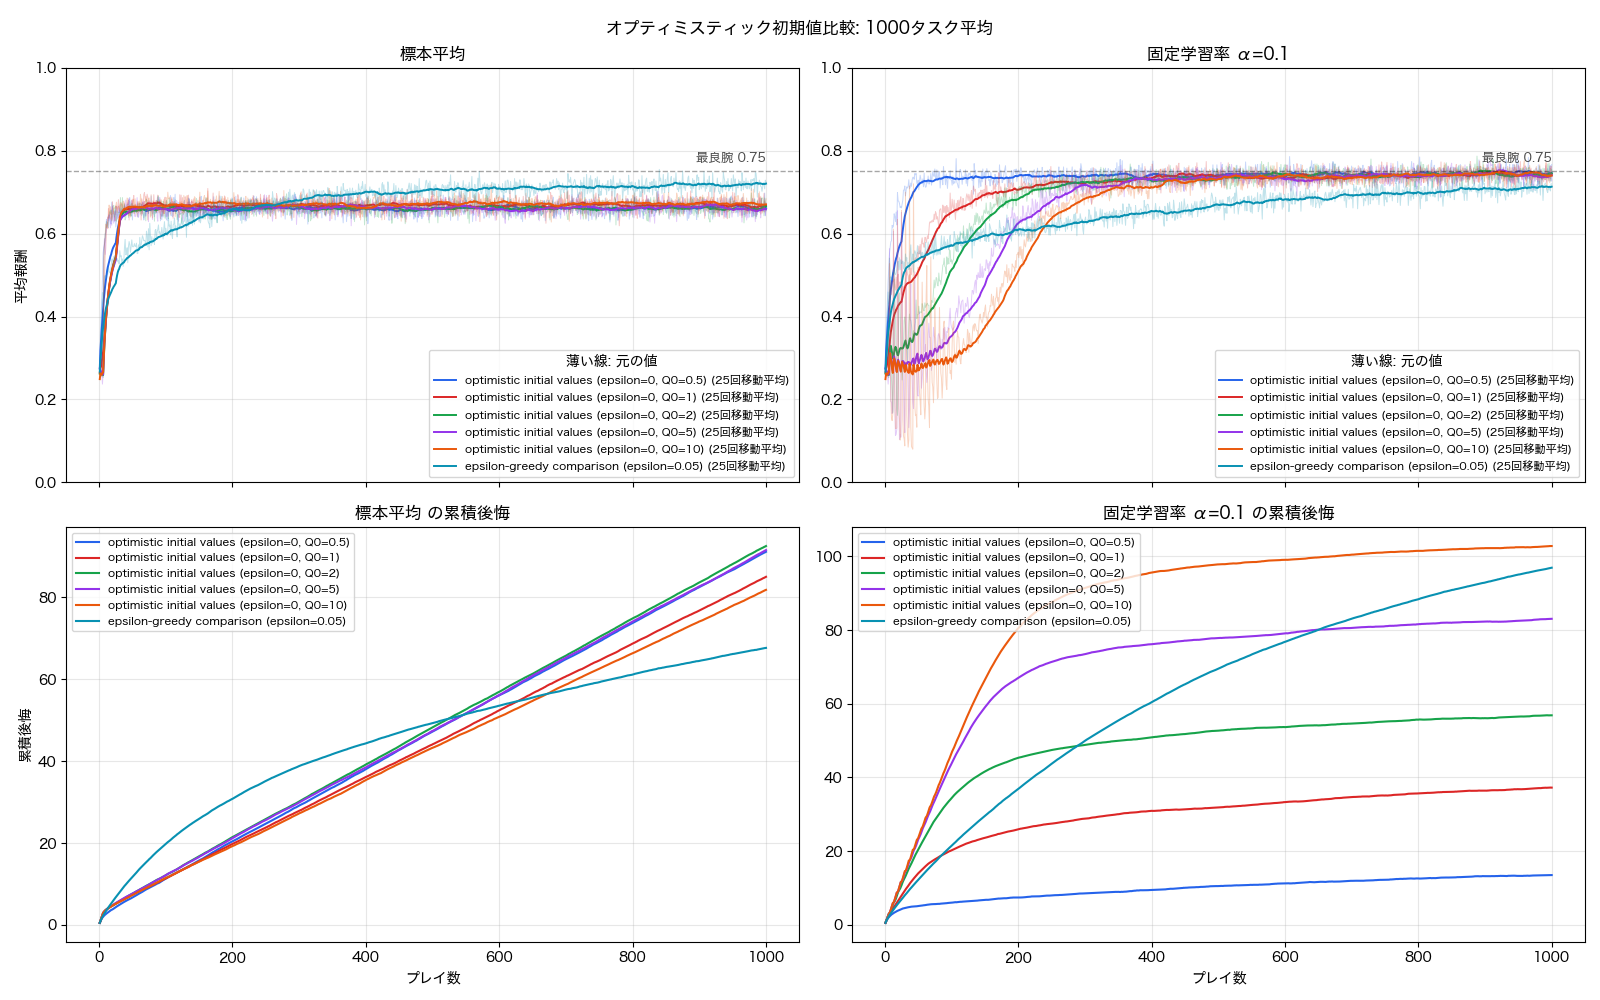
\includegraphics[width=\linewidth]{assets/reinforcement_column/optimistic.png}
  \captionof{figure}{オプティミスティック初期値の学習曲線}
  \label{fig:optimistic}
\end{center}

\ \textbf{optimistic 初期値}\\
次に，optimistic 初期値による探索を比較する．
これは，初期の行動価値 $Q_0(a)$ を高めに設定することで，
まだ十分に試していない腕を魅力的に見せる方法である．
本実験では $\varepsilon=0$ とし，明示的なランダム探索は行わず，
初期値の楽観性だけで探索がどの程度生じるかを調べた．

\ 図\ref{fig:optimistic}を見ると，標本平均を用いた場合には，
$Q_0$ を変えても最終的な結果はどれも似たように悪くなっている．
これは，標本平均手法では，腕 $a$ を初めて選んだ時点で
\[
    Q_1(a)=r_1
\]
となり，初期値 $Q_0(a)$ の影響がほとんど消えてしまうためである．
つまり，$Q_0$ をいくら大きくしても，その腕を一度試すと，
価値推定は実際に得られた $0$ または $1$ の報酬に置き換わる．
そのため，optimistic 初期値は「まだ一度も試していない腕を試させる」
効果は持つが，その後の価値推定には残りにくい．
結果として，標本平均では $Q_0$ の違いが学習曲線に大きく反映されず，
どの初期値でも似た挙動になったと考えられる．

\ 一方，固定学習率 $\alpha=0.1$ を用いた場合には，
初期値によって学習速度に大きな差が現れている．
固定学習率の更新は
\[
    Q_{n}(a)
    =
    (1-\alpha)^n Q_0(a)
    +
    \sum_{i=1}^{n}
    \alpha(1-\alpha)^{n-i}r_i
\]
と展開できる．
この式から分かるように，固定学習率では初期値の影響が
$(1-\alpha)^n Q_0(a)$ として残る．
したがって，$Q_0$ を大きくすると，その腕が何度か低い報酬を出しても，
しばらくは高く評価され続ける．

\ 図では，$Q_0=0.5$ の場合に平均報酬が早く高い値へ到達し，
累積後悔も小さくなっている．
これは，初期値が大きすぎず，初期の探索を促しつつ，
低報酬の腕への過大評価が比較的早く解消されたためだと考えられる．
逆に，$Q_0=5$ や $Q_0=10$ のように初期値が大きすぎると，
低報酬の腕も長い間高く評価され続ける．
たとえば報酬がしばらく $0$ だった場合，固定学習率では
\[
    Q_n(a)=(1-\alpha)^n Q_0(a)
\]
となる．
$\alpha=0.1$ では $(1-\alpha)^n=0.9^n$ なので，
$Q_0$ が大きいほど，その過大評価が十分に下がるまで多くの試行が必要になる．

\ 以上より，optimistic 初期値は，標本平均よりも固定学習率と組み合わせたときに
特徴が現れやすい．
標本平均では初期値が一度の観測でほぼ消えてしまうのに対し，
固定学習率では初期値の影響がしばらく残るため，
初期値の大きさが探索の強さと学習速度を大きく左右する．
ただし，初期値は大きければよいわけではなく，
小さすぎると探索を促せず，大きすぎると悪い腕への過大評価が長く残る．
今回の結果は，optimistic 初期値もまた，
問題の報酬スケールに合わせて設定する必要があることを示している．

\begin{center}
  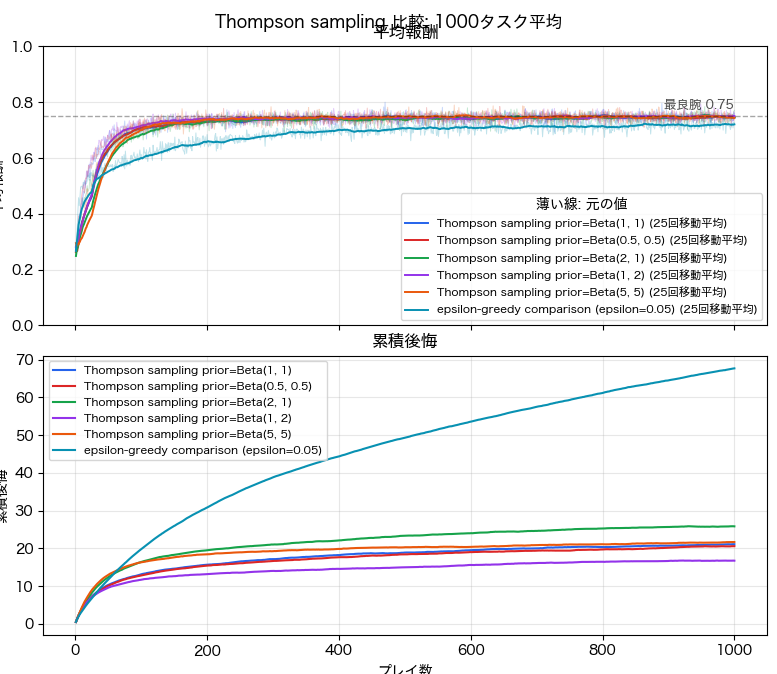
\includegraphics[width=\linewidth]{assets/reinforcement_column/thompson.png}
  \captionof{figure}{Thompson sampling の学習曲線}
  \label{fig:thompson}
\end{center}

\ \textbf{Thompson sampling}\\
最後に，Thompson sampling による行動選択を比較する．
Thompson sampling では，各腕の報酬確率そのものを一点推定するのではなく，
その不確実性を確率分布として保持する．
各時刻では，腕 $a$ の報酬確率に関する事後分布から値をサンプリングし，
そのサンプル値が最大となる腕を選ぶ．

\ 今回の実験では報酬が Bernoulli$(p_a)$ に従うため，
各腕の成功確率 $p_a$ に対してベータ分布を用いる．
時刻 $t$ における腕 $a$ の事後分布を
\[
    p_a \sim \mathrm{Beta}(\alpha_a,\beta_a)
\]
とし，そこから
\[
    \tilde{p}_a \sim \mathrm{Beta}(\alpha_a,\beta_a)
\]
をサンプリングして，
\[
    A_t=\arg\max_{a\in\mathcal{A}}\tilde{p}_a
\]
により腕を選ぶ．
報酬 $1$ が得られた場合は $\alpha_a$ を増やし，
報酬 $0$ が得られた場合は $\beta_a$ を増やす．
したがって，Thompson sampling では，探索は外から加えるランダム行動ではなく，
\textbf{報酬確率に関する不確実性}から自然に生じる．

\ 図\ref{fig:thompson}では，事前分布の違いによる学習曲線の変化を比較している．
ベータ分布 $\mathrm{Beta}(\alpha,\beta)$ の平均は
\[
    \mathbb{E}[p]
    =
    \frac{\alpha}{\alpha+\beta}
\]
であり，$\alpha+\beta$ が大きいほど事前分布は強くなる．
つまり，$(\alpha,\beta)$ は単なる初期値ではなく，
「はじめにどの程度の成功・失敗を仮想的に見たことにするか」を表している．

\ 結果を見ると，Thompson sampling は全体として
$\varepsilon$-greedy の比較対象よりも累積後悔が小さく，
平均報酬も早く高い値に近づいている．
これは，各腕の不確実性を分布として持つことで，
まだ情報が少ない腕には自然に探索の余地が残り，
成功が多く観測された腕には選択が集まりやすくなるためである．

\ 事前分布の違いに注目すると，
$\mathrm{Beta}(1,2)$ が特に小さい累積後悔を示している．
この事前分布の平均は $1/3$ であり，成功確率をやや低めに見積もる悲観的な事前分布である．
今回の問題では低報酬の腕が多いため，成功確率をやや低く見る事前分布は，
低報酬の腕を早めに見切る方向に働きやすい．
その一方で，第6腕のように成功が多く観測される腕では，
事後分布がすぐに高い値へ移動するため，選択が集中しやすい．

\ 一方，$\mathrm{Beta}(2,1)$ は平均 $2/3$ を持つ楽観的な事前分布である．
この場合，各腕の成功確率を初期には高めに見積もるため，
低報酬の腕についても「本当は良い腕かもしれない」という不確実性が残りやすい．
その結果，低報酬の腕を見切るまでにやや時間がかかり，
累積後悔が大きくなりやすい．
これは，optimistic 初期値において初期値を大きくしすぎると
悪い腕への過大評価が長く残ることと似ている．

\ また，$\mathrm{Beta}(0.5,0.5)$ は U 字型の分布であり，
成功確率が $0$ 付近または $1$ 付近にある可能性を比較的大きく見る事前分布である．
そのため，初期にはサンプル値が極端になりやすく，
不確実性に基づく探索がやや強く出る．
一方，$\mathrm{Beta}(5,5)$ は平均 $1/2$ の周辺に集中した事前分布であり，
初期にはどの腕も中程度の成功確率を持つという強めの信念を置く．
この場合，観測が少ない段階では事前分布の影響が残り，
第6腕の優位性を反映するまでに少し時間がかかる．

\ この結果から，Thompson sampling における事前分布は，
単なる初期設定ではなく，探索の性質そのものを決める要素であることが分かる．
中立的な事前分布では観測に素直に反応し，
楽観的な事前分布では探索が長く残りやすく，
悲観的な事前分布では低報酬の腕を早く見切りやすい．
ただし，悲観的すぎる事前分布では本当に良い腕を十分に試す前に
候補から外してしまう危険もあるため，事前分布も問題の報酬スケールに依存して調整される．

\begin{center}
  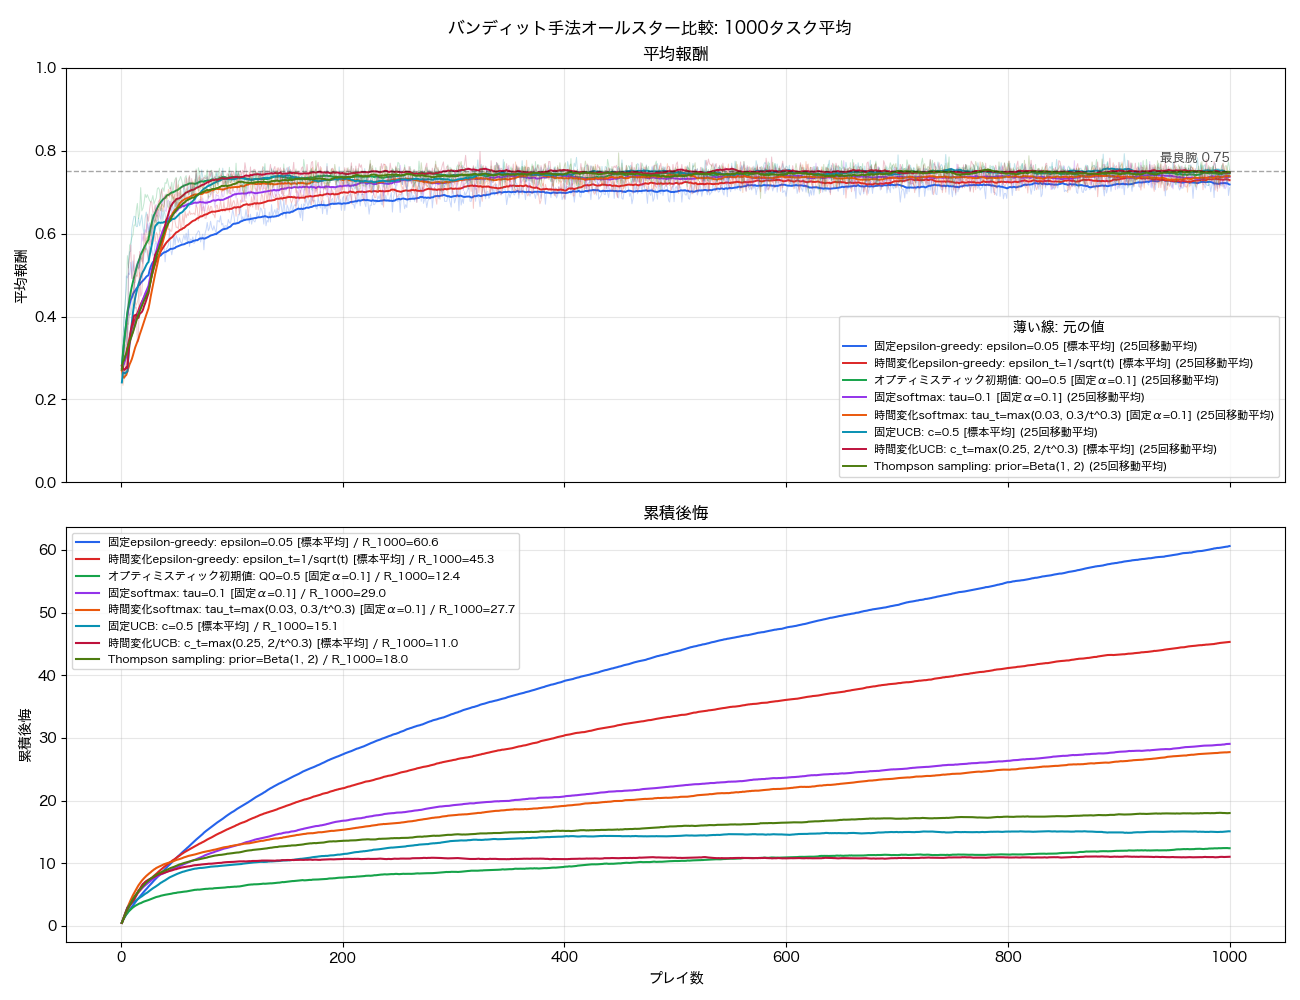
\includegraphics[width=\linewidth]{assets/reinforcement_column/allstar.png}
  \captionof{figure}{全手法の，最も累積後悔が小さくなるようなパラメータでの学習曲線}
  \label{fig:bandit-allstar}
\end{center}

\ \textbf{手法間の比較とまとめ}\\
最後に，各手法について今回の問題で比較的よい性能を示したパラメータを選び，
同一の図で比較した．
図\ref{fig:bandit-allstar}を見ると，平均報酬の推移だけでは，
多くの手法が最終的に最適腕の期待報酬 $0.75$ 付近へ近づいており，
大きな差は見えにくい．
しかし，累積後悔を見ると，各手法の違いはかなり明確に現れる．
これは，平均報酬が「最終的にどこまで到達したか」を見る指標であるのに対し，
累積後悔は「そこに至るまでにどれだけ損をしたか」を記録する指標だからである．

\ 今回の結果では，optimistic 初期値，時間変化する UCB，固定 UCB が特に小さい累積後悔を示している．
optimistic 初期値は，初期価値を高く設定することで未試行の腕を自然に試させるため，
初期の探索を素早く行うことができる．
今回のように定常的で，かつ最適腕と次善腕の差が比較的大きい問題では，
一度よい腕を見つければそのまま活用しやすく，累積後悔が小さくなったと考えられる．
また UCB は，試行回数の少ない腕に探索ボーナスを与えるため，
ランダムに探索するのではなく，不確実な腕を体系的に試すことができる．
その結果，探索の無駄が少なく，早い段階で第6腕へ選択を集中できたと解釈できる．

\ 一方で，固定 $\varepsilon$-greedy は累積後悔が大きくなっている．
これは，最適腕を見つけた後も確率 $\varepsilon$ でランダム探索を続けるためである．
学習が十分に進んだ後の平均報酬は
\[
    (1-\varepsilon)p^\ast
    +
    \varepsilon \frac{1}{K}\sum_{a=1}^{K}p_a
\]
で近似されるため，$\varepsilon>0$ である限り，
低報酬の腕を引く損失が残る．
時間変化する $\varepsilon_t$-greedy は，初期には探索し，
後半には $\varepsilon_t$ を小さくすることでこの問題を緩和している．

\ softmax でも，固定温度では学習後も確率的な選択が残る．
温度 $\tau$ が大きいと探索が残りすぎ，温度が小さいと初期の推定誤差に過敏になる．
今回の比較では，時間変化する softmax は固定 softmax よりよい結果を示しており，
温度を下げながら探索から活用へ移行することの有効性が見られる．
ただし，softmax は価値差を指数関数で選択確率に変換するため，
適切な温度スケールは報酬確率差に強く依存する．
今回うまくいった温度が，他の報酬スケールでもそのまま有効とは限らない．

\ Thompson sampling も比較的良い結果を示している．
探索率や温度を外から指定するのではなく，
各腕の報酬確率に関する事後分布からサンプリングすることで探索が生じるため，
明示的な探索率を設定しなくても，探索と活用のバランスを比較的うまく取ることができたと考えられる．

\ ただし，ここまでの結果は\textbf{定常バンディット問題}における比較である．
各腕の真の報酬確率 $p_a$ が時刻によらず一定であるという仮定のもとでは，
過去の観測を蓄積することに意味があり，
標本平均，UCB，Thompson sampling のように，
観測回数が増えるほど推定を確信していく手法が有効に働きやすい．
しかし，非定常環境では古い観測が現在の環境を表さない可能性がある．
そのため，過去の全データを同じ重みで用いる標本平均手法は，
変化後の最適腕に追従しにくい．

\ この観点から見ると，定常環境で特に意味を持つ手法と，
非定常環境でも活かしやすい手法を分けて考える必要がある．
標本平均に基づく greedy，UCB，通常の Thompson sampling は，
基本的には「真の報酬確率が一定であり，観測を重ねるほど正しい値に近づく」
という考え方に支えられている．
したがって，定常環境では強いが，非定常環境では古い情報を信じすぎる危険がある．
特に UCB では，ある腕を十分に試した後は探索ボーナス
\[
    c\sqrt{\frac{\log t}{N_t(a)}}
\]
が小さくなるため，環境変化後にその腕を再び探索する力は弱くなる．
Thompson sampling でも，観測数が増えて事後分布が鋭くなると，
過去の信念が強く残り，新しい変化に反応しにくくなる場合がある．

\ 一方，固定学習率による価値更新や，探索率・温度・UCB係数を時間変化させる設計は，
非定常環境へ拡張する余地を持つ．
固定学習率では
\[
    Q_n
    =
    (1-\alpha)^nQ_0
    +
    \sum_{i=1}^{n}\alpha(1-\alpha)^{n-i}r_i
\]
となり，最近の報酬ほど大きな重みを持つ．
したがって，古い観測を徐々に忘れながら，新しい環境に追従しやすい．
同様に，非定常環境では探索率を完全には下げきらず，
一定の探索を残すことにも意味がある．
定常環境では不要な探索は後悔を増やすが，
非定常環境では，環境変化を発見するための観測機会になるからである．

\ 以上の比較から，多腕バンディット問題における手法の良し悪しは，
単に平均報酬の高さだけでは判断できないことが分かる．
それぞれの違いは，最適腕をどれだけ早く見つけるか，
低報酬の腕をどれだけ早く見切るか，
そして学習後に不要な探索をどれだけ残すかという形で，
累積後悔の曲線に現れる．

\ 本実験を通じて，多腕バンディット問題は，
強化学習における探索と活用を理解するための最小構成の実験場であることが確認できた．
状態遷移を持たない単純な問題であっても，
探索率，温度，探索ボーナス，初期値，事前分布，学習率の選び方によって，
学習曲線は大きく変化する．
したがって，より複雑な強化学習問題を扱う際にも，
アルゴリズムを名前で選ぶのではなく，
その手法が\textbf{何を不確実とみなし，どのように探索し，どの程度過去を信じるのか}
を考えることが重要である．

\end{column}
\clearpage

\input{chapters/machine_learning/generative_model.tex}
\clearpage
\begin{column}{Persona駆動型LLMによる災害後居住地選択モデル}{三木隆斗}
本章では，生成モデルを「観測データの背後にある構造を仮定し，その構造から観測が生じる」と捉えた．この考え方は，画像や文章の生成だけでなく，人間の選択行動のモデル化にも応用できる．ここでは，津波避難後の居住地選択を，personaを潜在表現として用いるLLMモデルで記述した例を紹介する．焦点は，LLMを単に分類器として使うのではなく，世帯ごとの見えにくい選好や判断基準をpersonaとして表現し，それをloading関数で選択する点にある．

\medskip
\noindent
\textbf{研究背景}

戦争，紛争，巨大災害の後には，被災者の避難，移住，再定住といった長期的な人口移動が発生する．とくに人口減少傾向にある地域では，災害後に誰がどこへ移るかが，その後の地域の人口構成，復興事業の進み方，公共住宅の需要，生活圏の再編に大きく影響する．したがって，災害後の居住地選択を理解することは，復興計画や住宅供給のマネジメントにとって重要である．

一方で，この現象は通常の交通行動モデルより扱いにくい．既存の交通計画理論では，通勤や買物，避難時の移動のように，比較的短期の選択を扱うことが多い．しかし，災害後の移住や定住は数年から数十年単位で進む長期現象であり，次のような難しさがある．

\begin{itemize}
\item 長期的な定量データを得にくい．
\item 世帯ごとの居住履歴が不完全になりやすい．
\item 復興制度，住宅供給，地域条件，家族事情が絡み合う．
\item 観測属性だけでは，帰還意向や再建意欲などの判断基準を捉えにくい．
\end{itemize}

このような背景から，表形式の変数だけでなく，世帯の履歴や地域文脈を文章として扱えるモデルが必要になる．大規模言語モデル（large language model; LLM）は，人間の判断過程を文脈依存的に表現しうるため，従来の離散選択モデルでは表しにくい半構造的な意思決定文脈を入力できる．

\medskip
\noindent
\textbf{使用データ}

使用したデータは，2026年3月に実施された被災者アンケートである．対象は，災害時の居住地域が宮城県・岩手県・福島県のいずれかであった世帯であり，個人属性，世帯属性，居住地選択履歴，住宅類型などの情報を含む．データの規模は次の通りである．

\begin{center}
\scriptsize
\begin{tabular}{lr}
\toprule
項目 & 件数 \\
\midrule
世帯数 & 5,002 \\
各世帯の状態数 & 11,662 \\
居住地移動サンプル数 & 6,660 \\
\bottomrule
\end{tabular}
\end{center}

学習・評価の分割は世帯単位で行った．これは，同一世帯の履歴が訓練データとテストデータにまたがると，履歴情報を通じた情報漏洩が起こりうるためである．LLMによる評価は計算コストが大きいため，テストデータのうち先頭200件を用いた．

\begin{center}
\scriptsize
\begin{tabular}{lrr}
\toprule
分割 & 移動サンプル数 & 世帯サンプル数 \\
\midrule
訓練データ & 4,691 & 3,542 \\
バリデーション & 982 & 709 \\
テスト & 987 & 751 \\
LLM評価 & 200 & 151 \\
\bottomrule
\end{tabular}
\end{center}

\medskip
\noindent
\textbf{予測タスク}

予測タスクは，各世帯の時点 \(t\) までの情報から，次時点 \(t+1\) の居住状態変化を予測する問題である．
\begin{equation}
x_{i,t}=\phi(s_{i,0:t}), \qquad
y_{i,t}=g(s_{i,t},s_{i,t+1}) \in \mathcal{Y}.
\end{equation}
ここで \(x_{i,t}\) は世帯 \(i\) について時点 \(t\) までに観測可能な属性・履歴から作る特徴量，\(s_{i,t}\) は地域，住宅類型，復興段階，時点などを含む居住状態，\(y_{i,t}\) は次状態への遷移を分類したラベルである．将来情報など，予測時点 \(t\) で本来分からない情報は入力から除外した．符号化前の推論時特徴量数は31である．

選択肢集合 \(\mathcal{Y}\) は次の6種類である．

\begin{center}
\scriptsize
\begin{tabular}{lrr}
\toprule
選択肢 & サンプル数 & 比率 \\
\midrule
現在地にとどまる & 519 & 7.8\% \\
被災地域内の仮住まいへ移る & 241 & 3.6\% \\
被災地域外の仮住まいへ移る & 1,676 & 25.2\% \\
災害公営住宅に移る & 340 & 5.1\% \\
自力再建先に移る & 3,286 & 49.3\% \\
帰還する & 598 & 9.0\% \\
\bottomrule
\end{tabular}
\end{center}

この分布から分かるように，「自力再建先に移る」がほぼ半数を占める．したがって，単純に多数派を選ぶモデルでも一定の正解率は出るが，少数クラスを識別できるか，また全体の移動分布を再現できるかが重要になる．

\medskip
\noindent
\textbf{LLMを使う動機}

多項ロジットモデルやニューラルネットワークは，表形式に整理された特徴量を入力として扱う．これに対して，災害後の居住地選択では，「なぜ帰還できないのか」「なぜ仮住まいを継続するのか」「自力再建を選ぶ条件は何か」といった説明的な文脈が重要である．これらは，単純な数値変数だけでは表しきれない．

そこで，LLMへのプロンプトには，世帯属性，居住履歴の文章要約，災害後の地域文脈，仮住まい・帰還・自力再建などの候補説明を含める．さらに，その世帯がどのような判断傾向を持ちそうかを表すpersonaを与える．LLMは，これらの文脈を読んだ上で，6つの選択肢の中から次の居住地選択を出力する．

\medskip
\noindent
\textbf{personaを潜在変数として見る}

personaとは，個票データから直接観測される変数ではなく，世帯の行動傾向や判断基準を文章で要約した潜在表現である．たとえば，同じ「仮住まい中」という状態でも，早期帰還を望む世帯，自力再建を目指す世帯，災害公営住宅を待つ世帯では，次の選択が異なる可能性がある．この差は，年齢や世帯人数のような観測属性だけでなく，生活再建の方針や地域へのこだわりによっても生じる．

生成モデルの記法でいえば，観測された特徴量 \(x\) と選択 \(y\) の背後に，直接観測されないpersona \(m\) があるとみなせる．
\begin{equation}
p(y\mid x)
=
\sum_m p(y\mid x,m)\,p(m\mid x).
\end{equation}
ここで \(p(m\mid x)\) は対象世帯にどのpersonaを割り当てるかを表すloadingであり，\(p(y\mid x,m)\) は，そのpersonaを文脈として与えたLLMが各選択肢を選ぶ分布に対応する．これは，潜在変数モデル
\begin{equation}
p_\theta(x)=\int p_\theta(x\mid z)p(z)\,dz
\end{equation}
において，観測されない \(z\) を周辺化する考え方と対応している．本研究では，personaがこの \(z\) に相当する役割を持つ．

\medskip
\noindent
\textbf{persona bankを用いた推論の流れ}

personaを使った推論は，次の手順で行う．

\begin{enumerate}
\item 訓練データの世帯属性・居住履歴をLLMに与え，世帯の行動傾向を説明するpersonaを作成する．
\item 作成したpersonaをpersona bankとして保存する．
\item 予測対象世帯の属性・履歴から，近いpersonaをloading関数で選ぶ．
\item 現在状態，居住履歴，選択肢説明，選ばれたpersonaをLLMへのプロンプトに入れる．
\item LLMが6つの候補から次の居住地選択を出力する．
\end{enumerate}

重要なのは，personaそのものが最終予測ではない点である．personaは，LLMが文脈依存的な判断を行うための補助的な潜在表現である．したがって，同じpersonaが選ばれても，現在地，履歴，選択肢説明が異なれば，異なるchoiceが出ることが望ましい．

\medskip
\noindent
\textbf{コサイン類似度によるloading}

もっとも単純なloadingは，予測対象世帯とpersona bank内の各personaをベクトル化し，類似度が最大のpersonaを選ぶ方法である．世帯属性や履歴要約をベクトル化する関数を \(\psi(\cdot)\)，persona \(m\) の表現を \(p_m\) とすると，
\begin{equation}
m^*(x)
=
\argmax_m
\operatorname{sim}\{\psi(x),\psi(p_m)\}
\end{equation}
と書ける．コサイン類似度を使う場合，
\begin{equation}
\operatorname{sim}\{\psi(x),\psi(p_m)\}
=
\frac{\psi(x)^\top \psi(p_m)}
{\|\psi(x)\|\|\psi(p_m)\|}
\end{equation}
である．

この方法は直感的で実装しやすい．しかし，属性や履歴が近いpersonaが，選択行動の予測に最も有効とは限らない．たとえば，年齢や家族構成は似ていても，住宅再建への意向や元居住地へのこだわりが異なれば，次の居住地選択は変わりうる．したがって，単純な類似度だけでは，choiceに効くpersonaを選びきれない可能性がある．

\medskip
\noindent
\textbf{EMアルゴリズム的なlearned loading}

そこで，persona割当そのものを観測されない潜在変数の推論問題とみなし，loading関数を学習する．真の「この世帯にはどのpersonaが対応するか」はデータに含まれていない．一方で，各世帯が実際にどの居住地選択をしたかは観測されている．したがって，personaの割当を，観測されたchoiceをよく説明するように更新することが考えられる．

この発想は，EMアルゴリズムに似ている．EMでは，観測されない潜在変数 \(z\) の事後分布をE-stepで推定し，その推定結果を使ってM-stepでモデルパラメータを更新する．ここでは，persona \(m\) が潜在変数に相当し，loading関数が \(p_\alpha(m\mid x)\) を与えると考える．\(\alpha\) はloading関数のパラメータである．

まず，現在のloading関数に基づいて，世帯 \(i\) がpersona \(m\) に対応する重みを計算する．
\begin{equation}
r_{im}
=
p_\alpha(m\mid x_i)
=
\frac{\exp\{\operatorname{sim}_\alpha(x_i,p_m)\}}
{\sum_{m'}\exp\{\operatorname{sim}_\alpha(x_i,p_{m'})\}}.
\end{equation}
これは，各personaに対するsoft assignmentであり，GMMのEMにおける責務 \(\gamma_{nk}\) と似た役割を持つ．これがE-step的な部分である．

次に，LLMまたは選択モデルが，persona \(m\) を与えたときに観測choice \(y_i\) をどれだけ説明できるかを評価する．理想的には，
\begin{equation}
\sum_i \sum_m r_{im}\log p_\theta(y_i\mid x_i,m)
\end{equation}
が大きくなるように，loading関数のパラメータ \(\alpha\) を更新する．これがM-step的な部分である．実装上は，LLMの内部パラメータを直接更新するのではなく，どのpersonaを選ぶと観測choiceへの適合が高くなるかを用いて，類似度関数 \(\operatorname{sim}_\alpha(\cdot,\cdot)\) を調整する．

このlearned loadingは，単に「属性が近いpersona」を選ぶのではなく，「choiceの予測に効くpersona」を選ぼうとする点に特徴がある．生成モデルの言葉でいえば，personaの事後分布 \(p(m\mid x,y)\) を完全には計算できないため，観測choiceを手がかりに近似的にloadingを改善していると解釈できる．

\medskip
\noindent
\textbf{評価指標と比較モデル}

評価には，個票単位の正解率だけでなく，少数クラスや移動分布の再現性を見る指標を用いた．Accuracyは直感的だが，多数派クラスに引っ張られやすい．Macro F1は各選択肢を同じ重みで評価するため，少数クラスを拾えているかを見やすい．また，Share MAEとJSDは，観測された選択肢シェアと予測シェアのずれを見る指標であり，人口移動分布の再現性を評価するために用いた．

\begin{align}
\mathrm{Acc}
&=
\frac{1}{N}\sum_i \mathbf{1}(\hat{y}_i=y_i),\\
\mathrm{MacroF1}
&=
\frac{1}{|\mathcal{Y}|}\sum_{c\in\mathcal{Y}}\mathrm{F1}_c,\\
\mathrm{ShareMAE}
&=
\frac{1}{|\mathcal{Y}|}\sum_{c\in\mathcal{Y}}|\pi_c-\hat{\pi}_c|,\\
\mathrm{JSD}
&=
\frac{1}{2}D_{\mathrm{KL}}(\pi\|m)
+
\frac{1}{2}D_{\mathrm{KL}}(\hat{\pi}\|m),
\qquad
m=\frac{1}{2}(\pi+\hat{\pi}).
\end{align}
ここで \(N\) は評価サンプル数，\(\hat{y}_i\) は予測ラベル，\(\pi_c\) と \(\hat{\pi}_c\) はそれぞれ選択肢 \(c\) の観測シェアと予測シェアである．また，\(\pi\) と \(\hat{\pi}\) は全選択肢にわたる分布，\(m\) はその平均分布であり，JSDは二つの選択肢分布の形のずれを測る．

比較モデルとして，最頻クラスを選ぶMost Frequent，現在地ごとの多数派を選ぶCurrent Area Majority，直近期の遷移シェアを使うRolling Average，ルールベースのDomain Heuristic，多項ロジットモデル（MNL），多層パーセプトロン（NN），そしてpersonaを用いるLLMモデルを用いた．LLMにはQwen2.5-3B-InstructとQwen2.5-7B-Instructを用いた．

\medskip
\noindent
\textbf{実験結果}

まず3Bモデルでは，personaを与えてもchoiceが十分に多様化しなかった．No-Persona LLMではself rebuiltが98\%を占め，Cosine Persona LLMやLearned Persona LLMでもself rebuiltとtemporary withinに強く偏った．この段階では，LLMが文脈を読んで推論しているというより，personaのあてはめや多数派選択に近い挙動になっていた．

一方，7Bモデルでは選択が多様化し，外部一時避難や帰還も出力されるようになった．LLM評価と同じ200件で比較した結果を次に示す．

\begin{center}
\scriptsize
\begin{tabular}{lccccc}
\toprule
モデル & Acc. & F1 & Bal. & MAE & JSD \\
\midrule
7B Learned & 0.755 & 0.442 & 0.443 & 0.024 & 0.005 \\
7B Cosine & 0.735 & 0.316 & 0.385 & 0.022 & 0.008 \\
Area majority & 0.785 & 0.426 & 0.461 & 0.048 & 0.044 \\
MNL & 0.790 & 0.311 & 0.392 & 0.050 & 0.045 \\
NN & 0.725 & 0.317 & 0.388 & 0.050 & 0.047 \\
\bottomrule
\end{tabular}
\end{center}

Accuracyだけを見ると，MNLやArea majorityが高い．しかし，Macro F1では7B Learned loadingが0.442となり，比較モデルの中で最も高かった．また，JSDは0.005であり，選択肢シェアの分布再現性も高かった．これは，learned loadingが少数クラスを含む選択傾向を捉える上で有効であったことを示している．

choice shareを見ると，observedではself rebuiltが0.590，temporary outsideが0.235であったのに対し，learned loadingではself rebuiltが0.635，temporary outsideが0.250となり，全体の分布形状を比較的よく再現していた．LLM評価データには「現在地にとどまる」が含まれていなかったため5択分布での比較になったが，小さいシェアの選択肢も完全には潰れずに残った．

\begin{center}
\scriptsize
\begin{tabular}{lccc}
\toprule
choice & observed & learned & cosine \\
\midrule
public housing & 0.095 & 0.045 & 0.035 \\
self rebuilt & 0.590 & 0.635 & 0.640 \\
temporary outside & 0.235 & 0.250 & 0.245 \\
temporary within & 0.025 & 0.025 & 0.030 \\
return origin & 0.055 & 0.045 & 0.050 \\
\bottomrule
\end{tabular}
\end{center}

\medskip
\noindent
\textbf{persona使用の集中と解釈}

loading方法ごとのpersona使用を見ると，Cosine-onlyでは4種類のpersonaしか使われず，最上位personaが150件（75.0\%）を占めた．Learned loadingでは使用persona数は5種類，最上位personaは114件（57.0\%）であった．数値上はcosineよりやや分散しているが，依然として少数のpersonaに強く集中しており，loading関数によってpersona集中の課題が解決されたとは言い難い．

一方で，learned loadingでは，同一personaでもchoiceが完全には固定されなかった．これは重要である．もし同じpersonaが常に同じchoiceを出すなら，personaは単なるラベルであり，LLMは文脈を読んでいないことになる．しかし，7B learned loadingでは，personaは選択を一意に決めるものではなく，選択傾向の事前分布として働いていた．最終的なchoiceは，personaに加えて，現在状態，居住履歴，元居住地との関係，選択肢説明によって変化した．

\medskip
\noindent
\textbf{考察と課題}

この実験から，LLMを用いた居住地選択モデルには三つの示唆がある．第一に，災害後の居住地選択のような複雑な意思決定では，モデルサイズが結果に大きく影響する．3Bでは選択肢が多数派に偏りやすかったが，7Bでは選択が多様化した．第二に，personaはLLMに文脈依存的な推論を行わせるための潜在表現として有効である．第三に，観測choiceを用いたlearned loadingは予測分布の再現には寄与したが，personaの使用が少数に集中する問題までは十分に解消できなかった．

一方で，課題も多い．プロンプトを少し変えただけで結果が大きく変わるため，prompt設計の頑健性を検証する必要がある．また，learned loadingでもpersona使用はまだ少数に集中しており，十分に多様な潜在表現を使えているとは言い切れない．さらに，LLMがなぜその選択をしたのか，personaのどの記述が判断に効いたのかを検証する解釈性の分析も必要である．

今後は，復興制度，災害公営住宅の供給量，地域の復旧状況などを政策シナリオとして入力し，居住地選択分布がどのように変わるかを調べることが考えられる．その意味で，persona駆動型LLMモデルは，単なる分類器ではなく，潜在表現を介して災害復興の意思決定支援へ接続しうる生成モデル的な枠組みである．
\end{column}
\clearpage


% ==================================================================
% 参考文献
% ==================================================================
\addcontentsline{toc}{section}{参考文献}
\bibliographystyle{stone-ship}
\bibliography{../src/bibliography/machine_learning}


\end{document}
